\باب{تکمل کا استعمال}

\موٹا{مجموعی جائزہ}\quad
ہم بہت سی معلومات کو تکمل کی مدد سے حاصل کر سکتے ہیں: منحنیات کے بیچ رقبہ، ٹھوس اجسام کے حجم اور سطحی رقبے، منحنیات کی لمبائیاں، زیر زمین پانی کی نکاسی کے لئے درکار کام، سیلاب دروازوں پر اثر انداز قوتیں، ٹھوس اجسام کے نقطہ توازن کے محدد۔ ان تمام کو ہم بند وقفوں پر استمراری تفاعل کے ریمان مجموعوں کے حد یعنی تکمل سے ظاہر کر کے ان حدوں  کو  احصاء سے حل کرتے ہیں۔

عملی استعمال میں ان قطعی تکمل کو ایک مخصوص طرز سے لکھا جاتا ہے جس کو سیکھ کر بوقت ضرورت  نئے تکمل لکھے جا سکتے ہیں۔ مخصوص عملی استعمال پر پہلے غور کیا جائے گا۔ اس کے بعد تکمل لکھنے کی طرز پر اور نئے تکمل لکھنے پر غور کیا جائے گا۔

\حصہ{منحنیات کے بیچ رقبہ}
محددی مستوی میں خطے کی سرحدوں کو ظاہر کرنے والے تفاعل کے تکمل سے خطہ کے رقبہ کا حصول اس حصے میں دکھایا جائے گا۔

\جزوحصہء{بنیادی کلیہ بطور ریمان مجموعوں کا حد} 
فرض کریں ایک خطہ کی بالائی سرحد  منحنی \عددی{y=f(x)} اور زیریں سرحد منحنی \عددی{y=g(x)} ہیں جبکہ اس کا بایاں اور دایاں سرحد بالترتیب خط \عددی{x=a} اور \عددی{x=b} ہیں (شکل \حوالہ{شکل_استعمال_تکمل_منحنیات_بیچ})۔ عین ممکن ہے کہ اس خطے کا رقبہ جیومیٹری سے حاصل کرنا ممکن ہو البتہ اختیاری استمراری \عددی{f} اور \عددی{g} کی صورت میں ہم عموماً رقبے کو تکمل سے حاصل کرتے ہیں۔ 
\begin{figure}
\centering
\begin{tikzpicture}[declare function={f(\x)=-\x^3+4*\x^2+\x-4;g(\x)=-5.5+\x^2;}]
\begin{axis}[axis on top, small,axis lines=middle,xlabel={$x$},ylabel={$y$},xlabel style={at={(current axis.right of origin)},anchor=west},ylabel style={at={(current axis.above origin)},anchor=south},enlargelimits=true,xtick={2.7},xticklabels={$b$}, ytick={\empty},extra x tick style={xticklabel style={yshift=0.5ex,anchor=south}},extra x ticks={-0.7},extra x tick labels={$a$}]
\addplot[domain=-0.7:2.7,draw=none,name path=fup]{f(x)};
\addplot[domain=-0.7:2.7,draw=none,name path=glo]{g(x)};
\addplot[fill=lgray]fill between [of= fup and glo];
\addplot[domain=-1.2:3]{f(x)}node[pos=0.8,above left,align=center]{\RL{بالائی منحنی}\\ $y=f(x)$};
\addplot[domain=-1.2:3]{g(x)}node[pos=0.5,below right,align=center]{\RL{زیریں منحنی}\\ $y=g(x)$};
\draw(axis cs:-0.7,0)--(axis cs:-0.7,{g(-0.7)});
\draw(axis cs:2.7,{f(2.7)})--(axis cs:2.7,0);
\end{axis}
\end{tikzpicture}
\caption{
منحنیات $y=f(x)$، $y=g(x)$ اور لکیر $x=a$، $x=b$ کے بیچ خطہ۔
}
\label{شکل_استعمال_تکمل_منحنیات_بیچ}
\end{figure}

تکمل کی صورت دیکھنے کی خاطر ہم  وقفہ \عددی{[a,b]} پر خانہ بندی \عددی{P=\{x_0,x_1,\cdots,x_n\}} کے تحت خطہ کو \عددی{n} انتصابی مستطیلوں میں تقسیم کرتے ہیں (شکل \حوالہ{شکل_استعمال_تکمل_مستطیل_رقبے}) جہاں \عددی{k} ویں مستطیل کا رقبہ درج ذیل ہو گا (شکل \حوالہ{شکل_استعمال_تکمل_چھوٹا_رقبہ})۔
\begin{align*}
\Delta S_k=\text{قد}\times \text{چوڑائی}=[f(c_k)-g(c_k)]\Delta x_k
\end{align*}
اس کے بعد ہم  خطے کے رقبہ کو تخمیناً ان \عددی{n} مستطیل رقبوں کا مجموعہ لیتے ہیں۔
\begin{align*}
S\approx \sum\limits_{k=1}^n \Delta S_k=\sum\limits_{k=1}^n [f(c_k)-g(c_k)]\Delta x_k\quad\quad \text{\RL{ریمان مجموعہ}}
\end{align*}
چونکہ \عددی{f} اور \عددی{g} استمراری ہیں لہٰذا \عددی{\norm{P}\to 0} کرنے سے دائیں ہاتھ مجموعے کا حد  \عددی{\int_a^b[f(x)-g(x)]\dif x} ہو  گا:
\begin{align*}
S=\lim_{\norm{P}\to 0}\sum\limits_{k=1}^n[f(c_k)-g(c_k)]\Delta x_k=\int\limits_a^bf(x)\dif x
\end{align*}

\begin{figure}
\centering
\begin{minipage}{0.45\textwidth}
\centering
\begin{tikzpicture}[declare function={f(\x)=-\x^3+4*\x^2+\x-4;g(\x)=-5.5+\x^2;}]
\pgfmathsetmacro{\a}{-0.7}
\pgfmathsetmacro{\b}{2.7}
\pgfmathsetmacro{\n}{5}
\pgfmathsetmacro{\k}{(\b-\a)/\n}
\pgfmathsetmacro{\aa}{\a}
\pgfmathsetmacro{\xa}{\a+0.2*\k}
\begin{axis}[axis on top, small,axis lines=middle,xlabel={$x$},ylabel={$y$},xlabel style={at={(current axis.right of origin)},anchor=west},ylabel style={at={(current axis.above origin)},anchor=south},enlargelimits=true,xtick={2.7},xticklabels={$b$}, ytick={\empty},extra x tick style={xticklabel style={yshift=0.5ex,anchor=south}},extra x ticks={-0.7},extra x tick labels={$a$}]
\addplot[domain=-1.2:3]{f(x)};
\addplot[domain=-1.2:3]{g(x)};
\draw[name path=aT](\aa,{f(\xa)})coordinate(aTL)--(\aa+\k,{f(\xa)})coordinate(aTR);
\draw[name path=aB](\aa,{g(\xa)})coordinate(aBL)--(\aa+\k,{g(\xa)})coordinate(aBR);
\addplot[fill=lgray]fill between [of=aT and aB];
\draw(aTL)--(aBL)  (aTR)--(aBR);
\pgfmathsetmacro{\ab}{\aa+\k}
\pgfmathsetmacro{\xb}{\ab+0.5*\k}
\draw[name path=aT](\ab,{f(\xb)})coordinate(aTL)--(\ab+\k,{f(\xb)})coordinate(aTR);
\draw[name path=aB](\ab,{g(\xb)})coordinate(aBL)--(\ab+\k,{g(\xb)})coordinate(aBR);
\addplot[fill=lgray]fill between [of=aT and aB];
\draw(aTL)--(aBL)  (aTR)--(aBR);
\pgfmathsetmacro{\ac}{\ab+\k}
\pgfmathsetmacro{\xc}{\ac+0.3*\k}
\draw[name path=aT](\ac,{f(\xc)})coordinate(aTL)--(\ac+\k,{f(\xc)})coordinate(aTR);
\draw[name path=aB](\ac,{g(\xc)})coordinate(aBL)--(\ac+\k,{g(\xc)})coordinate(aBR);
\addplot[fill=lgray]fill between [of=aT and aB];
\draw(aTL)--(aBL)  (aTR)--(aBR);
\pgfmathsetmacro{\ad}{\ac+\k}
\pgfmathsetmacro{\xd}{\ad+0.7*\k}
\draw[name path=aT](\ad,{f(\xd)})coordinate(aTL)--(\ad+\k,{f(\xd)})coordinate(aTR);
\draw[name path=aB](\ad,{g(\xd)})coordinate(aBL)--(\ad+\k,{g(\xd)})coordinate(aBR);
\addplot[fill=lgray]fill between [of=aT and aB];
\draw(aTL)--(aBL)  (aTR)--(aBR);
\pgfmathsetmacro{\ae}{\ad+\k}
\pgfmathsetmacro{\xe}{\ae+0.7*\k}
\draw[name path=aT](\ae,{f(\xe)})coordinate(aTL)--(\ae+\k,{f(\xe)})coordinate(aTR);
\draw[name path=aB](\ae,{g(\xe)})coordinate(aBL)--(\ae+\k,{g(\xe)})coordinate(aBR);
\addplot[fill=lgray]fill between [of=aT and aB];
\draw(aTL)--(aBL)  (aTR)--(aBR);
\end{axis}
\end{tikzpicture}
\caption{
ہم خطہ کو تخمیناً $x$ محور کے عمودی مستطیلوں کے برابر لیتے ہیں۔
}
\label{شکل_استعمال_تکمل_مستطیل_رقبے}
\end{minipage}\hfill
\begin{minipage}{0.45\textwidth}
\centering
\begin{tikzpicture}[declare function={f(\x)=-\x^3+4*\x^2+\x-4;g(\x)=-5.5+\x^2;}]
\begin{axis}[clip=false,axis on top, small,axis lines=middle,xlabel={$x$},ylabel={$y$},xlabel style={at={(current axis.right of origin)},anchor=west},ylabel style={at={(current axis.above origin)},anchor=south},enlargelimits=true,xtick={2.7},xticklabels={$b$}, ytick={\empty},extra x tick style={xticklabel style={yshift=0.5ex,anchor=south}},extra x ticks={-0.5},extra x tick labels={$a$}]
\addplot[domain=-1.2:3]{f(x)};
\addplot[domain=-1.2:2.7]{g(x)};
\pgfmathsetmacro{\kc}{1.45}
\pgfmathsetmacro{\w}{0.8}
\draw[name path=ktop](axis cs:\kc,{f(\kc+\w/2)})coordinate(kTL)--(axis cs:\kc+\w,{f(\kc+\w/2)})coordinate(kTR);
\draw[name path=kbot](axis cs:\kc,{g(\kc+\w/2)})coordinate(kBL)--(axis cs:\kc+\w,{g(\kc+\w/2)})coordinate(kBR);
\addplot[fill=lgray] fill between [of=ktop and kbot];
\draw(kTL)--(kBL)  (kTR)--(kBR);
\draw(axis cs:\kc+\w/2,{f(\kc+\w/2)})coordinate(kTp)node[circ]{}node[above left]{$(c_k,f(c_k))$};
\draw(axis cs:\kc+\w/2,{g(\kc+\w/2)})coordinate(kBm)node[circ]{}node[pin=-30:{$(c_k,g(c_k))$}]{};
\draw[dashed](kTp)--(kBm);
\draw(axis cs:\kc+\w/2,0)node[circ]{}node[above left,font=\scriptsize]{$c_k$};
\draw[stealth-stealth] (axis cs:\kc,{g(\kc+\w/2)-0.5ex})--(axis cs:\kc+\w,{g(\kc+\w/2)-0.5ex})node[pos=0.5,below]{$\Delta x_k$};
\draw (axis cs:\kc,{g(\kc+\w/2)-0.4ex})--(axis cs:\kc,{g(\kc+\w/2)-0.6ex});
\draw (axis cs:\kc+\w,{g(\kc+\w/2)-0.4ex})--(axis cs:\kc+\w,{g(\kc+\w/2)-0.6ex});
\draw[stealth-stealth] (axis cs:\kc+\w+0.3,{g(\kc+\w/2)})--(axis cs:\kc+\w+0.3,{f(\kc+\w/2)})node[pos=0.8,right]{$f(c_k)-g(c_k)$};
\draw (axis cs:\kc+\w+0.2,{g(\kc+\w/2)})--(axis cs:\kc+\w+0.4,{g(\kc+\w/2)});
\draw (axis cs:\kc+\w+0.2,{f(\kc+\w/2)})--(axis cs:\kc+\w+0.4,{f(\kc+\w/2)});
\draw(axis cs:\kc+0.2,{f(\kc+\w/2)-0.2})node[pin=-145:{$\Delta S_k$}]{};
\end{axis}
\end{tikzpicture}
\caption{
\عددی{k} ویں مستطیل کا قد \عددی{f(c_k)-g(c_k)} اور اس کی چوڑائی \عددی{\Delta x_k} لہٰذا اس کا رقبہ\\ \عددی{\Delta S_k=(f(c_k)-g(c_k))\Delta x_k} ہو گا۔
}
\label{شکل_استعمال_تکمل_چھوٹا_رقبہ}
\end{minipage}
\end{figure}

\ابتدا{تعریف}
اگر پورے \عددی{[a,b]} پر \عددی{f} اور \عددی{g} استمراری ہوں اور \عددی{f(x)\ge g(x)} ہو تب \عددی{a} تا \عددی{b} منحنیات \عددی{f(x)} اور \عددی{g(x)} کے بیچ رقبہ \عددی{a} تا \عددی{b} متکمل \عددی{[f-g]} کا تکمل ہو گا:
\begin{align}\label{مساوات_تکمل_استعمال_رقبہ_تعریف}
S=\int_a^b[f(x)-g(x)]\dif x
\end{align}  
\انتہا{تعریف}
%=====================

مساوات \حوالہ{مساوات_تکمل_استعمال_رقبہ_تعریف} کو استعمال کرنے کے لئے ہم درج ذیل اقدام اٹھاتے ہیں۔

\موٹا{دو منحنیات کے بیچ رقبے کی تلاش}
\begin{enumerate}[1.]
\item
\ترچھا{منحنیات ترسیم کر کے ایک نمائندہ مستطیل بنائیں۔} اس سے معلوم ہو گا کہ کونسی منحنی بالائی \عددی{f} اور کونسی زیریں \عددی{g} ہے۔ اس سے تکمل کے حد تعین کرنے میں بھی مدد ملتی ہے۔
\item
\ترچھا{تکمل کے حد تلاش کریں۔}
\item
\ترچھا{متکمل \عددی{f(x)-g(x)} کا کلیہ لکھیں۔} اگر ممکن ہو اس کی سادہ صورت حاصل کریں۔
\item
\ترچھا{متکمل \عددی{[f(x)-g(x)]} کا تکمل \عددی{a} تا \عددی{b} حاصل کریں۔} قطعی تکمل سے حاصل عدد رقبہ ہو گا۔
\end{enumerate}

\ابتدا{مثال}\شناخت{مثال_استعمال_تکمل_رقبہ_سائن_سیکنٹ}
منحنیات \عددی{y=\sec^2x} اور \عددی{y=\sin x} کے بیچ \عددی{0} تا \عددی{\tfrac{\pi}{4}} رقبہ تلاش کریں۔

حل:\quad
\موٹا{پہلا قدم:}\quad
ہم منحنیات ترسیم کر کے ایک نمائندہ مستطیل بناتے  ہیں (شکل \حوالہ{شکل_مثال_استعمال_تکمل_رقبہ_سائن_سیکنٹ})۔بالائی قوس \عددی{f(x)=\sec^2x} کی منحنی ہے جبکہ زیریں 
قوس \عددی{g(x)=\sin x} کی منحنی ہے۔\\
\موٹا{دوسرا قدم:}\quad
تکمل کے حد \عددی{a=0} اور \عددی{b=\tfrac{\pi}{4}} دیے گئے ہیں۔\\
\موٹا{تیسرا قدم:}\quad
\عددی{f(x)-g(x)=\sec^x-\sin x}\\
\موٹا{چوتھا قدم:}
\begin{align*}
S&=\int_0^{\pi/4}(\sec^2x-\sin x)\dif x=[\tan x+\cos x]_0^{\pi/4}=\big[1+\frac{\sqrt{2}}{2}\big]-[0+1]=\frac{\sqrt{2}}{2}
\end{align*}
\انتہا{مثال}
%=========================
\begin{figure}
\centering
\begin{minipage}{0.45\textwidth}
\centering
\begin{tikzpicture}[declare function={f(\x)=(sec(deg(\x)))^2;g(\x)=sin(deg(\x));}]
\begin{axis}[clip=false,axis on top,small,axis lines=middle,xlabel={$x$},ylabel={$y$},xtick={0.7855},xticklabels={$\tfrac{\pi}{4}$},enlargelimits=true,xlabel style={at={(current axis.right of origin)},anchor=west},ylabel style={at={(current axis.above origin)},anchor=south},ytick={1,2}]
\addplot[name path=kf,domain=0:0.7855,draw=none]{f(x)};
\addplot[name path=kg,domain=0:0.7855,draw=none]{g(x)};
\addplot[fill=lgray] fill between [of =kf and kg];
\draw(axis cs:0.7855,{f(0.7855)})--(axis cs:0.7855,{g(0.7855)});
\addplot[domain=-0.2:0.85]{f(x)}node[left]{$y=\sec^2x$};
\addplot[domain=-0.2:0.85]{g(x)}node[pos=0.95,below]{$y=\sin x$};
\pgfmathsetmacro{\k}{0.35}
\pgfmathsetmacro{\w}{0.15}
\draw(axis cs:\k,{f(\k+\w/2)})--(\k+\w,{f(\k+\w/2)})coordinate(kTR)--(\k+\w,{g(\k+\w/2)})coordinate(kBR)--(\k,{g(\k+\w/2)})coordinate(kBL)--(\k,{f(\k+\w/2)})coordinate(kTL);
\draw[stealth-stealth]($(kBL)!0.75!(kTL)$)--($(kBR)!0.75!(kTR)$)node[pos=0.5,below]{$\Delta x$};
\draw(axis cs:\k+\w/2,{f(\k+\w/2)})node[circ]{}node[pin={[pin distance=0.25cm]110:{$(x,f(x))$}}]{};
\draw(axis cs:\k+\w/2,{g(\k+\w/2)})node[circ]{}node[pin={[pin distance=0.5cm]-95:{$(x,g(x))$}}]{};
\end{axis}
\end{tikzpicture}
\caption{خطہ برائے مثال \حوالہ{مثال_استعمال_تکمل_رقبہ_سائن_سیکنٹ}}
\label{شکل_مثال_استعمال_تکمل_رقبہ_سائن_سیکنٹ}
\end{minipage}\hfill
\begin{minipage}{0.45\textwidth}
\centering
\begin{tikzpicture}[declare function={f(\x)=2-\x^2;g(\x)=-\x;}]
\begin{axis}[clip=false,axis on top,small,axis lines=middle,xlabel={$x$},ylabel={$y$},xtick={-1,2},enlargelimits=true,xlabel style={at={(current axis.right of origin)},anchor=west},ylabel style={at={(current axis.above origin)},anchor=south}]
\addplot[name path=kf,domain=-1:2,draw=none]{f(x)};
\addplot[name path=kg,domain=-1:2,draw=none]{g(x)};
\addplot[fill=lgray] fill between [of =kf and kg];
\addplot[domain=-1.3:2.2]{f(x)}node[pos=0.55,above right]{$y=2-x^2$};
\addplot[domain=-1.3:2.2]{g(x)}node[pos=0,above,xshift={-2ex}]{$y=-x$};
\pgfmathsetmacro{\k}{0.5}
\pgfmathsetmacro{\w}{0.5}
\draw(axis cs:\k,{f(\k+\w/2)})--(\k+\w,{f(\k+\w/2)})coordinate(kTR)--(\k+\w,{g(\k+\w/2)})coordinate(kBR)--(\k,{g(\k+\w/2)})coordinate(kBL)--(\k,{f(\k+\w/2)})coordinate(kTL);
\draw[stealth-stealth]($(kBL)!0.75!(kTL)$)--($(kBR)!0.75!(kTR)$)node[pos=0.5,below]{$\Delta x$};
\draw(axis cs:\k+\w/2,{f(\k+\w/2)})node[circ]{}node[pin={[pin distance=0.25cm]45:{$(x,f(x))$}}]{};
\draw(axis cs:\k+\w/2,{g(\k+\w/2)})node[circ]{}node[below,xshift=-0.75ex,yshift=-1ex]{$(x,g(x))$};
\end{axis}
\end{tikzpicture}
\caption{خطہ برائے مثال \حوالہ{مثال_استعمال_تکمل_رقبہ_تقاطع_تفاعل}}
\label{شکل_مثال_استعمال_تکمل_رقبہ_تقاطع_تفاعل}
\end{minipage}
\end{figure}

\جزوحصہء{باہمی متقاطع منحنیات}
جب ایک دوسرے کو قطع کرنے والی منحنیات کے بیچ خطہ پایا جاتا ہو تب نقاط تقاطع سے تکمل کے حد حاصل ہوں گے۔ 

\ابتدا{مثال}\شناخت{مثال_استعمال_تکمل_رقبہ_تقاطع_تفاعل}
قطع مکافی \عددی{y=2-x^2} اور لکیر \عددی{y=-x} کے بیچ رقبہ تلاش کریں۔

حل:\quad
\موٹا{پہلا قدم:}\quad
منحنیات ترسیم کرتے ہوئے نمائندہ مستطیل بنائیں (شکل \حوالہ{شکل_مثال_استعمال_تکمل_رقبہ_تقاطع_تفاعل})۔ بالائی اور زیریں منحنیات کی نشاندہی کریں۔ ہم \عددی{f(x)=2-x^2} اور \عددی{g(x)=-x}  لیتے ہیں۔ نقاط تقاطع کے \عددی{x} محدد تکمل کے حد ہوں گے۔\\
\موٹا{دوسرا قدم:}\quad
تکمل کے حد جاننے کے لئے ہم \عددی{y=2-x^2} اور \عددی{y=-x} کو ایک ساتھ \عددی{x} کے لئے حل کرتے ہیں۔
\begin{align*}
2-x^2&=-x&&\text{\RL{$f(x)$ اور $g(x)$ کو برابر پر کریں}}\\
x^2-x-2&=0&&\text{\RL{ایک جانب منتقلی}}\\
(x+1)(x-2)&=0&&\text{\RL{تجزی}}\\
x=-1,\quad x&=2&&\text{\RL{حل}}
\end{align*}
خطہ \عددی{x=-1} اور \عددی{x=2} کے بیچ پایا جاتا ہے۔\\
 \موٹا{تیسرا قدم:}\quad
$f(x)-g(x)=(2-x^2)-(-x)=2+x-x^2$\\
\موٹا{چوتھا قدم:}
\begin{align*}
S=\int_a^b[f(x)-g(x)]\dif x&=\int_{-1}^2(2+x-x^2)\dif x=\big[2x+\frac{x^2}{2}-\frac{x^3}{3}\big]_{-1}^2\\
&=\big(4+\frac{4}{2}-\frac{8}{3}\big)-\big(-2+\frac{1}{2}+\frac{1}{3}\big)\\
&=6+\frac{3}{2}-\frac{9}{3}=\frac{9}{2}
\end{align*}
\انتہا{مثال}
%======================

\موٹا{فنیات} \quad \ترچھا{دو ترسیمات کا تقاطع}\\
تکمل کے حصول میں بعض اوقات تکمل کے حد کی تلاش سب سے زیادہ تنگ کرنے والا عمل ثابت ہوتا ہے۔ انہیں معلوم کرنے کے لئے ہمیں یا تو ایک تفاعل کے جذر تلاش کرنے ہوتے ہیں اور یا دو منحنیات کا نقاط تقاطع۔

مساوات \عددی{f(x)=g(x)} حل کرنے کے لئے  ہم \عددی{y=f(x)} اور \عددی{y=g(x)}  کو کمپیوٹر پر ترسیم کرتے ہوئے نقاط تقاطع دیکھ کر معلوم کر سکتے ہیں۔ اس کے علاوہ ہم مساوات \عددی{f(x)-g(x)=0} کا جذر بھی کمپیوٹر کی مدد سے تلاش کر سکتے ہیں۔ ان دونوں تراکیب کو درج ذیل پر لاگو کر کے دیکھیں (شکل \حوالہ{شکل_تکمل_استعمال_نقطہ_قطع})۔
\begin{align*}
f(x)=\ln x,\quad g(x)=3-x
\end{align*}
%
\begin{figure}
\centering
\begin{subfigure}{0.45\textwidth}
\centering
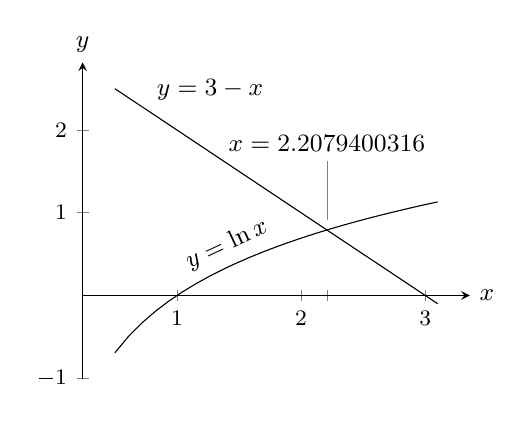
\begin{tikzpicture}[font=\small]
\begin{axis}[small,axis lines=middle,xlabel={$x$},ylabel={$y$},xlabel style={at={(current axis.right of origin)},anchor=west},ylabel style={at={(current axis.above origin)},anchor=south},enlargelimits=true,xtick={1,2,2.2079,3},xticklabels={1,2,,3}]
\addplot[domain=0.5:3.1]{ln(x)}node[pos=0.45,sloped,above]{$y=\ln x$};
\addplot[domain=0.5:3.1]{3-x}node[pos=0.1,above right]{$y=3-x$};
\draw(axis cs:2.2079,0.7921)node[pin={[pin distance=0.75cm]90:{$x=\num{2.2079400316}$}}]{};
\end{axis}
\end{tikzpicture}
\caption{نقطہ قطع}
\end{subfigure}\hfill
\begin{subfigure}{0.45\textwidth}
\centering
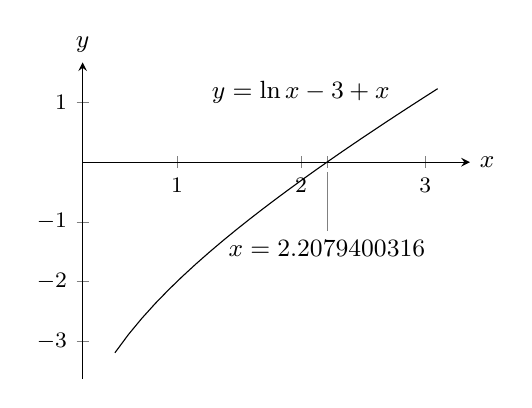
\begin{tikzpicture}[font=\small]
\begin{axis}[small,axis lines=middle,xlabel={$x$},ylabel={$y$},xlabel style={at={(current axis.right of origin)},anchor=west},ylabel style={at={(current axis.above origin)},anchor=south},enlargelimits=true,xtick={1,2,2.2079,3},xticklabels={1,2,,3}]
\addplot[domain=0.5:3.1]{ln(x)-3+x}node[pos=0.9,above left]{$y=\ln x-3+x$};
\draw(axis cs:2.2079,0)node[pin={[pin distance=0.75cm]-90:{$x=\num{2.2079400316}$}}]{};
\end{axis}
\end{tikzpicture}
\caption{جذر}
\end{subfigure}
\caption{تفاعل $f(x)$ اور $g(x)$ کے حل کی تلاش۔}
\label{شکل_تکمل_استعمال_نقطہ_قطع}
\end{figure}

\جزوحصہ{تبدیل ہوتے کلیات والا سرحد}
اگر سرحد کا کلیہ ایک یا ایک سے زیادہ نقطوں پر تبدیل ہوتا ہو تب ہم خطہ کو مطابقتی ذیلی خطوں میں تقسیم کرتے ہوئے ہر ذیلی خطے پر علیحدہ علیحدہ مساوات \حوالہ{مساوات_تکمل_استعمال_رقبہ_تعریف} کا اطلاق کرتے ہیں۔

\ابتدا{مثال}\شناخت{مثال_استعمال_تکمل_تبدیل_کلیہ}
ربع اول میں \عددی{y=\sqrt{x}} کے نیچے  اور \عددی{y=x-2} کے اوپر رقبہ تلاش کریں۔

حل:\quad
\موٹا{پہلا قدم:}\quad
ترسیم (شکل \حوالہ{شکل_مثال_استعمال_تکمل_تبدیل_کلیہ}) سے ہم دیکھتے ہیں کہ خطے کی بالائی سرحد \عددی{f(x)=\sqrt{x}} ہے جبکہ \عددی{0\le x\le 2}  پر اس کی نچلی سرحد \عددی{g(x)=0} اور \عددی{2\le x\le 4} پر نچلی سرحد \عددی{g(x)=x-2} ہے (نقطہ \عددی{x=2} پر \عددی{g(x)} کے دونوں کلیات ایک جیسے ہیں)۔ ہم \عددی{x=2} پر خطہ کو دو ذیلی حصوں \عددی{A} اور \عددی{B} میں تقسیم کر کے دونوں ذیلی خطوں کے لئے نمائندہ مستطیل بناتے ہیں۔\\
\موٹا{دوسرا قدم:}\quad
خطہ \عددی{A} میں تکمل کے حد \عددی{a=0} اور \عددی{b=2} ہیں۔ خطہ \عددی{B} کا بایاں حد \عددی{a=2} ہے۔اس کے دایاں حد جاننے کے لئے ہم مساوات  \عددی{y=\sqrt{x}} اور  \عددی{y=x-2} کو ایک ساتھ حل کرتے ہیں۔
\begin{align*}
\sqrt{x}&=x-2&&\text{\RL{$f(x)$ اور $g(x)$ کے برابر پر کریں}}\\
x&=(x-2)^2=x^2-4x+4&&\text{\RL{مربع لیں}}\\
x^2-5x+4&=0&&\text{\RL{ایک جانب منتقلی}}\\
(x-1)(x-4)&=0&&\text{\RL{تجزی}}\\
x=1,\quad x&=4&&\text{\RL{حل}}
\end{align*}
صرف \عددی{x=4} مساوات \عددی{\sqrt{x}=x-2} کو مطمئن کرتا ہے جبکہ مربع لینے کی وجہ سے حل \عددی{x=1} پیدا ہوا ہے جس کو رد کیا جاتا ہے۔ یوں دایاں حد \عددی{b=4} ہے۔\\
\موٹا{تیسرا قدم:}
\begin{align*}
f(x)-g(x)&=\sqrt{x}-0=\sqrt{x},&& 0\le x\le 2\\
f(x)-g(x)&=\sqrt{x}-(x-2)=\sqrt{x}-x+2,&&2\le x\le 4
\end{align*}
\موٹا{چوتھا قدم:}\quad
ہم خطہ \عددی{A} اور \عددی{B} کے رقبوں کا مجموعہ لیتے ہیں۔
\begin{align*}
S&=\int_0^2\sqrt{x}\dif x+\int_2^4(\sqrt{x}-x+2)\dif x\\
&=\big[\frac{2}{3}x^{3/2}\big]_0^2+\big[\frac{2}{3}x^{3/2}-\frac{x^2}{2}+2x\big]_2^4\\
&=\frac{2}{3}(2)^{3/2}-0+\big(\frac{2}{3}(4)^{3/2}-8+8\big)-\big(\frac{2}{3}(2)^{3/2}-2+4\big)\\
&=\frac{2}{3}(8)-2=\frac{10}{3}
\end{align*}
\انتہا{مثال}
%=========================
\begin{figure}
\centering
\begin{tikzpicture}[declare function={f(\x)=sqrt(\x);g(\x)=\x-2;}]
\begin{axis}[clip=false,axis on top,small,axis lines=middle,xlabel={$x$},ylabel={$y$},xtick={2,4},ytick={2,4},enlargelimits=true,xlabel style={at={(current axis.right of origin)},anchor=west},ylabel style={at={(current axis.above origin)},anchor=south}]
\addplot[name path=kfa,domain=0:0.5,draw=none]{f(x)};
\addplot[name path=kfb,domain=0.5:2,draw=none]{f(x)};
\draw[name path=axisfa](axis cs:0,0)--(axis cs:0.5,0);
\draw[name path=axisfb](axis cs:0.5,0)--(axis cs:2,0);
\addplot[fill=lgray] fill between [of =kfa and axisfa];
\addplot[fill=lgray] fill between [of =kfb and axisfb];
\addplot[domain=0:0.5]{f(x)};
\addplot[domain=0.5:4.2]{f(x)};
\addplot[domain=1.8:4.2]{g(x)}node[pos=0.75,right]{$y=x-2$};
\draw(axis cs:2.25,{f(2.25)})node[pin=135:{$y=\sqrt{x}$}]{};
\pgfmathsetmacro{\k}{1}
\pgfmathsetmacro{\w}{0.5}
\draw(axis cs:\k,{f(\k+\w/2)})--(\k+\w,{f(\k+\w/2)})coordinate(kTR)--(\k+\w,0)coordinate(kBR)--(\k,0)coordinate(kBL)--(\k,{f(\k+\w/2)})coordinate(kTL);
\draw[stealth-stealth]($(kBL)!0.75!(kTL)$)--($(kBR)!0.75!(kTR)$)node[pos=0.5,below]{$\Delta x$};
\draw(axis cs:\k+\w/2,{f(\k+\w/2)})node[circ]{}node[above]{$(x,f(x))$};
\draw(axis cs:\k+\w/2,0)node[circ]{}node[below,xshift=-0.75ex,yshift=-1ex]{$(x,g(x))$};
\draw(axis cs:2,{f(2)})--(axis cs:2,0);
\pgfmathsetmacro{\kk}{2.5}
\pgfmathsetmacro{\ww}{0.5}
\draw(axis cs:\kk,{f(\kk+\ww/2)})--(\kk+\ww,{f(\kk+\ww/2)})coordinate(kTR)--
(\kk+\ww, {g(\kk+\ww/2)})coordinate(kBR)--(\kk,{g(\kk+\ww/2)})coordinate(kBL)--(\kk,{f(\kk+\ww/2)})coordinate(kTL);
\draw[stealth-stealth]($(kBL)!0.75!(kTL)$)--($(kBR)!0.75!(kTR)$)node[pos=0.5,below]{$\Delta x$};
\draw(axis cs:\kk+\ww/2,{f(\kk+\ww/2)})node[circ]{}node[above,xshift=-0.5ex,yshift={0.5ex}]{$(x,f(x))$};
\draw(axis cs:\kk+\ww/2,{g(\kk+\ww/2)})node[circ]{}node[below right]{$(x,g(x))$};
\draw(axis cs:0.5,0.35)node[]{$A$};
\draw(axis cs:3.35,1.6)node[]{$B$};
\end{axis}
\end{tikzpicture}
\caption{خطہ برائے مثال \حوالہ{مثال_استعمال_تکمل_تبدیل_کلیہ}}
\label{شکل_مثال_استعمال_تکمل_تبدیل_کلیہ}
\end{figure}
\جزوحصہء{تکمل بلحاظ $y$}
اگر سرحد کی مساواتیں \عددی{y} کی تفاعل ہوں تب تخمینی مستطیل کو انتصابی کی بجائے افقی بنایا جاتا ہے اور بنیادی کلیہ میں \عددی{x} کی جگہ \عددی{y} پایا جائے گا (شکل \حوالہ{شکل_استعمال_تکمل_وائے_سرحد}):
\begin{align}\label{مساوات_تکمل_استعمال_رقبہ_تعریف_دوم}
S=\int_c^d[f(y)-g(y)]\dif y
\end{align}
%
\begin{figure}
\centering
\begin{minipage}{0.3\textwidth}
\centering
\begin{tikzpicture}[font=\small,declare function={g(\x)=-1+\x^3-\x;f(\x)=1+0.5*\x^3-\x;}]
\begin{axis}[clip=false,width=5cm,axis lines=middle,xlabel={$x$},ylabel={$y$},xlabel style={at={(current axis.right of origin)},anchor=west},ylabel style={at={(current axis.above origin)},anchor=south},xtick={\empty},ytick={\empty},enlargelimits=true]
\addplot[domain=-1.2:1.2]({f(x)},{\x})node[pos=0.82,right]{$x=f(y)$};
\addplot[domain=-1.2:1.1]({g(x)},{\x})node[pos=0.35,left]{$x=g(y)$};
\draw(axis cs:{f(1)},1)--(axis cs:{g(1)},1)node[pos=0.6,above]{$d$};
\draw(axis cs:{f(-1)},-1)--(axis cs:{g(-1)},-1)node[pos=0.25,below]{$c$};
\draw(axis cs:{f(0.5)},0.5)--(axis cs:{g(0.5)},0.5);
\draw(axis cs:{f(0.4)},0.4)--(axis cs:{g(0.4)},0.4);
\addplot[name path=funf,domain=0.4:0.5,draw=none]({f(x)},{\x});
\addplot[name path=fung,domain=0.4:0.5,draw=none]({g(x)},{\x});
\addplot[fill=lgray]fill between [of = funf and fung];
\end{axis}
\end{tikzpicture}
\end{minipage}\hfill
\begin{minipage}{0.3\textwidth}
\centering
\begin{tikzpicture}[font=\small,declare function={g(\x)=1+\x^2-3*\x+2;f(\x)=1-\x^2+4*\x-3;}]
\begin{axis}[width=5cm,axis lines=middle,xlabel={$x$},ylabel={$y$},xlabel style={at={(current axis.right of origin)},anchor=west},ylabel style={at={(current axis.above origin)},anchor=south},xtick={\empty},ytick={1,1.8},yticklabels={$c$,$d$},xmin=0,ymin=0,enlargelimits=true]
\addplot[domain=0.9:2]({f(x)},{\x})node[pos=0.3,right,yshift=-0.5ex]{$x=f(y)$};
\addplot[domain=0.9:2]({g(x)},{\x})node[pos=0.35,left]{$x=g(y)$};
\draw(axis cs:{f(1.8)},1.8)--(axis cs:{g(1.8)},1.8);
\draw(axis cs:{f(1.5)},1.5)--(axis cs:{g(1.5)},1.5);
\draw(axis cs:{f(1.6)},1.6)--(axis cs:{g(1.6)},1.6);
\addplot[name path=funf,domain=1.5:1.6,draw=none]({f(x)},{\x});
\addplot[name path=fung,domain=1.5:1.6,draw=none]({g(x)},{\x});
\addplot[fill=lgray]fill between [of = funf and fung];
\end{axis}
\end{tikzpicture}
\end{minipage}\hfill
\begin{minipage}{0.3\textwidth}
\centering
\begin{tikzpicture}[font=\small,declare function={g(\x)=1+\x^2-3*\x+2;f(\x)=1-\x^2+4*\x-3;}]
\begin{axis}[clip=false,width=5cm,axis lines=middle,xlabel={$x$},ylabel={$y$},xlabel style={at={(current axis.right of origin)},anchor=west},ylabel style={at={(current axis.above origin)},anchor=south},xtick={\empty},ytick={1,2.5},yticklabels={$c$,$d$},xmin=0,ymin=0,enlargelimits=true]
\addplot[domain=0.9:2.6]({f(x)},{\x})node[pos=0.3,below right]{$x=f(y)$};
\addplot[domain=0.9:2.6]({g(x)},{\x})node[pos=0.65,above left]{$x=g(y)$};
\draw(axis cs:{f(1.5)},1.5)--(axis cs:{g(1.5)},1.5);
\draw(axis cs:{f(1.6)},1.6)--(axis cs:{g(1.6)},1.6);
\addplot[name path=funf,domain=1.5:1.6,draw=none]({f(x)},{\x});
\addplot[name path=fung,domain=1.5:1.6,draw=none]({g(x)},{\x});
\addplot[fill=lgray]fill between [of = funf and fung];
\end{axis}
\end{tikzpicture}
\end{minipage}
\caption{ان اشکال میں دایاں سرحد $f$ اور بایاں سرحد $g$ ہو گا لہٰذا $f(y)-g(y)$ غیر منفی ہو گا۔}
\label{شکل_استعمال_تکمل_وائے_سرحد}
\end{figure}

\ابتدا{مثال}\شناخت{مثال_استعمال_تکمل_تبدیل_کلیہ_دوم}
درج بالا مثال \حوالہ{مثال_استعمال_تکمل_تبدیل_کلیہ} کو اس بار مساوات \حوالہ{مساوات_تکمل_استعمال_رقبہ_تعریف_دوم} کی مدد سے حل کریں۔

حل:\quad
\موٹا{پہلا قدم:}\quad
ہم خطہ ترسیم کر کے نمائندہ افقی مستطیل بناتے ہیں (شکل \حوالہ{شکل_استعمال_تکمل_وائے_سرحد})۔ خطے کا دایاں سرحد لکیر \عددی{x=y+2} ہے لہٰذا \عددی{f(y)=y+2} ہو گا۔خطے کا بایاں سرحد \عددی{x=y^2} ہے لہٰذا \عددی{g(y)=y^2} ہو گا۔\\
\موٹا{دوسرا قدم:}\quad
تکمل کا زیریں حد \عددی{y=0} ہے۔ تکمل کا بالائی حد جاننے کے لئے ہم \عددی{x=y+2} اور \عددی{x=y^2} کو \عددی{y} کے لئے حل کرتے ہیں:
\begin{align*}
y+2&=y^2&&\text{\RL{$f$ کو $g$ کے برابر پر کرتے ہیں}}\\
y^2-y-2&=0\text{\RL{ایک ہاتھ منتقلی}}\\
(y+1)(y-2)&=0\text{\RL{تجزی}}\\
y=-1,\quad y&=2\text{\RL{حل}}
\end{align*}
تکمل کا بالائی حد \عددی{y=2} ہے (چونکہ \عددی{y=-1} افقی محور سے نیچے تفاعل کا نقطہ قطع دیتا ہے)۔\\
\موٹا{تیسرا قدم:}\quad
\begin{align*}
f(y)-g(y)=y+2-y^2=2+y-y^2
\end{align*}
\موٹا{چوتھا قدم:}\quad
\begin{align*}
S=\int_a^b[f(y)-g(y)]\dif y&=\int_0^2[2+y-y^2]\dif y\\
&=\big[2y+\frac{y^2}{2}-\frac{y^3}{3}\big]_0^2\\
&=4+\frac{4}{2}-\frac{8}{3}=\frac{10}{3}
\end{align*}
یہ وہی جواب ہے جو مثال \حوالہ{مثال_استعمال_تکمل_تبدیل_کلیہ} میں حاصل کی گیا۔ مثال \حوالہ{مثال_استعمال_تکمل_تبدیل_کلیہ} میں دو تکمل حل کرنے کی ضرورت پیش آئی جبکہ یہاں ایک ہی تکمل سے رقبہ معلوم کرنا ممکن تھا۔
\انتہا{مثال}
%======================
\begin{figure}
\centering
\begin{minipage}{0.45\textwidth}
\centering
\begin{tikzpicture}[declare function={f(\x)=\x+2;g(\x)=\x^2;}]
\begin{axis}[clip=false,axis on top,small,axis lines=middle,xlabel={$x$},ylabel={$y$},xtick={2,4},ytick={2,4},enlargelimits=true,xlabel style={at={(current axis.right of origin)},anchor=west},ylabel style={at={(current axis.above origin)},anchor=south}]
\addplot[domain=0:2]({f(x)},x)node[pos=0.75,right]{$x=y+2$};
\addplot[domain=0:2]({g(x)},x)node[pos=0.75,above]{$x=y^2$};
\pgfmathsetmacro{\k}{0.9}
\pgfmathsetmacro{\w}{0.5}
\draw(axis cs:{g(\k)},\k+\w/2)--(axis cs:{f(\k)},\k+\w/2)coordinate(kTR)--(axis cs:{f(\k)},\k-\w/2)coordinate(kBR)--(axis cs:{g(\k)},\k-\w/2)coordinate(kBL)--(axis cs:{g(\k)},\k+\w/2)coordinate(kTL);
\draw[stealth-stealth]($(kBL)!0.75!(kBR)$)--($(kTL)!0.75!(kTR)$)node[pos=0.5,left]{$\Delta y$};
\draw(axis cs:1,0)node[below]{$y=0$};
\draw[stealth-stealth] (axis cs:{g(\k)},\k-0.75*\w)--(axis cs:{f(\k)},\k-0.75*\w)node[pos=0.5,below]{$f(y)-g(y)$};
\draw(axis cs:{f(\k)},\k)node[circ]{}node[right]{$(f(y),y)$};
\draw(axis cs:{g(\k)},\k)node[circ]{}node[left]{$(g(y),y)$};
\draw(axis cs:4,2)node[right]{$(4,2)$};
\draw(axis cs:0,0)node[below left,font=\footnotesize]{$0$};
\end{axis}
\end{tikzpicture}
\caption{خطہ برائے مثال \حوالہ{مثال_استعمال_تکمل_تبدیل_کلیہ_دوم}}
\label{شکل_مثال_استعمال_تکمل_تبدیل_کلیہ_دوم}
\end{minipage}\hfill
\begin{minipage}{0.45\textwidth}
\centering
\begin{tikzpicture}[declare function={f(\x)=sqrt(\x);g(\x)=\x-2;}]
\begin{axis}[clip=false,axis on top,small,axis lines=middle,xlabel={$x$},ylabel={$y$},xtick={2,4},ytick={2,4},enlargelimits=true,xlabel style={at={(current axis.right of origin)},anchor=west},ylabel style={at={(current axis.above origin)},anchor=south}]
\addplot[domain=0.5:4]{f(x)}node[pos=0.5,above left]{$y=\sqrt{x}$};
\addplot[domain=0:0.5]{f(x)};
\addplot[name path=fung,domain=2:4]{g(x)}node[pos=0.3,above left]{$y=x-2$};
\draw(axis cs:1,0)node[below]{$y=0$};
\draw(axis cs:4,2)node[right]{$(4,2)$};
\draw(axis cs:0,0)node[below left,font=\footnotesize]{$0$};
\addplot[name path=funf,domain=2:4,draw=none]{g(x)};
\path[name path=kaxis](axis cs:2,0)--(axis cs:4,0);
\addplot[fill=llgray]fill between[of=kaxis and funf];
\draw(axis cs:3,0)node[above]{$2$}  (axis cs:4,1)node[left]{$2$};
\end{axis}
\end{tikzpicture}
\caption{بالائی منحنی کے نیچے خطہ سے تکون منفی کرنے سے رقبہ حاصل ہو گا۔}
\label{شکل_مثال_استعمال_تکمل_تبدیل_کلیہ_سوم}
\end{minipage}\hfill
\end{figure}

\جزوحصہء{تکمل کے ساتھ جیومیٹریائی کلیات کا استعمال}
تکمل اور جیومیٹریائی کلیات کو ملا کر رقبہ نسبتاً زیادہ جلد حاصل ہوتا ہے۔

\ابتدا{مثال}\شناخت{مثال_استعمال_تکمل_تبدیل_کلیہ_سوم}
مزید ایک بار مثال \حوالہ{مثال_استعمال_تکمل_تبدیل_کلیہ} میں دیے گئے خطے کا رقبہ تلاش کریں۔

حل:\quad
ہم \عددی{0\le x\le 4} محور \عددی{x}  اور \عددی{y=\sqrt{x}} کے بیچ رقبہ سے قاعدہ \عددی{2} اور قد \عددی{2} کے تکون کا رقبہ منفی کرتے ہوئے درکار خطے کا رقبہ تلاش کر سکتے ہیں۔ 
\begin{align*}
S&=\int_0^4\sqrt{x}\dif x-\frac{1}{2}(2)(2)\\
&=\left. \frac{2}{3}x^{3/2}\right]_0^4-2\\
&=\frac{2}{3}(8)-0-2=\frac{10}{3}
\end{align*}
\انتہا{مثال}
%===================================

گزشتہ تین مثالوں میں آپ نے دیکھا کہ دو منحنیات کے بیچ رقبہ بعض اوقات \عددی{x} کی بجائے \عددی{y} کے ساتھ تکمل لے کر نسبتاً آسانی سے حاصل ہوتا ہے۔ اسی طرح بعض اوقات تکمل اور جیومیٹری کے کلیات کو ملا کر جلد جواب حاصل ہوتا ہے۔ یوں تکمل لکھنے سے پہلے مسئلے پر غور کرنا بہتر ہو گا۔

\حصہء{سوالات}

سوال \حوالہ{سوال_استعمال_تکمل_سایہ_دار_الف} تا سوال \حوالہ{سوال_استعمال_تکمل_سایہ_دار_ب} میں سایہ دار رقبہ تلاش کریں۔

\ابتدا{سوال}\شناخت{سوال_استعمال_تکمل_سایہ_دار_الف}
سایہ دار خطہ شکل \حوالہ{شکل_سوال_استعمال_تکمل_سایہ_دار_الف} جہاں سرحد \عددی{y=1} اور \عددی{y=\cos^2x} ہیں۔\\
جواب:\quad
$\tfrac{\pi}{2}$
\انتہا{سوال}
%========================
\ابتدا{سوال}\شناخت{سوال_استعمال_تکمل_سایہ_دار_پ}
سایہ دار خطہ شکل \حوالہ{شکل_سوال_استعمال_تکمل_سایہ_دار_پ} جہاں سرحد \عددی{y=\tfrac{1}{2}\sec^2t}، \عددی{y=-4\sin^2t}، \عددی{y=-\tfrac{\pi}{3}} اور \عددی{y=\tfrac{\pi}{3}} ہیں۔
\انتہا{سوال}
%========================
\ابتدا{سوال}\شناخت{سوال_استعمال_تکمل_سایہ_دار_ت}
سایہ دار خطہ شکل \حوالہ{شکل_سوال_استعمال_تکمل_سایہ_دار_ت} جہاں سرحد \عددی{x=y^3} اور \عددی{x=y^2} ہیں۔\\
جواب:\quad
$\tfrac{1}{12}$
\انتہا{سوال}
%========================
\ابتدا{سوال}\شناخت{سوال_استعمال_تکمل_سایہ_دار_ٹ}
سایہ دار خطہ شکل \حوالہ{شکل_سوال_استعمال_تکمل_سایہ_دار_ٹ} جہاں سرحد \عددی{x=12y^2-12y^3} اور \عددی{x=2y^2-2y} ہیں۔
\انتہا{سوال}
%========================
\ابتدا{سوال}\شناخت{سوال_استعمال_تکمل_سایہ_دار_ث}
سایہ دار خطہ شکل \حوالہ{شکل_سوال_استعمال_تکمل_سایہ_دار_ث} جہاں سرحد \عددی{y=2x^2} اور \عددی{y=x^4-2x^2} ہیں۔\\
جواب:\quad
$\tfrac{128}{15}$
\انتہا{سوال}
%========================
\ابتدا{سوال}\شناخت{سوال_استعمال_تکمل_سایہ_دار_ج}
سایہ دار خطہ شکل \حوالہ{شکل_سوال_استعمال_تکمل_سایہ_دار_ج} جہاں سرحد \عددی{y=x^2}، \عددی{y=-2x^4}، \عددی{x=-1} اور \عددی{x=1} ہیں۔
\انتہا{سوال}
%========================
\ابتدا{سوال}\شناخت{سوال_استعمال_تکمل_سایہ_دار_چ}
سایہ دار خطہ شکل \حوالہ{شکل_سوال_استعمال_تکمل_سایہ_دار_چ} جہاں سرحد \عددی{y=1}، \عددی{y=x} اور \عددی{y=\tfrac{x^2}{4}} ہیں۔\\
جواب:\quad
$\tfrac{5}{6}$
\انتہا{سوال}
%========================
\ابتدا{سوال}\شناخت{سوال_استعمال_تکمل_سایہ_دار_ب}
سایہ دار خطہ شکل \حوالہ{شکل_سوال_استعمال_تکمل_سایہ_دار_ب} جہاں سرحد \عددی{y=x^2}، \عددی{y=2-x} اور \عددی{y=0} ہیں۔
\انتہا{سوال}
%========================
\begin{figure}
\centering
\begin{minipage}{0.22\textwidth}
\centering
\begin{tikzpicture}[font=\tiny,declare function={f(\x)=(cos(deg(\x)))^2;g(\x)=1;}]
\begin{axis}[axis on top,clip=false,width=4cm,axis lines=middle,xlabel={$x$},ylabel={$y$},xtick={1.571,3.142},xticklabels={$\tfrac{\pi}{2}$,$\pi$},ytick={1},enlargelimits=true,xlabel style={at={(current axis.right of origin)},anchor=west},ylabel style={at={(current axis.above origin)},anchor=south}]
\addplot[domain=-0.25:3.2,smooth]{f(x)}node[pos=0.75,right]{$y=\cos^2x$};
\addplot[domain=-0.25:3.2]{g(x)}node[pos=0.5,above]{$y=1$};
\addplot[name path=funf,domain=0:3.142,draw=none]{f(x)};
\addplot[name path=fung,domain=0:3.142,draw=none]{g(x)};
\addplot[fill=lgray]fill between[of=funf and fung];
\end{axis}
\end{tikzpicture}
\caption{}
\label{شکل_سوال_استعمال_تکمل_سایہ_دار_الف}
\end{minipage}\hfill
\begin{minipage}{0.22\textwidth}
\centering
\begin{tikzpicture}[font=\tiny,declare function={f(\x)=1/2*(sec(deg(\x)))^2;g(\x)=-4*(sin(deg(\x)))^2;}]
\pgfmathsetmacro{\k}{pi/3}
\begin{axis}[axis on top,clip=false,width=4cm,axis lines=middle,xlabel={$t$},ylabel={$y$},xtick={-1.047,1.047},xticklabels={$-\tfrac{\pi}{3}$,$\tfrac{\pi}{3}$},ytick={-2,1,2},enlargelimits=true,xlabel style={at={(current axis.right of origin)},anchor=west},ylabel style={at={(current axis.above origin)},anchor=south}]
\addplot[name path=funf,domain=-\k:\k,smooth]{f(x)}node[pos=0.75,sloped,above,xshift=0.5ex]{$y=\tfrac{1}{2}\sec^2t$};
\addplot[name path=fung,domain=-\k:\k]{g(x)}node[pos=0.75,sloped,below]{$y=-4\sin^2t$};
\addplot[fill=lgray]fill between[of=funf and fung];
\end{axis}
\end{tikzpicture}
\caption{}
\label{شکل_سوال_استعمال_تکمل_سایہ_دار_پ}
\end{minipage}\hfill
\begin{minipage}{0.22\textwidth}
\centering
\begin{tikzpicture}[font=\tiny,declare function={f(\x)=(\x)^(1/3);g(\x)=(\x)^(1/2);}]
\begin{axis}[axis on top,clip=false,width=4cm,axis lines=middle,xlabel={$x$},ylabel={$y$},xtick={1},ytick={1},enlargelimits=true,xlabel style={at={(current axis.right of origin)},anchor=west},ylabel style={at={(current axis.above origin)},anchor=south}]
\addplot[domain=0:0.5]{f(x)};
\addplot[domain=0.5:1.25]{f(x)}node[pos=0.25,above]{$x=y^3$};
\addplot[domain=0:0.5]{g(x)};
\addplot[domain=0.5:1.25]{g(x)}node[pos=0.25,below]{$x=y^2$};
\addplot[name path=funf,domain=0:1,draw=none]{f(x)};
\addplot[name path=fung,domain=0:1,draw=none]{g(x)};
\addplot[fill=lgray]fill between[of=funf and fung];
\draw(axis cs:1,1)node[circ]{}node[below]{$(1,1)$};
\end{axis}
\end{tikzpicture}
\caption{}
\label{شکل_سوال_استعمال_تکمل_سایہ_دار_ت}
\end{minipage}\hfill
\begin{minipage}{0.22\textwidth}
\centering
\begin{tikzpicture}[font=\tiny,declare function={f(\x)=12*\x^2-12*\x^3;g(\x)=2*\x^2-2*\x;}]
\pgfmathsetmacro{\k}{pi/3}
\begin{axis}[axis on top,clip=false,width=4cm,axis lines=middle,xlabel={$t$},ylabel={$y$},xtick={1} ,ytick={1},enlargelimits=true,xlabel style={at={(current axis.right of origin)},anchor=west},ylabel style={at={(current axis.above origin)},anchor=south}]
\addplot[domain=-0.2:1.02]({f(x)},{x})node[pos=0.65,above]{$x=12y^2-12y^3$};
\addplot[domain=-0.1:1.2]({g(x)},{x})node[pos=0.45,sloped,above]{$x=2y^2-2y$};
\addplot[name path=funf,domain=0:1,draw=none]({f(x)},{x});
\addplot[name path=fung,domain=0:1,draw=none]({g(x)},{x});
\addplot[fill=lgray]fill between[of=funf and fung];
\end{axis}
\end{tikzpicture}
\caption{}
\label{شکل_سوال_استعمال_تکمل_سایہ_دار_ٹ}
\end{minipage}
\end{figure}
%
\begin{figure}
\centering
\begin{minipage}{0.22\textwidth}
\centering
\begin{tikzpicture}[font=\tiny,declare function={f(\x)=2*\x^2;g(\x)=\x^4-2*\x^2;}]
\begin{axis}[axis on top,clip=false,width=4cm,axis lines=middle,xlabel={$x$},ylabel={$y$},xtick={-2,2}, xticklabels={$2$,$2$},ytick={-1,8},enlargelimits=true,xlabel style={at={(current axis.right of origin)},anchor=west},ylabel style={at={(current axis.above origin)},anchor=south}]
\addplot[name path=funf,domain=-2:2]{f(x)}node[pos=0.85,left]{$y=2x^2$};
\addplot[name path=fung,domain=-2:2]{g(x)}node[pos=0.85,sloped,below]{$y=x^4-2x^2$};
%\addplot[name path=funf,domain=0:3.142,draw=none]{f(x)};
%\addplot[name path=fung,domain=0:3.142,draw=none]{g(x)};
\addplot[fill=lgray]fill between[of=funf and fung];
\draw(axis cs:-2,8)node[circ]{}node[above]{$(-2,8)$}  (axis cs:2,8)node[circ]{}node[above]{$(2,8)$};
\end{axis}
\end{tikzpicture}
\caption{}
\label{شکل_سوال_استعمال_تکمل_سایہ_دار_ث}
\end{minipage}\hfill
\begin{minipage}{0.22\textwidth}
\centering
\begin{tikzpicture}[font=\tiny,declare function={f(\x)=\x^2;g(\x)=-2*\x^4;}]
\begin{axis}[axis on top,clip=false,width=4cm,axis lines=middle,xlabel={$x$},ylabel={$y$},xtick={-1,1}, xticklabels={$-1$,$1$},ytick={-2,1},enlargelimits=true,xlabel style={at={(current axis.right of origin)},anchor=west},ylabel style={at={(current axis.above origin)},anchor=south}]
\addplot[name path=funf,domain=-1:1]{f(x)}node[pos=0.85,left]{$y=x^2$};
\addplot[name path=fung,domain=-1:1]{g(x)}node[pos=0.85,left]{$y=-2x^4$};
%\addplot[name path=funf,domain=0:3.142,draw=none]{f(x)};
%\addplot[name path=fung,domain=0:3.142,draw=none]{g(x)};
\addplot[fill=lgray]fill between[of=funf and fung];
\end{axis}
\end{tikzpicture}
\caption{}
\label{شکل_سوال_استعمال_تکمل_سایہ_دار_ج}
\end{minipage}\hfill
\begin{minipage}{0.22\textwidth}
\centering
\begin{tikzpicture}[font=\tiny,declare function={f(\x)=\x;g(\x)=1/4*\x^2;}]
\begin{axis}[axis on top,clip=false,width=4cm,axis lines=middle,xlabel={$x$},ylabel={$y$},xtick={1,2}, xticklabels={$1$,$2$},ytick={1},enlargelimits=true,xlabel style={at={(current axis.right of origin)},anchor=west},ylabel style={at={(current axis.above origin)},anchor=south}]
\addplot[domain=0:1.5]{f(x)}node[pos=0.9,left]{$y=x$};
\addplot[domain=0:2.2]{g(x)}node[pos=0.7,below right]{$y=\frac{1}{4}x^2$};
\addplot[name path=funf,domain=0:1,draw=none]{f(x)};
\addplot[name path=fung,domain=0:2,draw=none]{g(x)};
\addplot[fill=lgray]fill between[of=funf and fung];
\draw(axis cs:0.75,1)--(axis cs:2.25,1)node[pos=0.55,above]{$y=1$};
\end{axis}
\end{tikzpicture}
\caption{}
\label{شکل_سوال_استعمال_تکمل_سایہ_دار_چ}
\end{minipage}\hfill
\begin{minipage}{0.22\textwidth}
\centering
\begin{tikzpicture}[font=\tiny,declare function={f(\x)=2-\x;g(\x)=\x^2;}]
\begin{axis}[axis on top,clip=false,width=4cm,axis lines=middle,xlabel={$x$},ylabel={$y$},xtick={1,2}, xticklabels={$1$,$2$},ytick={1},enlargelimits=true,xlabel style={at={(current axis.right of origin)},anchor=west},ylabel style={at={(current axis.above origin)},anchor=south}]
\addplot[domain=0.75:2]{f(x)}node[pos=0.5,right]{$y=2-x$};
\addplot[domain=0:1.1]{g(x)}node[pos=0.6,left]{$y=x^2$};
\addplot[name path=funf,domain=1:2,draw=none]{f(x)};
\addplot[name path=fung,domain=0:1,draw=none]{g(x)};
\draw[name path=axisf](axis cs:1,0)--(axis cs:2,0);
\draw[name path=axisg](axis cs:0,0)--(axis cs:1,0);
\addplot[fill=lgray]fill between[of=funf and axisf];
\addplot[fill=lgray]fill between[of=fung and axisg];
\end{axis}
\end{tikzpicture}
\caption{}
\label{شکل_سوال_استعمال_تکمل_سایہ_دار_ب}
\end{minipage}
\end{figure}

سوال \حوالہ{سوال_استعمال_تکمل_کل_سایہ_دار_رقبہ_الف} تا سوال \حوالہ{سوال_استعمال_تکمل_کل_سایہ_دار_رقبہ_ب} میں کل سایہ دار رقبہ تلاش کریں۔

\ابتدا{سوال}\شناخت{سوال_استعمال_تکمل_کل_سایہ_دار_رقبہ_الف}
سایہ دار رقبہ شکل \حوالہ{شکل_سوال_استعمال_تکمل_کل_سایہ_دار_رقبہ_الف} جہاں سرحد \عددی{y=x^2-4}، \عددی{y=-x^2-2x} اور \عددی{x=-3} ہیں۔\\
جواب:\quad
$\tfrac{38}{3}$
\انتہا{سوال}
%=======================
\ابتدا{سوال}\شناخت{سوال_استعمال_تکمل_کل_سایہ_دار_رقبہ_پ}
سایہ دار رقبہ شکل \حوالہ{شکل_سوال_استعمال_تکمل_کل_سایہ_دار_رقبہ_پ} جہاں سرحد \عددی{y=-x^2+3x} اور \عددی{y=2x^3-x^2-5x} ہیں۔
\انتہا{سوال}
%=======================
\ابتدا{سوال}\شناخت{سوال_استعمال_تکمل_کل_سایہ_دار_رقبہ_ت}
سایہ دار رقبہ شکل \حوالہ{شکل_سوال_استعمال_تکمل_کل_سایہ_دار_رقبہ_ت} جہاں سرحد \عددی{y=4-x^2}، \عددی{y=2-x}، \عددی{x=-2} اور \عددی{x=3} ہیں۔\\
جواب:\quad
$\tfrac{49}{6}$
\انتہا{سوال}
%=======================
\ابتدا{سوال}\شناخت{سوال_استعمال_تکمل_کل_سایہ_دار_رقبہ_ب}
سایہ دار رقبہ شکل \حوالہ{شکل_سوال_استعمال_تکمل_کل_سایہ_دار_رقبہ_ب} جہاں سرحد \عددی{y=\tfrac{x^3}{3}-x}، \عددی{y=\tfrac{x}{3}} اور \عددی{x=3} ہیں۔
\انتہا{سوال}
%=======================
\begin{figure}
\centering
\begin{minipage}{0.22\textwidth}
\centering
\begin{tikzpicture}[font=\tiny,declare function={f(\x)=\x^2-4;g(\x)=-\x^2-2*\x;}]
\begin{axis}[axis on top,clip=false,width=4cm,axis lines=middle,xlabel={$x$},ylabel={$y$},xtick={-3,1},ytick={-4,5}, enlargelimits=true,xlabel style={at={(current axis.right of origin)},anchor=west},ylabel style={at={(current axis.above origin)},anchor=south}]
\addplot[domain=-3:1.1,smooth]{f(x)}node[pos=0.15,right]{$y=x^2-4$};
\addplot[domain=-3:1.1]{g(x)}node[pos=0.5,pin=30:{$y=-x^2-2x$}]{};
\addplot[name path=funf,domain=-3:1,draw=none]{f(x)};
\addplot[name path=fung,domain=-3:1,draw=none]{g(x)};
\addplot[fill=lgray]fill between[of=funf and fung];
\draw(axis cs:-3,-3)--(axis cs:-3,5);
\draw(axis cs:1,-3)node[right]{$(1,-3)$}  (axis cs:-3,5)node[above]{$(-3,5)$} (axis cs:-3,-3)node[below]{$(-3,-3)$};
\end{axis}
\end{tikzpicture}
\caption{}
\label{شکل_سوال_استعمال_تکمل_کل_سایہ_دار_رقبہ_الف}
\end{minipage}\hfill
\begin{minipage}{0.22\textwidth}
\centering
\begin{tikzpicture}[font=\tiny,declare function={f(\x)=-\x^2+3*\x;g(\x)=2*\x^3-\x^2-5*\x;}]
\begin{axis}[axis on top,clip=false,width=4cm,axis lines=middle,xlabel={$x$},ylabel={$y$},xtick={-2,2},ytick={2}, enlargelimits=true,xlabel style={at={(current axis.right of origin)},anchor=west},ylabel style={at={(current axis.above origin)},anchor=south}]
\addplot[domain=-2.02:2.02]{f(x)}node[pos=0.25,right,yshift=-0.5ex]{$y=-x^2+3$};
\addplot[domain=-2.02:2.02]{g(x)}node[pos=0.75,below,yshift=0.5ex]{$y=2x^3-x^2-5x$};
\addplot[name path=funf,domain=-2:2,draw=none]{f(x)};
\addplot[name path=fung,domain=-2:2,draw=none]{g(x)};
\addplot[fill=lgray]fill between[of=funf and fung];
\draw(axis cs:-2,-10)node[right]{$(-2,-10)$}  (axis cs:2,2)node[above]{$(2,2)$};
\end{axis}
\end{tikzpicture}
\caption{}
\label{شکل_سوال_استعمال_تکمل_کل_سایہ_دار_رقبہ_پ}
\end{minipage}\hfill
\begin{minipage}{0.22\textwidth}
\centering
\begin{tikzpicture}[font=\tiny,declare function={f(\x)=4-\x^2;g(\x)=2-\x;}]
\begin{axis}[axis on top,clip=false,width=4cm,axis lines=middle,xlabel={$x$},ylabel={$y$},xtick={-2,-1,1,2,3},ytick={-5,4}, enlargelimits=true,xlabel style={at={(current axis.right of origin)},anchor=west},ylabel style={at={(current axis.above origin)},anchor=south}]
\addplot[domain=-2.2:3.2]{f(x)}node[pos=0.35,above]{$y=4-x^2$};
\addplot[domain=-2.2:4]{g(x)}node[below,xshift=1ex]{$y=2-x$};
\addplot[name path=funf,domain=-2:3,draw=none]{f(x)};
\addplot[name path=fung,domain=-2:3,draw=none]{g(x)};
\addplot[fill=lgray]fill between[of=funf and fung];
\draw(axis cs:-2,4)node[left]{$(-2,4)$}  (axis cs:3,-5)node[left]{$(3,-5)$};
\draw(axis cs:-2,4)--(axis cs:-2,0);
\draw(axis cs:3,-5)--(axis cs:3,-1);
\end{axis}
\end{tikzpicture}
\caption{}
\label{شکل_سوال_استعمال_تکمل_کل_سایہ_دار_رقبہ_ت}
\end{minipage}\hfill
\begin{minipage}{0.22\textwidth}
\centering
\begin{tikzpicture}[font=\tiny,declare function={f(\x)=1/3*\x^3-\x;g(\x)=1/3*\x;}]
\begin{axis}[axis on top,clip=false,width=4cm,axis lines=middle,xlabel={$x$},ylabel={$y$},xtick={-2,3},xticklabels={,$3$},ytick={1,6}, enlargelimits=true,xlabel style={at={(current axis.right of origin)},anchor=west},ylabel style={at={(current axis.above origin)},anchor=south}]
\addplot[domain=-2.2:3]{f(x)}node[pos=0.75,left]{$y=\tfrac{x^3}{3}-x$};
\addplot[domain=-2.3:4]{g(x)}node[above]{$y=\tfrac{x}{3}$};
\addplot[name path=funf,domain=-2:3,draw=none]{f(x)};
\addplot[name path=fung,domain=-2:3,draw=none]{g(x)};
\addplot[fill=lgray]fill between[of=funf and fung];
\draw(axis cs:-2,-0.667)node[circ]{}node[below left]{$(-2,-\tfrac{2}{3})$} (axis cs:3,6)node[circ]{}node[above]{$(3,6)$};
\draw(axis cs:3,6)--(axis cs:3,1);
\end{axis}
\end{tikzpicture}
\caption{}
\label{شکل_سوال_استعمال_تکمل_کل_سایہ_دار_رقبہ_ب}
\end{minipage}
\end{figure}

سوال \حوالہ{سوال_استعمال_تکمل_منحنیات_لکیریں_الف} تا سوال \حوالہ{سوال_استعمال_تکمل_منحنیات_لکیریں_ب} میں محیط خطے کی سرحدی منحنیات اور لکیریں دی گئی ہیں۔ خطے کا رقبہ دریافت کریں۔

\ابتدا{سوال}\شناخت{سوال_استعمال_تکمل_منحنیات_لکیریں_الف}
$y=x^2-2,\quad y=2$\\
جواب:\quad
$\tfrac{32}{3}$
\انتہا{سوال}
%=========================
\ابتدا{سوال}
$y=2x-x^2,\quad y=-3$
\انتہا{سوال}
%=========================
\ابتدا{سوال}
$y=x^4,\quad y=8x$\\
جواب:\quad
$\tfrac{48}{5}$
\انتہا{سوال}
%=========================
\ابتدا{سوال}
$y=x^2-2x,\quad y=x$
\انتہا{سوال}
%=========================
\ابتدا{سوال}
$y=x^2,\quad y=-x^2+4x$\\
جواب:\quad
$\tfrac{8}{3}$
\انتہا{سوال}
%=========================
\ابتدا{سوال}
$y=7-2x^2,\quad y=x^2+4$
\انتہا{سوال}
%=========================
\ابتدا{سوال}
$y=x^4-4x^2+4,\quad y=x^2$\\
جواب:\quad
$8$
\انتہا{سوال}
%=========================
\ابتدا{سوال}
$y=x\sqrt{a^2-x^2},\quad a>0,\quad y=0$
\انتہا{سوال}
%=========================
\ابتدا{سوال}
$y=\sqrt{\abs{x}},\quad 5y=x+6$\,
کتنے نقاط تقاطع پائے جاتے ہیں؟\\
جواب:\quad
$\tfrac{5}{3}$
تین نقاط تقاطع پائے جاتے ہیں۔
\انتہا{سوال}
%=========================
\ابتدا{سوال}\شناخت{سوال_استعمال_تکمل_منحنیات_لکیریں_ب}
$y=\abs{x^2-4},\quad y=\tfrac{x^2}{2}+4$
\انتہا{سوال}
%=========================

سوال \حوالہ{سوال_تکمل_استعمال_محیط_رقبہ_الف} تا سوال \حوالہ{سوال_تکمل_استعمال_محیط_رقبہ_ب} میں دی گئی منحنیات اور لکیروں کے بیچ رقبہ تلاش کریں۔

\ابتدا{سوال}\شناخت{سوال_تکمل_استعمال_محیط_رقبہ_الف}
$x=2y^2,\quad x=0,\quad y=3$\\
جواب:\quad
$18$
\انتہا{سوال}
%=======================
\ابتدا{سوال}
$x=y^2,\quad x=y+2$
\انتہا{سوال}
%=======================
\ابتدا{سوال}
$y^2-4x=4,\quad 4x-y=16$\\
جواب:\quad
$\tfrac{243}{8}$
\انتہا{سوال}
%=======================
\ابتدا{سوال}
$x-y^2=0,\quad x+2y^2=3$
\انتہا{سوال}
%=======================
\ابتدا{سوال}
$x+y^2=0,\quad x+3y^2=2$\\
جواب:\quad
$\tfrac{8}{3}$
\انتہا{سوال}
%=======================
\ابتدا{سوال}
$x-y^{2/3}=0,\quad x+y^4=2$
\انتہا{سوال}
%=======================
\ابتدا{سوال}
$x=y^2-1,\quad x=\abs{y}\sqrt{1-y^2}$\\
جواب:\quad
$2$
\انتہا{سوال}
%=======================
\ابتدا{سوال}\شناخت{سوال_تکمل_استعمال_محیط_رقبہ_ب}
$x=y^3-y^2,\quad x=2y$
\انتہا{سوال}
%=======================

سوال \حوالہ{سوال_تکمل_استعمال_رقبہ_سرحد_الف} تا سوال \حوالہ{سوال_تکمل_استعمال_رقبہ_سرحد_ب} میں محیط رقبہ تلاش کریں۔ رقبے کی سرحدی منحنیات اور لکیریں دی گئی ہیں۔

\ابتدا{سوال}\شناخت{سوال_تکمل_استعمال_رقبہ_سرحد_الف}
$4x^2+y=4,\quad x^4-y=1$\\
جواب:\quad
$\tfrac{104}{15}$
\انتہا{سوال}
%======================
\ابتدا{سوال}
$x^3-y=0,\quad 3x^2-y=4$
\انتہا{سوال}
%======================
\ابتدا{سوال}
$x+4y^2=4\quad x+y^4=1,\quad x\ge 0$\\
جواب:\quad
$\tfrac{56}{15}$
\انتہا{سوال}
%======================
\ابتدا{سوال}\شناخت{سوال_تکمل_استعمال_رقبہ_سرحد_ب}
$x+y^2=3,\quad 4x+y^2=0$
\انتہا{سوال}
%======================

سوال \حوالہ{سوال_تکمل_استعمال_رقبہ_معلوم_منحنیات_الف} تا سوال \حوالہ{سوال_تکمل_استعمال_رقبہ_معلوم_منحنیات_ب} میں محیط رقبے کی سرحدی منحنیات اور لکیریں دی گئی ہیں۔ رقبہ معلوم کریں۔

\ابتدا{سوال}\شناخت{سوال_تکمل_استعمال_رقبہ_معلوم_منحنیات_الف}
$y=2\sin x,\quad y=\sin 2x,\quad 0\le x\le \pi$\\
جواب:\quad
$4$
\انتہا{سوال}
%=====================
\ابتدا{سوال}
$y=8\cos x,\quad y=\sec^2x,\quad -\tfrac{\pi}{3}\le x\le \tfrac{\pi}{3}$
\انتہا{سوال}
%=====================
\ابتدا{سوال}
$y=\cos(\tfrac{\pi x}{2}),\quad y=1-x^2$\\
جواب:\quad
$\tfrac{4}{3}-\tfrac{4}{\pi}$
\انتہا{سوال}
%=====================
\ابتدا{سوال}
$y=\sin(\tfrac{\pi x}{2}),\quad y=x$
\انتہا{سوال}
%=====================
\ابتدا{سوال}
$y=\sec^2x,\quad y=\tan^2x,\quad x=-\tfrac{\pi}{4},\quad x=\tfrac{\pi}{4}$\\
جواب:\quad
$\tfrac{\pi}{2}$
\انتہا{سوال}
%=====================
\ابتدا{سوال}
$x=\tan^2y,\quad x=-\tan^2y,\quad -\tfrac{\pi}{4}\le y\le \tfrac{\pi}{4}$
\انتہا{سوال}
%=====================
\ابتدا{سوال}
$x=3\sin y\sqrt{\cos y},\quad x=0,\quad 0\le y\le \tfrac{\pi}{2}$\\
جواب:\quad
$2$
\انتہا{سوال}
%=====================
\ابتدا{سوال}\شناخت{سوال_تکمل_استعمال_رقبہ_معلوم_منحنیات_ب}
$y=\sec^2(\tfrac{\pi x}{3}),\quad y=x^{1/3},\quad -1\le x\le 1$
\انتہا{سوال}
%=====================

\ابتدا{سوال}
ہوائی جہاز کے پنکھے کی طرح کا خطہ \عددی{x-y^3=0} اور \عددی{x-y=0} گھیرتے ہیں۔ اس خطے کا رقبہ دریافت کریں۔\\
جواب:\quad
$\tfrac{1}{2}$
\انتہا{سوال}
%===================
\ابتدا{سوال}
پنکھا نما خطہ \عددی{x-y^{1/3}=0} اور \عددی{x-y^{1/5}=0} کے بیچ پایا جاتا ہے۔ اس خطے کا رقبہ معلوم کریں۔
\انتہا{سوال}
%=======================
\ابتدا{سوال}
ربع اول میں لکیر \عددی{y=x}، لکیر \عددی{x=2}، منحنی \عددی{y=\tfrac{1}{x^2}} اور \عددی{x}  محور کے بیچ رقبہ تلاش کریں۔\\
جواب:\quad
$1$
\انتہا{سوال}
%=======================
\ابتدا{سوال}
ربع اول میں بائیں جانب \عددی{y} محور اور دائیں جانب منحنیات \عددی{y=\sin x} اور \عددی{y=\cos x} تکون نما خطہ گھیرتے ہیں۔ اس کا رقبہ معلوم کریں۔
\انتہا{سوال}
%======================
\ابتدا{سوال}
بالائی جانب لکیر \عددی{y=4} اور نیچے سے قطع مکافی  \عددی{y=x^2} میں محیط رقبہ کو افقی خط \عددی{y=c} دو برابر ذیلی خطوں میں تقسیم کرتا ہے۔
\begin{enumerate}[a.]
\item
خطے کا خاکہ کھینچیں اور اس پر افقی لکیر \عددی{y=c} اندازاً درست مقام پر بنائیں۔ قطع مکافی اور افقی لکیر جن نقطوں پر متقاطع ہیں، ان نقطوں کو \عددی{c} کی روپ میں دریافت کر کے خاکے پر دکھائیں۔
\item
\عددی{y} کے لحاظ سے تکمل لے کر \عددی{c} کی قیمت معلوم کریں۔ (تکمل کے حد میں \عددی{c} پایا جائے گا۔)
\item
\عددی{x} کے لحاظ سے تکمل لے کر \عددی{c} کی قیمت معلوم کریں۔ (اس بار بھی تکمل کے حد میں \عددی{c} پایا جائے گا۔)
\end{enumerate}
جواب:\quad
(ا) \عددی{(\mp\sqrt{c},c)}، (ب) \عددی{c=4^{2/3}}، (ج) \عددی{c=4^{2/3}}
\انتہا{سوال}
%===================
\ابتدا{سوال}
منحنی \عددی{y=3-x^2} اور لکیر \عددی{y=-1} کے بیچ رقبہ (ا) \عددی{x} کے لحاظ سے، (ب) \عددی{y} کے لحاظ سے تکمل لے کر معلوم کریں۔
\انتہا{سوال}
%====================
\ابتدا{سوال}
ربع اول میں بائیں جانب \عددی{y} محور، نیچے لکیر \عددی{y=\tfrac{x}{4}}، بالائی بائیں منحنی \عددی{y=1+\sqrt{x}} اور بالائی دائیں منحنی \عددی{y=\tfrac{2}{\sqrt{x}}} ایک رقبہ گھیرتے ہیں۔ اس رقبہ کو تلاش کریں۔\\
جواب:\quad
$\tfrac{11}{3}$
\انتہا{سوال}
%=====================
\ابتدا{سوال}\شناخت{سوال_تکمل_استعمال_رقبہ_محیط_خاکہ_الف}
ربع اول میں بائیں جانب \عددی{y} محور، نیچے لکیر \عددی{x=2\sqrt{y}}، بالائی بائیں منحنی \عددی{x=(y-1)^2} اور بالائی دائیں
 منحنی \عددی{x=3-y} ایک رقبہ گھیرتے ہیں۔ اس رقبہ کو تلاش کریں (شکل \حوالہ{شکل_سوال_تکمل_استعمال_رقبہ_محیط_خاکہ_الف})۔
\انتہا{سوال}
%=======================
\ابتدا{سوال}\شناخت{سوال_تکمل_استعمال_رقبہ_محیط_خاکہ_ب}
قطع مکافی \عددی{y=x^2} میں محصور تکون \عددی{AOB} شکل \حوالہ{شکل_سوال_تکمل_استعمال_رقبہ_محیط_خاکہ_ب} میں دکھایا گیا ہے۔تکون کا بالائی ضلع لکیر \عددی{y=a^2} ہے۔ تکون اور قطع مکافی کے رقبوں کی  نسبت کی حد \عددی{a\to 0} کر کے  تلاش کریں۔\\
جواب:\quad
$\tfrac{3}{4}$
\انتہا{سوال}
%======================
\begin{figure}
\centering
\begin{minipage}{0.3\textwidth}
\centering
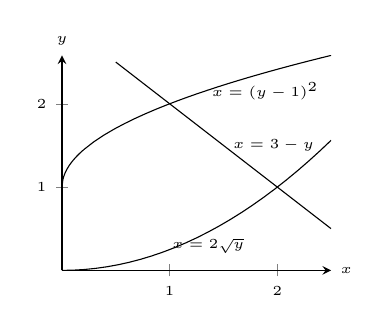
\begin{tikzpicture}[font=\tiny,declare function={fa(\x)=1+sqrt(\x); fb(\x)=3-\x; fc(\x)=x^2/4;}]
\begin{axis}[width=5cm,axis lines=middle,xlabel={$x$},ylabel={$y$},xlabel style={at={(current axis.right of origin)},anchor=west},ylabel style={at={(current axis.above origin)},anchor=south},xtick={1,2},ytick={1,2}]
\addplot[domain=0:0.2]{fa(x)};
\addplot[domain=0.2:2.5]{fa(x)}node[pos=0.75,below]{$x=(y-1)^2$};
\addplot[domain=0.5:2.5]{fb(x)}node[pos=0.5,right]{$x=3-y$};
\addplot[domain=0:2.5]{fc(x)}node[pos=0.5,below,xshift=-0.5ex]{$x=2\sqrt{y}$};
\end{axis}
\end{tikzpicture}
\caption{خطہ برائے سوال \حوالہ{سوال_تکمل_استعمال_رقبہ_محیط_خاکہ_الف}}
\label{شکل_سوال_تکمل_استعمال_رقبہ_محیط_خاکہ_الف}
\end{minipage}\hfill
\begin{minipage}{0.3\textwidth}
\centering
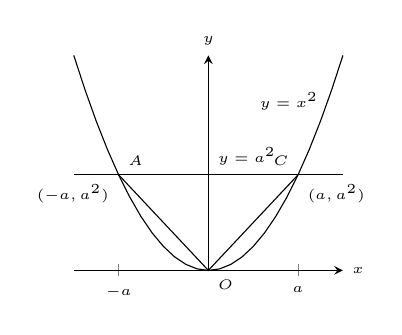
\begin{tikzpicture}[font=\tiny,declare function={fa(\x)=\x^2; fb(\x)=4;}]
\begin{axis}[clip=false,width=5cm,axis lines=middle,xlabel={$x$},ylabel={$y$},xlabel style={at={(current axis.right of origin)},anchor=west},ylabel style={at={(current axis.above origin)},anchor=south},xtick={-2,2},xticklabels={$-a$,$a$},ytick={\empty}]
\addplot[domain=-3:3]{fa(x)}node[pos=0.9,left]{$y=x^2$};
\addplot[domain=-3:3]{fb(x)}node[pos=0.5,above right]{$y=a^2$};
\draw(axis cs:-2,4)node[below left]{$(-a,a^2)$}node[above right]{$A$}--(axis cs:0,0)node[below right]{$O$}--(axis cs:2,4)node[below right]{$(a,a^2)$}node[above left]{$C$};
\end{axis}
\end{tikzpicture}
\caption{خطہ برائے سوال \حوالہ{سوال_تکمل_استعمال_رقبہ_محیط_خاکہ_ب}}
\label{شکل_سوال_تکمل_استعمال_رقبہ_محیط_خاکہ_ب}
\end{minipage}\hfill
\begin{minipage}{0.3\textwidth}
\centering
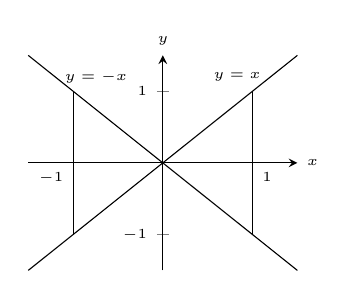
\begin{tikzpicture}[font=\tiny,declare function={fa(\x)=\x; fb(\x)=-\x;}]
\begin{axis}[clip=false,width=5cm,axis lines=middle,xlabel={$x$},ylabel={$y$},xlabel style={at={(current axis.right of origin)},anchor=west},ylabel style={at={(current axis.above origin)},anchor=south},xtick={-1,1},xticklabels={,},ytick={-1,1}]
\addplot[domain=-1.5:1.5]{fa(x)}node[pos=0.9,left]{$y=x$};
\addplot[domain=-1.5:1.5]{fb(x)}node[pos=0.1,right]{$y=-x$};
\draw(axis cs:-1,-1)--(axis cs:-1,1)  (axis cs:1,-1)--(axis cs:1,1);
\draw(axis cs:-1,0)node[below left,font=\tiny]{$-1$};
\draw(axis cs:1,0)node[below right,font=\tiny]{$1$};
\end{axis}
\end{tikzpicture}
\caption{خطہ برائے سوال \حوالہ{سوال_تکمل_استعمال_رقبہ_محیط_خاکہ_پ}}
\label{شکل_سوال_تکمل_استعمال_رقبہ_محیط_خاکہ_پ}
\end{minipage}
\end{figure}
%
\ابتدا{سوال}
مثبت استمراری تفاعل \عددی{f} اور \عددی{a\le x\le b} پر \عددی{x} محور کے بیچ رقبہ \عددی{4} ہے۔ منحنی \عددی{y=f(x)} اور \عددی{y=2f(x)} کے بیچ رقبہ  \عددی{x=a} تا \عددی{x=b} رقبہ تلاش کریں۔
\انتہا{سوال}
%============================
\ابتدا{سوال}\شناخت{سوال_تکمل_استعمال_رقبہ_محیط_خاکہ_پ}
درج ذیل میں سے کونسا تکمل شکل \حوالہ{شکل_سوال_تکمل_استعمال_رقبہ_محیط_خاکہ_پ} میں دکھایا گیا رقبہ دیتا ہے؟ اپنے جواب کی وجہ پیش کریں۔
\begin{enumerate}[a.]
\item
$\int_{-1}^1(x-(-x))\dif x=\int_{-1}^12x\dif x$
\item
$\int_{-1}^1(-x-(x))\dif x=\int_{-1}^1-2x\dif x$
\end{enumerate}
جواب:\quad
کوئی نہیں
\انتہا{سوال}
%===========================
\ابتدا{سوال}
کیا استمراری تفاعل \عددی{y=f(x)} اور \عددی{y=g(x)} اور انتصابی لکیروں \عددی{x=a} اور \عددی{x=b} جہاں \عددی{a<b} ہے کے بیچ رقبہ درج ذیل دیتا ہے؟ درست، کبھی کبھار درست یا کبھی نہیں؟ اپنے جواب کی وجہ پیش کریں۔
\begin{align*}
\int_a^b[f(x)-g(x)]\dif x
\end{align*}
\انتہا{سوال}
%====================
\موٹا{کمپیوٹر کا استعمال}\\
سوال \حوالہ{سوال_تکمل_استعمال_کمپیوٹر_الف} تا سوال \حوالہ{سوال_تکمل_استعمال_کمپیوٹر_ب} میں مستوی میں منحنیات کے بیچ رقبہ تلاش کریں۔ جہاں منحنیات کے نقاط تقاطع تلاش کرنا دشوار ہو وہاں کمپیوٹر کا سہارا لیتے ہوئے درج ذیل اقدام سرانجام دیں۔
\begin{enumerate}[a.]
\item
منحنیات کو ایک ساتھ ترسیم کرتے ہوئے خطہ کی عمومی صورت دیکھیں اور نقاط تقاطع کی تعداد جانیں۔
\item
نقاط تقاطع کو اعدادی تراکیب سے تلاش کریں۔
\item
یک بعد دیگرے جوڑی نقاط تقاطع کے بیچ \عددی{\abs{f(x)-g(x)}} کا تکمل حل کریں۔
\item
جزو-ج میں تکمل کی حاصل قیمتوں کا مجموعہ لیں۔
\end{enumerate}

\ابتدا{سوال}\شناخت{سوال_تکمل_استعمال_کمپیوٹر_الف}
$f(x)=\tfrac{x^3}{3}-\tfrac{x^2}{2}-2x+\tfrac{1}{3},\quad g(x)=x-1$
\انتہا{سوال}
%======================
\ابتدا{سوال}
$f(x)=\tfrac{x^4}{2}-3x^3+10,\quad g(x)=8-12x$
\انتہا{سوال}
%===========================
\ابتدا{سوال}
$f(x)=x+\sin(2x),\quad g(x)=x^3$
\انتہا{سوال}
%===========================
\ابتدا{سوال}\شناخت{سوال_تکمل_استعمال_کمپیوٹر_ب}
$f(x)=x^2\cos x,\quad g(x)=x^3-x$
\انتہا{سوال}
%===========================

\حصہ{ٹکیاں کاٹ کر حجم کی تلاش}
قوسی سرحد کے خطوں کے رقبہ عمودی تراش سے بیلنی حجم معلوم کرنے کے لئے رقبہ عمودی تراش کو بیلن کے قد سے ضرب دیا جاتا ہے۔ اس طرز کے بیلنی حجم سے دیگر اشکال کے خطوں کا حجم تلاش کیا جا سکتا ہے۔

\جزوحصہء{ٹکیاں}
فرض کریں ہم شکل \حوالہ{شکل_تکمل_استعمال_ٹکیاں} میں دکھائے گئے ٹھوس جسم کا حجم دریافت کرنا چاہتے ہیں۔ بند وقفہ \عددی{[a,b]} کے ہر نقطہ \عددی{x} پر جسم کا عمودی تراش خطہ \عددی{R(x)} ہے جس کا رقبہ \عددی{S(x)} ہے۔ یوں \عددی{S} متغیر \عددی{x} کا حقیقی قیمت تفاعل ہو گا جو \عددی{x} کا استمراری تفاعل بھی ہو گا۔اس کو استعمال کرتے ہوئے جسم کے حجم کی تعریف پیش کی جا سکتی ہے جس کو درج ذیل طریقہ سے حاصل کیا جا سکتا ہے۔
\begin{figure}
\centering
\begin{minipage}{0.45\textwidth}
\centering
\begin{tikzpicture}
\draw[](2,0) circle (0.25cm and 1cm);
\draw([shift={(90:0.25cm and 0.75cm)}]0,-0.5cm) arc  (90:270:0.25cm and 0.5cm)coordinate[pos=0](t)coordinate[pos=1](b);
\draw(2,1) to [out=180,in=-20](t);
\draw(2,-1) to [out=200,in=45](b);
\fill[lgray](1,-0.13) circle (0.25cm and 0.65cm);
\draw[]([shift={(90:0.25cm and 0.65cm)}]1,-0.13) arc (90:270:0.25cm and 0.65cm);
\draw[dashed]([shift={(-90:0.25cm and 0.65cm)}]1,-0.13) arc (-90:90:0.25cm and 0.65cm);
\draw[-latex](-0.5,-1.5)--(2.5,-1.5)node[right]{$x$};
\draw(0,-1.5)node[below]{$a$}--++(0,0.1)  (2,-1.5)node[below]{$b$}--++(0,0.1)  (1,-1.5)node[below]{$x$};
\draw(1,0.3)--++(60:1.5)node[above,align=left]{\RL{خطہ عمودی تراش $R(x)$}\\  \RL{رقبہ عمودی تراش $S(x)$}};
\end{tikzpicture}
\caption{عمودی تراش $R(x)$ کا رقبہ $S(x)$ متغیر $x$ کا استمراری تفاعل ہونے کی صورت میں ہم ٹھوس جسم کا حجم $x=a$ تا $x=b$ تفاعل $S(x)$ کا تکمل لے کر حاصل کر سکتے ہیں۔}
\label{شکل_تکمل_استعمال_ٹکیاں}
\end{minipage}\hfill
\begin{minipage}{0.45\textwidth}
\centering
\begin{tikzpicture}
\pgfmathsetmacro{\len}{2}
\pgfmathsetmacro{\la}{1.5}
\pgfmathsetmacro{\lb}{3.25}
\pgfmathsetmacro{\anga}{20}
\pgfmathsetmacro{\angb}{70}
\fill[llgray,fill opacity=0.5](0,-1.5)--++(\anga:-\la)--++(70:\lb)--++(\anga:\la)--++(70:-\lb);
\fill[white] (\len,1)--(0,1) ([shift={(90:0.25cm and 1cm)}]0,0) arc (90:270:0.25cm and 1cm)--(\len,-1)--(\len,1);
\draw([shift={(90:0.25cm and 1cm)}]0,0) arc (90:270:0.25cm and 1cm);
\draw(\len,0) circle (0.25cm and 1cm);
\draw[name path=up](0,1)--(\len,1)coordinate[pos=0.5](kcyln);
\draw[name path=lo](0,-1)--(\len,-1);
\draw([shift={(90:0.25cm and 0.75cm)}]0.25,0) arc (90:270:0.25cm and 0.75cm);
\draw(0.25,0.75)to [out=0,in=180](\len,1)  (0.25,-0.75) to [out=0,in=180](\len,-1);
\draw[name path=leftS](0,-1.5)coordinate(LB)--++(\anga:-\la)--++(\angb:\lb)coordinate(kSa)--++(\anga:\la)coordinate(LT);
\path[name path=aa](LT)--++(\angb:-\lb);
\path[name path=bb](LB)--++(\angb:\lb);
\draw[name intersections={of=aa and up}](LT)--(intersection-1);
\draw[name intersections={of=bb and lo}](LB)--(intersection-1);
\draw[name path=rightS,fill=llgray,fill opacity=0.5](\len,-1.5)--++(\anga:-\la)--++(\angb:\lb)--++(\anga:\la)coordinate(kSb)--++(\angb:-\lb);
\draw(kSa)node[left]{\RL{$x_{k-1}$ پر سطح}};
\draw(kSb)node[right]{\RL{$x_{k}$ پر سطح}};
\draw(kcyln)--++(45:1)node[above,xshift=1ex]{\RL{تخمینی بیلن}};
\path[name path=axisa](0,-1.5)++(\anga:-\la/2)coordinate(ksolid)node[below]{$x_{k-1}$}++(-0.1,0)--++(-1,0);
\path[name path=axisb](\len,-1.5)++(\anga:-\la/2)coordinate(ksolida)node[below]{$x_k$}++(-0.1,0)--++(-1,0);
\draw[dashed,name intersections={of=axisa and leftS}] (0,-1.5)++(\anga:-\la/2)--(intersection-1);
\draw(intersection-1)--++(-1,0);
\draw[dashed,name intersections={of=axisb and rightS}] (\len,-1.5)++(\anga:-\la/2)--(intersection-1);
\draw(intersection-1)--(ksolid);
\draw[-stealth](ksolida)--++(1,0)node[right]{$x$};
\draw[fill=lgray](\len,0) circle (0.25cm and 1cm);
\draw(\len,0.75)--++(-20:1cm)node[right,align=right]{\RL{بیلن کا قاعدہ}\\ \RL{ خطہ $R(x_k)$ ہے}};
\end{tikzpicture}
\caption{سطح $x_{k-1}$ اور $x_k$ کے بیچ ٹکیا کو بڑا کر کے دکھایا گیا ہے اور ساتھ ہی تخمینی بیلن بھی دکھایا گیا ہے۔}
\label{شکل_تکمل_استعمال_تخمینی_بیلن}
\end{minipage}
\end{figure}

ہم \عددی{x} محور کے لحاظ سے وقفہ \عددی{[a,b]} کی خانہ بندی کر کے جسم کو خانہ بند نقطوں پر \عددی{x} محور کے عمودی، سطحوں سے مولی کی طرح  چپٹا ٹکڑے کرتے ہوئے جسم کی ٹکیاں بناتے ہیں۔یوں نقطہ \عددی{x_{k-1}} اور \عددی{x_k} پر سطحوں کے بیچ \عددی{k} ویں ٹکیا کا حجم تقریباً اس بیلن جتنا ہو گا جو ان سطحوں کے بیچ پایا جاتا ہے اور جس کا عمودی تراش خطہ \عددی{R(x_k)} ہے (شکل \حوالہ{شکل_تکمل_استعمال_تخمینی_بیلن})۔ اس بیلن کا حجم درج ذیل ہو گا۔
\begin{align*}
H_k&=\text{\RL{رقبہ قاعدہ}}\times \text{قد}\\
&=S(x_k)\times (\text{\RL{$x_{k-1}$ اور $x_k$ کے بیچ فاصلہ}})\\
&=S(x_k)\Delta x_k
\end{align*}
اس طرح تمام چھوٹے بیلنوں کے حجم کا مجموعہ تخمیناً ٹھوس جسم کے حجم کے برابر ہو گا:
\begin{align*}
\sum_{k=1}^nS(x_k)\Delta x_k
\end{align*} 
یہ وقفہ \عددی{[a,b]} پر تفاعل \عددی{S(x)} کا ریمان مجموعہ ہے۔ ہم توقع کرتے ہیں۔ کہ جیسے جیسے \عددی{[a,b]} کی خانہ بندی کا معیار صفر تک پہنچے ویسے ویسے یہ مجموعے اصل حجم کی بہتر سے بہتر عکاسی کریں گے۔ یوں ٹھوس جسم کے حجم کی تعریف ان مجموعوں کا تحدیدی تکمل ہو گا۔

\ابتدا{تعریف} 
ایسا ٹھوس جسم جس کا رقبہ عمودی تراش \عددی{S(x)} قابل تکمل تفاعل ہو،  کا \عددی{x=a} سے \عددی{x=b} تک حجم  \عددی{x=a} تا \عددی{x=b} تفاعل \عددی{S} کا تکمل ہو گا:
\begin{align}\label{مساوات_تکمل_استعمال_تعریف_حجم_الف}
H=\int_a^b S(x)\dif x
\end{align}
\انتہا{تعریف}
%======================

مساوات \حوالہ{مساوات_تکمل_استعمال_تعریف_حجم_الف} استعمال کرنے کے لئے درج ذیل تین اقدام کرنے ہوں گے۔

\موٹا{ٹھوس جسم کی ٹکیوں سے حجم کی تلاش}\\
\begin{enumerate}[1.]
\item
ٹھوس جسم  اور اس کے نمائندہ عمودی تراش کا خاکہ کھینچیں۔
\item
 رقبہ عمودی تراش \عددی{S(x)} کا کلیہ اخذ کریں۔
\item
تکمل کا زیریں اور بالائی حد تلاش کریں۔
\item
حجم معلوم کرنے کی خاطر \عددی{S(x)} کا تکمل حل کریں۔
\end{enumerate}

\ابتدا{مثال}\شناخت{مثال_تکمل_استعمال_اہرام_چکور_قاعدہ}
ایک اہرام کا قد \عددی{\SI{3}{\meter}} اور اس کے چکور بنیاد کا ضلع \عددی{\SI{3}{\meter}} ہے۔ اہرام کی چوٹی سے \عددی{x} میٹر نیچے اہرام کا رقبہ عمودی تراش چکور ہو گا جس کا ضلع \عددی{x} میٹر ہو گا۔ اس اہرام کا حجم تلاش کریں۔

حل:\quad
\موٹا{پہلا قدم:}\quad
\ترچھا{خاکہ۔}\quad
ہم اہرام کی چوٹی کو مبدا پر رکھ کر اہرام کو \عددی{x} محور پر لیٹا ہوا بنا کر نمائندہ رقبہ عمودی تراش بناتے ہیں (شکل \حوالہ{شکل_مثال_تکمل_استعمال_اہرام_چکور_قاعدہ})۔\\
\موٹا{دوسرا قدم:}\quad
\ترچھا{کلیہ برائے \عددی{S(x)}۔}
\quad
چونکہ چکور رقبہ عمودی تراش کا ضلع \عددی{x} میٹر ہے لہٰذا اس کا رقبہ عمودی تراش \عددی{S(x)=x^2} ہو گا۔\\
\موٹا{تیسرا قدم:}\quad
\ترچھا{تکمل کے حد۔}\quad
چکور \عددی{x=0} تا \عددی{x=3} پائے جاتے ہیں لہٰذا \عددی{a=0} اور \عددی{b=3} ہوں گے۔\\
\موٹا{چوتھا قدم:}\quad \ترچھا{حجم۔}
\begin{align*}
H=\int_a^bS(x)\dif x=\int_0^3x^2\dif x=\left.\tfrac{x^3}{3}\right\vert_0^3=9
\end{align*}
یوں اہرام کا حجم \عددی{\SI{9}{\meter\cubed}} ہو گا۔
\انتہا{مثال}
%==========================
\begin{figure}
\centering
\begin{minipage}{0.45\textwidth}
\centering
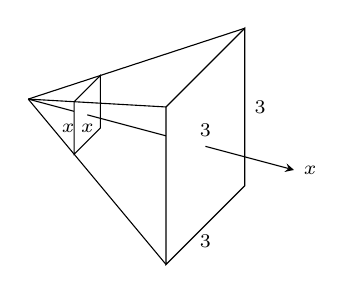
\begin{tikzpicture}[font=\scriptsize,x={(0.75cm,-0.2cm)},y={(0cm,1cm)},z={(-0.5cm,-0.5cm)}]
\pgfmathsetmacro{\la}{2/3}
\pgfmathsetmacro{\lb}{2}
\draw(0,0,0)--(1,0,0);
\draw[fill=white](1,\la/2,\la/2)--++(0,-\la,0)node[pos=0.5,xshift=-0.5ex]{$x$}--++(0,0,-\la)--++(0,\la,0)--++(0,0,\la);
\draw(1,0,0)node[below]{$x$}--(3,0,0);
\draw[fill=white](3,\lb/2,\lb/2)--++(0,-\lb,0)--++(0,0,-\lb)node[pos=0.5,below]{$3$}--++(0,\lb,0)node[pos=0.5,right]{$3$}--++(0,0,\lb);
\draw[-stealth](3,0,0)node[above]{$3$}--(4.5,0,0)node[right]{$x$};
\draw(0,0,0)--(3,-\lb/2,\lb/2);
\draw(0,0,0)--(3,\lb/2,\lb/2);
\draw(0,0,0)--(3,\lb/2,-\lb/2);
%\draw(0,0,0)--(3,-\lb/2,-\lb/2);
\end{tikzpicture}
\caption{اہرام (مثال \حوالہ{مثال_تکمل_استعمال_اہرام_چکور_قاعدہ}) }
\label{شکل_مثال_تکمل_استعمال_اہرام_چکور_قاعدہ}
\end{minipage}\hfill
\begin{minipage}{0.45\textwidth}
\centering
\begin{tikzpicture}[scale=1.5,x={(0.75cm,0.2cm)},y={(-0.5cm,0.5cm)},z={(0,1cm)},font=\scriptsize]
\pgfmathsetmacro{\la}{1.5}
\draw([shift={(-90:\la)}]0,0,0) arc (-90:90:\la)coordinate[pos=0.3](ka)coordinate[pos=0.15](kSa)coordinate[pos=0.85](kEa);
\begin{scope}[x={(0.75cm,0.75cm)},y={(-0.5cm,0.5cm)},z={(0,1cm)}]
\draw(0,-1.25*\la)--(0,1.25*\la);
\draw([shift={(-90:\la)}]0,0,0) arc (-90:90:\la)coordinate[pos=0.3](kb)coordinate[pos=0.15](kSb)coordinate[pos=0.85](kEb);
\end{scope}
\draw[name path=edgeR](ka)--(kb);
\draw(kSa)--(kSb)--(kEb)coordinate[pos=0.5](kC)--(kEa)--(kSa)coordinate[pos=0.5](kCC);
\draw(0,0)--(kC)--(kCC)node[pos=0.5,shift={(0.1cm,0)}]{$x$};
\draw($(0,0)!0.5!(kCC)$)node[below]{$x$};
\draw(kSa)++(0,-0.1)--++(-45:0.5)node[right]{$(x,\sqrt{9-x^2})$};
\draw[dashed](0,0)--(kEa)node[pos=0.6,left]{$3$};
\path[name path=xaxis](-0.2*\la,0)--(1.75*\la,0);
\draw(0,0)--(kCC);
\draw[-stealth,name intersections={of=edgeR and xaxis}] (intersection-1)node[below right]{$3$}--(1.75*\la,0)node[right]{$x$};
\draw[-stealth](0,-1.25*\la)--(0,1.5*\la)node[above]{$y$};
\end{tikzpicture}
\caption{قوسی پچر (مثال \حوالہ{مثال_تکمل_استعمال_قوسی_پچر})}
\label{شکل_مثال_تکمل_استعمال_قوسی_پچر}
\end{minipage}
\end{figure}
\ابتدا{مثال}\شناخت{مثال_تکمل_استعمال_قوسی_پچر}
رداس \عددی{3} کے بیلن کو دو مستوی سے کاٹ کر قوسی پچر بنایا جاتا ہے۔ایک مستوی بیلن کے محور کا عمودی ہے جبکہ دوسرا مستوی پہلے مستوی کو بیلن کے وسط پر \عددی{45^{\circ}} سے قطع کرتا ہے۔ پچر کا حجم تلاش کریں۔

حل:\quad
\موٹا{پہلا قدم:} \quad \ترچھا{خاکہ۔}\quad
ہم پچر اور نمائندہ عمودی تراش کا خاکہ بناتے ہیں (شکل \حوالہ{شکل_مثال_تکمل_استعمال_قوسی_پچر})۔ عمودی تراش \عددی{x} محور کے عمودی ہے۔\\
\موٹا{دوسرا قدم:}\quad \ترچھا{کلیہ برائے \عددی{S(x)}۔}
\quad
نقطہ \عددی{x} پر مستطیل عمودی تراش کا رقبہ درج ذیل ہو گا۔
\begin{align*}
S(x)=(\text{قد})(\text{چوڑائی})=(x)(2\sqrt{9-x^2})=2x\sqrt{9-x^2}
\end{align*}
\موٹا{تیسرا قدم:}\quad
\ترچھا{تکمل کے حد۔}\quad
مستطیل \عددی{x=0} تا \عددی{x=3} پائے جاتے ہیں۔\\
\موٹا{چوتھا قدم:}\quad \ترچھا{حجم۔}
درج ذیل میں \عددی{u=9-x^2} لہٰذا \عددی{\dif u=-2x\dif x} لے کر تکمل حاصل کریں۔
\begin{align*}
H=\int_a^bS(x)\dif x&=\int_0^32x\sqrt{9-x^2}\dif x\\
&=\left.-\frac{2}{3}(9-x^2)^{3/2}\right\vert_0^3\\
&=0+\frac{2}{3}(9)^{3/2}\\
&=18
\end{align*}
\انتہا{مثال}
%========================

\ابتدا{مثال}\شناخت{مثال_تکمل_استعمال_مسئلہ_کولئیرے_ٹھوس}\ترچھا{مسئلہ کوالئیرے}\حاشیہد{اطالوی ریاضی دان بوناونتورا کوالئیرے [1598-1647]}
محور \عددی{x} پر پڑے ہوئے ایسے دو اجسام جن کا ہر \عددی{x} پر رقبہ عمودی تراش ایک دوسرے جیسا ہو کا حجم بھی ایک دوسرے جیسا ہو گا۔ یہ حقیقت  مساوات \حوالہ{مساوات_تکمل_استعمال_تعریف_حجم_الف} سے صاف ظاہر ہے چونکہ دونوں اجسام کا رقبہ عمودی تراش تفاعل \عددی{S(x)} ایک دوسرے جیسا ہے (شکل \حوالہ{شکل_مثال_تکمل_استعمال_مسئلہ_کولئیرے_ٹھوس})۔
\انتہا{مثال}
%===========================
\begin{figure}
\centering
\begin{tikzpicture}
\pgfmathsetmacro{\la}{1}
\pgfmathsetmacro{\lb}{0.25}
\pgfmathsetmacro{\xx}{0.75}
\pgfmathsetmacro{\h}{2}
\pgfmathsetmacro{\xb}{7.5*\la}
\pgfmathsetmacro{\yb}{1*\la}
\pgfmathsetmacro{\ang}{40}
\draw(0,0) circle (\la cm and \lb cm);
\draw([shift={(-180:\la cm and \lb cm)}]\xx,-\h) arc (-180:0:\la cm and \lb cm);
\draw[name path=Lr](\la,0) to [out=-90,in=90] coordinate[pos=0.5](Lmr)(\xx+1,-\h);
\draw[name path=Ll](-\la,0) to [out=-90,in=90] coordinate[pos=0.5](Lml)(\xx-1,-\h);
\fill[white](-2.5*\la,-2/3*\h)--++(\xb,0)--++(\ang:0.5*\yb)--++(-\xb,0)--++(\ang:-0.5*\yb);
\draw([shift={(-180:\la cm and \lb cm)}]$(Lml)!0.5!(Lmr)$) arc (-180:0:\la cm and \lb cm);
\draw[dashed]([shift={(0:\la cm and \lb cm)}]$(Lml)!0.5!(Lmr)$) arc (0:180:\la cm and \lb cm);
\begin{scope}[xshift={3.5*\la cm}]
\draw(0,0) circle (\la cm and \lb cm);
\draw([shift={(-180:\la cm and \lb cm)}]0,-\h) arc (-180:0:\la cm and \lb cm);
\draw[name path=Rr](\la,0)--(\la,-\h)coordinate[pos=0.5](Rmr);
\draw[name path=Rl](-\la,0)--(-\la,-\h)coordinate[pos=0.5](Rml);
\fill[white](-2.5*\la,-2/3*\h)--++(\xb,0)--++(\ang:0.5*\yb)--++(-\xb,0)--++(\ang:-0.5*\yb);
\draw([shift={(-180:\la cm and \lb cm)}]$(Rml)!0.5!(Rmr)$) arc (-180:0:\la cm and \lb cm);
\draw[dashed]([shift={(0:\la cm and \lb cm)}]$(Rml)!0.5!(Rmr)$) arc (0:180:\la cm and \lb cm);
\path[name path=back](-2*\la,-2/3*\h)++(\ang:\yb)--++(\xb,0);
\draw[name intersections={of=back and Rr,by=aa}] (aa)--++(1.75,0);
\end{scope}
\path[name path=back](-2*\la,-2/3*\h)++(\ang:\yb)--++(\xb,0);
\draw(-2*\la,-2/3*\h)--++(\xb,0)--++(\ang:\yb);
\draw(-2*\la,-2/3*\h)--++(\ang:\yb);
\draw(-2*\la,-1.3*\h)++(\ang:\yb/2)--++(0,1.5*\h);
\draw(-2*\la,-1.2*\h)++(\ang:\yb/2)node[left]{$a$}--++(0.1,0);
\draw(-2*\la,-0.2*\h)++(\ang:\yb/2)node[left]{$b$}--++(0.1,0);
\fill[white](-2*\la,-2/3*\h)++(\ang:\yb)--++(\ang:-\yb)--++(1,0)--cycle;
\draw[name intersections={of=back and Ll,by=aa},name intersections={of=back and Lr,by=bb}] (-2*\la,-2/3*\h)++(\ang:\yb)--(aa) (bb)--++(1.32,0);
\end{tikzpicture}
\caption{ان اجسام کا حجم ایک دوسرے جیسا ہے۔ آپ سکوں کو ایک دوسرے کے اوپر رکھ کر اس کو ثابت کر سکتے ہیں۔}
\label{شکل_مثال_تکمل_استعمال_مسئلہ_کولئیرے_ٹھوس}
\end{figure}

\حصہء{سوالات}
\موٹا{رقبہ عمودی تراش}\\
سوال \حوالہ{سوال_تکمل_استعمال_رقبہ_عمودی_تراش_الف} اور سوال \حوالہ{سوال_تکمل_استعمال_رقبہ_عمودی_تراش_ب} میں \عددی{x} محور کے عمودی، ٹھوس جسم کے، رقبہ عمودی تراش \عددی{S(x)} کا کلیہ اخذ کریں۔ 

\ابتدا{سوال}\شناخت{سوال_تکمل_استعمال_رقبہ_عمودی_تراش_الف}
ایک ٹھوس جسم  \عددی{x=-1} اور \عددی{x=1} پر \عددی{x} محور  کے عمودی سطحوں کے بیچ پایا جاتا ہے۔  \عددی{x} محور کے عمودی جسم  کے رقبہ عمودی تراش نصف دائرہ \عددی{y=-\sqrt{1-x^2}} اور نصف دائرہ \عددی{y=\sqrt{1-x^2}} کے بیچ پائے جاتے ہیں ۔ 
\begin{enumerate}[a.]
\item
عمودی تراش دائری اقراص ہیں جن کے قطر \عددی{xy} مستوی میں ہیں (شکل \حوالہ{شکل_سوال_تکمل_استعمال_رقبہ_عمودی_تراش_الف}-ا)۔
\item
عمودی تراش چکور ہیں جن کے قاعدے \عددی{xy} مستوی میں ہیں (شکل \حوالہ{شکل_سوال_تکمل_استعمال_رقبہ_عمودی_تراش_الف}-ب)۔
\item
عمودی تراش چکور ہیں جن کے وتر \عددی{xy} مستوی میں ہیں۔ چکور کے وتر کی لمبائی چکور کے ضلع کے \عددی{\sqrt{2}} گنّا ہوتی ہے (شکل \حوالہ{شکل_سوال_تکمل_استعمال_رقبہ_عمودی_تراش_الف}-ج)۔
\item
عمودی تراش مساوی الاضلاع مثلث ہیں جن کے قاعدے \عددی{xy} مستوی میں ہیں (شکل \حوالہ{شکل_سوال_تکمل_استعمال_رقبہ_عمودی_تراش_الف}-د)۔
\end{enumerate}
جواب:\quad
(ا) \عددی{S(x)=\pi(1-x^2)}، (ب) \عددی{S(x)=4(1-x^2)}،\\ (ج) \عددی{S(x)=2(1-x^2)}، (د) \عددی{S(x)=\sqrt{3}(1-x^2)}
\انتہا{سوال}
%======================
\begin{figure}
\centering
\begin{subfigure}{0.22\textwidth}
\centering
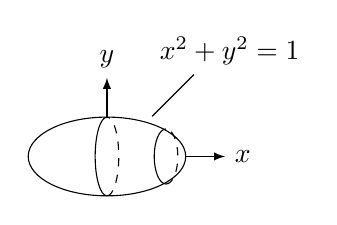
\begin{tikzpicture}
\pgfmathsetmacro{\ang}{120}
\pgfmathsetmacro{\la}{0.4}
\pgfmathsetmacro{\lb}{0.8}
\draw[-latex] (1,0)--++(0.5,0)node[right]{$x$};
\draw[-latex](0,0.5)--++(0,0.5)node[above]{$y$};
\draw([shift={(0:1cm and 0.5cm)}]0,0) arc (0:360:1cm and 0.5cm)coordinate[pos=0.1](ka)coordinate[pos=0.9](kb);
\draw([shift={(90:0.15cm and 0.35cm)}]0.75,0) arc (90:270:0.15 cm and 0.35cm);
\draw[dashed]([shift={(-90:0.15cm and 0.35cm)}]0.75,0) arc (-90:90:0.15 cm and 0.35cm);
\draw([shift={(90:0.15cm and 0.5cm)}]0,0) arc (90:270:0.15 cm and 0.5cm);
\draw[dashed]([shift={(-90:0.15cm and 0.5cm)}]0,0) arc (-90:90:0.15 cm and 0.5cm);
\draw(55:1cm and 0.5cm)++(0,0.1)--++(45:0.75)node[above,xshift=3ex]{$x^2+y^2=1$};
\end{tikzpicture}
\caption{}
\end{subfigure}\hfill
\begin{subfigure}{0.22\textwidth}
\centering
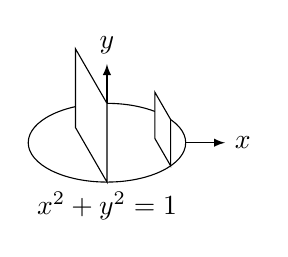
\begin{tikzpicture}
\pgfmathsetmacro{\ang}{120}
\pgfmathsetmacro{\la}{0.4}
\pgfmathsetmacro{\lb}{0.8}
\draw[-latex] (1,0)--++(0.5,0)node[right]{$x$};
\draw[-latex](0,0.5)--++(0,0.5)node[above]{$y$};
\draw([shift={(0:1cm and 0.5cm)}]0,0) arc (0:360:1cm and 0.5cm)coordinate[pos=0.1](ka)coordinate[pos=0.9](kb)node[pos=0.75,below]{$x^2+y^2=1$};
\draw[fill=white](ka)--(kb)--++(\ang:\la)coordinate(ta) (ka)--++(\ang:\la)coordinate(tb)--(ta);
\path([shift={(0:1cm and 0.5cm)}]0,0) arc (0:360:1cm and 0.5cm)coordinate[pos=0.25](ka)coordinate[pos=0.75](kb);
\draw[fill=white](ka)--(kb)--++(\ang:\lb)coordinate(ta) (ka)--++(\ang:\lb)coordinate(tb)--(ta);
\end{tikzpicture}
\caption{}
\end{subfigure}\hfill
\begin{subfigure}{0.22\textwidth}
\centering
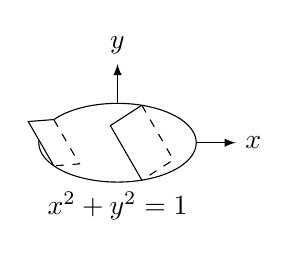
\begin{tikzpicture}
\pgfmathsetmacro{\ang}{120}
\pgfmathsetmacro{\la}{0.65}
\pgfmathsetmacro{\lb}{0.8}
\draw[-latex] (1,0)--++(0.5,0)node[right]{$x$};
\draw[-latex](0,0.5)--++(0,0.5)node[above]{$y$};
\draw([shift={(0:1cm and 0.5cm)}]0,0) arc (0:360:1cm and 0.5cm)coordinate[pos=0.2](ka)coordinate[pos=0.8](kb)node[pos=0.75,below]{$x^2+y^2=1$};
\draw[](kb)--++(\ang:\lb)--(ka);
\draw[dashed](ka)--++(\ang:-\lb)--(kb);
\path([shift={(0:1cm and 0.5cm)}]0,0) arc (0:360:1cm and 0.5cm)coordinate[pos=0.4](ka)coordinate[pos=0.6](kb);
\fill[white](kb)--++(\ang:\la)--(ka)--(kb);
\draw[](kb)--++(\ang:\la)--(ka);
\draw[dashed](ka)--++(\ang:-\la)--(kb);
\end{tikzpicture}
\caption{}
\end{subfigure}\hfill
\begin{subfigure}{0.22\textwidth}
\centering
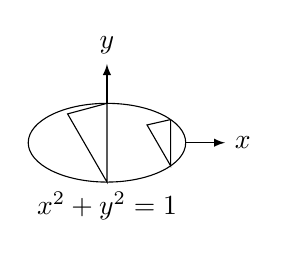
\begin{tikzpicture}
\pgfmathsetmacro{\ang}{120}
\pgfmathsetmacro{\la}{0.6}
\pgfmathsetmacro{\lb}{1}
\draw[-latex] (1,0)--++(0.5,0)node[right]{$x$};
\draw[-latex](0,0.5)--++(0,0.5)node[above]{$y$};
\draw([shift={(0:1cm and 0.5cm)}]0,0) arc (0:360:1cm and 0.5cm)coordinate[pos=0.1](ka)coordinate[pos=0.9](kb)node[pos=0.75,below]{$x^2+y^2=1$};
\draw[fill=white](ka)--(kb)--++(\ang:\la)--(ka);
\path([shift={(0:1cm and 0.5cm)}]0,0) arc (0:360:1cm and 0.5cm)coordinate[pos=0.25](ka)coordinate[pos=0.75](kb);
\draw[fill=white](ka)--(kb)--++(\ang:\lb)--(ka);
\end{tikzpicture}
\caption{}
\end{subfigure}\hfill
\caption{عمودی تراش برائے سوال \حوالہ{سوال_تکمل_استعمال_رقبہ_عمودی_تراش_الف}}
\label{شکل_سوال_تکمل_استعمال_رقبہ_عمودی_تراش_الف}
\end{figure}
%
\begin{figure}
\centering
\begin{subfigure}{0.45\textwidth}
\centering
\begin{tikzpicture}[y={0.5cm}]
\pgfmathsetmacro{\ra}{sqrt(2)/2}
\pgfmathsetmacro{\rb}{sqrt(1)/2}
\pgfmathsetmacro{\rc}{sqrt(1.5)/2}
\draw[-latex](2,0)node[below]{$4$}--(2.75,0)node[right]{$x$};
\draw[domain=0:0.5]plot({\x},{sqrt(\x)});
\draw[domain=0:0.5]plot({\x},{-sqrt(\x)});
\draw[domain=0.5:2]plot({\x},{sqrt(\x)});
\draw[domain=0.5:2]plot({\x},{-sqrt(\x)});
\draw[name path=Sr](2,0) circle (0.25cm and \ra cm);
\draw[name path=Sl](1,0) circle (0.2cm and \rb cm);
\path[name path=kaxis](0,0)--(2,0);
\draw[name intersections={of=kaxis and Sr, by=k},name intersections={of=kaxis and Sl}](1,0)--(k)  (-0.2,0)--(intersection-2);
\draw[-latex](0,-0.5)--(0,1)node[above]{$y$};
\draw(1.5,\rc)node[above,yshift=2ex]{$x=y^2$};
\end{tikzpicture}
\caption{}
\end{subfigure}\hfill
\begin{subfigure}{0.45\textwidth}
\centering
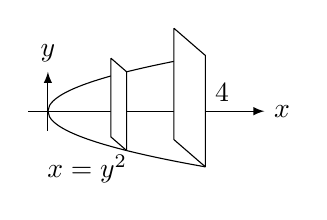
\begin{tikzpicture}[y={0.5cm}]
\pgfmathsetmacro{\ang}{120}
\pgfmathsetmacro{\la}{0.8}
\pgfmathsetmacro{\lb}{0.4}
\pgfmathsetmacro{\ra}{sqrt(2)/2}
\pgfmathsetmacro{\rb}{sqrt(1)/2}
\pgfmathsetmacro{\rc}{sqrt(1.5)/2}
\draw[-latex](-0.25,0)--(2.75,0)node[right]{$x$};
\draw(2,0)node[above right]{$4$};
\draw[-latex](0,-0.5)--(0,1)node[above]{$y$};
\draw[domain=0:0.5]plot({\x},{sqrt(\x)});
\draw[domain=0:0.5]plot({\x},{-sqrt(\x)});
\draw[domain=0.5:2]plot({\x},{sqrt(\x)});
\draw[domain=0.5:2]plot({\x},{-sqrt(\x)});
\draw[fill=white](2,{-sqrt(2)})--(2,{sqrt(2)})--++(\ang:\la)coordinate(t)  (2,{-sqrt(2)})--++(\ang:\la)--(t);
\draw[fill=white](1,{-sqrt(1)})--(1,{sqrt(1)})--++(\ang:\lb)coordinate(t)  (1,{-sqrt(1)})--++(\ang:\lb)--(t);
\draw(0.5,{-sqrt(0.5)})node[below,yshift=-0.5ex]{$x=y^2$};
\end{tikzpicture}
\caption{}
\end{subfigure}\hfill
\caption{عمودی تراش برائے سوال \حوالہ{سوال_تکمل_استعمال_رقبہ_عمودی_تراش_ب}}
\label{شکل_سوال_تکمل_استعمال_رقبہ_عمودی_تراش_ب}
\end{figure}

\ابتدا{سوال}\شناخت{سوال_تکمل_استعمال_رقبہ_عمودی_تراش_ب}
ایک ٹھوس جسم  \عددی{x=0} اور \عددی{x=4} پر  \عددی{x} محور  کے عمودی  سطحوں کے بیچ پایا جاتا ہے۔ \عددی{x} محور کے عمودی جسم  کے رقبہ عمودی تراش، قطع مکافی  \عددی{y=-\sqrt{x}} اور قطع مکافی \عددی{y=\sqrt{x}} کے بیچ پائے جاتے ہیں۔ 
\begin{enumerate}[a.]
\item
عمودی تراش دائری اقراص ہیں جن کے قطر \عددی{xy} مستوی میں ہیں (شکل \حوالہ{شکل_سوال_تکمل_استعمال_رقبہ_عمودی_تراش_ب}-ا)۔
\item
عمودی تراش چکور ہیں جن کے قاعدے \عددی{xy} مستوی میں ہیں (شکل \حوالہ{سوال_تکمل_استعمال_رقبہ_عمودی_تراش_ب}-ب)۔
\item
عمودی تراش چکور ہیں جن کے وتر \عددی{xy} مستوی میں ہیں۔
\item
عمودی تراش مساوی الاضلاع مثلث ہیں جن کے قاعدے \عددی{xy} مستوی میں ہیں۔
\end{enumerate}

\انتہا{سوال}
%====================
\موٹا{ٹکیوں سے حجم کی تلاش}\\
سوال \حوالہ{سوال_تکمل_استعمال_ٹھوس_جسم_حجم_الف} تا سوال \حوالہ{سوال_تکمل_استعمال_ٹھوس_جسم_حجم_ب} میں دیے گئے ٹھوس اجسام کے حجم تلاش کریں۔

\ابتدا{سوال}\شناخت{سوال_تکمل_استعمال_ٹھوس_جسم_حجم_الف}
ایک ٹھوس جسم \عددی{x=0} اور \عددی{x=4} پر  \عددی{x} محور کے عمودی سطحوں کے بیچ پایا جاتا ہے۔ جسم کے عمودی تراش کی صورت چکور ہے جو  \عددی{x} محور کے عمودی ہیں اور جن کے وتر قطع مکافی \عددی{y=-\sqrt{x}} سے قطع مکافی \عددی{y=\sqrt{x}} تک ہیں۔\\
جواب:\quad
$16$
\انتہا{سوال}
%========================
\ابتدا{سوال}
ایک ٹھوس جسم \عددی{x=-1} اور \عددی{x=1} پر  \عددی{x} محور کے عمودی سطحوں کے بیچ پایا جاتا ہے۔ جسم کے عمودی تراش \عددی{x} محور کے عمودی ہیں جن کے قطر دائری اقراص ہیں جو قطع مکافی \عددی{y=x^2} سے قطع مکافی \عددی{y=2-x^2} تک ہیں۔   
\انتہا{سوال}
%=====================
\ابتدا{سوال}
ایک ٹھوس جسم \عددی{x=-1} اور \عددی{x=1} پر  \عددی{x} محور کے عمودی سطحوں کے بیچ پایا جاتا ہے۔ جسم کے چکور عمودی تراش \عددی{x} محور کے عمودی ہیں جن کے قاعدہ کے کنارے نصف دائرہ \عددی{y=-\sqrt{1-x^2}} سے نصف دائرہ \عددی{y=\sqrt{1-x^2}} تک ہیں۔ \\
جواب:\quad
$\tfrac{16}{3}$  
\انتہا{سوال}
%======================
\ابتدا{سوال}
ایک ٹھوس جسم \عددی{x=-1} اور \عددی{x=1} پر  \عددی{x} محور کے عمودی سطحوں کے بیچ پایا جاتا ہے۔ جسم کے چکور عمودی تراش \عددی{x} محور کے عمودی ہیں جن کے وتر نصف دائرہ \عددی{y=-\sqrt{1-x^2}} سے نصف دائرہ \عددی{y=\sqrt{1-x^2}} تک ہیں۔ چکور کے وتر کی لمبائی چکور کے ضلع کے \عددی{\sqrt{2}} گنّا ہوتی ہے۔
\انتہا{سوال}
%======================
\ابتدا{سوال}\شناخت{سوال_تکمل_استعمال_شکل_دیا_گیا_ہے_الف}
ایک ٹھوس جسم کا قاعدہ منحنی \عددی{y=2\sqrt{\sin x}} اور \عددی{x} محور پر وقفہ \عددی{[0,\pi]}  کے بیچ پایا جاتا ہے۔ \عددی{x} محور کے عمودی عمودی تراش درج ذیل ہیں۔
\begin{enumerate}[a.]
\item
مساوی الاضلاع  مثلث جن کے قاعدے \عددی{x} محور سے منحنی تک ہیں (شکل \حوالہ{شکل_سوال_تکمل_استعمال_شکل_دیا_گیا_ہے_الف})۔
\item
انتصابی چکور جن کے قاعدے \عددی{x} محور سے منحنی تک ہیں۔
\end{enumerate}
جواب:\quad
(ا) \عددی{2\sqrt{3}}، (ب) \عددی{8}
\انتہا{سوال}
%=====================
\begin{figure}
\centering
\begin{minipage}{0.45\textwidth}
\centering
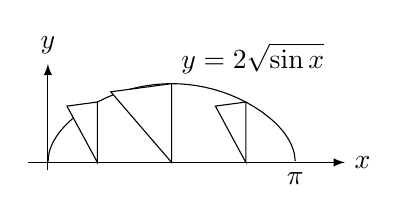
\begin{tikzpicture}[yscale=0.5]
\pgfmathsetmacro{\ang}{195}
\pgfmathsetmacro{\la}{0.4}
\pgfmathsetmacro{\lb}{0.8}
\draw[-latex](-0.25,0)--(1.2*pi,0)node[right]{$x$};
\draw[-latex](0,-0.2)--(0,2.5)node[above]{$y$};
\draw(pi,0)node[below]{$\pi$};
\draw[domain=0:pi/10] plot({\x},{2*sqrt(sin(deg(\x)))});
\draw[domain=0.9*pi:pi] plot({\x},{2*sqrt(sin(deg(\x)))});
\draw[domain=0.1*pi:0.9*pi] plot({\x},{2*sqrt(sin(deg(\x)))});
\draw[fill=white] (0.8*pi,{2*sqrt(sin(deg(0.8*pi)))})--++(\ang:\la)--(0.8*pi,0)--cycle;
\draw[fill=white] (0.5*pi,{2*sqrt(sin(deg(0.5*pi)))})--++(\ang:\lb)--(0.5*pi,0)--cycle;
\draw[fill=white] (0.2*pi,{2*sqrt(sin(deg(0.2*pi)))})--++(\ang:\la)--(0.2*pi,0)--cycle;
\draw(pi/2,{2*sqrt(sin(deg(0.5*pi)))})node[above right]{$y=2\sqrt{\sin x}$};
\end{tikzpicture}
\caption{عمودی تراش (سوال \حوالہ{سوال_تکمل_استعمال_شکل_دیا_گیا_ہے_الف})}
\label{شکل_سوال_تکمل_استعمال_شکل_دیا_گیا_ہے_الف}
\end{minipage}\hfill
\begin{minipage}{0.45\textwidth}
\centering
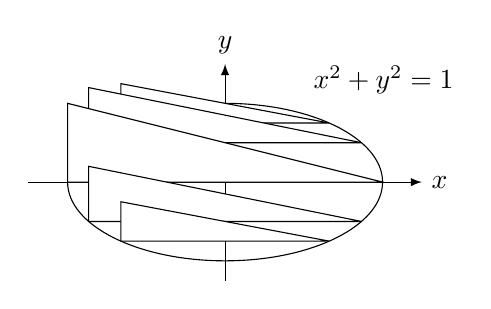
\begin{tikzpicture}[xscale=2]
\pgfmathsetmacro{\ang}{195}
\pgfmathsetmacro{\la}{1}
\pgfmathsetmacro{\lb}{0.7}
\pgfmathsetmacro{\lc}{0.5}
\pgfmathsetmacro{\aa}{sqrt(1-0^2)};
\pgfmathsetmacro{\bb}{sqrt(1-0.5^2)};
\pgfmathsetmacro{\cc}{sqrt(1-0.75^2)};
\draw[-latex](-1.25,0)--(1.25,0)node[right]{$x$};
\draw[-latex](0,-1.25)--(0,1.5)node[above]{$y$};
\draw(0,0) circle (1);
\draw[fill=white](\cc,0.75)--++(-2*\cc,0)--++(0,\lc)--cycle;
\draw[fill=white](\bb,0.5)--++(-2*\bb,0)--++(0,\lb)--cycle;
\draw[fill=white](\aa,0)--++(-2*\aa,0)--++(0,\la)--cycle;
\draw[fill=white](\bb,-0.5)--++(-2*\bb,0)--++(0,\lb)--cycle;
\draw[fill=white](\cc,-0.75)--++(-2*\cc,0)--++(0,\lc)--cycle;
\draw(0.5,1)node[above right]{$x^2+y^2=1$};
\end{tikzpicture}
\caption{عمودی تراش (سوال \حوالہ{سوال_تکمل_استعمال_شکل_دیا_گیا_ہے_ب})}
\label{شکل_سوال_تکمل_استعمال_شکل_دیا_گیا_ہے_ب}
\end{minipage}
\end{figure}
\ابتدا{سوال}
ایک ٹھوس جسم \عددی{x=-\tfrac{\pi}{3}} اور \عددی{x=\tfrac{\pi}{3}} پر  \عددی{x} محور کے عمودی سطحوں کے بیچ پایا جاتا ہے۔ جسم کے  عمودی تراش \عددی{x} محور کے عمودی ہیں جن کی خواص درج ذیل ہیں۔
\begin{enumerate}[a.]
\item
دائری اقراص جن کے قطر \عددی{y=\tan x} سے \عددی{y=\sec x} تک ہیں۔
\item
انتصابی چکور کن کے قاعدے  \عددی{y=\tan x} سے \عددی{y=\sec x} تک ہیں۔
\end{enumerate}
\انتہا{سوال}
%=====================
\ابتدا{سوال}
ایک ٹھوس جسم \عددی{y=0} اور \عددی{y=2} پر  \عددی{y} محور کے عمودی سطحوں کے بیچ پایا جاتا ہے۔ جسم کے دائری عمودی تراش \عددی{y} محور کے عمودی ہیں جن کے قطر \عددی{y} محور سے قطع مکافی \عددی{x=\sqrt{5}y^2} تک ہیں۔\\
جواب:\quad
$8\pi$
\انتہا{سوال}
%======================
\ابتدا{سوال}\شناخت{سوال_تکمل_استعمال_شکل_دیا_گیا_ہے_ب}
ایک ٹھوس جسم کا قاعدہ قرص \عددی{x^2+y^2\le 1} ہے۔ عمودی تراش    \عددی{y=-1} اور \عددی{y=1} کے بیچ \عددی{y} محور کے عمودی ہیں جو مساوی الساقین مثلث ہیں جن کا ایک ضلع قرص میں پایا جاتا ہے (شکل \حوالہ{شکل_سوال_تکمل_استعمال_شکل_دیا_گیا_ہے_ب})۔
\انتہا{سوال}
%=====================
\موٹا{مسئلہ کوالئیرے}\\
\ابتدا{سوال}\ترچھا{بلدار ٹھوس جسم}\\
ایک چکور جس کا ضلع \عددی{s} ہے لکیر \عددی{L} کے عمودی مستوی میں پایا جاتا ہے۔چکور کا ایک راس \عددی{L} پر پایا جاتا ہے۔ یہ چکور \عددی{L} پر \عددی{h} فاصلہ طے کرتے ہوئے ایک چکر کاٹ کر پیچ نما جسم دیتا ہے جس کا رقبہ عمودی تراش چکور ہو گا۔
\begin{enumerate}[a.]
\item
اس جسم کا حجم تلاش کریں۔
\item
اگر چکور ایک کی بجائے دو بار چکر کاٹتا تب حجم کتنا ہوتا؟ اپنے جواب کی وجہ پیش کریں۔ 
\end{enumerate} 
جواب:\quad
(ا) \عددی{s^2h}، (ب) \عددی{s^2h}
\انتہا{سوال}
%=======================
\ابتدا{سوال}\شناخت{سوال_تکمل_استعمال_ٹھوس_جسم_حجم_ب}
ایک ٹھوس جسم \عددی{x=01} اور \عددی{x=12} پر  \عددی{x} محور کے عمودی سطحوں کے بیچ پایا جاتا ہے۔ جسم کے عمودی تراش \عددی{x} محور کے عمودی ہیں جن کے  قطر لکیر \عددی{y=\tfrac{x}{2}} سے لکیر \عددی{y=x} تک ہیں (شکل \حوالہ{شکل_سوال_تکمل_استعمال_ٹھوس_جسم_حجم_ب})۔ اس جسم کا حجم کیوں اس قائمہ مخروط جتنا ہو گا جس کا قد \عددی{12} اور جس کے قاعدہ کا رداس \عددی{3} ہو؟ 
\انتہا{سوال}
%======================
\begin{figure}
\centering
\begin{minipage}{0.45\textwidth}
\centering
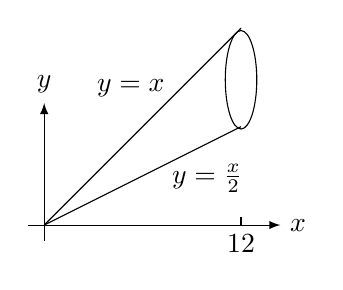
\begin{tikzpicture}
\draw[-latex](-0.2,0)--(3,0)node[right]{$x$};
\draw[-latex](0,-0.2)--++(0,1.75)node[above]{$y$};
\draw(2.5,0)node[below]{$12$}--++(0,0.1);
\draw plot[domain=0:2.5] ({\x},{\x/2});
\draw plot[domain=0:2.5] ({\x},{\x});
\draw(2.5,1.845) circle (0.2cm and 0.625cm);
\draw(1.5,{1.5/2})node[below right,yshift=1ex]{$y=\frac{x}{2}$};
\draw(1.5,1.5)node[above left,xshift=1ex]{$y=x$};
\end{tikzpicture}
\caption{عمودی تراش (سوال \حوالہ{سوال_تکمل_استعمال_ٹھوس_جسم_حجم_ب})}
\label{شکل_سوال_تکمل_استعمال_ٹھوس_جسم_حجم_ب}
\end{minipage}\hfill
\begin{minipage}{0.45\textwidth}
\centering
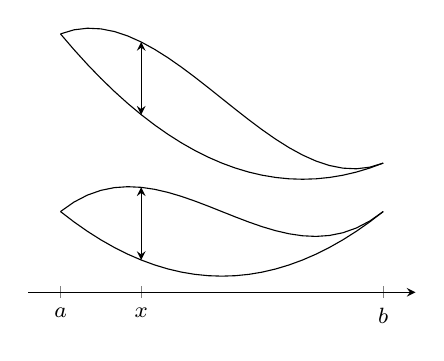
\begin{tikzpicture}[declare function={fa(\x)=1.25+\x^3-3*\x^2+2*\x;fb(\x)=1.25+\x^2-2*\x;fc(\x)=4+\x^2-3*\x;fd(\x)=fa(\x)-fb(\x)+fc(\x);}]
\begin{axis}[small,axis lines=middle,xmin=0,ymin=0,xtick={0,0.5,2},xticklabels={$a$,$x$,$b$},ytick={\empty},axis y line=none,enlargelimits=true]
\addplot[domain=0:2]{fa(x)};
\addplot[domain=0:2]{fb(x)};
\addplot[domain=0:2]{fc(x)};
\addplot[domain=0:2]{fd(x)};
\draw[stealth-stealth](axis cs:0.5,{fa(0.5)})--(axis cs:0.5,{fb(0.5)});
\draw[stealth-stealth](axis cs:0.5,{fc(0.5)})--(axis cs:0.5,{fd(0.5)});
\end{axis}
\end{tikzpicture}
\caption{وقفہ $[a,b]$ پر کسی بھی $x$ پر دونوں خطوں کی چوڑائی ایک دوسرے جتنی ہے (مسئلہ کوالئیرے)۔}
\label{شکل_سوال_تکمل_استعمال_چوڑائی_برابر}
\end{minipage}
\end{figure}
\begin{figure}
\centering
\begin{minipage}{0.45\textwidth}
\centering
\begin{tikzpicture}[font=\scriptsize]
\pgfmathsetmacro{\la}{1.25}
\pgfmathsetmacro{\laa}{\la/2}
\pgfmathsetmacro{\h}{4/3*\la}
\draw[-stealth](0,0)--++(\la,0)node[pos=0.5,fill=white]{$R$};
\draw(0,-0.1)--++(0,0.2);
\draw[stealth-stealth](-\la-0.3,0)--++(0,-\h)node[pos=0.5,left]{$R$};
\draw(0,0) circle (\la cm and 0.25*\la cm);
\draw[dashed]([shift={(0:\la cm and 0.25*\la cm)}]0,-\h) arc (0:180:\la cm and 0.25*\la cm);
\draw([shift={(180:\la cm and 0.25*\la cm)}]0,-\h) arc (180:360:\la cm and 0.25*\la cm);
\draw(-\la,0)--++(0,-\h) (\la,0)--++(0,-\h);
\draw(-\la,0)--(0,-\h)--(\la,0);
\draw(0,-\h/2) circle (\laa cm and 0.25*\laa cm);
\draw(0,-\h)--(0,-\h/2)node[pos=0.6,left]{$h$}--++(\laa,0)node[pos=0.5,above,fill=white]{$h$};
\begin{scope}[xshift=-3.5cm,yscale=1.5]
\draw([shift={(180:\la cm and 0.25*\la cm)}]0,-2/3*\h) arc (180:360:\la cm and 0.25*\la cm);
\draw[dashed]([shift={(0:\la cm and 0.25*\la cm)}]0,-2/3*\h) arc (0:180:\la cm and 0.25*\la cm);
\draw([shift={(0:\la cm)}]0,-2/3*\h) arc (0:180:\la)node[pos=0.75,left]{\RL{نصف کرہ}};
\draw(0,-2/3*\h)--++(0,\h/3)node[pos=0.35,left]{$h$}--++({sqrt(\la^2-(\h/3)^2)},0)node[pos=0.5,above,xshift=-1ex]{$\sqrt{R^2-h^2}$}--(0,-2/3*\h)node[pos=0.6,below right]{$R$};
\end{scope}
\end{tikzpicture}
\caption{کرہ اور بیلن سے مخروط منفی کر کے ایک جیسا حجم ملتا ہے (سوال \حوالہ{سوال_تکمل_استعمال_نصف_کرہ_حجم})۔}
\label{شکل_سوال_تکمل_استعمال_نصف_کرہ_حجم}
\end{minipage}
\end{figure}
\ابتدا{سوال}\شناخت{سوال_تکمل_استعمال_چوڑائی_برابر}\ترچھا{مسئلہ کوالئیرے کی ابتدائی صورت}\\
کوالئیرے نے طالب علمی کے دوران دریافت کیا کہ اگر دو مستوی خطوں کو \عددی{x} محور کے یکساں وقفہ پر یوں رکھنا ممکن ہو کہ کسی بھی \عددی{x} پر دونوں خطوں کی چوڑائی ایک دوسرے جیسی ہو تب دونوں خطوں کا رقبہ ایک دوسرے جیسا ہو گا (شکل \حوالہ{شکل_سوال_تکمل_استعمال_چوڑائی_برابر})۔ ٹھوس اجسام کے لئے یہی مسئلہ کوالئیرے نے کبھی ثابت نہیں کیا۔ اگر شکل \حوالہ{سوال_تکمل_استعمال_چوڑائی_برابر} میں بالائی اور زیریں سرحدیں استمراری تفاعل ہوں تب اس مسئلے کو ثابت کریں۔

\انتہا{سوال}
%======================
\ابتدا{سوال}\شناخت{سوال_تکمل_استعمال_نصف_کرہ_حجم}\ترچھا{نصف کرہ کا حجم بذریعہ مسئلہ کوالئیرے}\\
نصف کرہ کا حجم \عددی{H=\tfrac{2}{3}\pi R^3} ہے جہاں \عددی{R} رداس ہے۔رداس \عددی{R} اور قد \عددی{R} کے قائمہ بیلن سے  رداس \عددی{R} اور قد \عددی{R} کا قائمہ مخروط ہٹا کر نصف کرہ کا عمودی تراش حاصل ہوتا ہے۔ مخروط کو نوک کے بل رکھا تصور کریں (شکل \حوالہ{شکل_سوال_تکمل_استعمال_نصف_کرہ_حجم})۔اس حقیقت کو استعمال کرتے ہوئے نصف کرہ کا حجم تلاش کریں۔  
\انتہا{سوال}
%===========================

\حصہ{اجسام طواف کے حجم۔ قرص اور چھلا}
مستوی خطے کو کسی محور کے گرد گمانے سے \اصطلاح{جسم طواف}\فرہنگ{جسم طواف}\حاشیہب{solid of revolution}\فرہنگ{solid of revolution} پیدا کیا جاتا ہے (شکل \حوالہ{شکل_تکمل_استعمال_جسم_طواف})۔ جسم طواف پیدا کرنے کے لئے گھمائے جانے والے مستوی خطے کو \اصطلاح{پیدا کار خطہ}\فرہنگ{پیداکار خطہ}\حاشیہب{generating region}\فرہنگ{generating!region} کہتے ہیں۔ جسم طواف کا حجم ٹکیوں کی ترکیب سے نہایت خوش اسلوبی سے حاصل ہوتا ہے۔
\begin{figure}
\centering
\begin{tikzpicture}
\pgfmathsetmacro{\la}{1}
\pgfmathsetmacro{\lb}{\la/2}
\pgfmathsetmacro{\lc}{2/3*\la}
\pgfmathsetmacro{\ld}{\lc/2}
\pgfmathsetmacro{\le}{2/3*\ld}
\pgfmathsetmacro{\lf}{\le/2}
\pgfmathsetmacro{\w}{0.3}
\pgfmathsetmacro{\len}{4}
\pgfmathsetmacro{\ang}{135}
\draw(0,0)circle (\lb cm and \la cm);
\draw(0,\la)--++(-\w,0)  (0,-\la)--++(-\w,0);
\draw([shift={(90:\lb cm and \la cm)}]-\w,0) arc (90:270:\lb cm and \la cm); 
\draw[fill=white]([shift={(90:\ld cm and \lc cm)}]0,0) arc (90:270:\ld cm and \lc cm) (0,\lc)--++(\len,0)--++(0,-2*\lc)--++(-\len,0);
\draw[fill=white]([shift={(-90:\lb cm and \la cm)}]\len,0) arc (-90:90:\lb cm and \la cm)--++(-\w,0) arc (90:270:\lb cm and \la cm)--++(\w,0);
\draw[shift={(90:\lb cm and \la cm)}](\len,0) arc (90:270:\lb cm and \la cm);
\draw(\len,0) circle (\lf cm and \le cm);
\draw[dashed](-1,0)--(\len,0);
\draw(\len,0)--++(1.5,0);
\path(-\w,0)++(\ang:\lf cm and \le cm)coordinate(ka);
\path(\ang:\lb cm and \la cm)coordinate(kc)++(-\w,0)coordinate(kb);
\path(\ang:\ld cm and \lc cm)coordinate(kd);
\path(\len-\w,0)++(\ang:\ld cm and \lc cm)coordinate(ke);
\path(\len-\w,0)++(\ang:\lb cm and \la cm)coordinate(kf)++(\w,0)coordinate(kg);
\path(\len,0)++(\ang:\lf cm and \le cm)coordinate(kh);
\draw[fill=lgray,opacity=0.5](ka)--(kb)--(kc)--(kd)--(ke)coordinate[pos=0.5](kgen)--(kf)--(kg)--(kh)--cycle;
\draw(kgen)--++(45:1)node[above]{\RL{پیداکار خطہ}};
\draw[-stealth,thick,gray] ([shift={(-100:0.25cm and 0.5cm)}]\len+1,0) arc (-100:220:0.25cm and 0.5cm)node[pos=0.5,above]{\RL{محور طواف}};
\end{tikzpicture}
\caption{مستوی خطہ کو کسی محور کے گرد گھما کر جسم طواف پیدا کیا جاتا ہے۔}
\label{شکل_تکمل_استعمال_جسم_طواف}
\end{figure}
%

\begin{figure}
\centering
\begin{subfigure}{0.45\textwidth}
\centering
\begin{tikzpicture}
\pgfmathsetmacro{\angA}{20}
\pgfmathsetmacro{\angB}{170}
\pgfmathsetmacro{\len}{2}
\pgfmathsetmacro{\ra}{0.75}
\pgfmathsetmacro{\rb}{1.25}
\pgfmathsetmacro{\rc}{0.92*\rb}
\pgfmathsetmacro{\angS}{-140}
\pgfmathsetmacro{\angE}{140}
\draw(0,\ra)coordinate(uL) to [out=\angA,in=\angB] coordinate[pos=0.5](kA)(\len,\rb);
\draw(0,-\ra)coordinate(lL) to [out=-\angA,in=-\angB] coordinate[pos=0.5](kB)(\len,-\rb);
\draw([shift={(\angS:0.5*\rb cm and \rb cm)}]\len,0) arc( \angS:\angE:0.5*\rb cm and \rb cm)coordinate[pos=0](kSb)coordinate[pos=1](kEb);
\draw(kSb)--(\len,0)--(kEb);
\draw([shift={(\angS:0.5*\ra cm and \ra cm)}]0,0) arc( \angS:-90:0.5*\ra cm and \ra cm)coordinate[pos=0](kSa);
\draw([shift={(90:0.5*\ra cm and \ra cm)}]0,0) arc( 90:\angE:0.5*\ra cm and \ra cm)coordinate[pos=1](kEa);
\draw(kSa)--(0,0)--(kEa);
\draw[-latex](-1,0)--(\len+2,0)node[right]{$x$};
\draw[-latex](-0.75,-0.2)--++(0,2)node[above]{$y$};
\draw([shift={(0:0.5*\rc cm and \rc cm)}]1/2*\len,0) arc (0:360:0.5*\rc cm and \rc cm)coordinate[pos=0.2](kname);
\draw[-stealth](1/2*\len,0)--++(-155:0.5*\rc cm and \rc cm)node[pos=0.75,right,font=\footnotesize]{$R(x)$};
\draw(kname) to [out=70,in=-155]++(0.5,1)node[right,align=center]{\RL{قرص کا رقبہ عمودی تراش}\\  $S(x)=\pi (R(x))^2$};
\draw(kSa) to [out=\angA,in=\angB](kSb);
\draw[thick](kEa) to[out=-\angA,in=-\angB] coordinate[pos=0.35](kfun)(kEb);
\draw(0,0)node[above left,xshift=-0.5ex]{$a$} (\len,0)node[above right]{$b$};
\draw(kfun)--++(120:1)node[above,xshift=3ex]{$y=R(x)$};
\draw(\len+1,0)++(0,-0.1)--++(-45:0.5)node[below]{\RL{محور طواف}};
\end{tikzpicture}
\caption{استمراری تفاعل $y=R(x)$ کو $x=a$ تا $x=b$ محور $x$ کے گرد گھمایا گیا ہے۔}
\end{subfigure}\hfill
\begin{subfigure}{0.45\textwidth}
\centering
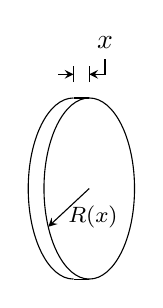
\begin{tikzpicture}
\pgfmathsetmacro{\ra}{0.75}
\pgfmathsetmacro{\rb}{1.25}
\pgfmathsetmacro{\rc}{0.92*\rb}
\draw([shift={(0:0.5*\rc cm and \rc cm)}]0,0) arc (0:360:0.5*\rc cm and \rc cm);
\draw(0,\rc)--++(-0.2,0);
\draw(0,-\rc)--++(-0.2,0);
\draw([shift={(90:0.5*\rc cm and \rc cm)}]-0.2,0) arc (90:270:0.5*\rc cm and \rc cm);
\draw[-stealth](0,0)--++(-155:0.5*\rc cm and \rc cm)node[pos=0.75,right,font=\footnotesize]{$R(x)$};
\draw(0,\rc+0.2)--++(0,0.2)coordinate[pos=0.5](kr);
\draw(-0.2,\rc+0.2)--++(0,0.2)coordinate[pos=0.5](kl);
\draw[stealth-](kl)--++(-0.2,0);
\draw[stealth-](kr)--++(0.2,0)--++(0,0.2)node[above]{$\dif x$};
\end{tikzpicture}
\caption{قرص کا حجم $\dif H=\pi (R(x))^2$ ہے۔}
\end{subfigure}
\caption{جسم طواف کے حجم کا حصول بذریعہ ترکیب قرص۔}
\label{شکل_تکمل_استعمال_استمراری_مستوی_پیداکار}
\end{figure}

اگر ہم مستوی خطہ کو استمراری تفاعل \عددی{y=R(x),\, a\le x\le b}  اور \عددی{x} کے بیچ خطہ سے ظاہر کر سکیں اور اگر \عددی{x} محور گھومنے کا محور (\اصطلاح{محور طواف}\فرہنگ{محور!طواف}\حاشیہب{axis of revolution}\فرہنگ{axis!of revolution}) بھی ہو تب ٹھوس جسم کا حجم درج ذیل طریقہ سے حاصل کیا جا سکتا ہے (شکل \حوالہ{شکل_تکمل_استعمال_استمراری_مستوی_پیداکار})۔

محور طواف کے لحاظ سے عمودی تراش کا رداس \عددی{R(x)} اور رقبہ درج ذیل ہو گا۔
\begin{align*}
S(x)=\pi (\text{رداس})^2=\pi[R(x)]^2
\end{align*} 
جسم کا حجم، \عددی{x=a} تا \عددی{x=b}، تفاعل \عددی{S} کا تکمل ہو گا۔

\موٹا{جسم طواف کا حجم (محور طواف \عددی{x} محور ہے)}\\
استمراری تفاعل \عددی{y=R(x),\, a\le x\le b} کو \عددی{x} محور کے گرد گمانے سے پیدا ٹھوس جسم کا حجم درج ذیل ہو گا۔
\begin{align}\label{مساوات_تکمل_استعمال_جسم_گردش_حجم}
H=\int_a^b\pi[\text{رداس}]^2\dif x=\int_a^b\pi[R(x)]^2\dif x
\end{align}

\ابتدا{مثال}\شناخت{مثال_تکمل_استعمال_جسم_طواف_جذر}
منحنی \عددی{y=\sqrt{x},\,0\le x\le4} کو \عددی{x} محور کے گرد گمانے سے ٹھوس جسم پیدا ہوتا ہے۔ اس جسم کا حجم تلاش کریں۔

حل:\quad
ہم منحنی ترسیم کر کے ٹھوس جسم کا خاکہ بنا کر نمائندہ رداس بناتے ہیں (شکل \حوالہ{شکل_مثال_تکمل_استعمال_جسم_طواف_جذر})۔ حجم درج ذیل ہو گا۔
\begin{align*}
H&=\int_a^b\pi[R(x)]^2\dif x&&\text{\RL{مساوات \حوالہ{مساوات_تکمل_استعمال_جسم_گردش_حجم}}}\\
&=\int_0^4\pi[\sqrt{x}]^2\dif x&&R(x)=\sqrt{x}\\
&=\pi\int_0^4x\dif x=\left.\pi\frac{x^2}{2}\right\vert_0^4=\pi\frac{(4)^2}{2}=8\pi
\end{align*}
\انتہا{مثال}
%==========================
\begin{figure}
\centering
\begin{subfigure}{0.45\textwidth}
\centering
\begin{tikzpicture}[yscale=0.75,font=\small,declare function={f(\x)=sqrt(\x);}]
\draw[gray,thick]([shift={(-100:0.1cm and 0.4cm)}]4.5,0) arc (-100:100:0.1cm and 0.4cm);
\draw[-latex](-0.25,0)--(5,0)node[right]{$x$};
\draw[gray,thick,-stealth]([shift={(100:0.1cm and 0.4cm)}]4.5,0) arc (100:170:0.1cm and 0.4cm);
\draw[-latex](0,-0.2)--(0,2)node[above]{$y$};
\draw plot[domain=0:0.5]({\x},{f(\x)});
\draw plot[domain=0.5:4]({\x},{f(\x)})--(4,0)node[below]{$4$};
\draw(3,{f(3)})node[above left]{$y=\sqrt{x}$};
\draw(1,{f(1)})node[circ]{}--(1,0)node[circ]{}node[below]{$x$};
\draw[stealth-stealth](1.3,{f(1)})--(1.3,0)node[pos=0.5,right]{$R(x)=\sqrt{x}$};
\draw(1.2,{f(1)})--++(0.2,0);
\end{tikzpicture}
\caption{}
\end{subfigure}\hfill
\begin{subfigure}{0.45\textwidth}
\centering
\begin{tikzpicture}[yscale=0.75,font=\small,declare function={f(\x)=sqrt(\x);}]
\draw(-0.25,0)--(0,0);
\draw[dashed](0,0)--(4,0);
\draw[-latex](4,0)--(5,0)node[right]{$x$};
\draw(4,-0.1)--++(0,0.2)node[above]{$4$};
\draw[-latex](0,-2)--(0,2)node[above]{$y$};
\draw[thick] plot[domain=0:0.5]({\x},{f(\x)});
\draw[thick] plot[domain=0.5:4]({\x},{f(\x)});
\draw plot[domain=0:0.5]({\x},{-f(\x)});
\draw plot[domain=0.5:4]({\x},{-f(\x)});
\draw(2,{f(2)})node[above,yshift=1ex]{$y=\sqrt{x}$};
\draw(4,0) circle (0.25cm and 2cm);
\draw[](1,0) circle (0.25cm and 1cm);
\draw(1,1)--++(-0.2,0);
\draw(1,-1)--++(-0.2,0);
\draw([shift={(90:0.25cm and 1cm)}]0.8,0) arc (90:270:0.25cm and 1cm);
\draw(1,-1.2)--++(0,-0.4)coordinate[pos=0.5](kr);
\draw(0.8,-1.2)--++(0,-0.4)coordinate[pos=0.5](kl);
\draw[stealth-](kr)--++(0.2,0);
\draw[stealth-](kl)--++(-0.2,0)--++(0,-0.4)node[below]{$\dif x$};
\draw[](1,{f(1)})node[circ]{}--(1,0)node[circ]{}node[below]{$x$}node[pos=0.5,right,xshift=1ex]{$R(x)=\sqrt{x}$};
\end{tikzpicture}
\caption{}
\end{subfigure}
\caption{مستوی خطہ اور جسم طواف (مثال \حوالہ{مثال_تکمل_استعمال_جسم_طواف_جذر})}
\label{شکل_مثال_تکمل_استعمال_جسم_طواف_جذر}
\end{figure}
\موٹا{مساوات \حوالہ{مساوات_تکمل_استعمال_جسم_گردش_حجم} سے حجم حاصل کرنے کا طریقہ}\\


\begin{enumerate}[a.]
\item
خطے کا خاکہ بنائیں اور رداس \عددی{R(x)} کی نشاندہی کریں۔
\item
یوں رقبہ عمودی تراش \عددی{\pi[R(x)]^2} ہو گا۔
\item
رقبہ عمودی تراش کا تکمل حجم ہو گا۔
\end{enumerate}

اگلے مثال میں محور طواف  \عددی{x} محور نہیں ہے، لیکن حجم حاصل کرنے کا اصول تبدیل نہیں ہوتا: تکمل کے موزوں حد استعمال کریں۔

\ابتدا{مثال}\شناخت{مثال_تکمل_استعمال_جذر_منتقل}
تفاعل \عددی{y=\sqrt{x}}، لکیر \عددی{y=1} اور لکیر \عددی{x=4} کے بیچ خطہ کو لکیر \عددی{y=1} کے گرد گما کر ٹھوس جسم پیدا کیا جاتا ہے۔ اس جسم کا حجم تلاش کریں۔

حل:\quad
ہم خطہ اور نمائندہ رداس بنا کر ٹھوس جسم کا خاکہ بناتے ہیں (شکل \حوالہ{شکل_مثال_تکمل_استعمال_جذر_منتقل})۔ جسم کا حجم درج ذیل ہو گا۔
\begin{align*}
H&=\int_1^4\pi[R(x)]^2\dif x&&\text{\RL{مساوات \حوالہ{مساوات_تکمل_استعمال_جسم_گردش_حجم}}}\\
&=\int_1^4\pi[\sqrt{x}-1]^2\dif x&&R(x)=\sqrt{x}-1\\
&=\pi\int_1^4[x-2\sqrt{x}+1]\dif x\\
&=\pi\big[\frac{x^2}{2}-2\cdot\frac{2}{3}x^{3/2}+x\big]_1^4=\frac{7\pi}{6}
\end{align*}
\انتہا{مثال}
%==================== 
\begin{figure}
\centering
\begin{subfigure}{0.45\textwidth}
\centering
\begin{tikzpicture}[yscale=0.75,font=\small,declare function={f(\x)=sqrt(\x);g(\x)=1;}]
\draw[-latex](-0.25,0)--(4.5,0)node[right]{$x$};
\draw[-latex](0,-0.2)--(0,2)node[above]{$y$};
\draw plot[domain=0:0.5]({\x},{f(\x)});
\draw plot[domain=0.5:4]({\x},{f(\x)})--(4,0)node[below]{$4$};
\draw plot[domain=0:4]({\x},{g(\x)});
\draw(3.5,{f(3.5)})node[above,xshift=1ex]{$y=\sqrt{x}$};
\draw(3.5,{g(3.5)})node[below]{$y=1$};
\draw(2.5,{f(2.5)})node[circ]{}--(2.5,{g(2.5)})node[circ]{}node[below]{$x$};
\draw[stealth-stealth](2.3,{f(2.5)})--(2.3,{g(2.5)})coordinate[pos=0.5](k);
\draw(2.2,{f(2.5)})--++(0.2,0);
\draw(k)++(-0.1,0) to [out=180,in=-45]++(-0.5,0.5)node[above,xshift=-1ex]{$R(x)=\sqrt{x}-1$};
\draw(1,0)node[below]{$1$}--++(0,0.1)  (0,1)node[left]{$1$};
\draw[gray,thick] ([shift={(-80:0.2cm and 0.4cm)}]4.5,1) arc (-80:100:0.2cm and 0.4cm);
\draw(4.2,1)--++(0.7,0);
\draw[gray,thick,-stealth] ([shift={(100:0.2cm and 0.4cm)}]4.5,1) arc (100:170:0.2cm and 0.4cm);
\end{tikzpicture}
\caption{}
\end{subfigure}\hfill
\begin{subfigure}{0.45\textwidth}
\centering
\begin{tikzpicture}[yscale=0.75,font=\small,declare function={f(\x)=sqrt(\x);}]
\pgfmathsetmacro{\kk}{f(2.5)-1}
\draw[-latex](-0.2,0)--(5,0)node[right]{$x$};
\draw  (1,0)node[below]{$1$}--++(0,0.1) (4,0)node[below]{$4$} (0,1)node[left]{$1$}--++(0.1,0);
\draw[-latex](0,-0.2)--(0,2)node[above]{$y$};
\draw[thick] plot[domain=1:4]({\x},{f(\x)});
\draw plot[domain=1:4]({\x},{2-f(\x)});
\draw(4,1) circle (0.25cm and 1cm);
\draw[dashed](1,1)--(4,1);
\draw(0.5,1)--(1,1)  (4,1)--(5,1);
\draw(2.5,0)node[below]{$x$}--++(0,0.1);
\draw[](2.5,1)node[circ]{}--(2.5,{f(2.5)})node[circ]{}coordinate[pos=0.5](k);
\draw(k) to [out=180,in=-45]++(-0.5,0.5)node[above]{$R(x)=\sqrt{x}-1$};
\draw(4,{f(4)})node[above]{$y=\sqrt{x}$};
\draw[dashed](2.5,1)circle (0.15cm and \kk cm);
\end{tikzpicture}
\caption{}
\end{subfigure}
\caption{مستوی خطہ اور جسم طواف (مثال \حوالہ{مثال_تکمل_استعمال_جذر_منتقل})}
\label{شکل_مثال_تکمل_استعمال_جذر_منتقل}
\end{figure}
منحنی \عددی{x=R(y),\, c\le y\le d} کو \عددی{y} محور کے گرد گما کر ٹھوس جسم پیدا ہوتا ہے جس کا حجم تلاش کرتے ہوئے مساوات \حوالہ{مساوات_تکمل_استعمال_جسم_گردش_حجم} میں \عددی{x} کی جگہ \عددی{y} لکھا جاتا ہے۔


\موٹا{جسم طواف کا حجم (محور طواف \عددی{y} محور ہے)}\\
استمراری تفاعل \عددی{x=R(y),\, c\le y\le d} کو \عددی{y} محور کے گرد گمانے سے پیدا ٹھوس جسم کا حجم درج ذیل ہو گا۔
\begin{align}\label{مساوات_تکمل_استعمال_جسم_گردش_حجم_ب}
H=\int_c^d\pi[\text{رداس}]^2\dif x=\int_c^d\pi[R(y)]^2\dif y
\end{align}

\ابتدا{مثال}\شناخت{مثال_تکمل_استعمال_معکوس}
منحنی \عددی{x=\tfrac{2}{y},\, 1\le y \le 4} کو \عددی{y} محور کے گرد گھما کر جسم طواف پیدا کیا جاتا ہے۔ اس جسم کا حجم دریافت کریں۔

حل:\quad
ہم منحنی ترسیم کر کے ٹھوس جسم کا خاکہ بنا کر نمائندہ قرص اور رداس بناتے ہیں (شکل \حوالہ{شکل_مثال_تکمل_استعمال_معکوس})۔ جسم کا حجم درج ذیل ہو گا۔
\begin{align*}
H&=\int_1^4\pi[R(y)]^2\dif y&&\text{\RL{مساوات \حوالہ{مساوات_تکمل_استعمال_جسم_گردش_حجم_ب}}}\\
&=\int_1^4\pi\big(\frac{2}{y}\big)^2\dif y&&R(y)=\frac{2}{y}\\
&=\pi\int_1^4\frac{4}{y^2}\dif y=4\pi\big[-\frac{1}{y}\big]_1^4=4\pi\big[\frac{3}{4}\big]=3\pi
\end{align*}
\انتہا{مثال}
%=======================
\begin{figure}
\centering
\begin{subfigure}{0.45\textwidth}
\centering
\begin{tikzpicture}[yscale=0.5,declare function={f(\x)=2/(\x);}]
\draw[]plot[domain=0.5:2]({\x},{f(\x)});
\draw({0.5},{f(0.5)})node[right,yshift=-1ex]{$x=\frac{2}{y}$};
\draw[-latex] (-0.2,0)--(2.5,0)node[right]{$x$};
\draw[gray,thick] ([shift={(-20:0.5cm and 0.2cm)}]0,5) arc (-20:135:0.5cm and 0.2cm);
\draw[-latex] (0,-0.2)--(0,6)node[above]{$y$};
\draw[gray,thick,-stealth]([shift={(135:0.5cm and 0.2cm)}]0,5) arc (135:270:0.5cm and 0.2cm);
\draw(0,{f(0.5)})node[left]{$4$}--(0.5,{f(0.5)});
\draw(0,{f(2)})node[left]{$1$}--(2,{f(2)});
\draw(2,0)node[below]{$2$}--++(0,0.2);
\draw(0,{f(4/5)})node[circ]{}node[left]{$y$}--(4/5,{f(4/5)})node[circ]{}coordinate[pos=0.5](kkk);
\draw(kkk) to [out=-45,in=180]++(1,-0.5)node[right]{$R(y)=\frac{2}{y}$};
\end{tikzpicture}
\caption{}
\end{subfigure}\hfill
\begin{subfigure}{0.45\textwidth}
\centering
\begin{tikzpicture}[yscale=0.5,declare function={f(\x)=2/(\x);}]
\pgfmathsetmacro{\a}{f(0.5)}
\pgfmathsetmacro{\b}{f(2)}
\pgfmathsetmacro{\c}{f(4/5)}
\draw[]plot[domain=0.5:2]({\x},{f(\x)});
\draw[]plot[domain=0.5:2]({-\x},{f(\x)});
\draw({0.5},{f(0.5)})node[right,yshift=-1ex]{$x=\frac{2}{y}$};
\draw(0,\a) circle (0.5cm and 0.2cm);
\draw([shift={(180:2 cm and 0.4cm)}]0,\b)arc (180:360:2 cm and 0.4cm);
\draw[-latex] (-2.5,0)--(2.5,0)node[right]{$x$};
\draw[] (0,-0.2)--(0,1-0.4) (2,0)node[below]{$2$}--++(0,0.2);
\draw[dashed] (0,1-0.4)--(0,4);
\draw[-latex] (0,4)node[above left]{$4$}--(0,6)node[above]{$y$};
\draw(0,{f(4/5)})node[circ]{}node[left]{$y$}--(4/5,{f(4/5)})node[circ]{}coordinate[pos=0.5](kkk);
\draw(kkk) to [out=-45,in=180]++(1,-0.5)node[right]{$R(x)=\frac{2}{y}$};
\draw[](0,{f(4/5)}) circle (0.8 cm and 0.4cm);
\draw(0,{f(4/5)})++(0.8,0)--++(0,-0.4);
\draw(0,{f(4/5)})++(-0.8,0)--++(0,-0.4);
\draw[]([shift={(180:0.8cm and 0.4cm)}]0,{f(4/5)-0.4}) arc (180:360:0.8 cm and 0.4cm);
\draw(0,{f(4/5)})++(-0.8-0.4,0)--++(-0.2,0)coordinate[pos=0.5](kt);
\draw(0,{f(4/5)})++(-0.8-0.4,-0.4)--++(-0.2,0)coordinate[pos=0.5](kb);
\draw[stealth-](kb)--++(0,-0.4);
\draw[stealth-](kt)--++(0,0.6)--++(-0.4,0)node[left]{$\dif y$};
\end{tikzpicture}
\caption{}
\end{subfigure}
\caption{مستوی خطہ، جسم طواف اور قرص (مثال \حوالہ{مثال_تکمل_استعمال_معکوس})}
\label{شکل_مثال_تکمل_استعمال_معکوس}
\end{figure}
\ابتدا{مثال}\شناخت{مثال_تکمل_استعمال_قطع_مکافی_جسم_طواف}
قطع مکافی \عددی{x=y^2+1}اور لکیر \عددی{x=3}کے بیچ خطہ کو لکیر \عددی{x=3} کے گرد گھما کر جسم طواف پیدا کیا جاتا ہے۔ جسم کا حجم معلوم کریں۔

حل:\quad
ہم منحنی اور لکیر کے بیچ خطے کا  خاکہ بنا کر جسم طواف کا خاکہ بناتے ہیں اور عمودی تراش کی نمائندہ رداس کی نشاندہی کرتے ہیں (شکل \حوالہ{شکل_مثال_تکمل_استعمال_قطع_مکافی_جسم_طواف})۔جسم کا حجم درج ذیل ہو گا۔
\begin{align*}
H&=\int_{-\sqrt{2}}^{\sqrt{2}}\pi[R(y)]^2\dif y&&\text{\RL{مساوات \حوالہ{مساوات_تکمل_استعمال_جسم_گردش_حجم_ب}}}\\
&=\int_{-\sqrt{2}}^{\sqrt{2}}\pi[2-y^2]^2\dif y&&R(y)=3-(y^2+1)\\
&=\pi\int_{-\sqrt{2}}^{\sqrt{2}}[4-4y^2+y^4]\dif y\\
&=\pi\big[4y-\frac{4}{3}y^3+\frac{y^5}{5}\big]_{-\sqrt{2}}^{\sqrt{2}}\\
&=\frac{64\pi \sqrt{2}}{15}
\end{align*}
\انتہا{مثال}
%==========================
\begin{figure}
\centering
\begin{subfigure}{0.45\textwidth}
\centering
\begin{tikzpicture}[font=\small,declare function={f(\x)=sqrt(\x-1);}]
\draw[-latex](-0.2,0)--(3.5,0)node[right]{$x$};
\draw[-latex](0,-2)--(0,2)node[above]{$y$};
\draw(1,0)node[below left]{$1$}  (3,0)node[below left]{$3$};
\draw(0,{sqrt(2)})node[left]{$\sqrt{2}$}--++(0.1,0)  (0,{-sqrt(2)})node[left]{$-\sqrt{2}$}--++(0.1,0)  ;
\draw[]plot[domain=1:1.5]({\x},{f(\x)});
\draw[]plot[domain=1:1.5]({\x},{-f(\x)});
\draw[]plot[domain=1.5:3]({\x},{f(\x)});
\draw[]plot[domain=1.5:3]({\x},{-f(\x)});
\draw[gray,thick]([shift={(70:0.4cm and 0.2cm)}]3,-2) arc (70:160:0.4cm and 0.2cm);
\draw(3,-2.3)--(3,2)node[right]{$x=3$};
\draw[gray,thick,-stealth]([shift={(160:0.4cm and 0.2cm)}]3,-2) arc (160:300:0.4cm and 0.2cm);
\draw(2,{-f(2)})node[left,yshift=-0.5ex]{$x=y^2+1$};
\draw(3,{f(3)})node[right]{$(3,\sqrt{2})$};
\draw(3,{-f(3)})node[right]{$(3,-\sqrt{2})$};
\draw(1.5,{f(1.5)})node[circ]{}--(3,{f(1.5)})node[circ]{}coordinate[pos=0.5](kk);
\draw(0,{f(1.5)})node[left]{$y$}--++(0.1,0);
\draw(kk)to[out=135,in=-90]++(-0.5,1)node[above]{$\begin{aligned}R(y)&=3-(y^2+1)\\ &=2-y^2  \end{aligned}$};
\end{tikzpicture}
\caption{}
\end{subfigure}\hfill
\begin{subfigure}{0.45\textwidth}
\centering
\begin{tikzpicture}[font=\small,declare function={f(\x)=sqrt(\x-1);}]
\pgfmathsetmacro{\a}{f(1.5)}
\draw[-latex](-0.2,0)--(5.5,0)node[right]{$x$};
\draw[-latex](0,-2)--(0,2)node[above]{$y$};
\draw(1,0)node[below left]{$1$}  (3,0)node[below left]{$3$}  (5,0)node[below right]{$5$};
\draw(0,{sqrt(2)})node[left]{$\sqrt{2}$}--++(0.1,0)  (0,{-sqrt(2)})node[left]{$-\sqrt{2}$}--++(0.1,0)  ;
\draw[]plot[domain=1:1.5]({\x},{f(\x)});
\draw[]plot[domain=1:1.5]({\x},{-f(\x)});
\draw[]plot[domain=1.5:3]({\x},{f(\x)});
\draw[]plot[domain=1.5:3]({\x},{-f(\x)});
\draw[]plot[domain=1:1.5]({6-\x},{f(\x)});
\draw[]plot[domain=1:1.5]({6-\x},{-f(\x)});
\draw[]plot[domain=1.5:3]({6-\x},{f(\x)});
\draw[]plot[domain=1.5:3]({6-\x},{-f(\x)});
\draw(3,-2.3)--(3,2);
\draw(2,{-f(2)})node[left,yshift=-0.5ex]{$x=y^2+1$};
\draw(1.5,{f(1.5)})node[circ]{}--(3,{f(1.5)})node[circ]{}coordinate[pos=0.5](kk);
\draw(0,{f(1.5)})node[left]{$y$}--++(0.1,0);
\draw(kk)to[out=135,in=-90]++(-0.5,1)node[above]{$R(y)=2-y^2$};
\draw[dashed]([shift={(0:1.5cm and 0.2cm)}]3,\a) arc (0:180:1.5cm and 0.2cm);
\draw[]([shift={(180:1.5cm and 0.2cm)}]3,\a) arc (180:360:1.5cm and 0.2cm);
\end{tikzpicture}
\caption{}
\end{subfigure}
\caption{مستوی خطہ اور جسم طواف (مثال \حوالہ{مثال_تکمل_استعمال_قطع_مکافی_جسم_طواف})}
\label{شکل_مثال_تکمل_استعمال_قطع_مکافی_جسم_طواف}
\end{figure}
\جزوحصہء{ترکیب چھلا}
اگر گھمائے جانے والا خطہ محور طواف کو قطع نہ کرتا ہو اور نا ہی محور طواف کو مس کرتا ہو تب جسم طواف میں سوراخ پایا جائے گا (شکل \حوالہ{شکل_تکمل_استعمال_ترکیب_چھلا})۔ایسے جسم کا بیرونی رداس \عددی{R(x)} اور اندرونی رداس \عددی{r(x)} ہو گا۔ یوں اس کا رقبہ عمودی تراش درج ذیل ہو گا۔
\begin{align*}
S(x)=\pi[R(x)]^2-\pi[r(x)]^2=\pi([R(x)]^2-[r(x)]^2)
\end{align*}

\موٹا{حجم تلاش کرنے کا کلیہ}\\
\begin{align}\label{مساوات_تکمل_استعمال_جسم_گردش_حجم_پ}
H=\int_a^b\pi([R(x)]^2-[r(x)]^2)\dif x
\end{align}

دھیان رہے کہ مساوات \حوالہ{مساوات_تکمل_استعمال_جسم_گردش_حجم_پ} میں تفاعل \عددی{\pi(R^2-r^2)} کا تکمل لیا جاتا ہے نا کہ تفاعل \عددی{\pi(R-r)^2} کا۔ اگر پورے وقفہ \عددی{[a,b]} پر  اندرونی رداس صفر ہو تب درج بالا  سے مساوات \حوالہ{مساوات_تکمل_استعمال_جسم_گردش_حجم}  حاصل ہوتی ہے۔ یوں ترکیب ٹکیا در حقیقت ترکیب چھلا کی مخصوص صورت ہے۔
\begin{figure}
\centering
\begin{subfigure}{0.45\textwidth}
\centering
\begin{tikzpicture}[xscale=2.5,font=\small,declare function={fa(\x)=1.25+\x^3-3*\x^2+2*\x;fb(\x)=1.25+\x^2-2*\x;}]
\pgfmathsetmacro{\a}{0.2}
\pgfmathsetmacro{\b}{1.5}
\pgfmathsetmacro{\c}{0.7}
\draw[gray,thick]([shift={(-60:0.1cm and 0.4cm)}]1.7,0) arc (-60:120:0.1cm and 0.4cm);
\draw[-latex](-0.2,0)--(2,0)node[right]{$x$};
\draw[gray,thick,-stealth]([shift={(120:0.1cm and 0.4cm)}]1.7,0) arc (120:270:0.1cm and 0.4cm);
\draw[-latex](0,-0.2)--(0,2)node[above]{$y$};
\foreach \x/\l in {\a/a,\b/b}{\draw(\x,0)node[below]{$\l$}--++(0,0.1);}
\draw[]plot[domain=\a:\b]({\x},{fa(\x)});
\draw[]plot[domain=\a:\b]({\x},{fb(\x)});
\draw(\a,{(fa(\a))})--(\a,{fb(\a)});
\draw(\b,{(fa(\b))})--(\b,{fb(\b)});
\draw(\b,{fa(\b)})node[right]{$y=R(x)$};
\draw(\b,{fb(\b)})node[right]{$y=r(x)$};
\draw(\c,{fa(\c)})node[circ]{}--(\c,{fb(\c)})node[circ]{}coordinate[pos=0.5](ka);
\draw(\c,0)node[below]{$x$}--++(0,0.1);
\draw(ka) to [out=45,in=180]++(0.5,1)node[right]{$R(x)-r(x)$};
\end{tikzpicture}
\caption{}
\end{subfigure}\hfill
\begin{subfigure}{0.45\textwidth}
\centering
\begin{tikzpicture}[xscale=2.5,font=\small,declare function={fa(\x)=1.25+\x^3-3*\x^2+2*\x;fb(\x)=1.25+\x^2-2*\x;}]
\pgfmathsetmacro{\a}{0.35}
\pgfmathsetmacro{\b}{1.5}
\pgfmathsetmacro{\c}{1}
\pgfmathsetmacro{\faa}{fa(\a)}
\pgfmathsetmacro{\fab}{fa(\b)}
\pgfmathsetmacro{\fba}{fb(\a)}
\pgfmathsetmacro{\fbb}{fb(\b)}
\pgfmathsetmacro{\fac}{fa(\c)}
\pgfmathsetmacro{\fbc}{fb(\c)}
\draw[-latex](-0.2,0)--(2,0)node[right]{$x$};
\draw[-latex](0,-2)--(0,2)node[above]{$y$};
\draw[]plot[domain=\a:\b]({\x},{fa(\x)});
\draw[dashed]plot[domain=\a:\b]({\x},{fb(\x)});
\draw[]plot[domain=\a:\b]({\x},{-fa(\x)});
\draw[dashed]plot[domain=\a:\b]({\x},{-fb(\x)});
\draw(\b,0) circle (0.1cm and \fab cm);
\draw(\b,0) circle (0.05cm and \fbb cm);
\draw[dashed]([shift={(-90:0.25cm and \faa cm)}]\a,0) arc (-90:90:0.25cm and \faa cm);
\draw([shift={(90:0.25cm and \faa cm)}]\a,0) arc (90:270:0.25cm and \faa cm);
\draw[dashed]([shift={(0:0.15cm and \fba cm)}]\a,0) arc (0:360:0.15cm and \fba cm);
\draw(\c,0) circle (0.15 cm and \fac cm);
\draw(\c,0) circle (0.05 cm and \fbc cm);
\draw(\c,{fa(\c)})--++(-0.1,0);
\draw(\c,{-fa(\c)})--++(-0.1,0);
\draw([shift={(90:0.15cm and \fac cm)}]\c-0.1,0) arc (90:270:0.15 cm and \fac cm);
\draw(\c,{fa(\c)+0.2})--++(0,0.2)coordinate[pos=0.5](kr);
\draw(\c-0.1,{fa(\c)+0.2})--++(0,0.2)coordinate[pos=0.5](kl);
\draw[stealth-](kl)--++(-0.1,0);
\draw[stealth-](kr)--++(0.1,0)--++(0,0.2)node[above]{$\dif x$};
\end{tikzpicture}
\caption{}
\end{subfigure}
\caption{یہاں جسم طواف قرص کی بجائے چھلا نما ہے جس میں سوراخ پایا جاتا ہے  لہٰذا تکمل $\int_a^bS(x)\dif x$ ذرہ مختلف صورت اختیار کرتا ہے۔}
\label{شکل_تکمل_استعمال_ترکیب_چھلا}
\end{figure}
\ابتدا{مثال}\شناخت{مثال_تکمل_استعمال_چھلا_عجیب}
منحنی \عددی{y=x^2+1} اور لکیر \عددی{y=-x+3} کے بیچ خطہ کو \عددی{x} محور کے گرد گھما کر جسم طواف پیدا کیا جاتا ہے۔ اس ٹھوس جسم کا حجم تلاش کریں۔

حل:\quad
\موٹا{پہلا قدم:}\quad
منحنی اور لکیر ترسیم کر کے خطے کا خاکہ بنا کر خطے پر محور طواف کے عمودی لکیر کھینچیں (شکل \حوالہ{شکل_مثال_تکمل_استعمال_چھلا_عجیب})۔\\
\موٹا{دوسرا قدم:}\quad
نقاط تقاطع سے تکمل کے حد تلاش کریں۔
\begin{align*}
x^2+1&=-x+3\\
x^2+x-2&=0\\
(x+2)(x-1)&=0\\
x=-2,\quad x&=1
\end{align*}
\موٹا{تیسرا قدم:}\quad
بیرونی اور اندرونی رداس کی نشاندہی کریں۔ 
\begin{align*}
R(x)&=-x+3&&\text{\RL{بیرونی رداس}}\\
r(x)&=x^2+1&&\text{\RL{اندرونی رداس}}
\end{align*}
\موٹا{چوتھا قدم:}\quad
تکمل سے حجم حاصل کریں۔
\begin{align*}
H&=\int_a^b\pi([R(x)]^2-[r(x)]^2)\dif x\\
&=\int_{-1}^{1}\pi([-x+3]^2-[x^2+1]^2)\dif x\\
&=\int_{-2}^1\pi(8-6x-x^2-x^4)\dif x\\
&=\pi\big[8x-3x^2-\frac{x^3}{3}-\frac{x^5}{5}\big]_{-2}^1=\frac{117\pi}{5}
\end{align*}
\انتہا{مثال}
%======================
\begin{figure}
\centering
\begin{subfigure}{0.45\textwidth}
\centering
\begin{tikzpicture}[font=\small,yscale=0.4,declare function={fa(\x)=-\x+3; fb(\x)=abs(\x^2)+1;}]
\draw[thick,gray]([shift={(-60:0.1cm and 0.6cm)}]-0.5,0) arc (-60:120:0.1cm and 0.6cm);
\draw[-latex](-2.5,0)--(2,0)node[right]{$x$};
\draw[thick,gray,-stealth]([shift={(120:0.1cm and 0.6cm)}]-0.5,0) arc (120:240:0.1cm and 0.6cm);
\draw[-latex](0,-0.2)--(0,5)node[above]{$y$};
\draw[]plot[domain=-2:1]({\x},{fa(\x)});
\draw[]plot[domain=-2:1]({\x},{fb(\x)});
\foreach \x in {-2,1}{\draw(\x,0)node[below]{$\x$}--++(0,0.2);}
\draw(0.7,{fa(0.7)})--++(0.25,0.75)node[above]{$y=-x+3$};
\draw(0.7,{fb(0.7)})node[below,xshift=2ex]{$y=x^2+1$};
\draw(-2,{fa(-2)})node[above]{$(-2,5)$};
\draw(1,{fa(1)})node[right]{$(1,2)$};
\draw(-1,{fa(-1)})node[circ]{}--(-1,{fb(-1)})node[circ]{}coordinate[pos=0.25](ka);
\draw(-1,0)node[below]{$x$}--++(0,0.2);
\draw(ka) to [out=-135,in=90]++(-1,-0.5)node[below,font=\footnotesize]{$\begin{aligned} &R(x)-r(x)=\\  &(-x+3)-(x^2+1)\end{aligned}$};
\end{tikzpicture}
\caption{}
\end{subfigure}\hfill
\begin{subfigure}{0.45\textwidth}
\centering
\begin{tikzpicture}[font=\small,yscale=0.4,declare function={fa(\x)=-\x+3; fb(\x)=abs(\x^2)+1;}]
\pgfmathsetmacro{\faa}{fa(-2)}
\pgfmathsetmacro{\fab}{fa(1)}
\pgfmathsetmacro{\fba}{fa(-2)}
\pgfmathsetmacro{\fbb}{fa(1)}
\pgfmathsetmacro{\fac}{fa(-1)}
\pgfmathsetmacro{\fbc}{fb(-1)}
\draw(-3,0)--(-2.4,0);
\draw[dashed](-2.4,0)--(0.8,0);
\draw[-latex](0.8,0)--(2,0)node[right]{$x$};
\draw[-latex](0,-0.2)--(0,5)node[above]{$y$};
\draw[]plot[domain=-2:1]({\x},{fa(\x)});
\draw[dashed]plot[domain=-2:1]({\x},{fb(\x)});
\draw[]plot[domain=-2:1]({\x},{-fa(\x)});
\draw[dashed]plot[domain=-2:1]({\x},{-fb(\x)});
\draw(1,0) circle (0.2cm and \fab cm); 
%\draw[dashed]([shift={(-90:0.3cm and \faa cm)}]-2,0) arc (-90:90:0.3cm and \faa cm); 
\draw[](-1,0) circle (0.2cm and \fac cm);
\draw[](-1,0) circle (0.1cm and \fbc cm);
\draw(-1,{fa(-1)})--++(-0.2,0);
\draw(-1,{-fa(-1)})--++(-0.2,0);
\draw([shift={(90:0.3cm and \fac cm)}]-1.2,0) arc (90:270:0.3cm and \fac cm); 
\draw(-1,{fa(-1)+0.5})--++(0,0.5)coordinate[pos=0.5](kkr);
\draw(-1.2,{fa(-1)+0.5})--++(0,0.5)coordinate[pos=0.5](kkl);
\draw[stealth-](kkr)--++(0.3,0);
\draw[stealth-](kkl)--++(-0.3,0)--++(0,0.7)node[above]{$\dif x$};
%\draw[thick](-1,{fa(-1)})node[circ]{}--(-1,{fb(-1)})node[circ]{};
\end{tikzpicture}
\caption{}
\end{subfigure}
\caption{مستوی خطہ اور چھلا نما جسم طواف (مثال \حوالہ{مثال_تکمل_استعمال_چھلا_عجیب})}
\label{شکل_مثال_تکمل_استعمال_چھلا_عجیب}
\end{figure}
%============================
\موٹا{ترکیب چھلا سے حجم کی تلاش}\\
\begin{enumerate}[a.]
\item
خطے کا خاکہ بنا کر اس پر محور طواف کے عمودی لکیری قطع کھینچیں۔ خطہ کو محور طواف کے گرد گھمانے سے یہ قطع نمائندہ عمودی تراش دے گا۔
\item
تکمل کے حد دریافت کریں۔
\item
عمودی تراش کا بیرونی اور اندرونی رداس کو لکیری قطع سے حاصل کریں۔
\item
تکمل کی ذریعہ حجم حاصل کریں۔
\end{enumerate}

اگر خطے کو \عددی{y} محور کے گرد گھما کر جسم طواف پیدا کیا جائے تب درج بالا اقدام استعمال کرتے ہوئے \عددی{x} کی بجائے \عددی{y} کے ساتھ تکمل لیں۔

\ابتدا{مثال}\شناخت{مثال_تکمل_استعمال_دو_منحنیات_کے_بیچ}
ربع اول میں قطع مکافی \عددی{y=x^2} اور لکیر  \عددی{y=2x} کے بیچ خطے کو \عددی{y}  محور کے گرد گھما کر جسم طواف پیدا کیا جاتا ہے۔ جسم کا حجم معلوم کریں۔

حل:\quad
\موٹا{پہلا قدم:}\quad
خطے کا خاکہ کھینچ کر خطہ پر محور طواف کے عمودی لکیری قطع بنائیں (شکل \حوالہ{شکل_مثال_تکمل_استعمال_دو_منحنیات_کے_بیچ})۔ یہاں محور طواف \عددی{y} محور ہے۔\\
\موٹا{دوسرا قدم:}\quad
قطع مکافی اور لکیر ایک دوسرے کو \عددی{y=0} اور \عددی{y=4} پر قطع کرتے ہیں لہٰذا تکمل کے حد \عددی{c=0} اور \عددی{d=4} ہوں گے۔\\
\موٹا{تیسرا قدم:}\quad
رقبہ عمودی تراش کا بیرونی رداس \عددی{R(y)=\sqrt{y}} اور اندرونی رداس \عددی{r(y)=\tfrac{y}{2}} ہے۔\\
\موٹا{چوتھا قدم:}\quad
تکمل سے حجم حاصل کرتے ہیں۔
\begin{align*}
H&=\int_c^d\pi([R(y)]^2-[r(y)]^2)\dif y\\
&=\int_0^4\pi\big([\sqrt{y}]^2-[\tfrac{y}{2}]^2\big)\dif y\\
&=\pi\int_0^4\big(y-\frac{y^2}{4}\big)\dif y=\pi\big[\frac{y^2}{2}-\frac{y^3}{12}\big]_0^4=\frac{8\pi}{3}
\end{align*} 
\انتہا{مثال}
%======================
\begin{figure}
\centering
\begin{subfigure}{0.45\textwidth}
\centering
\begin{tikzpicture}[font=\small,yscale=0.5,declare function={fa(\x)=sqrt(\x);fb(\x)=1/2*\x;}]
\pgfmathsetmacro{\a}{2}
\pgfmathsetmacro{\c}{1.2}
\draw[-latex](-0.25,0)--(2.5,0)node[right]{$x$};
\draw[-latex](0,-0.2)--(0,5,0)node[above]{$y$};
\draw[]plot[domain=0:4]({fa(\x)},{\x});
\draw[]plot[domain=0:4]({fb(\x)},{\x});
\draw(0,4)node[left]{$4$}--++(0.1,0)  (2,0)node[below]{$2$}--++(0,0.2) (0,\c)node[left]{$y$}--++(0.1,0);
\draw({fa(4)},4)node[above]{$(2,4)$};
\draw({fb(\c)},\c)node[circ]{}--({fa(\c)},\c)node[circ]{};
\draw({fa(3)},3)node[right]{$x=\sqrt{y}$};
\draw({fb(3.5)},3.5)--++(120:1.5)node[above]{$x=\tfrac{y}{2}$};
\draw({fa(\c)},\c)++(0,0.2)--++(0,2)coordinate[pos=0.9](kt);
\draw[stealth-stealth](kt)--++({-fa(\c)},0)node[pos=0.5,above]{$R(x)$};
\draw({fb(\c)},\c)++(0,0.2)--++(0,0.5)coordinate[pos=0.9](kt);
\draw[stealth-stealth](kt)--++({-fb(\c)},0)node[pos=0.5,above]{$r(x)$};
\end{tikzpicture}
\caption{}
\end{subfigure}\hfill
\begin{subfigure}{0.45\textwidth}
\centering
\begin{tikzpicture}[font=\small,yscale=0.5,declare function={fa(\x)=sqrt(\x);fb(\x)=1/2*\x;}]
\pgfmathsetmacro{\a}{2}
\pgfmathsetmacro{\c}{1.5}
\pgfmathsetmacro{\fac}{fa(\c)}
\pgfmathsetmacro{\fbc}{fb(\c)}
\draw[-latex](-2,0)--(2.5,0)node[right]{$x$};
\draw[-latex](0,-0.2)--(0,5,0)node[above]{$y$};
\draw[]plot[domain=0:4]({fa(\x)},{\x});
\draw[]plot[domain=0:4]({fb(\x)},{\x});
\draw[]plot[domain=0:4]({-fa(\x)},{\x});
\draw[]plot[domain=0:4]({-fb(\x)},{\x});
\draw(0,4)node[left]{$4$}--++(0.1,0)  (2,0)node[below]{$2$}--++(0,0.2) (0,\c);
\draw(0,\c) circle(\fac cm and 0.4cm);
\draw(0,\c) circle(\fbc cm and 0.2cm);
\draw({-fa(\c)},\c)--++(0,-0.3);
\draw({fa(\c)},\c)--++(0,-0.3);
\draw([shift={(180:\fac cm and 0.4cm)}]0,\c-0.3) arc (180:360:\fac cm and 0.4cm);
\draw({fb(3.5)},3.5)node[left,yshift=0.5ex]{$x=\tfrac{y}{2}$};
\draw({fa(3)},3)node[right]{$x=\sqrt{y}$};
\begin{scope}[]
\clip (0,\c) circle(\fbc cm and 0.2cm);
\draw(0,\c-0.2) circle(\fbc cm and 0.2cm);
\end{scope}
\end{tikzpicture}
\caption{}
\end{subfigure}
\caption{جسم طواف اور نمائندہ چھلا (مثال \حوالہ{مثال_تکمل_استعمال_دو_منحنیات_کے_بیچ})}
\label{شکل_مثال_تکمل_استعمال_دو_منحنیات_کے_بیچ}
\end{figure}
\ابتدا{مثال}\شناخت{مثال_تکمل_استعمال_پیچیدہ}
ربع اول میں قطع مکافی \عددی{y=x^2}، لکیر \عددی{y=1} اور \عددی{y} محور  کے بیچ خطہ کو لکیر \عددی{x=\tfrac{3}{2}} کے گرد گھما کر جسم طواف پیدا کیا جاتا ہے۔ اس ٹھوس جسم کا حجم دریافت کریں۔

حل:\quad
\موٹا{پہلا قدم:}\quad
خطے کے خاکہ پر محور طواف \عددی{x=\tfrac{3}{2}} کے عمودی، لکیری قطع بنائیں (شکل \حوالہ{شکل_مثال_تکمل_استعمال_پیچیدہ})۔\\
\موٹا{دوسرا قدم:}\quad
تکمل کے حد \عددی{y=0} اور \عددی{y=1} ہیں۔\\
\موٹا{تیسرا قدم:}\quad
عمودی تراش کا بیرونی رداس \عددی{R(y)=\tfrac{3}{2}} اور اندرونی رداس \عددی{r(y)=\tfrac{3}{2}-\sqrt{y}} ہے۔\\
\موٹا{چوتھا قدم:}\quad
تکمل سے حجم حاصل کرتے ہیں۔
\begin{align*}
H&=\int_c^d\pi([R(y)]^2-[r(y)]^2)\dif y\\
&=\int_0^1\pi([\tfrac{3}{2}]^2-[\tfrac{3}{2}-\sqrt{y}]^2)\dif y\\
&=\pi\int_0^1(3\sqrt{y}-y)\dif y=\pi\big[2y^{3/2}-\tfrac{y^2}{2}\big]_0^1=\frac{3\pi}{2}
\end{align*}
\انتہا{مثال}
%=======================
\begin{figure}
\centering
\begin{subfigure}{0.3\textwidth}
\centering
\begin{tikzpicture}[xscale=2,yscale=2,font=\small,declare function={fa(\x)=\x^2;}]
\pgfmathsetmacro{\c}{0.7}
\draw[-latex](-0.2,0)--(2,0)node[right]{$x$};
\draw[-latex](0,-0.2)--(0,1.5)node[above]{$y$};
\draw[]plot[domain=0:1]({\x},{fa(\x)});
\draw(0,1)node[left]{$1$}--(1,1);
\draw[thick,gray]([shift={(-50:0.3cm and 0.1cm)}]1.5,1) arc (-50:120:0.3cm and 0.1cm);
\draw(1,0)node[below]{$1$}--++(0,0.1)  (1.5,0)node[below]{$\tfrac{3}{2}$}--++(0,1.5)node[pos=0.9,right]{$x=\tfrac{3}{2}$};
\draw[thick,gray,-stealth]([shift={(120:0.3cm and 0.1cm)}]1.5,1) arc (120:240:0.3cm and 0.1cm);
\draw(0.5,{fa(0.5)})node[right]{$x=\sqrt{y}$};
\draw[stealth-stealth](0,1.25)--(1.5,1.25)node[pos=0.5,fill=white]{$R(x)$};
\draw(\c,{fa(\c)})node[circ]{}--(0,{fa(\c)})node[circ]{}node[pos=0.5,above,font=\footnotesize]{$R(x)-r(x)$};
\draw[stealth-stealth](\c,{fa(\c)})--(1.5,{fa(\c)})node[pos=0.5,fill=white]{$r(x)$};
\end{tikzpicture}
\caption{}
\end{subfigure}\hfill
\begin{subfigure}{0.6\textwidth}
\centering
\begin{tikzpicture}[xscale=2,yscale=2,font=\small,declare function={fa(\x)=\x^2;}]
\pgfmathsetmacro{\c}{0.7}
\pgfmathsetmacro{\R}{1.5}
\pgfmathsetmacro{\Rt}{\R-1}
\pgfmathsetmacro{\r}{1.5-sqrt(fa(\c))}
\draw[-latex](3,0)--(3.25,0)node[right]{$x$};
\draw[-latex](0,-0.2)--(0,1.5)node[above]{$y$};
\draw[dashed]plot[domain=0:1]({\x},{fa(\x)});
\draw[dashed]plot[domain=0:1]({3-\x},{fa(\x)});
\draw(1.5,1)circle (\Rt cm and 0.1cm);
\draw(1.5,1)circle (\R cm and 0.2cm);
\draw(3,1)--(3,0);
\draw([shift={(180:\R cm and 0.15 cm)}]1.5,0) arc (180:360:\R cm and 0.15cm);
\draw(1.5,1-0.1)--++(0,0.6)node[above]{$x=\tfrac{3}{2}$};
\draw(1.5,{fa(\c)}) circle (\R cm and 0.15cm);
\draw(1.5,{fa(\c)}) circle (\r cm and 0.1cm);
\draw([shift={(180:\R cm and 0.15 cm)}]1.5,{fa(\c)-0.05}) arc (180:360:\R cm and 0.15cm);
\begin{scope}
\clip(1.5,{fa(\c)}) circle (\r cm and 0.1cm);
\draw(1.5,{fa(\c)-0.05}) circle (\r cm and 0.1cm);
\end{scope}
\draw(0,{fa(\c)})++(-0.1,0)--++(-0.2,0)coordinate[pos=0.5](kt);
\draw(0,{fa(\c)-0.05})++(-0.1,0)--++(-0.2,0)coordinate[pos=0.5](kb);
\draw[stealth-] (kt)--++(0,0.2)--++(-0.2,0)node[left]{$\dif y$};
\draw[stealth-](kb)--++(0,-0.2);
\end{tikzpicture}
\caption{}
\end{subfigure}
\caption{جسم طواف اور نمائندہ چھلا (مثال \حوالہ{مثال_تکمل_استعمال_پیچیدہ})}
\label{شکل_مثال_تکمل_استعمال_پیچیدہ}
\end{figure}

\حصہء{سوالات}
\موٹا{حجم بذریعہ ترکیب ٹکیا}\\
سوال \حوالہ{سوال_تکمل_استعمال_جسم_طواف_الف} تا سوال \حوالہ{سوال_تکمل_استعمال_جسم_طواف_ب} میں سایہ دار خطے کو دیے گئے محور کے گرد گھما کر جسم طواف پیدا کیا جاتا ہے۔ اس جسم کا حجم دریافت کریں۔

\begin{figure}
\centering
\begin{minipage}{0.2\textwidth}
\centering
\begin{tikzpicture}[font=\tiny,declare function={f(\x)=1-\x/2;}]
\begin{axis}[axis on top,width=4cm,axis lines=middle,xlabel={$x$},ylabel={$y$},xlabel style={at={(current axis.right of origin)},anchor=west},ylabel style={at={(current axis.above origin)},anchor=south},xtick={2},ytick={1},enlargelimits=true]
\addplot[domain=-0.25:2.25]{f(x)}node[pos=0.5,above right]{$x+2y=2$};
\addplot[name path=fun,domain=0:2,draw=none]{f(x)};
\draw[name path=axis](axis cs:0,0)--(axis cs:2,0);
\addplot[fill=lgray]fill between[of=axis and fun];
\end{axis}
\end{tikzpicture}
\caption{}
\label{شکل_سوال_تکمل_استعمال_جسم_طواف_الف}
\end{minipage}\hfill
\begin{minipage}{0.2\textwidth}
\centering
\begin{tikzpicture}[font=\tiny,declare function={f(\x)=2/3*\x;}]
\begin{axis}[axis on top,width=4cm,axis lines=middle,xlabel={$x$},ylabel={$y$},xlabel style={at={(current axis.right of origin)},anchor=west},ylabel style={at={(current axis.above origin)},anchor=south},xtick={3},ytick={2},enlargelimits=true]
\addplot[domain=-0.25:3.25]{f(x)}node[pos=0.65,below right]{$x=\tfrac{3y}{2}$};
\draw(axis cs:0,2)--(axis cs:3,2);
\addplot[name path=fun,domain=0:3,draw=none]{f(x)};
\draw[name path=axis](axis cs:0,0)--(axis cs:0,2);
\addplot[fill=lgray]fill between[of=axis and fun];
\end{axis}
\end{tikzpicture}
\caption{}
\label{شکل_سوال_تکمل_استعمال_جسم_طواف_پ}
\end{minipage}\hfill
\begin{minipage}{0.2\textwidth}
\centering
\begin{tikzpicture}[font=\tiny,declare function={f(\x)=tan(deg(pi/4*\x));}]
\begin{axis}[axis on top,width=4cm,axis lines=middle,xlabel={$x$},ylabel={$y$},xlabel style={at={(current axis.right of origin)},anchor=west},ylabel style={at={(current axis.above origin)},anchor=south},xtick={\empty},ytick={1},enlargelimits=true]
\addplot[domain=-0.25:1.25]({f(x)},{x})node[pos=0.45,right,yshift=-0.5ex]{$x=\tan(\tfrac{\pi y}{4})$};
\draw(axis cs:0,1)--(axis cs:1,1);
\addplot[name path=fun,domain=0:1,draw=none]({f(x)},x);
\draw[name path=axis](axis cs:0,0)--(axis cs:0,1);
\addplot[fill=lgray]fill between[of=axis and fun];
\end{axis}
\end{tikzpicture}
\caption{}
\label{شکل_سوال_تکمل_استعمال_جسم_طواف_ت}
\end{minipage}\hfill
\begin{minipage}{0.2\textwidth}
\centering
\begin{tikzpicture}[font=\tiny,declare function={f(\x)=sin(deg(\x))*cos(deg(\x));}]
\pgfmathsetmacro{\k}{pi/2}
\begin{axis}[clip=false,axis on top,width=4cm,axis lines=middle,xlabel={$x$},ylabel={$y$},xlabel style={at={(current axis.right of origin)},anchor=west},ylabel style={at={(current axis.above origin)},anchor=south},xtick={3},ytick={2},enlargelimits=true]
\addplot[domain=0:pi/2]{f(x)}node[pos=0.5,above]{$y=\sin x \cos x$};
%\draw(axis cs:0,2)--(axis cs:3,2);
\addplot[name path=fun,domain=0:pi/2]{f(x)};
\draw[name path=axis](axis cs:0,0)--(axis cs:pi/2,0);
\addplot[fill=lgray]fill between[of=axis and fun];
\end{axis}
\end{tikzpicture}
\caption{}
\label{شکل_سوال_تکمل_استعمال_جسم_طواف_ب}
\end{minipage}
\end{figure}

\ابتدا{سوال}\شناخت{سوال_تکمل_استعمال_جسم_طواف_الف}
سایہ دار خطہ شکل \حوالہ{شکل_سوال_تکمل_استعمال_جسم_طواف_الف} میں دیا گیا ہے جہاں تفاعل \عددی{x+2y=2} ہے۔\\
جواب:\quad
$\tfrac{2\pi}{3}$
\انتہا{سوال}
%=========================

\ابتدا{سوال}\شناخت{سوال_تکمل_استعمال_جسم_طواف_پ}
سایہ دار خطہ شکل \حوالہ{شکل_سوال_تکمل_استعمال_جسم_طواف_پ} میں دیا گیا ہے جہاں تفاعل \عددی{x=\tfrac{3y}{2}} ہے۔
\انتہا{سوال}
%=========================

\ابتدا{سوال}\شناخت{سوال_تکمل_استعمال_جسم_طواف_ت}
سایہ دار خطہ شکل \حوالہ{شکل_سوال_تکمل_استعمال_جسم_طواف_ت} میں دیا گیا ہے جہاں تفاعل \عددی{x=\tan(\tfrac{\pi y}{4})} ہے۔\\
جواب:\quad
$4-\pi$
\انتہا{سوال}
%=========================

\ابتدا{سوال}\شناخت{سوال_تکمل_استعمال_جسم_طواف_ب}
سایہ دار خطہ شکل \حوالہ{شکل_سوال_تکمل_استعمال_جسم_طواف_ب} میں دیا گیا ہے جہاں تفاعل \عددی{y=\sin x\cos x} ہے۔
\انتہا{سوال}
%=========================
سوال \حوالہ{سوال_تکمل_استعمال_منحنیات_لکیریں_جسم_الف} تا سوال \حوالہ{سوال_تکمل_استعمال_منحنیات_لکیریں_جسم_ب} میں منحنیات اور لکیروں کے بیچ خطے کو \عددی{x} محور کے گرد گھما کر جسم طواف پیدا کیا جاتا ہے۔ جسم کا حجم تلاش کریں۔

\ابتدا{سوال}\شناخت{سوال_تکمل_استعمال_منحنیات_لکیریں_جسم_الف}
$y=x^2,\quad y=0,\quad x=2$\\
جواب:\quad
$\tfrac{32\pi}{5}$
\انتہا{سوال}
%=======================
\ابتدا{سوال}
$y=x^3,\quad y=0,\quad x=2$
\انتہا{سوال}
%=======================
\ابتدا{سوال}
$y=\sqrt{9-x^2},\quad y=0$\\
جواب:\quad
$36\pi$
\انتہا{سوال}
%=======================
\ابتدا{سوال}
$y=x-x^2,\quad y=0$
\انتہا{سوال}
%=======================
\ابتدا{سوال}
$y=\sqrt{\cos x},\quad 0\le x\le \tfrac{\pi}{2},\quad x=0,\quad y=0$\\
جواب:\quad
$\pi$
\انتہا{سوال}
%=======================
\ابتدا{سوال}\شناخت{سوال_تکمل_استعمال_منحنیات_لکیریں_جسم_ب}
$y=\sec x,\quad y=0,\quad x=-\tfrac{\pi}{4},\quad x=\tfrac{\pi}{4}$
\انتہا{سوال}
%=======================
سوال \حوالہ{سوال_تکمل_استعمال_حاصل_جسم_طواف_الف} اور سوال \حوالہ{سوال_تکمل_استعمال_حاصل_جسم_طواف_ب} میں خطے کو دیے گئے محور کے گرد گھمایا جاتا ہے۔ حاصل جسم طواف کا حجم معلوم کریں۔

\ابتدا{سوال}\شناخت{سوال_تکمل_استعمال_حاصل_جسم_طواف_الف}
ربع اول میں خطے کا بالائی سرحد لکیر \عددی{y=\sqrt{2}}، زیریں سرحد منحنی \عددی{y=\sec x\tan x} اور بایاں سرحد محور \عددی{y} ہیں۔ خطے کو لکیر \عددی{y=\sqrt{2}} کے گرد گھمایا جاتا ہے۔\\
جواب:\quad
$\pi\big(\tfrac{\pi}{2}+2\sqrt{2}-\tfrac{11}{3}\big)$
\انتہا{سوال}
%===========================
\ابتدا{سوال}\شناخت{سوال_تکمل_استعمال_حاصل_جسم_طواف_ب}
ربع اول میں خطے کا بالائی سرحد لکیر \عددی{y=2}، زیریں سرحد منحنی \عددی{y=\sec x\tan x,\, 0\le x\le \tfrac{\pi}{2}} اور بایاں سرحد محور \عددی{y} ہیں۔ خطے کو لکیر \عددی{y=2} کے گرد گھمایا جاتا ہے۔
\انتہا{سوال}
%=========================
سوال \حوالہ{سوال_تکمل_استعمال_محور_وائے_کے_گرد_الف} تا سوال \حوالہ{سوال_تکمل_استعمال_محور_وائے_کے_گرد_ب} میں منحنیات اور لکیروں کے بیچ خطے کو \عددی{y} محور کے گرد گھمایا جاتا ہے۔ جسم طواف کا حجم دریافت کریں۔

\ابتدا{سوال}\شناخت{سوال_تکمل_استعمال_محور_وائے_کے_گرد_الف}
$x=\sqrt{5}y^2,\quad x=0,\quad y=-1,\quad y=1$\\
جواب:\quad
$2\pi$
\انتہا{سوال}
%=====================
\ابتدا{سوال}
$x=y^{3/2},\quad x=0,\quad y=2$
\انتہا{سوال}
%=====================
\ابتدا{سوال}
$x=\sqrt{2\sin 2y},\quad 0\le y\le \tfrac{\pi}{2},\quad x=0$\\
جواب:\quad
$2\pi$
\انتہا{سوال}
%=====================
\ابتدا{سوال}
$x=\sqrt{\cos\tfrac{\pi y}{4}},\quad -2\le y\le 0,\quad x=0$
\انتہا{سوال}
%=====================
\ابتدا{سوال}
$x=\tfrac{2}{y+1},\quad x=0,\quad y=0,\quad y=3$\\
جواب:\quad
$3\pi$
\انتہا{سوال}
%=====================
\ابتدا{سوال}\شناخت{سوال_تکمل_استعمال_محور_وائے_کے_گرد_ب}
$x=\tfrac{\sqrt{2y}}{y^2+1},\quad x=0,\quad y=1$
\انتہا{سوال}
%=====================
\موٹا{حجم بذریعہ ترکیب چھلا}\\
سوال \حوالہ{سوال_تکمل_استعمال_حجم_سوراخ_الف} اور سوال \حوالہ{سوال_تکمل_استعمال_حجم_سوراخ_الف} میں سایہ دار خطے کو دیے گئے محور کے گرد گھمایا جاتا ہے۔جسم طواف کا حجم تلاش کریں۔

\ابتدا{سوال}\شناخت{سوال_تکمل_استعمال_حجم_سوراخ_الف}
خطہ شکل \حوالہ{شکل_سوال_تکمل_استعمال_حجم_سوراخ_الف} میں دکھایا گیا ہے۔\\
جواب:\quad
$\pi^2-2\pi$
\انتہا{سوال}
%=====================
\ابتدا{سوال}\شناخت{سوال_تکمل_استعمال_حجم_سوراخ_ب}
خطہ شکل \حوالہ{شکل_سوال_تکمل_استعمال_حجم_سوراخ_ب} میں دکھایا گیا ہے۔
\انتہا{سوال}
%=====================
\begin{figure}
\centering
\begin{minipage}{0.2\textwidth}
\centering
\begin{tikzpicture}[font=\tiny,declare function={f(\x)=sqrt(cos(deg(\x)));}]
\pgfmathsetmacro{\k}{pi/2}
\begin{axis}[clip=false,width=4cm,axis lines=middle,xlabel={$x$},ylabel={$y$},xlabel style={at={(current axis.right of origin)},anchor=west},ylabel style={at={(current axis.above origin)},anchor=south},enlargelimits=true,xtick={-\k,\k},xticklabels={$-\tfrac{\pi}{2}$,$\tfrac{\pi}{2}$},ytick={\empty}]
\addplot[domain=-pi/2:-pi/2+0.5]{f(x)};
\addplot[domain=pi/2-0.5:pi/2]{f(x)};
\addplot[domain=-pi/2+0.5:pi/2-0.5]{f(x)};
\addplot[name path=funb,domain=-pi/2:pi/2,draw=none]{f(x)}node[pos=0.85,sloped,below]{$y=\sqrt{\cos x}$};
\draw[name path=funa](axis cs:-pi/2,1)--(axis cs:pi/2,1)node[pos=0.75,above]{$y=1$};
\addplot[fill=lgray]fill between[of=funa and funb];
\draw(axis cs:-\k,0)--(axis cs:-\k,1)  (axis cs:\k,0)--(axis cs:\k,1);
\end{axis}
\end{tikzpicture}
\caption{}
\label{شکل_سوال_تکمل_استعمال_حجم_سوراخ_الف}
\end{minipage}\hfill
\begin{minipage}{0.2\textwidth}
\centering
\begin{tikzpicture}[font=\tiny,declare function={f(\x)=tan(deg(\x));}]
\pgfmathsetmacro{\k}{pi/4}
\begin{axis}[clip=false,width=4cm,axis lines=middle,xlabel={$x$},ylabel={$y$},xlabel style={at={(current axis.right of origin)},anchor=west},ylabel style={at={(current axis.above origin)},anchor=south},enlargelimits=true,xtick={1},ytick={\k},yticklabels={$\tfrac{\pi}{4}$}]
\addplot[name path=funa,domain=0:\k]({f(x)},x)node[pos=0.75,left]{$x=\tan y$};
\draw[name path=funb](axis cs:0,0)--(axis cs:1,0);
\addplot[fill=lgray]fill between[of=funa and funb];
\draw(axis cs:1,0)--(axis cs:1,\k);
\end{axis}
\end{tikzpicture}
\caption{}
\label{شکل_سوال_تکمل_استعمال_حجم_سوراخ_ب}
\end{minipage}
\end{figure}

سوال \حوالہ{سوال_تکمل_استعمال_ایکس_محور_الف} تا سوال \حوالہ{سوال_تکمل_استعمال_ایکس_محور_ب} میں دیے منحنیات اور لکیروں کے بیچ خطے کو \عددی{x} محور گھما کر جسم طواف پیدا کیا جاتا ہے۔جسم کا حجم تلاش کریں۔

\ابتدا{سوال}\شناخت{سوال_تکمل_استعمال_ایکس_محور_الف}
$y=x,\quad y=1,\quad x=0$\\
جواب:\quad
$\tfrac{2\pi}{3}$
\انتہا{سوال}
%=======================
\ابتدا{سوال}
$y=2x,\quad y=x,\quad x=1$
\انتہا{سوال}
%=======================
\ابتدا{سوال}
$y=2\sqrt{x},\quad y=2,\quad x=0$\\
جواب:\quad
$2\pi$
\انتہا{سوال}
%=======================
\ابتدا{سوال}
$y=-\sqrt{x},\quad y=-2,\quad x=0$
\انتہا{سوال}
%=======================
\ابتدا{سوال}
$y=x^2+1,\quad y=x+3$\\
جواب:\quad
$\tfrac{117\pi}{5}$
\انتہا{سوال}
%=======================
\ابتدا{سوال}
$y=4-x^2,\quad y=2-x$
\انتہا{سوال}
%=======================
\ابتدا{سوال}
$y=\sec x,\quad y=\sqrt{2},\quad -\tfrac{\pi}{4}\le x \le \tfrac{\pi}{4}$\\
جواب:\quad
$\pi(\pi-2)$
\انتہا{سوال}
%=======================
\ابتدا{سوال}\شناخت{سوال_تکمل_استعمال_ایکس_محور_ب}
$y=\sec x,\quad y=\tan x,\quad x=0,\quad x=1$
\انتہا{سوال}
%=======================

سوال \حوالہ{سوال_تکمل_استعمال_وائے_محور_معلوم_حجم_الف} تا سوال \حوالہ{سوال_تکمل_استعمال_وائے_محور_معلوم_حجم_ب} میں خطے کو \عددی{y} محور کے گرد گھمایا جاتا ہے۔ جسم طواف کا حجم معلوم کریں۔

\ابتدا{سوال}\شناخت{سوال_تکمل_استعمال_وائے_محور_معلوم_حجم_الف}
مثلث میں محیط خطہ جہاں مثلث کی  راسیں \عددی{(1,0)}، \عددی{(2,1)} اور \عددی{(1,1)} ہیں۔ \\
جواب:\quad
$\tfrac{4\pi}{3}$
\انتہا{سوال}
%=======================
\ابتدا{سوال}
مثلث جس کی  راسیں \عددی{(0,1)}، \عددی{(1,0)} اور \عددی{(1,1)} ہیں میں محیط خطہ۔ 
\انتہا{سوال}
%========================
\ابتدا{سوال}
ربع اول میں خطہ جس کی بالائی سرحد قطع مکافی \عددی{y=x^2}، زیریں سرحد محور \عددی{x} اور دایاں سرحد لکیر \عددی{x=2} ہے۔\\
جواب:\quad
$8\pi$
\انتہا{سوال}
%========================
\ابتدا{سوال}
خطہ کی بالائی سرحد منحنی \عددی{y=\sqrt{x}} اور زیریں سرحد لکیر \عددی{y=x} ہے۔ 
\انتہا{سوال}
%========================
\ابتدا{سوال}
ربع اول میں خطہ جس کا بایاں سرحد دائرہ \عددی{x^2+y^2=3}، دایاں سرحد لکیر \عددی{x=\sqrt{3}} اور بالائی سرحد لکیر \عددی{y=\sqrt{3}} ہے۔\\
جواب:\quad
$\sqrt{3}\pi$
\انتہا{سوال}
%========================
\ابتدا{سوال}\شناخت{سوال_تکمل_استعمال_وائے_محور_معلوم_حجم_ب}
خطے کی بائیں سرحد لکیر \عددی{x=4}اور دائیں سرحد دائرہ \عددی{x^2+y^2=25} ہے۔
\انتہا{سوال}
%========================
سوال \حوالہ{سوال_تکمل_استعمال_دیا_محور_الف} اور سوال \حوالہ{سوال_تکمل_استعمال_دیا_محور_ب} میں خطے کو دئے گئے محور کے گرد گھما کر جسم طواف پیدا کیا جاتا ہے۔جسم کا حجم معلوم کریں۔

\ابتدا{سوال}\شناخت{سوال_تکمل_استعمال_دیا_محور_الف}
ربع اول میں خطہ جس کی بالائی سرحد منحنی \عددی{y=x^2}، زیریں سرحد محور \عددی{x} اور دایاں سرحد لکیر \عددی{x=1} ہیں۔خطے کو لکیر \عددی{x=-1} کے گرد گھمایا جاتا ہے۔\\
جواب:\quad
$\tfrac{7\pi}{6}$
\انتہا{سوال}
%=====================
\ابتدا{سوال}\شناخت{سوال_تکمل_استعمال_دیا_محور_ب}
ربع دوم میں خطہ جس کی بالائی سرحد منحنی \عددی{y=-x^3}، زیریں سرحد محور \عددی{x} اور بایاں سرحد لکیر \عددی{x=-1} ہے۔ خطے کو لکیر \عددی{x=-2} کے گرد گھمایا جاتا ہے۔
\انتہا{سوال}
%======================
\موٹا{جسم طواف کے حجم}\\
\ابتدا{سوال}
ایک خطہ جس کی سرحدیں \عددی{y=\sqrt{x}}، \عددی{y=2} اور \عددی{x=0} ہیں کو درج ذیل کے گرد گھمایا جاتا ہے۔ ٹھوس جسم طواف کا حجم معلوم کریں۔
\begin{enumerate}[a.]
\item
محور \عددی{x}؛
\item
محور \عددی{y}؛
\item
لکیر \عددی{y=2}؛
\item
لکیر \عددی{x=4}
\end{enumerate}
جواب:\quad
(ا) \عددی{8\pi}، (ب) \عددی{\tfrac{32\pi}{5}}، (ج) \عددی{\tfrac{8\pi}{3}}، (د) \عددی{\tfrac{224\pi}{15}}
\انتہا{سوال}
%=====================
\ابتدا{سوال}
ایک تکونی خطی جس کی سرحدیں \عددی{y=2x}، \عددی{y=0} اور \عددی{x=1} ہیں کو درج ذیل کے گرد گھمایا جاتا ہے۔
\begin{enumerate}[a.]
\item
لکیر \عددی{x=1}؛
\item
لکیر \عددی{x=2}
\end{enumerate}
\انتہا{سوال}
%========================
\ابتدا{سوال}
ایک خطہ جس کی سرحدیں قطع مکافی \عددی{y=x^2} اور \عددی{y=1} ہیں کو درج ذیل کے گرد گھمایا جاتا ہے۔
\begin{enumerate}[a.]
\item
لکیر \عددی{y=1}؛
\item
لکیر \عددی{y=2}؛
\item
لکیر \عددی{y=-1}
\end{enumerate}
جواب:\quad
(ا) \عددی{\tfrac{16\pi}{15}}، (ب) \عددی{\tfrac{56\pi}{15}}، (ج) \عددی{\tfrac{64\pi}{15}}
\انتہا{سوال}
%========================
\ابتدا{سوال}
ایک مثلث جس کی راسیں \عددی{(0,0)}، \عددی{(b,0)} اور \عددی{(0,h)} ہیں میں محیط خطے کو درج ذیل کے گرد گھمایا جاتا ہے۔ جسم طواف کا حجم تکمل کی مدد سے حاصل کریں۔
\begin{enumerate}[a.]
\item
محور \عددی{x}؛
\item
محور \عددی{y}
\end{enumerate}
\انتہا{سوال}
%========================
\ابتدا{سوال}\شناخت{سوال_تکمل_استعمال_کروی_برتن}
ایک برتن کو رداس \عددی{\SI{16}{\centi\meter}} کے کرہ کا حصہ تصور کیا جا سکتا ہے۔برتن کی گہرائی \عددی{\SI{9}{\centi\meter}} ہے۔  برتن کا حجم تکمل کی مدد سے دریافت کریں (شکل \حوالہ{شکل_سوال_تکمل_استعمال_کروی_برتن})۔\\
جواب:\quad
$H=1053\pi\,\si{\centi\meter\cubed}$
\انتہا{سوال}
%=======================
\begin{figure}
\centering
\begin{minipage}{0.45\textwidth}
\begin{tikzpicture}[font=\small]
\centering
\pgfmathsetmacro{\rr}{1.5}
\pgfmathsetmacro{\h}{2*\rr/3}
\pgfmathsetmacro{\r}{sqrt(2*\rr*\h-\h^2)}
\pgfmathsetmacro{\ang}{90-asin(\r/\rr)}
\draw[-latex](-\rr-0.2,0)--(\rr+0.25,0)node[right]{$x\,(\si{\centi\meter})$};
\draw(0,-\rr)--(0,-\rr-0.4);
\draw[-latex](0,-\rr+\h-0.2)--(0,\rr+0.25)node[above]{$y\,(\si{\centi\meter})$};
\draw[dashed]([shift={(-\ang:\rr)}]0,0) arc (-\ang:180+\ang:\rr);
\draw(0,-\rr+\h) circle (\r cm and 0.2 cm);
\draw([shift={(180+\ang:\rr)}]0,0) arc (180+\ang:360-\ang:\rr);
\draw(45:\rr)node[above right]{$x^2+y^2=16^2$};
\draw[stealth-stealth](\r+0.4,-\rr+\h)--++(0,-\h)node[pos=0.5,right]{$\SI{9}{\centi\meter}$};
\draw(\r+0.3,-\rr+\h)--++(0.2,0);
\draw(\r+0.3,-\rr)--++(0.2,0);
\end{tikzpicture}
\caption{کروی برتن (سوال \حوالہ{سوال_تکمل_استعمال_کروی_برتن})}
\label{شکل_سوال_تکمل_استعمال_کروی_برتن}
\end{minipage}\hfill
\begin{minipage}{0.45\textwidth}
\centering
\begin{tikzpicture}[xscale=0.6,font=\small,declare function={f(\x)=\x/12*sqrt(36-\x^2);}]
\draw(-0.5,0)--(0,0);
\draw[-latex](6,0)--(7,0)node[right]{$x\,(\si{\centi\meter})$};
\draw[-latex](0,-1.5)--(0,2)node[above]{$y\,(\si{\centi\meter})$};
\draw[]plot[domain=0:5.5]({\x},{f(\x)});
\draw[]plot[domain=5.5:6]({\x},{f(\x)});
\draw[]plot[domain=0:5.5]({\x},{-f(\x)});
\draw[]plot[domain=5.5:6]({\x},{-f(\x)});
\draw(6,0)node[below right]{$6$};
\draw(4,{f(4)})node[above]{$y=\tfrac{x}{12}\sqrt{36-x^2}$};
\end{tikzpicture}
\caption{ناشپاتی نما گولہ (سوال \حوالہ{سوال_تکمل_استعمال_ناشپاتی})}
\label{شکل_سوال_تکمل_استعمال_ناشپاتی}
\end{minipage}
\end{figure}
\ابتدا{سوال}\شناخت{سوال_تکمل_استعمال_ناشپاتی}
منحنی \عددی{y=\tfrac{x}{12}\sqrt{36-x^2},\, 0\le x\le \SI{6}{\centi\meter}} کو \عددی{x} محور کے گرد گھما کر ناشپاتی نما پیتل کا  گولہ بنایا جاتا ہے (شکل \حوالہ{شکل_سوال_تکمل_استعمال_ناشپاتی})۔ پیتل کی کثافت \عددی{\SI{8.5}{\gram\per\centi\meter\cubed}} لیں۔ گولے کی کمیت کتنی ہو گی؟
\انتہا{سوال}
%==========================
\ابتدا{سوال}
منحنی \عددی{y=\sin x,\, 0\le x\le \pi x} کو لکیر \عددی{y=c} کے گرد گھما کر جسم طواف پیدا کیا جاتا ہے جہاں \عددی{0\le c\le 1} ہے۔
\begin{enumerate}[a.]
\item
ٹھوس جسم کی کم سے کم حجم \عددی{c} کی کتنی قیمت پر حاصل ہو گی؟ اس کم سے کم حجم کو تلاش کریں۔
\item
وقفہ \عددی{[0,1]} میں \عددی{c}کی کونسی قیمت زیادہ سے زیادہ حجم دے گی؟
\item
ٹھوس جسم کا حجم بالمقابل \عددی{c} کو پہلے \عددی{0\le c\le 1} کے لئے اور بعد میں بڑی قیمتوں کے لئے ترسیم کریں۔ جیسے جیسے  \عددی{c} کی قیمت وقفہ \عددی{[0,1]} سے دور ہوتی جاتی ہے، جسم کے حجم کو کیا ہوتا ہے؟ کیا اس کا طبعی مطلب بنتا ہے؟ اپنے جواب کی وجہ پیش کریں۔
\end{enumerate}
جواب:\quad
(ا) \عددی{c=\tfrac{2}{\pi}}، (ب) \عددی{c=0}
\انتہا{سوال}
%===========================
\ابتدا{سوال}
ہیلی کاپٹر کی پہنچ  بڑھانے کی خاطر اس کے نیچے تیل کی اضافی ٹینکی نسب کرنا مطلوب ہے۔ منحنی \عددی{y=\tfrac{1}{3}-\tfrac{x^2}{3},\, -1\le x\le 1} کو \عددی{x} محور کے گرد گھما کر ٹینکی بنائی جاتی ہے۔ اس ٹینکی میں کتنے لٹر تیل آئے گا؟
\انتہا{سوال}
%=============================
\ابتدا{سوال}\ترچھا{اندرسہ کا حجم}\\
دائری قرص \عددی{x^2+y^2\le a^2} کو لکیر \عددی{y=b\, (b>a)} کے گرد گھما کر \اصطلاح{اندرسہ}\فرہنگ{اندرسہ}\حاشیہب{torus}\فرہنگ{torus} پیدا کیا جاتا ہے۔ اس کا حجم تلاش کریں۔ (اشارہ۔ \عددی{\int_{-a}^a\sqrt{a^2-y^2}\dif y=\tfrac{\pi a^2}{2}} ہو گا چونکہ یہ رداس \عددی{a} کے نصف دائرے کا رقبہ ہے۔)\\
جواب:\quad
$H=2a^2b\pi^2$
\انتہا{سوال}
%==========================
\ابتدا{سوال}
(ا) نصف کروی برتن جس کا رداس \عددی{a} ہے میں پانی کی گہرائی \عددی{h} ہے۔ پانی کی مقدار معلوم کریں۔ (ب) نصف کروی ٹینکی جس کا رداس \عددی{\SI{5}{\meter}} ہے میں پانی داخل ہونے کی شرح \عددی{\SI{0.2}{\meter\cubed\per\second}} ہے۔ جس لمحہ پانی کی گہرائی \عددی{\SI{4}{\meter}} ہو، اس لمحہ گہرائی بڑھنے کی شرح کیا ہو گی؟
\انتہا{سوال}
%===========================
\ابتدا{سوال}
اس حصہ میں حجم کے تمام تعریف جیومیٹریائی تعریف کے عین مطابق ہیں۔
\begin{enumerate}[a.]
\item
نصف دائرہ \عددی{y=\sqrt{a^2-x^2}} کو \عددی{x} محور کے گرد گھما کر کرہ حاصل ہوتا ہے۔ قرص کے حجم کا کلیہ مساوات \حوالہ{مساوات_تکمل_استعمال_جسم_گردش_حجم} استعمال کرتے ہوئے کرہ کے حجم کا کلیہ \عددی{H=\tfrac{4}{3}\pi a^3} حاصل کریں۔
\item
رداس \عددی{r} اور قد \عددی{h} کا قائمہ مخروط کا حجم احصاء کی مدد سے حاصل کریں۔
\end{enumerate}
جواب:\quad
(ب) \عددی{H=\tfrac{\pi r^2h}{3}}
\انتہا{سوال}
%==========================

\حصہ{نلکی چھلے}
اجسام طواف کا حجم تلاش کرتے ہوئے بعض اوقات چھلا کی بجائے نلکی خول استعمال کرنا زیادہ بہتر ثابت ہوتا ہے (شکل \حوالہ{شکل_تکمل_استعمال_جسم_طواف_نلکی_الف})۔
\begin{figure}
\centering
\begin{subfigure}{0.45\textwidth}
\centering
\begin{tikzpicture}[x={(-10:1)}]
\pgfmathsetmacro{\h}{0.5}
\pgfmathsetmacro{\hh}{0}
\pgfmathsetmacro{\ra}{1.5}
\pgfmathsetmacro{\dr}{0.25}
\draw[-latex](-0.2,0)--(2,0)node[right]{$x$};
\draw[-latex](0,0)--(0,2.5)node[above]{$y$};
\draw[thick,gray,-stealth] ([shift={(-40:0.4cm and 0.2cm)}]0,2.4) arc (-40:260:0.4cm and 0.2cm);
\draw(\ra,0)--++(0,\h)--++(-\dr,0)--++(0,\h)--++(-\dr,0)--++(0,\h)--++(-\dr,0)--++(0,\h)--++(-\ra+3*\dr,0);
\end{tikzpicture}
\caption{}
\end{subfigure}\hfill
\begin{subfigure}{0.45\textwidth}
\centering
\begin{tikzpicture}[font=\small]
\pgfmathsetmacro{\h}{0.5}
\pgfmathsetmacro{\hh}{0}
\pgfmathsetmacro{\ra}{1.5}
\draw[fill=white]([shift={(0:\ra cm and 1/4*\ra cm)}]0,\hh) arc (0:180:\ra cm and 1/4*\ra cm)--++(0,-\h) arc (180:360:\ra cm and 1/4*\ra cm)--++(0,\h);
\draw([shift={(180:\ra cm and 1/4*\ra cm)}]0,\hh) arc (180:360:\ra cm and 1/4*\ra cm);
\pgfmathsetmacro{\hh}{\h}
\pgfmathsetmacro{\ra}{1.25}
\draw[fill=white]([shift={(0:\ra cm and 1/4*\ra cm)}]0,\hh) arc (0:180:\ra cm and 1/4*\ra cm)--++(0,-\h) arc (180:360:\ra cm and 1/4*\ra cm)--++(0,\h);
\draw([shift={(180:\ra cm and 1/4*\ra cm)}]0,\hh) arc (180:360:\ra cm and 1/4*\ra cm);
\pgfmathsetmacro{\hh}{2*\h}
\pgfmathsetmacro{\ra}{1}
\draw[fill=white]([shift={(0:\ra cm and 1/4*\ra cm)}]0,\hh) arc (0:180:\ra cm and 1/4*\ra cm)--++(0,-\h) arc (180:360:\ra cm and 1/4*\ra cm)--++(0,\h);
\draw([shift={(180:\ra cm and 1/4*\ra cm)}]0,\hh) arc (180:360:\ra cm and 1/4*\ra cm);
\pgfmathsetmacro{\hh}{3*\h}
\pgfmathsetmacro{\ra}{0.75}
\draw[fill=white]([shift={(0:\ra cm and 1/4*\ra cm)}]0,\hh) arc (0:180:\ra cm and 1/4*\ra cm)--++(0,-\h) arc (180:360:\ra cm and 1/4*\ra cm)--++(0,\h);
\draw([shift={(180:\ra cm and 1/4*\ra cm)}]0,\hh) arc (180:360:\ra cm and 1/4*\ra cm);
\draw[-latex](0,\hh)--(0,\hh+\h)node[left]{$y$};
\end{tikzpicture}
\caption{}
\end{subfigure}
\caption{نلکی جسم طواف}
\label{شکل_تکمل_استعمال_جسم_طواف_نلکی_الف}
\end{figure}
\جزوحصہء{نلکی کلیہ}
فرض کریں ہم \عددی{x} محور اور   وقفہ \عددی{[a,b]} پر تفاعل \عددی{y=f(x)} کے بیچ خطے  کو \عددی{y} محور کے گرد گھما کر جسم طواف حاصل کرتے ہیں۔ہمیں جسم طواف کا حجم درکار ہے۔  ہم وقفہ \عددی{[a,b]} کی خانہ بندی \عددی{P} پر منحصر مستطیلوں کو خطے کا تخمینی رقبہ لے سکتے ہیں۔ ایک نمائندہ مستطیل کی چوڑائی \عددی{\Delta x_k} اور قد \عددی{f(c_k)} ہو گا، جہاں نمائندہ مستطیل کے قاعدے کا وسط \عددی{c_k} ہے (شکل \حوالہ{شکل_تکمل_استعمال_کے_ویں_مستطیل_کا_خول})۔ہم جیومیٹری سے جانتے ہیں کہ ایسے مستطیل کو \عددی{y} محور کے گرد گھمانے سے حاصل جسم طواف کا حجم
\begin{align*}
\Delta H_k=2\pi\times \text{\RL{خول کا اوسط رداس}}\times \text{\RL{خول کا قد}}\times \text{\RL{موٹائی}}
\end{align*}  
ہو گا جو موجودہ صورت میں درج ذیل ہو گا۔
\begin{align*}
\Delta H_k=2\pi c_k f(c_k)\Delta x_k
\end{align*}
ہم \عددی{P} پر منحصر \عددی{n} مستطیلوں کو \عددی{y} محور کے گرد گھمانے سے حاصل حجم کے مجموعہ کو تخمیناً جسم طواف کا حجم لیتے ہیں۔
\begin{align*} 
H\approx \sum_{k=1}^n\Delta H_k=\sum_{k=1}^n2\pi c_kf(c_k)\Delta x_k\quad\quad \text{\RL{ریمان مجموعہ}}
\end{align*}
\عددی{\norm{P}\to 0} کرتے ہوئے اس مجموعہ کا حد ٹھوس جسم کا حجم  ہو گا:
\begin{align*}
H=\lim_{\norm{P}\to 0}\sum_{k=1}^n2\pi c_kf(c_k)\Delta x_k=\int_a^b2\pi xf(x)\dif x
\end{align*}
%
\begin{figure}
\centering
\begin{tikzpicture}[font=\small,declare function={f(\x)=2-sqrt(\x);}]
\pgfmathsetmacro{\c}{1.5}
\pgfmathsetmacro{\w}{0.2}
\pgfmathsetmacro{\ra}{\c-\w}
\pgfmathsetmacro{\rb}{\c+\w}
\pgfmathsetmacro{\angS}{0}
\pgfmathsetmacro{\angE}{240}
\pgfmathsetmacro{\d}{0.5}
\draw[-latex](0,0)--++(2.5,0)node[right]{$x$};
\draw[-latex](0,0)--++(0,2.5)node[above]{$y$};
\draw[thick,gray,-stealth]([shift={(-20:0.4cm and 0.2cm)}]0,2) arc (-20:240:0.4cm and 0.2cm);
\draw[thick]plot[domain=0.2:2]({\x},{f(\x)});
\draw[thick](0.2,0)--++(0,{f(0.2)})  (2,0)--++(0,{f(2)});
\draw(\d,{f(\d)})--++(45:0.5)node[right]{$y=f(x)$};
\draw([shift={(\angS:\ra cm and 1/4*\ra cm)}]0,{f(\c)}) arc (\angS:\angE:\ra cm and 1/4*\ra cm);
\draw([shift={(\angS:\rb cm and 1/4*\rb cm)}]0,{f(\c)}) arc (\angS:\angE:\rb cm and 1/4*\rb cm);
\draw([shift={(\angS:\ra cm and 1/4*\ra cm)}]0,0) arc (\angS:\angE:\ra cm and 1/4*\ra cm);
\draw(\ra,{f(\c)})coordinate(sI)--(\rb,{f(\c)})coordinate(sO);
\draw(sI)--++(0,-{f(\c)})  (sO)--++(0,{-f(\c)});
\path(0,{f(\c)})++(\angE:\ra cm and 1/4*\ra cm)coordinate(eI)++(0,{-f(\c)})coordinate(eIL);
\path(0,{f(\c)})++(\angE:\rb cm and 1/4*\rb cm)coordinate(eO)++(0,{-f(\c)})coordinate(eOL);
\fill[white](eO)--(eOL)--++(-1/2*\ra,0)--++(0,{f(\c)})--cycle;
\draw[fill=white](eI)--(eO)--(eOL)--(eIL)--(eI);
\draw([shift={(180:\rb cm and 1/4*\rb cm)}]0,0) arc (180:\angE:\rb cm and 1/4*\rb cm);
\draw(-\rb,0)--++(0,{f(\c)});
\draw(\c,0)node[below]{$c_k$}--++(0,0.1);
\draw(\c-\w,-0.4)--++(0,-0.3)coordinate[pos=0.5](kL);
\draw(\c+\w,-0.4)--++(0,-0.3)coordinate[pos=0.5](kR);
\draw[stealth-](kL)--++(-0.2,0);
\draw[stealth-](kR)--++(0.2,0)--++(0,-0.3)node[below]{$\Delta x_k$};
\draw(\c+\w,0)++(0,-0.1)--++(-55:0.7)--++(0.2,0)node[right]{$x_k$}  (\c-\w,0)++(0,-0.1)--++(-135:0.7)node[left]{$x_{k-1}$};
\draw[fill=lgray,opacity=0.5](\c-\w,0)--++(0,{f(\c)})--++(2*\w,0)--++(0,{-f(\c)})--cycle;
\draw[stealth-stealth](2.2,0)--++(0,{f(\c)})node[pos=0.75,right]{\text{\RL{قد مستطیل}}};
\draw(2.1,{f(\c)})--++(0.2,0);
\draw(0.2,0)node[below]{$a$}--++(0,0.1);
\draw(2,0)node[below]{$b$}--++(0,0.1);
\end{tikzpicture}
\caption{$k$ ویں مستطیل کو گھمانے سے حاصل نلکی خول۔}
\label{شکل_تکمل_استعمال_کے_ویں_مستطیل_کا_خول}
\end{figure}

\موٹا{کلیہ خول برائے $y$ محور کے گرد طواف}\\
استمراری تفاعل \عددی{y=f(x),\, 0\le a\le x\le b} اور محور \عددی{x} کے بیچ خطے کو \عددی{y} محور کے گرد گھمانے سے حاصل جسم طواف کا حجم درج ذیل ہو گا۔
\begin{align}\label{مساوات_تکمل_استعمال_کلیہ_خول_وائے_محور}
H=\int_a^b2\pi(\text{\RL{رداس خول}})(\text{\RL{قد خول}})\dif x=\int_a^b2\pi xf(x)\dif x
\end{align}


\ابتدا{مثال}\شناخت{مثال_تکمل_استعمال_نلکی_پہلی}
منحنی \عددی{y=\sqrt{x}}، لکیر \عددی{x=4} اور \عددی{x} محور کے بیچ خطے کو \عددی{y} محور کے گرد گھما کر جسم طواف حاصل کیا جاتا ہے۔ اس جسم کا حجم تلاش کریں۔
\begin{figure}
\centering
\begin{subfigure}{0.30\textwidth}
\centering
\begin{tikzpicture}[font=\small,declare function={f(\x)=sqrt(\x);}]
\pgfmathsetmacro{\c}{1.7}
\draw[-latex](-0.25,0)--(4.25,0)node[right]{$x$};
\draw[-latex](0,-0.2)--(0,2.6)node[above]{$y$};
\draw[gray,thick,-stealth]([shift={(-20:0.4cm and 0.2cm)}]0,2.45) arc (-20:240:0.4cm and 0.2cm);
\draw[]plot[domain=0:0.5]({\x},{f(\x)});
\draw[]plot[domain=0.5:4]({\x},{f(\x)});
\draw[](4,0)node[below]{$4$}--(4,{f(4)})node[above left,yshift=-1ex]{$y=\sqrt{x}$};
\draw(0,2)node[left]{$2$}--++(0.1,0);
\draw[thick](\c,0)node[circ]{}node[below]{$x$}--++(0,{f(\c)})node[circ]{}coordinate(kT);
\draw[stealth-stealth] (\c+0.4,0)--++(0,{f(\c)})node[pos=0.5,right]{$f(x)=\sqrt{x}$}coordinate[pos=0.5](kH);
\draw(\c+0.3,{f(\c)})--++(0.2,0);
\draw[stealth-stealth](\c,{f(\c)+0.2})--++(-\c,0)node[pos=0.5,fill=white]{$x$}coordinate[pos=0.5](kR);
\draw(\c,{f(\c)+0.1})--++(0,0.2);
\draw(kR)node[above]{\RL{رداس خول}};
\draw(kH)++(0.3,0.2)node[above right]{\RL{قد خول}};
\draw(kT)++(0.1,0.1)--++(60:1.25)node[above]{\text{\RL{$\dif x$= موٹائی خول}}};
\draw [decorate,decoration={brace,amplitude=10pt,mirror,raise=4pt},yshift=0pt]
(0,-0.3) -- (4,-0.3) node [black,midway,yshift=-0.8cm] {\footnotesize \RL{وقفہ تکمل}};
\end{tikzpicture}
\caption{}
\end{subfigure}\hfill
\begin{subfigure}{0.60\textwidth}
\centering
\begin{tikzpicture}[font=\small,declare function={f(\x)=sqrt(\x);}]
\pgfmathsetmacro{\c}{1.7}
\pgfmathsetmacro{\w}{0.2}
\pgfmathsetmacro{\ra}{\c-\w}
\pgfmathsetmacro{\rb}{\c+\w}
\pgfmathsetmacro{\hy}{f(\c)-1/4*\ra}
\draw[dashed](-0.25,0)--(\rb,0);
\draw[-latex](\rb,0)--(4.25,0)node[right]{$x$};
\draw[dashed](0,-0.2)--(0,\hy);
\draw[-latex](0,\hy)--(0,2.6)node[above]{$y$};
\draw[dashed]plot[domain=0:0.5]({\x},{f(\x)});
\draw[dashed]plot[domain=0.5:\rb]({\x},{f(\x)});
\draw[]plot[domain=\rb:4]({\x},{f(\x)});
\draw(4,{f(4)})node[above left]{$y=\sqrt{x}$};
\draw(0,{f(\c)}) circle (\ra cm and 1/4*\ra cm);
\draw(0,{f(\c)}) circle (\rb cm and 1/4*\rb cm);
\draw([shift={(180:\rb cm and 1/4*\rb cm)}]0,0)arc (180:360:\rb cm and 1/4*\rb cm);
\draw(\rb,0)--(\rb,{f(\c)})  (-\rb,0)--(-\rb,{f(\c)});
\draw[thick,gray](\c,0)node[circ]{}node[above left,black]{$x$}--(\c,{f(\c)})node[circ]{};
\draw(4,0)node[below]{$4$}--++(0,0.1);
\draw[stealth-stealth](\rb+0.3,{f(\c)})--(\rb+0.3,0)node[pos=0.5,right]{$\sqrt{x}$};
\draw(\rb+0.2,{f(\c)})--++(0.2,0);
\draw[stealth-](\ra,-0.5)--++(-0.2,0);
\draw[stealth-](\rb,-0.5)--++(0.2,0)node[right]{$\dif x$};
\draw(\ra,-0.4)--++(0,-0.2)  (\rb,-0.4)--++(0,-0.2);
\end{tikzpicture}
\caption{}
\end{subfigure}
\caption{نلکی خول (مثال \حوالہ{مثال_تکمل_استعمال_نلکی_پہلی})}
\label{شکل_مثال_تکمل_استعمال_نلکی_پہلی}
\end{figure}

حل:\quad
\موٹا{پہلا قدم:}\quad
خطے کا خاکہ بنا کر محور گردش کے متوازی اس پر قطع دکھائیں۔ قطع کا قد (خول کا قد) اور محور گردش سے قطع کے فاصلہ (رداس خول) کی نشاندہی کریں۔ قطع کی چوڑائی \عددی{\dif x} خول کی چوڑائی ہو گی۔ ہم نے شکل \حوالہ{شکل_مثال_تکمل_استعمال_نلکی_پہلی} میں خول دکھایا ہے۔ آپ کو ایسا کرنے کی ضرورت نہیں ہے۔\\
\موٹا{دوسرا قدم:}\quad
تکمل کے حد معلوم کریں۔ خطہ میں \عددی{x} کی قیمت \عددی{a} تا \عددی{b} تبدیل ہوتی ہے لہٰذا تکمل کے حد \عددی{a} اور \عددی{b} ہوں گے۔
\begin{align*}
H&=\int_a^b2\pi(\text{\RL{رداس خول}})(\text{\RL{قد خول}})\dif x
&&\text{\RL{مساوات \حوالہ{مساوات_تکمل_استعمال_کلیہ_خول_وائے_محور}}}\\
&=\int_0^4 2\pi(x)(\sqrt{x})\dif x&&\text{\RL{جزو-ا اور جزو-ب میں حاصل قیمتیں}}\\
&=2\pi\int_0^4x^{3/2}\dif x=2\pi\big[\frac{2}{5}x^{5/2}\big]_0^4=\frac{128\pi}{5}
\end{align*} 
\انتہا{مثال}
%=====================
محور \عددی{y} کے گرد خطہ گھمانے سے حاصل جسم طواف کا حجم مساوات \حوالہ{مساوات_تکمل_استعمال_کلیہ_خول_وائے_محور} سے حاصل کیا جا سکتا ہے۔اگر ہم خطے کو \عددی{x} محور کے گرد گھما کر جسم طواف حاصل کریں تب حجم تلاش کرنے کی خاطر مساوات \حوالہ{مساوات_تکمل_استعمال_کلیہ_خول_وائے_محور} میں \عددی{x} کی جگہ \عددی{y} استعمال کیا جائے گا۔

\موٹا{کلیہ خول برائے $x$ محور کے گرد طواف}\\
\begin{align}\label{مساوات_تکمل_استعمال_کلیہ_خول_ایکس_محور}
H=\int_c^d2\pi(\text{\RL{رداس خول}})(\text{\RL{قد خول}})\dif y=\int_c^d2\pi yf(y)\dif y
\end{align}
درج بالا مساوات میں \عددی{f(y)>0} اور \عددی{0\le c\le y\le d} ہیں۔ 


\جزوحصہء{خول کا جیومیٹریائی حجم}
ایک ٹھوس بیلن جس کا رداس \عددی{R_2} اور قد \عددی{h} ہو کا حجم \عددی{\pi R_2^2h} ہو گا۔اگر اس جسم سے رداس \عددی{R_1} کا ٹھوس بیلن کاٹا جائے تب حاصل خول کا حجم \عددی{\pi R_2^2 h-\pi R_1^2 h} ہو گا (شکل \حوالہ{شکل_تکمل_استعمال_حجم_خول_پہچان}-ا) جس کو درج ذیل لکھا جا سکتا ہے
\begin{align*}
\text{\RL{حجم خول}}&=\pi R_2^2h-\pi R_1^2h\\
&=\pi (R_2^2-R_1^2)h\\
&=\pi(R_2+R_1)(R_2-R_1)h&&R_2^2-R_1^2=(R_2-R_1)(R_2+R_1)\\
&=2\pi(\tfrac{R_2+R_1}{2})(R_2-R_1)h&&\text{\RL{$2$ سے ضرب اور تقسیم}}\\
&=2\pi(\text{\RL{رداس خول}})(\text{\RL{موٹائی خول}})(\text{\RL{قد خول}})
\end{align*} 
جہاں خول کا اوسط رداس \عددی{\tfrac{R_2+R_1}{2}} ہے، خول کی موٹائی \عددی{R_2-R_1r} ہے اور خول کا قد \عددی{h} ہے۔
\begin{figure}
\centering
\begin{subfigure}{0.45\textwidth}
\centering
\begin{tikzpicture}
\pgfmathsetmacro{\rr}{1.25}
\pgfmathsetmacro{\r}{1}
\pgfmathsetmacro{\rrr}{1/2*(\rr+\r)}
\pgfmathsetmacro{\h}{0.75}
\draw(0,\h) circle (\rr cm and 1/4*\rr cm);
\draw(0,\h) circle (\r cm and 1/4*\r cm);
\draw([shift={(180:\rr cm and 1/4*\rr cm)}]0,0) arc (180:360:\rr cm and 1/4*\rr cm);
\draw(-\rr,0)--++(0,\h)  (\rr,0)--++(0,\h);
\draw([shift={(180:\r cm and 1/4*\r cm)}]0,2*\h) arc (180:360:\r cm and 1/4*\r cm);
\draw(0,3*\h) circle (\r cm and 1/4*\r cm);
\draw(-\r,2*\h)--++(0,\h)  (\r,2*\h)--++(0,\h);
\draw[-stealth](0,-3ex)--++(\rr,0)node[pos=0.5,below]{$R_2$};
\draw(0,-2ex)--++(0,-2ex)  (\rr,-2ex)--++(0,-2ex);
\draw[-stealth](0,4*\h)--++(\r,0)node[pos=0.5,above]{$R_1$};
\draw(0,4*\h)++(0,-1ex)--++(0,2ex)  (\r,4*\h)++(0,-1ex)--++(0,2ex);
\draw[stealth-stealth](-\rr,0)++(-1ex,0)--++(0,\h)node[pos=0.5,left]{$h$};
\draw[stealth-](\r,\h)--++(-1/4*\r,0);
\draw[stealth-](\rr,\h)--++(1/4*\rr,0)node[right]{$R_2-R_1$};
\draw[dashed](0,\h) circle (\rrr cm and 1/4*\rrr cm);
\draw[-stealth](0,\h)--++(-\rrr,0);
\draw(0,\h)++(0,-1ex)--++(0,2ex);
\path(0,\h)--++(-\rrr,0)coordinate[pos=0.4](ka);
\draw(ka)--++(145:1)node[left]{$\tfrac{R_2+R_1}{2}$};
\end{tikzpicture}
\caption{}
\end{subfigure}\hfill
\begin{subfigure}{0.45\textwidth}
\centering
\begin{tikzpicture}
\pgfmathsetmacro{\rr}{1.25}
\pgfmathsetmacro{\r}{1}
\pgfmathsetmacro{\rrr}{1/2*(\rr+\r)}
\pgfmathsetmacro{\h}{0.75}
\pgfmathsetmacro{\len}{2*pi*\rr/2}
\pgfmathsetmacro{\t}{\rr-\r}
\draw[-stealth](0,\h)--++(-\rrr,0)node[pos=0.5,fill=white]{$x$};
\draw(0,\h)++(0,-0.5ex)--++(0,1ex);
\draw[stealth-](\r,\h)--++(-1/4*\r,0);
\draw[stealth-](\rr,\h)--++(1/4*\rr,0)node[right]{$\dif x$};
\draw(0,\h) circle (\rr cm and 1/4*\rr cm);
\draw(0,\h) circle (\r cm and 1/4*\r cm);
\draw([shift={(180:\rr cm and 1/4*\rr cm)}]0,0) arc (180:360:\rr cm and 1/4*\rr cm);
\draw(-\rr,0)--++(0,\h)  (\rr,0)--++(0,\h);
\draw[stealth-stealth](-\rr,0)++(-2ex,0)--++(0,\h)node[pos=0.5,left]{$f(x)$};
\begin{scope}[yshift=3*\h cm]
\draw(-\len/2,0) rectangle++(\len,\h);
\draw(-\len/2,\h)--++(45:\t)--++(\len,0)--++(45:-\t);
\draw(\len/2,0)--++(45:\t)--++(0,\h);
\draw[stealth-stealth](-\len/2,0)++(-2ex,0)--++(0,\h)node[pos=0.5,left]{$f(x)$};
\draw[stealth-stealth](-\len/2,0)++(0,-2ex)--++(0\len,0)node[pos=0.5,below]{$2\pi x$};
\draw(\len/2,\h)++(3ex,0)--++(2ex,0)coordinate[pos=0.5](kB);
\draw(\len/2,\h)++(45:\t)++(3ex,0)--++(2ex,0)coordinate[pos=0.5](kT);
\draw[stealth-](kB)--++(45:-\t);
\draw[stealth-](kT)--++(45:\t)node[above]{$\dif x$};
\end{scope}
\end{tikzpicture}
\caption{}
\end{subfigure}
\caption{خول کا حجم۔}
\label{شکل_تکمل_استعمال_حجم_خول_پہچان}
\end{figure}

ایک خول جس کا اوسط رداس \عددی{x}، موٹائی \عددی{\dif x} اور قد \عددی{f(x)} ہو کو شکل \حوالہ{شکل_تکمل_استعمال_حجم_خول_پہچان}-ب میں  کھول کر پٹی کی شکل دی گئی ہے۔ اس پٹی کا حجم درج ذیل ہو گا جو خول کے حجم کا کلیہ ہے (مساوات \حوالہ{مساوات_تکمل_استعمال_کلیہ_خول_وائے_محور} اور مساوات \حوالہ{مساوات_تکمل_استعمال_کلیہ_خول_ایکس_محور} کو یاد رکھنے کا یہ بہترین طریقہ ہے)۔
\begin{align*}
H=2\pi x f(x)\dif x
\end{align*}

%=======================
\ابتدا{مثال}\شناخت{مثال_تکمل_استعمال_پہلے_بھی-حل}
منحنی \عددی{y=\sqrt{x}}، لکیر \عددی{x=4} اور \عددی{x} محور کے بیچ خطے کو \عددی{x} محور کے گرد گھما کر جسم طواف حاصل کیا جاتا ہے۔ اس جسم کا حجم تلاش کریں۔

حل:\quad
\موٹا{پہلا قدم:}\quad
خطے کا خاکہ بنائیں اور اس پر محور گردش کے متوازی قطع دکھائیں۔ قطع کی لمبائی (قد خول) اور محور طواف سے اس کا فاصلہ (رداس خول) کی نشاندہی کریں۔ قطع کی موٹائی، خول کی چوڑائی \عددی{\dif y} ہو گی۔ ہم نے شکل \حوالہ{شکل_مثال_تکمل_استعمال_پہلے_بھی-حل} میں \عددی{y} محور کے گرد بیلن دکھایا ہے۔ آپ کو ایسا بنانے کی ضرورت نہیں ہے۔\\
\موٹا{دوسرا قدم:}\quad
تکمل کے حد معلوم کریں۔چونکہ خطہ میں \عددی{y} کی قیمت \عددی{c=0} تا \عددی{d=2} ہو سکتی ہے لہٰذا یہی اس کے حد ہیں۔\\
\موٹا{تیسرا قدم:}\quad
\begin{align*}
H&=\int_c^d2\pi(رداس خول)(قد خول)\dif y&&\text{\RL{مساوات \حوالہ{مساوات_تکمل_استعمال_کلیہ_خول_ایکس_محور}}}\\
&=\int_0^22\pi(y)(4-y^2)\dif y&&\text{\RL{جزو-ا اور جزو-ب میں حاصل قیمتیں}}\\
&=2\pi\big[2y^2-\frac{y^4}{4}\big]_0^2=8\pi
\end{align*}
یہ نتیجہ مثال \حوالہ{مثال_تکمل_استعمال_جسم_طواف_جذر} میں  ترکیب قرص سے حاصل جواب کے عین مطابق ہے۔ 
\انتہا{مثال}
%====================
\begin{figure}
\centering
\begin{subfigure}{0.45\textwidth}
\centering
\begin{tikzpicture}[font=\small,declare function={f(\x)=sqrt(\x);}]
\pgfmathsetmacro{\c}{1.25}
\draw[-latex](-0.25,0)--(4.5,0)node[right]{$x$};
\draw[-latex](0,-0.2)--(0,2.25)node[above]{$y$};
\draw[gray,thick,-stealth] ([shift={(-100:0.2cm and 0.4cm)}]4.4,0) arc (-100:160:0.2cm and 0.4cm);
\draw[]plot[domain=0:0.5]({\x},{f(\x)});
\draw[]plot[domain=0.5:4]({\x},{f(\x)});
\draw(4,0)node[below]{$4$}--(4,2);
\draw(4,{f(4)})node[above left]{$y=\sqrt{x}$};
\draw[thick](\c,{f(\c)})node[circ]{}--(4,{f(\c)})node[circ]{}node[pos=0.6,above]{\RL{قد خول}}node[pos=0.6,below]{$4-y^2$};
\draw[stealth-stealth](\c-0.3,0)--++(0,{f(\c)})node[pos=0.5,left]{$y$}node[pos=0.5,right]{\RL{رداس خول}};
\draw(\c-0.2,{f(\c)})--++(-0.2,0);
\draw[stealth-](4.2,{f(\c)})++(0,0.01)--++(0,0.2)--++(0.2,0)node[right]{$\dif y$};
\draw[stealth-](4.2,{f(\c)})++(0,-0.01)--++(0,-0.2);
\draw(0,2)node[left]{$2$}--++(0.1,0);
\draw(0,{f(\c)})node[left]{$y$}--++(0.1,0);
\draw [decorate,decoration={brace,amplitude=10pt,mirror},yshift=0pt]
(-0.4,2) -- (-0.4,0) node [black,midway,xshift=-0.8cm] {\footnotesize \RL{وقفہ تکمل}};
\end{tikzpicture}
\caption{}
\end{subfigure}\hfill
\begin{subfigure}{0.45\textwidth}
\centering
\begin{tikzpicture}[font=\small,declare function={f(\x)=sqrt(\x);}]
\pgfmathsetmacro{\c}{1.25}
\pgfmathsetmacro{\w}{0.2}
\pgfmathsetmacro{\ra}{f(\c)+\w}
\pgfmathsetmacro{\rb}{f(\c)-\w}
\pgfmathsetmacro{\xx}{(\w+f(\c))^2}
\draw(-0.25,0)--(\c+1/4*\ra,0);
\draw[dashed](\c+1/4*\rb,0)--(4+1/4*\rb,0);
\draw[-latex](4+1/4*\ra,0)--(5,0)node[right]{$x$};
\draw[-latex](0,-0.2)--(0,2.5)node[above]{$y$};
\draw[]plot[domain=0:0.5]({\x},{f(\x)});
\draw[]plot[domain=0.5:\c]({\x},{f(\x)});
\draw[dashed]plot[domain=\c:\xx]({\x},{f(\x)});
\draw[]plot[domain=\xx:4]({\x},{f(\x)});
\draw(4,{f(4)})--(4,{f(\c)+\w});
\draw(2.5,{f(2.5)})node[left,yshift=1ex]{$y=\sqrt{x}$};
\draw[dashed](4,{f(\c)+\w})--(4,0)node[below]{$4$};
\draw[stealth-stealth](\c,0)--(\c,{f(\c)})node[pos=0.45,fill=white]{$y$};
\draw(\c,0) circle (1/4*\ra cm and \ra cm);
\draw(\c,0) circle (1/4*\rb cm and \rb cm);
\draw([shift={(-90:1/4*\ra cm and \ra cm)}]4,0) arc (-90:90:1/4*\ra cm and \ra cm);
\draw[dashed]([shift={(90:1/4*\ra cm and \ra cm)}]4,0) arc (90:270:1/4*\ra cm and \ra cm);
\draw[dashed]([shift={(0:1/4*\rb cm and \rb cm)}]4,0) arc (0:360:1/4*\rb cm and \rb cm);
\draw(\c,{f(\c)+\w})--(4,{f(\c)+\w})   (\c,{-f(\c)-\w})--(4,{-f(\c)-\w});
\draw[gray,thick](\c,{f(\c)})node[circ]{}--(4,{f(\c)})node[circ]{};
\draw[stealth-stealth](\c,2.2)--(4,2.2)node[pos=0.5,above]{$4-y^2$};
\draw(\c,2.1)--++(0,0.2)  (4,2.1)--++(0,0.2);
\draw(4.3,{f(\c)+\w})--++(0.2,0)coordinate[pos=0.5](kt);
\draw(4.3,{f(\c)-\w})--++(0.2,0)coordinate[pos=0.5](kb);
\draw[stealth-](kb)--++(0,-0.2);
\draw[stealth-](kt)--++(0,0.2)--++(0.2,0)node[right]{$\dif y$};
\end{tikzpicture}
\caption{}
\end{subfigure}
\caption{محور \عددی{x} کے گرد طواف (مثال \حوالہ{مثال_تکمل_استعمال_پہلے_بھی-حل})}
\label{شکل_مثال_تکمل_استعمال_پہلے_بھی-حل}
\end{figure}

\جزوحصہء{ترکیب خول کا استعمال}
محور طواف (افقی یا انتصابی) جیسا بھی ہو ترکیب خول کے اقدام درج ذیل ہوں گے۔
\begin{enumerate}[a.]
\item
خطے کا خاکہ بنا کر اس میں محور طواف کے متوازی قطع بنائیں۔ قطع کا قد یا لمبائی (قد خول)،  محور طواف سے قطع کا فاصلہ (رداس خول) اور قطع کی موٹائی (چوڑائی خول) کی نشاندہی کریں۔
\item
تکمل کے حد معلوم کریں
\item
متکمل (\عددی{2\pi}) ( رداس خول ) ( قد خول )  کا موزوں متغیر (\عددی{x} یا \عددی{y}) کے ساتھ تکمل کی قیمت حاصل کرتے ہوئے حجم دریافت کریں۔
\end{enumerate} 

اگلی مثال میں محور طواف افقی لکیر \عددی{x=2} ہے۔

\ابتدا{مثال}\شناخت{مثال_تکمل_استعمال_خول_آخری}
ربع اول میں قطع مکافی \عددی{y=x^2}، لکیر \عددی{y=1} اور \عددی{y} محور کے بیچ خطے کو محور طواف \عددی{x=2} کے گرد گھما کر جسم طواف پیدا کیا جاتا ہے۔اس جسم کا حجم تلاش کریں۔

حل:\quad
\موٹا{پہلا قدم:}\quad
خطے پر محور طواف کے متوازی قطع بنائیں۔ قطع کا قد (قد خول)، محور طواف سے قطع کا فاصلہ (رداس خول) اور قطع کی موٹائی (چوڑائی خول \عددی{\dif x}) کی نشاندہی کریں (شکل \حوالہ{شکل_مثال_تکمل_استعمال_خول_آخری})۔ہم نے خول بھی بنایا ہے۔ آپ کو ایسا کرنے کی ضرورت نہیں ہے۔\\
\موٹا{دوسرا قدم:}\quad
تکمل کے حد \عددی{a=0} اور \عددی{b=1} ہیں۔\\
\موٹا{تیسرا قدم:}
\begin{align*}
H&=\int_a^b2\pi(\text{\RL{رداس خول}})(\text{\RL{قد خول}})\dif x&&\text{\RL{مساوات \حوالہ{مساوات_تکمل_استعمال_کلیہ_خول_وائے_محور}}}\\
&=\int_0^12\pi(2-x)(1-x^2)\dif x&&\text{\RL{جزو-ا اور جزو-ب میں حاصل قیمتیں}}\\
&=2\pi\int_0^1(2-x-2x^2+x^3)\dif x\\
&=\frac{13\pi}{6}
\end{align*}
\انتہا{مثال}
%=======================
\begin{figure}
\centering
\begin{subfigure}{0.45\textwidth}
\centering
\begin{tikzpicture}[scale=2,font=\small,declare function={f(\x)=\x^2;}]
\pgfmathsetmacro{\c}{0.7}
\draw[-latex](-0.25,0)--(2.25,0)node[right]{$x$};
\draw[-latex](0,-0.2)--(0,1.25)node[above]{$y$};
\draw[]plot[domain=0:1]({\x},{f(\x)});
\draw(0.6,{f(0.6)})node[left]{$y=x^2$};
\draw(1,{f(1)})--(0,{f(1)})node[left]{$1$}node[pos=0.6,above]{$y=1$};
\draw(\c,{f(\c)})node[circ]{}--(\c,1)node[circ]{};
\draw(\c,0)node[below]{$x$}--++(0,0.1);
\draw(1,0)node[below]{$1$}--++(0,0.1);
\draw [decorate,decoration={brace,amplitude=10pt,mirror,raise=4pt},yshift=0pt]
(0,-0.2) -- (1,-0.2) node [black,midway,yshift=-0.8cm] {\footnotesize \RL{وقفہ تکمل}};
\draw(2,0)node[below]{$2$}--(2,1.25);
\draw[gray,thick,-stealth]([shift={(-40:0.2cm and 0.1cm)}]2,1.2) arc (-40:240:0.2cm and 0.1cm);
\draw[stealth-stealth](1.2,{f(\c)})--(1.2,1)node[pos=0.7,right]{\text{\RL{قد خول}}} node[pos=0.4,right]{$1-x^2$};
\draw(1.1,{f(\c)})--++(0.2,0)   (1.1,1)--++(0.2,0);
\draw(\c,1)++(0,0.1)--++(45:0.25)node[above]{\text{\RL{موٹائی خول=$\dif x$}}};
\draw[stealth-stealth](\c,{f(\c)-0.2})--(2,{f(\c)-0.2})node[pos=0.7,yshift=1ex]{$2-x$}node[pos=0.7,yshift=-1.25ex]{\text{\RL{رداس خول}}};
\draw(\c,{f(\c)-0.15})--++(0,-0.1);
\end{tikzpicture}
\caption{}
\end{subfigure}\hfill
\begin{subfigure}{0.45\textwidth}
\centering
\begin{tikzpicture}[font=\small,declare function={f(\x)=\x^2;}]
\pgfmathsetmacro{\c}{0.7}
\pgfmathsetmacro{\w}{0.1}
\pgfmathsetmacro{\ra}{2-\c+\w}
\pgfmathsetmacro{\rb}{2-\c-\w}
\draw[-latex](-0.25,0)--(4,0)node[right]{$x$};
\draw[-latex](0,-0.2)--(0,1.5)node[above]{$y$};
\draw[]plot[domain=0:1]({\x},{f(\x)});
\draw(1,{f(1)})--(0,{f(1)});
\draw(\c,{f(\c)})node[circ]{}--(\c,1)node[circ]{};
\draw(2,1) circle (\ra cm and 1/4*\ra cm);
\draw(2,1) circle (\rb cm and 1/4*\rb cm);
\draw([shift={(180:\ra cm and 1/4*\ra cm)}]2,{f(\c)}) arc (180:360:\ra cm and 1/4*\ra cm);
\draw(\c-\w,{f(\c)})--(\c-\w,1)  (2+\ra,{f(\c)})--(2+\ra,1);
\draw(2,{f(\c)-1/4*\ra})--(2,0)node[below]{$2$};
\draw(2,{1-1/4*\rb})--++(0,1);
\draw[stealth-stealth](\c,1.5)--(2,1.5)node[pos=0.5,above]{$1-x^2$};
\draw(\c,1.3)--++(0,0.3);
\draw[stealth-stealth](2+\ra+0.3,{f(\c)})--(2+\ra+0.3,1)node[pos=0.5,right]{$1-x^2$};
\draw(2+\ra+0.2,{f(\c)})--++(0.2,0)  (2+\ra+0.2,1)--++(0.2,0);
\draw[stealth-](2+\rb,1.5)--++(-0.3,0);
\draw[stealth-](2+\ra,1.5)--++(0.3,0)node[right]{$\dif x$};
\draw(2+\rb,1.4)--++(0,0.2) (2+\ra,1.4)--++(0,0.2);
\end{tikzpicture}
\caption{}
\end{subfigure}\hfill
\caption{خطہ اور خول (مثال \حوالہ{مثال_تکمل_استعمال_خول_آخری})}
\label{شکل_مثال_تکمل_استعمال_خول_آخری}
\end{figure}
%
\begin{figure}
\centering
\begin{subfigure}{0.45\textwidth}
\begin{tikzpicture}[scale=2,font=\small,declare function={f(\x)=\x^2;g(\x)=\x;}]
\pgfmathsetmacro{\c}{0.4}
\pgfmathsetmacro{\ra}{\c}
\pgfmathsetmacro{\rb}{sqrt(\c)}
\draw[gray,thick,-stealth]([shift={(-40:0.2cm and 0.1cm)}]0,1.2) arc (-40:240:0.2cm and 0.1cm);
\draw[]plot[domain=0:1]({\x},{f(\x)});
\draw[]plot[domain=0:1]({\x},{g(\x)});
\draw(1,0)node[below]{$1$}--++(0,0.1);
\draw(0,1)node[left]{$1$}--++(0.1,0);
\draw(0.8,{g(0.8)})node[left]{$x=y$};
\draw(0.8,{f(0.8)})node[right]{$x=\sqrt{y}$};
\draw[thick](\ra,\c)node[circ]{}--(\rb,\c)node[circ]{};
\draw[fill=lgray,opacity=0.5](0,\c) circle (\rb cm and 1/4*\rb cm);
\draw[fill=white](0,\c) circle (\ra cm and 1/4*\ra cm);
\draw[-latex](-0.25,0)--(1.25,0)node[right]{$x$};
\draw(0,-0.5)--(0,\c-1/4*\rb);
\draw[-latex](0,\c-1/4*\ra)--(0,1.25)node[above]{$y$};
\draw[stealth-stealth](0,-0.3)--++(\ra,0)node[pos=0.5,above]{$r=y$};
\draw[stealth-stealth](0,-0.5)--++(\rb,0)node[pos=0.5,below]{$R=\sqrt{y}$};
\draw(\ra,-0.2)--++(0,-0.2)  (\rb,-0.4)--++(0,-0.2);
\draw(0.5,-1)node[font=\footnotesize]{$\begin{aligned}H&=\int_{y=0}^{y=1}\pi[(\sqrt{y})^2-(y)^2]\dif y=\tfrac{\pi}{6}  \end{aligned}$};
\end{tikzpicture}
\caption{}
\end{subfigure}\hfill
\begin{subfigure}{0.45\textwidth}
\begin{tikzpicture}[scale=2,font=\small,declare function={f(\x)=\x^2;g(\x)=\x;}]
\pgfmathsetmacro{\c}{0.6}
\draw[gray,thick,-stealth]([shift={(-40:0.2cm and 0.1cm)}]0,1.2) arc (-40:240:0.2cm and 0.1cm);
\draw[]plot[domain=0:1]({\x},{f(\x)});
\draw[]plot[domain=0:1]({\x},{g(\x)});
\draw(1,0)node[below]{$1$}--++(0,0.1);
\draw(0,1)node[left]{$1$}--++(0.1,0);
\draw(0.9,{g(0.9)})node[left]{$y=x$};
\draw(0.9,{f(0.9)})node[right,xshift=1ex]{$y=x^2$};
\draw[thick](\c,{f(\c)})node[circ]{}--(\c,\c)node[circ]{};
\draw[-latex](-0.25,0)--(1.25,0)node[right]{$x$};
\draw[-latex](0,-0.5)--(0,1.25)node[above]{$y$};
\draw[fill=lgray,opacity=0.5]([shift={(180:\c cm and 1/4*\c cm)}]0,{f(\c)}) arc (180:360:\c cm and 1/4*\c cm)--(\c,\c) arc (0:-180:\c cm and 1/4*\c cm)--(-\c,{f(\c)});
\draw([shift={(0:\c cm and 1/4*\c cm)}]0,\c) arc (0:180:\c cm and 1/4*\c cm);
\draw[stealth-stealth](\c+0.1,0)--(\c+0.1,{f(\c)})node[pos=0.4,left]{$x^2$};
\draw(\c+0.05,{f(\c)})--+(0.1,0);
\draw[stealth-stealth](\c+0.3,0)--(\c+0.3,{g(\c)})node[pos=0.5,right]{$x$};
\draw(\c+0.25,{g(\c)})--+(0.1,0);
\draw[stealth-stealth](0,{g(\c)})--(\c,{g(\c)})node[pos=0.5,fill=white]{$x$};
\draw(0.5,-1)node[font=\footnotesize]{$\begin{aligned}H&=\int_{x=0}^{x=1}2\pi(x)(x-x^2)\dif x=\frac{\pi}{6} \end{aligned}$};
\end{tikzpicture}
\caption{}
\end{subfigure}
\begin{subfigure}{0.45\textwidth}
\begin{tikzpicture}[scale=2,font=\small,declare function={f(\x)=\x^2;g(\x)=\x;}]
\pgfmathsetmacro{\c}{0.6}
\pgfmathsetmacro{\ra}{f(\c)}
\pgfmathsetmacro{\rb}{g(\c)}
\draw[gray,thick,-stealth]([shift={(-40:0.05cm and 0.15cm)}]1.2,0) arc (-40:240:0.05cm and 0.15cm);
\draw[]plot[domain=0:1]({\x},{f(\x)});
\draw[]plot[domain=0:1]({\x},{g(\x)});
\draw(1,0)node[below]{$1$}--++(0,0.1);
\draw(0,1)node[left]{$1$}--++(0.1,0);
\draw(0.9,{g(0.9)})node[left]{$y=x$};
\draw(0.9,{f(0.9)})node[right]{$y=x^2$};
\draw[fill=lgray,opacity=0.5](\c,0) circle (1/4*\rb cm and \rb cm);
\draw[fill=white](\c,0) circle (1/4*\ra cm and \ra cm);
\draw(-0.25,0)--(\c-1/4*\rb,0);
\draw[-latex](\c-1/4*\ra,0)--(1.25,0)node[right]{$x$};
\draw[-latex](0,-0.5)--(0,1.25)node[above]{$y$};
\draw(\c,{f(\c)})node[circ]{}--(\c,{g(\c)})node[circ]{};
\draw[stealth-stealth](\c+0.2,0)--++(0,{f(\c)})node[pos=0.8,right]{$r=x^2$};
\draw(\c+0.15,{f(\c)})--++(0.1,0);
\draw[stealth-stealth](-0.2,0)--++(0,{g(\c)})node[pos=0.5,left]{$R=x$};
\draw(-0.25,{g(\c)})--++(0.1,0);
\draw(0.5,-1)node[font=\footnotesize]{$\begin{aligned}H&=\int_{x=0}^{x=1}\pi[(x)^2-(x^2)^2]\dif x=\tfrac{2\pi}{15}  \end{aligned}$};
\end{tikzpicture}
\caption{}
\end{subfigure}\hfill
\begin{subfigure}{0.45\textwidth}
\begin{tikzpicture}[scale=2,font=\small,declare function={f(\x)=\x^2;g(\x)=\x;}]
\pgfmathsetmacro{\c}{0.4}
\pgfmathsetmacro{\ra}{\c}
\pgfmathsetmacro{\rb}{sqrt(\c)}
\draw[gray,thick,-stealth]([shift={(-40:0.05cm and 0.15cm)}]1.2,0) arc (-40:240:0.05cm and 0.15cm);
\draw[]plot[domain=0:1]({\x},{f(\x)});
\draw[]plot[domain=0:1]({\x},{g(\x)});
\draw(1,0)node[below]{$1$}--++(0,0.1);
\draw(0,1)node[left]{$1$}--++(0.1,0);
\draw(0.9,{g(0.9)})node[left]{$x=y$};
\draw(0.9,{f(0.9)})node[right]{$x=\sqrt{y}$};
\draw(\ra,\c)node[circ]{}--(\rb,\c)node[circ]{};
\draw[fill=lgray,opacity=0.5](\rb,\c)--(\ra,\c) arc (90:270:1/4*\c cm and \c cm)--(\rb,-\c) arc (-90:-270:1/4*\c cm and \c cm);
\draw([shift={(-90:1/4*\c cm and \c cm)}]\rb,0) arc (-90:90:1/4*\c cm and \c cm);
\draw[stealth-stealth](0,\c+0.1)--++(\c,0)node[pos=0.5,above]{$y$};
\draw(\c,\c+0.05)--++(0,0.1);
\draw[stealth-stealth](0,-\c-0.1)--++(\rb,0)node[pos=0.5,below]{$\sqrt{y}$};
\draw(\rb,-\c-0.05)--++(0,-0.1);
\draw(-0.25,0)--(\c-1/4*\c,0);
\draw[-latex](\rb-1/4*\c,0)--(1.25,0)node[right]{$x$};
\draw[-latex](0,-0.6)--(0,1.25)node[above]{$y$};
\draw(0,\c)node[left]{$y$}--++(0.1,0);
\draw(0.5,-1)node[font=\footnotesize]{$\begin{aligned}H&=\int_{y=0}^{y=1}2\pi(y)(\sqrt{y}-y)\dif y=\tfrac{2\pi}{15}  \end{aligned}$};
\end{tikzpicture}
\caption{}
\end{subfigure}
\caption{}
\label{شکل_تکمل_استعمال_چھلا_خول}
\end{figure}

تفاعل \عددی{y=x^2} اور لکیر \عددی{y=x} کے بیچ خطہ کو مثال بناتے ہوئے شکل \حوالہ{شکل_تکمل_استعمال_چھلا_خول} میں ترکیب چھلا اور ترکیب خول دونوں دکھائے گئے ہیں۔شکل-\حوالہ{شکل_تکمل_استعمال_چھلا_خول}-ا اور ب میں \عددی{y} محور کے گرد خطہ گھمایا گیا ہے جبکہ شکل-ج اور د میں \عددی{x} محور کے گرد خطہ گھمایا گیا ہے۔ دونوں صورتوں میں حجم کو ترکیب چھلا اور ترکیب خول سے حل کیا گیا ہے۔ اس مخصوص خطے کے لئے دونوں محور طواف کے لئے دونوں تراکیب کارآمد ہیں لیکن ایسا ہر صورت میں نہیں ہو گا۔مثال کے طور پر \عددی{y} محور کے گرد گھماتے ہوئے ترکیب چھلا میں ہمیں \عددی{y} کے لحاظ سے تکمل حل کرنا ہو گا۔البتہ عین ممکن ہے کہ متکمل کو \عددی{y} کی صورت میں لکھنا ممکن نہ ہو۔ایسی صورت میں ہمیں ترکیب خول استعمال کرنی ہو گی جو ہمیں \عددی{x} کے لحاظ سے تکمل لینے کی اجازت دیگا۔

ترکیب چھلا اور ترکیب خول سے ہر صورت ایک جیسے حجم حاصل ہوں گے۔

\حصہء{سوالات}
سوال \حوالہ{سوال_تکمل_استعمال_ترکیب_چھلا_الف} تا سوال \حوالہ{سوال_تکمل_استعمال_ترکیب_چھلا_ث} میں خطے کو دکھائے گئے محور کے گرد گھمایا جاتا ہے۔حاصل جسم طواف کا حجم ترکیب خول سے دریافت کریں۔

\ابتدا{سوال}\شناخت{سوال_تکمل_استعمال_ترکیب_چھلا_الف}
خطہ شکل \حوالہ{شکل_سوال_تکمل_استعمال_ترکیب_چھلا_الف} میں دکھایا گیا ہے۔\\
جواب:\quad
$6\pi$
\انتہا{سوال}
%=======================
\ابتدا{سوال}\شناخت{سوال_تکمل_استعمال_ترکیب_چھلا_ب}
خطہ شکل \حوالہ{شکل_سوال_تکمل_استعمال_ترکیب_چھلا_ب} میں دکھایا گیا ہے۔
\انتہا{سوال}
%=======================
\ابتدا{سوال}\شناخت{سوال_تکمل_استعمال_ترکیب_چھلا_پ}
خطہ شکل \حوالہ{شکل_سوال_تکمل_استعمال_ترکیب_چھلا_پ} میں دکھایا گیا ہے۔\\
جواب:\quad
$2\pi$
\انتہا{سوال}
%=======================
\ابتدا{سوال}\شناخت{سوال_تکمل_استعمال_ترکیب_چھلا_ت}
خطہ شکل \حوالہ{شکل_سوال_تکمل_استعمال_ترکیب_چھلا_ت} میں دکھایا گیا ہے۔
\انتہا{سوال}
%=======================
\ابتدا{سوال}\شناخت{سوال_تکمل_استعمال_ترکیب_چھلا_ٹ}
خطہ شکل \حوالہ{شکل_سوال_تکمل_استعمال_ترکیب_چھلا_ٹ} میں دکھایا گیا ہے۔\\
جواب:\quad
$\tfrac{14\pi}{3}$
\انتہا{سوال}
%=======================
\ابتدا{سوال}\شناخت{سوال_تکمل_استعمال_ترکیب_چھلا_ث}
خطہ شکل \حوالہ{شکل_سوال_تکمل_استعمال_ترکیب_چھلا_ث} میں دکھایا گیا ہے۔
\انتہا{سوال}
%=======================
\begin{figure}
\centering
\begin{minipage}{0.3\textwidth}
\centering
\begin{tikzpicture}[font=\footnotesize,declare function={f(\x)=1+1/4*\x^2;}]
\pgfmathsetmacro{\c}{1.2}
\begin{axis}[clip=false,width=4.5cm,axis lines=middle,xlabel={$x$},ylabel={$y$},xlabel style={at={(current axis.right of origin)},anchor=west},ylabel style={at={(current axis.above origin)},anchor=south},xtick={2},ytick={1},enlargelimits=true,ymin=0]
\addplot[domain=0:2]{f(x)}node[pos=0.9,above left]{$y=1+\tfrac{x^2}{4}$};
\draw[gray,thick,-stealth]([shift={(-40:0.2cm and 0.1cm)}]0,2.2) arc (-40:240:0.2cm and 0.1cm);
\draw(axis cs:2,{f(2)})--(axis cs:2,0);
\draw[thick](axis cs:\c,{f(\c)})--(axis cs:\c,0);
\end{axis}
\end{tikzpicture}
\caption{}
\label{شکل_سوال_تکمل_استعمال_ترکیب_چھلا_الف}
\end{minipage}\hfill
\begin{minipage}{0.3\textwidth}
\centering
\begin{tikzpicture}[font=\footnotesize,declare function={f(\x)=2-1/4*\x^2;}]
\pgfmathsetmacro{\c}{1.2}
\begin{axis}[clip=false,width=4.5cm,axis lines=middle,xlabel={$x$},ylabel={$y$},xlabel style={at={(current axis.right of origin)},anchor=west},ylabel style={at={(current axis.above origin)},anchor=south},xtick={2},ytick={2},enlargelimits=true,ymin=0,ymax=2.5]
\addplot[domain=0:2]{f(x)}node[pos=0.5,above right]{$y=2-\tfrac{x^2}{4}$};
\draw[gray,thick,-stealth]([shift={(-40:0.2cm and 0.1cm)}]0,2.7) arc (-40:240:0.2cm and 0.1cm);
\draw(axis cs:2,{f(2)})--(axis cs:2,0);
\draw[thick](axis cs:\c,{f(\c)})--(axis cs:\c,0);
\end{axis}
\end{tikzpicture}
\caption{}
\label{شکل_سوال_تکمل_استعمال_ترکیب_چھلا_ب}
\end{minipage}\hfill
\begin{minipage}{0.3\textwidth}
\centering
\begin{tikzpicture}[font=\footnotesize,declare function={f(\x)=\x^2;}]
\pgfmathsetmacro{\c}{0.75}
\begin{axis}[clip=false,width=4.5cm,axis lines=middle,xlabel={$x$},ylabel={$y$},xlabel style={at={(current axis.right of origin)},anchor=west},ylabel style={at={(current axis.above origin)},anchor=south},xtick={2},ytick={1.4142}, yticklabels={$\sqrt{2}$},enlargelimits=true,ymin=0,xmax=2.3]
\addplot[domain=0:sqrt(2)]({f(x)},{x})node[pos=0.5,below right]{$x=y^2$};
\draw[gray,thick,-stealth]([shift={(-40:0.1cm and 0.2cm)}]2.3,0) arc (-40:240:0.1cm and 0.2cm);
\draw[thick](axis cs:{f(\c)},\c)--(axis cs:0,\c);
\draw[](axis cs:{f(sqrt(2))},{sqrt(2)})--(axis cs:0,{sqrt(2)});
\end{axis}
\end{tikzpicture}
\caption{}
\label{شکل_سوال_تکمل_استعمال_ترکیب_چھلا_پ}
\end{minipage}
\end{figure}
%
\begin{figure}
\centering
\begin{minipage}{0.3\textwidth}
\centering
\begin{tikzpicture}[font=\footnotesize,declare function={f(\x)=3-\x^2;}]
\pgfmathsetmacro{\c}{0.9}
\pgfmathsetmacro{\ky}{sqrt(3)}
\begin{axis}[clip=false,width=4.5cm,axis lines=middle,xlabel={$x$},ylabel={$y$},xlabel style={at={(current axis.right of origin)},anchor=west},ylabel style={at={(current axis.above origin)},anchor=south},xtick={3},ytick={\ky}, yticklabels={$\sqrt{3}$},enlargelimits=true,xmax=3.5]
\addplot[domain=0:sqrt(3)]({f(x)},{x})node[pos=0.25,left,yshift=-1ex,font=\footnotesize]{$x=3-y^2$};
\draw[gray,thick,-stealth]([shift={(-40:0.1cm and 0.2cm)}]3.7,0) arc (-40:240:0.1cm and 0.2cm);
\draw[thick](axis cs:{f(\c)},\c)--(axis cs:3,\c);
\draw[](axis cs:0,{sqrt(3)})--(axis cs:3,{sqrt(3)})node[pos=0.5,above]{$y=\sqrt{3}$};
\draw(3,{sqrt(3)})--(3,0);
\end{axis}
\end{tikzpicture}
\caption{}
\label{شکل_سوال_تکمل_استعمال_ترکیب_چھلا_ت}
\end{minipage}\hfill
\begin{minipage}{0.3\textwidth}
\centering
\begin{tikzpicture}[font=\footnotesize,declare function={f(\x)=sqrt(\x^2+1);}]
\pgfmathsetmacro{\k}{sqrt(3)}
\begin{axis}[clip=false,width=4.5cm,axis lines=middle,xlabel={$x$},ylabel={$y$},xlabel style={at={(current axis.right of origin)},anchor=west},ylabel style={at={(current axis.above origin)},anchor=south},xtick={\k},xticklabels={$\sqrt{3}$}, ytick={1,2},enlargelimits=true,ymin=0]
\addplot[domain=0:\k]{f(x)}node[pos=0.75,above left]{$y=\sqrt{x^2+1}$};
\draw(axis cs:\k,{f(\k)})--(axis cs:\k,0)node[pos=0.5,right]{$x=\sqrt{3}$};
\draw({1/2*sqrt(3)},0.5)node[]{\RL{$y$ محور}};
\end{axis}
\end{tikzpicture}
\caption{}
\label{شکل_سوال_تکمل_استعمال_ترکیب_چھلا_ٹ}
\end{minipage}\hfill
\begin{minipage}{0.3\textwidth}
\centering
\begin{tikzpicture}[font=\footnotesize,declare function={f(\x)=9*\x/sqrt(\x^3+9);}]
\begin{axis}[clip=false,width=4.5cm,axis lines=middle,xlabel={$x$},ylabel={$y$},xlabel style={at={(current axis.right of origin)},anchor=west},ylabel style={at={(current axis.above origin)},anchor=south},xtick={3}, ytick={5},ymax=5.5,enlargelimits=true,ymin=0]
\addplot[domain=0:3]{f(x)}node[pos=0.95,above left]{$y=\tfrac{9x}{\sqrt{x^3+9}}$};
\draw(axis cs:3,{f(3)})--(axis cs:3,0);
\draw(1.5,1.5)node[above]{\RL{$y$ محور}};
\end{axis}
\end{tikzpicture}
\caption{}
\label{شکل_سوال_تکمل_استعمال_ترکیب_چھلا_ث}
\end{minipage}
\end{figure}

سوال \حوالہ{سوال_تکمل_استعمال_ترکیب_خول_سے_تلاش_الف} تا سوال \حوالہ{سوال_تکمل_استعمال_ترکیب_خول_سے_تلاش_ب} میں دیے منحنیات اور لکیروں میں محیط خطے کو \عددی{y} محور کے گرد گھما کر جسم طواف پیدا کیا جاتا ہے۔ اس جسم کا حجم ترکیب خول سے تلاش کریں۔

\ابتدا{سوال}\شناخت{سوال_تکمل_استعمال_ترکیب_خول_سے_تلاش_الف}
$y=x,\quad y=-\tfrac{x}{2},\quad x=2$\\
جواب:\quad
$8\pi$
\انتہا{سوال}
%=====================
\ابتدا{سوال}
$y=2x,\quad y=\tfrac{x}{2},\quad x=1$
\انتہا{سوال}
%=====================
\ابتدا{سوال}
$y=x^2,\quad y=2-x,\quad x=0, (x\ge 0)$\\
جواب:\quad
$\tfrac{5\pi}{6}$
\انتہا{سوال}
%=====================
\ابتدا{سوال}
$y=2-x^2,\quad y=x^2,\quad x=0$
\انتہا{سوال}
%=====================
\ابتدا{سوال}
$y=\sqrt{x},\quad y=0,\quad x=4$\\
جواب:\quad
$\tfrac{128\pi}{5}$
\انتہا{سوال}
%=====================
\ابتدا{سوال}
$y=2x-1,\quad y=\sqrt{x},\quad x=0$
\انتہا{سوال}
%=====================
\ابتدا{سوال}
$y=\tfrac{1}{x},\quad y=0,\quad x=\tfrac{1}{2},\quad x=2$\\
جواب:\quad
$3\pi$
\انتہا{سوال}
%=====================
\ابتدا{سوال}\شناخت{سوال_تکمل_استعمال_ترکیب_خول_سے_تلاش_ب}
$y=\tfrac{3}{2\sqrt{x}},\quad y=0,\quad x=1,\quad x=4$
\انتہا{سوال}
%=====================
سوال \حوالہ{سوال_تکمل_استعمال_محور_طواف_وائے_الف} تا سوال \حوالہ{سوال_تکمل_استعمال_محور_طواف_وائے_ب} میں طواف جسم کا حجم ترکیب خول سے معلوم کریں۔ منحنیات اور لکیروں میں محیط رقبہ کو \عددی{y} محور کے گرد گھمایا گیا ہے۔

\ابتدا{سوال}\شناخت{سوال_تکمل_استعمال_محور_طواف_وائے_الف}
$x=\sqrt{y},\quad x=-y,\quad y=2$\\
جواب:\quad
$\tfrac{16\pi}{15}(3\sqrt{2}+5)$
\انتہا{سوال}
%=========================
\ابتدا{سوال}
$x=y^2,\quad x=-y,\quad y=2$
\انتہا{سوال}
%=========================
\ابتدا{سوال}
$x=2y-y^2,\quad x=0$\\
جواب:\quad
$\tfrac{8\pi}{3}$
\انتہا{سوال}
%=========================
\ابتدا{سوال}
$x=2y-y^2,\quad x=y$
\انتہا{سوال}
%=========================
\ابتدا{سوال}
$y=\abs{x},\quad y=1$\\
جواب:\quad
$\tfrac{4\pi}{3}$
\انتہا{سوال}
%=========================
\ابتدا{سوال}
$y=x,\quad y=2x,\quad y=2$
\انتہا{سوال}
%=========================
\ابتدا{سوال}
$y=\sqrt{x},\quad y=0,\quad y=x-2$\\
جواب:\quad
$\tfrac{16\pi}{3}$
\انتہا{سوال}
%=========================
\ابتدا{سوال}\شناخت{سوال_تکمل_استعمال_محور_طواف_وائے_ب}
$y=\sqrt{x},\quad y=0,\quad y=2-x$
\انتہا{سوال}
%=========================

سوال \حوالہ{سوال_تکمل_استعمال_کئی_محور_الف} اور سوال \حوالہ{سوال_تکمل_استعمال_کئی_محور_ب} میں سایہ دار خطے کو  دیے گئے محور کے گرد گھما کر جسم طواف پیدا کیا جاتا ہے۔ اس جسم کا حجم ترکیب خول سے معلوم کریں۔ 

\ابتدا{سوال}\شناخت{سوال_تکمل_استعمال_کئی_محور_الف}
خطے کو شکل \حوالہ{شکل_سوال_تکمل_استعمال_کئی_محور_الف} میں دکھایا گیا ہے۔
\begin{enumerate}[a.]
\item
محور \عددی{x} کے گرد،
\item
محور طواف لکیر \عددی{y=1} ہے،
\item
محور طواف لکیر \عددی{y=\tfrac{8}{5}} ہے،
\item
لکیر \عددی{y=-\tfrac{2}{5}} کے گرد گھمایا جاتا ہے۔
\end{enumerate}
جواب:\quad
(ا) \عددی{\tfrac{6\pi}{5}}، (ب) \عددی{\tfrac{4\pi}{5}}، (ج) \عددی{2\pi}، (د) \عددی{2\pi}
\انتہا{سوال}
%====================
\ابتدا{سوال}\شناخت{سوال_تکمل_استعمال_کئی_محور_ب}
خطے کو شکل \حوالہ{شکل_سوال_تکمل_استعمال_کئی_محور_ب} میں دکھایا گیا ہے۔
\begin{enumerate}[a.]
\item
محور \عددی{x} کے گرد،
\item
محور طواف لکیر \عددی{y=2} ہے،
\item
محور طواف لکیر \عددی{y=5} ہے،
\item
لکیر \عددی{y=-\tfrac{5}{8}} کے گرد گھمایا جاتا ہے۔
\end{enumerate}
\انتہا{سوال}
%====================
\begin{figure}
\centering
\begin{minipage}{0.45\textwidth}
\centering
\begin{tikzpicture}[font=\footnotesize,declare function={f(\x)=12*(\x^2-\x^3);}]
\begin{axis}[axis on top,clip=false,width=4.5cm,axis lines=middle,xlabel={$x$},ylabel={$y$},xlabel style={at={(current axis.right of origin)},anchor=west},ylabel style={at={(current axis.above origin)},anchor=south},xtick={1},ytick={1},enlargelimits=true]
\addplot[domain=-0.2:1]({f(x)},x)node[pos=0.75,above]{$x=12(y^2-y^3)$};
\addplot[name path=fun,domain=0:1,draw=none]({f(x)},x);
\draw[name path=axis](0,0)--(0,1);
\addplot[fill=lgray]fill between[of=fun and axis];
\end{axis}
\end{tikzpicture}
\caption{}
\label{شکل_سوال_تکمل_استعمال_کئی_محور_الف}
\end{minipage}\hfill
\begin{minipage}{0.45\textwidth}
\centering
\begin{tikzpicture}[font=\footnotesize,declare function={f(\x)=1/4*\x^4-1/2*\x^2;g(\x)=1/2*\x^2;}]
\begin{axis}[axis on top,clip=false,width=4.5cm,axis lines=middle,xlabel={$x$},ylabel={$y$},xlabel style={at={(current axis.right of origin)},anchor=west},ylabel style={at={(current axis.above origin)},anchor=south},xtick={1,2},ytick={2},enlargelimits=true]
\addplot[name path=funf,domain=0:2]({f(x)},x)node[pos=0.75,above,yshift=0.5ex]{$x=\tfrac{y^4}{4}-\tfrac{y^2}{2}$};
\addplot[name path=fung,domain=0:2]({g(x)},x)node[pos=0.5,right]{$x=\tfrac{y^2}{2}$};
\draw[name path=axis](2,0)--(2,2);
\addplot[fill=lgray]fill between[of=funf and axis];
\addplot[fill=white]fill between[of=fung and axis];
\end{axis}
\end{tikzpicture}
\caption{}
\label{شکل_سوال_تکمل_استعمال_کئی_محور_ب}
\end{minipage}
\end{figure}

سوال \حوالہ{سوال_تکمل_استعمال_چھلا_خول_الف} تا سوال \حوالہ{سوال_تکمل_استعمال_چھلا_خول_الف} میں خطوں کو محور طواف کے گرد گھما کر حاصل جسم طواف کا حجم معلوم کریں۔ آپ ترکیب چھلا یا ترکیب خول استعمال کر سکتے ہیں۔

\ابتدا{سوال}\شناخت{سوال_تکمل_استعمال_چھلا_خول_الف}
تکون جس کے راس \عددی{(1,1)}، \عددی{(1,2)} اور \عددی{(2,2)} ہیں۔ (ا) \عددی{x} محور کے گرد، (ب) \عددی{y} محور کے گرد، (ج) لکیر \عددی{x=\tfrac{10}{3}} کے گرد، اور (د) لکیر \عددی{y=1} کے گرد۔\\
جواب:\quad
(ا) \عددی{\tfrac{5\pi}{3}}، (ب) \عددی{\tfrac{4\pi}{3}}، (ج) \عددی{2\pi}، (د) \عددی{\tfrac{2\pi}{3}}
\انتہا{سوال}
%=======================
\ابتدا{سوال}
ربع اول میں منحنی \عددی{x=y-y^3} اور \عددی{y} محور میں محیط خطہ کو (ا) محور \عددی{x}، (ب) لکیر \عددی{y=1} کے گرد گھمایا جاتا ہے 
\انتہا{سوال}
%======================
\ابتدا{سوال}
ربع اول میں \عددی{x=y-y^3}، \عددی{x=1} اور \عددی{y=1} میں محیط خطہ کو (ا) محور \عددی{x}، (ب) محور \عددی{y}، (ج) لکیر \عددی{x=1}، اور (د) لکیر \عددی{y=1} کے گرد گھمایا جاتا ہے۔\\
جواب:\quad
(ا) \عددی{\tfrac{11\pi}{15}}، (ب) \عددی{\tfrac{97\pi}{105}}، (ج) \عددی{\tfrac{121\pi}{210}}، (د) \عددی{\tfrac{23\pi}{30}}
\انتہا{سوال}
%=============================
\ابتدا{سوال}
تکونی خطہ جس کے سرحد لکیر \عددی{2y=x+4}، \عددی{y=x}، اور \عددی{x=0} ہیں کو (ا) محور \عددی{x}، (ب) محور \عددی{y}، (ج) لکیر \عددی{x=4}، اور (د) لکیر \عددی{y=8} کے گرد گھمایا جاتا ہے۔
\انتہا{سوال}
%=====================
\ابتدا{سوال}
ربع اول میں \عددی{y=x^3}، \عددی{y=4x} کے بیچ خطہ کو (ا) محور \عددی{x}، اور (ب) لکیر \عددی{y=8} کے گرد گھمایا جاتا ہے۔\\
جواب:\quad
(ا) \عددی{\tfrac{512\pi}{21}}، (ب) \عددی{\tfrac{832\pi}{21}}
\انتہا{سوال}
%=========================
\ابتدا{سوال}
سرحد \عددی{y=\sqrt{x}} اور \عددی{y=\tfrac{x^2}{8}} میں محیط خطہ کو (ا) محور \عددی{x} اور (ب) محور \عددی{y} کے گرد گھمایا جاتا ہے۔
\انتہا{سوال}
%=======================
\ابتدا{سوال}
سرحد \عددی{y=2x-x^2} اور \عددی{y=x} میں محیط خطہ کو (ا) محور \عددی{y} اور (ب) لکیر \عددی{x=1} کے گرد گھمایا جاتا ہے۔\\
جواب:\quad
(ا) \عددی{\tfrac{\pi}{6}}، (ب) \عددی{\tfrac{\pi}{6}}
\انتہا{سوال}
%========================
\ابتدا{سوال}
منحنی \عددی{y=\sqrt{x}}، لکیر \عددی{y=2} اور \عددی{x=0} کے بیچ خطہ کو (ا) \عددی{x} محور، (ب) \عددی{y} محور، (ج) لکیر \عددی{x=4}، (د) لکیر \عددی{y=2} کے گرد گھمایا جاتا ہے۔
\انتہا{سوال}
%========================
\ابتدا{سوال}
ربع اول میں بالائی جانب منحنی \عددی{y=x^{-1/4}}، بائیں جانب لکیر \عددی{x=\tfrac{1}{16}}، اور نیچے جانب لکیر \عددی{y=1} سے گھیرے گئے خطے کو \عددی{x} محور کے گرد گھما کو جسم طواف پیدا کیا جاتا ہے۔ اس جسم کا حجم (ا) ترکیب چھلا، (ب) ترکیب خول سے معلوم کریں۔\\
جواب:\quad
\عددی{\tfrac{9\pi}{16}}
\انتہا{سوال}
%=========================
\ابتدا{سوال}
ربع اول میں بالائی جانب منحنی \عددی{y=\sqrt{x}}، بائیں جانب لکیر \عددی{x=\tfrac{1}{4}}، اور نیچے جانب لکیر \عددی{y=1} سے گھیرے گئے خطے کو \عددی{y} محور کے گرد گھما کو جسم طواف پیدا کیا جاتا ہے۔ اس جسم کا حجم (ا) ترکیب چھلا، (ب) ترکیب خول سے معلوم کریں۔
\انتہا{سوال}
%============================
\begin{figure}
\centering
\begin{minipage}{0.22\textwidth}
\centering
\begin{tikzpicture}[font=\tiny,declare function={f(\x)=sin(deg(\x))/(\x);}]
\begin{axis}[clip=false,width=4cm,axis lines=middle,xlabel={$x$},ylabel={$y$},xlabel style={at={(current axis.right of origin)},anchor=west},ylabel style={at={(current axis.above origin)},anchor=south},xtick={3.124},xticklabels={$\pi$},ytick={1},enlargelimits=true]
\addplot[domain=0.1:pi]{f(x)};
\draw(0.5,1)node[above right]{$\begin{aligned}y=\begin{cases}\tfrac{\sin x}{x},&0<x\le \pi\\ 1&x=0 \end{cases} \end{aligned}$};
\end{axis}
\end{tikzpicture}
\caption{}
\label{شکل_سوال_تکمل_استعمال_خطہ_تراکیب_مختلف_الف}
\end{minipage}\hfill
\begin{minipage}{0.22\textwidth}
\centering
\begin{tikzpicture}[font=\tiny,declare function={f(\x)=(tan(deg(\x)))^2/(\x);}]
\pgfmathsetmacro{\k}{pi/4}
\begin{axis}[clip=false,width=4cm,axis lines=middle,xlabel={$x$},ylabel={$y$},xlabel style={at={(current axis.right of origin)},anchor=west},ylabel style={at={(current axis.above origin)},anchor=south},xtick={\k}, xticklabels={$\tfrac{\pi}{4}$}, ytick={\k},yticklabels={$\tfrac{\pi}{4}$},enlargelimits=true]
\addplot[domain=0:pi/4]{f(x)};
\draw({pi/4},{f(pi/4)})--({pi/4},0);
\draw(0,\k)node[above right,yshift={1ex}]{$\begin{aligned}y=\begin{cases}\tfrac{\tan^2 x}{x},&0<x\le \tfrac{\pi}{4}\\ 0&x=0 \end{cases} \end{aligned}$};
\end{axis}
\end{tikzpicture}
\caption{}
\label{شکل_سوال_تکمل_استعمال_خطہ_تراکیب_مختلف_ب}
\end{minipage}\hfill
\begin{minipage}{0.22\textwidth}
\centering
\begin{tikzpicture}[font=\tiny,declare function={f(\x)=sqrt((\x+2)/3);g(\x)=sqrt(\x);}]
\begin{axis}[clip=false,width=4cm,axis lines=middle,xlabel={$x$},ylabel={$y$},xlabel style={at={(current axis.right of origin)},anchor=west},ylabel style={at={(current axis.above origin)},anchor=south},xtick={-2,1}, ytick={1},enlargelimits=true]
\addplot[domain=-2:-1.5]{f(x)};
\addplot[domain=-1.5:1]{f(x)}node[pos=0.35,above left]{$x=3y^2-2$};
\addplot[domain=0:1]{g(x)}node[pos=0.5,below right]{$x=y^2$};
\end{axis}
\end{tikzpicture}
\caption{}
\label{شکل_سوال_تکمل_استعمال_خطہ_تراکیب_مختلف_ج}
\end{minipage}\hfill
\begin{minipage}{0.22\textwidth}
\centering
\begin{tikzpicture}[font=\tiny,declare function={f(\x)=\x^2;g(\x)=-\x^4;}]
\begin{axis}[clip=false,width=4cm,axis lines=middle,xlabel={$x$},ylabel={$y$},xlabel style={at={(current axis.right of origin)},anchor=west},ylabel style={at={(current axis.above origin)},anchor=south},xtick={\empty}, ytick={-1,1},enlargelimits=true]
\addplot[domain=0:1]{f(x)}node[pos=0.5,above left]{$y=x^2$};
\addplot[domain=0:1]{g(x)}node[pos=0.5,below left]{$y=-x^4$};
\draw(1,{f(1)})--(1,{g(1)});
\draw(1,0)node[below left]{$1$};
\end{axis}
\end{tikzpicture}
\caption{}
\label{شکل_سوال_تکمل_استعمال_خطہ_تراکیب_مختلف_د}
\end{minipage}
\end{figure}
\ابتدا{سوال}\شناخت{سوال_تکمل_استعمال_خطہ_تراکیب_مختلف_الف}
درج ذیل تفاعل فرض کریں (شکل \حوالہ{شکل_سوال_تکمل_استعمال_خطہ_تراکیب_مختلف_الف})۔
\begin{align*}
f(x)&=\begin{cases}
\frac{\sin x}{x},& 0<x\le \pi\\
1,& x=0
\end{cases}
\end{align*}
\begin{enumerate}[a.]
\item
دکھائیں کہ \عددی{xf(x)=\sin x,\,0\le x\le \pi} ہو گا۔
\item
اس تفاعل کو \عددی{y} محور کے گرد گھمانے سے حاصل جسم طواف کا حجم تلاش کریں۔
\end{enumerate}
جواب:\quad
(ب) \عددی{4\pi}
\انتہا{سوال}
%===========================
\ابتدا{سوال}\شناخت{سوال_تکمل_استعمال_خطہ_تراکیب_مختلف_ب}
درج ذیل تفاعل فرض کریں (شکل \حوالہ{شکل_سوال_تکمل_استعمال_خطہ_تراکیب_مختلف_ب})۔
\begin{align*}
G(x)&=\begin{cases}
\frac{\tan^2 x}{x},& 0<x\le \frac{\pi}{4}\\
0,\& x=0
\end{cases}
\end{align*}
\begin{enumerate}[a.]
\item
دکھائیں کہ \عددی{xf(x)=\tan x,\,0\le x\le \tfrac{\pi}{4}} ہو گا۔
\item
اس تفاعل کو \عددی{y} محور کے گرد گھمانے سے حاصل جسم طواف کا حجم تلاش کریں۔
\end{enumerate}
\انتہا{سوال}
%=======================
\ابتدا{سوال}\شناخت{سوال_تکمل_استعمال_خطہ_تراکیب_مختلف_ج}
محور \عددی{x} کے گرد شکل \حوالہ{شکل_سوال_تکمل_استعمال_خطہ_تراکیب_مختلف_ج} میں دکھایا گیا خطہ گھما کر جسم طواف پیدا کیا جاتا ہے۔ کس ترکیب (قرص، چھلا، خول) کو استعمال کرتے ہوئے جسم طواف کا حجم تلاش کیا جا سکتا ہے؟ ہر ترکیب میں کتنے تکمل حل کرنے ہوں گے؟
 اپنے جواب کی وجہ پیش کریں۔\\
جواب:\quad
قرص: دو تکمل؛ چھلا: دو تکمل؛ خول: ایک تکمل
\انتہا{سوال}
%=============================
\ابتدا{سوال}\شناخت{سوال_تکمل_استعمال_خطہ_تراکیب_مختلف_د}
محور \عددی{y} کے گرد شکل \حوالہ{شکل_سوال_تکمل_استعمال_خطہ_تراکیب_مختلف_د} میں دکھایا گیا خطہ گھما کر جسم طواف پیدا کیا جاتا ہے۔ کس ترکیب (قرص، چھلا، خول) کو استعمال کرتے ہوئے جسم طواف کا حجم تلاش کیا جا سکتا ہے؟ ہر ترکیب میں کتنے تکمل حل کرنے ہوں گے؟ اپنے جواب کی وجہ پیش کریں۔
\انتہا{سوال}
%=============================
\ابتدا{سوال}
فرض کریں وقفہ \عددی{x\ge 0} پر  تفاعل \عددی{f(x)} غیر منفی اور استمراری ہے۔ منحنی \عددی{f}، لکیر \عددی{x=b} اور کارتیسی محدد کے بیچ خطہ کو \عددی{y} محور کے گرد گھما کر جسم طواف پیدا کیا جاتا ہے جہاں \عددی{b} کوئی مثبت عدد ہے۔ اس جسم طواف کا حجم \عددی{2\pi b^3} ہے۔تفاعل \عددی{f(x)} دریافت کریں۔\\
جواب:\quad
$3x$
\انتہا{سوال}
%==========================


\حصہ{مستوی منحنیات کی لمبائیاں}
نقشہ پر سڑک کی لمبائی جاننے کی خاطر ہم فیتہ استعمال کرتے ہوئے نقشہ پر سڑک کی منحنی پر قریب قریب نقطوں کے مابین قطعات کو سیدھا تصور کرتے ہوئے ان کی لمبائیوں کا مجموعہ لیتے ہیں۔ اس طرح اندازاً لمبائی کی درستگی کی حد قطعات کی تعداد اور ناپنے کی درستگی پر منحصر ہو گی۔ 

احصاء کو استعمال کرتے ہوئے ہم نقطوں کو قریب سے قریب رکھ کر بہتر نتائج حاصل کرتے ہیں۔ ان نقطوں کو سیدھے قطعات سے  جوڑ کر کثیر الاضلاع حاصل ہو گا۔ زیادہ سے زیادہ قطعات لینے سے کثیر الاضلاع کی لمبائی،  اصل منحنی کی لمبائی کے زیادہ قریب ہو گی۔کثیر الاضلاع کی لمبائی کی حد کو تکمل سے حاصل کیا جا سکتا ہے۔

\جزوحصہء{بنیادی کلیہ}
فرض کریں ہم \عددی{x=a} سے \عددی{x=b} تک منحنی \عددی{y=f(x)} کی لمبائی جاننا چاہتے ہیں۔ہم \عددی{[a,b]} کی خانہ بندی عام طریقہ سے کر کے منحنی پر مطابقتی نقطوں کو سیدھے قطعات سے جوڑ کر کثیر الاضلاع بناتے ہیں جو اصل منحنی کو تخمیناً ظاہر کرتا ہے (شکل \حوالہ{شکل_تکمل_استعمال_کثیر-الاضلاع})۔ اگر ہم کثیر الاضلاع کی لمبائی کا کلیہ تلاش کر سکیں ہم اسی کلیہ کو منحنی کی لمبائی کے لئے استعمال کر سکتے ہیں۔
\begin{figure}
\centering
\begin{minipage}{0.45\textwidth}
\centering
\begin{tikzpicture}[declare function={f(\x)=0.25+\x*(\x-1)*(\x-1.5);}]
\begin{axis}[small,axis lines=middle,xlabel={$x$},ylabel={$y$},xlabel style={at={(current axis.right of origin)},anchor=west},ylabel style={at={(current axis.above origin)},anchor=south},enlargelimits=true,xtick={0.2,0.4,0.7,0.9,1.3,1.6},xticklabels={$a$,,,$x_{k-1}$,$x_k$,$b$},ytick={\empty},ymin=0]
\addplot[domain=0.2:1.6,smooth]{f(x)}node[pos=0,left]{$A$}node[pos=1,right]{$B$}node[pos=0.25,above right]{$y=f(x)$};
\draw(0.2,{f(0.2)})--(0.4,{f(0.4)})--(0.7,{f(0.7)})--(0.9,{f(0.9)})--(1.3,{f(1.3)})--(1.6,{f(1.6)});
\draw[dashed](0.9,{f(0.9)})node[left,xshift={-1ex}]{$P$}--(0.9,{f(1.3)})node[pos=0.6,left]{$\Delta y_k$}--(1.3,{f(1.3)})node[pos=0.4,below]{$\Delta x_x$}node[below right]{$Q$};
\draw($(0.9,{f(0.9)})!0.5!(1.3,{f(1.3)})$)node[pin={[font=\footnotesize,xshift={1ex},yshift={1ex}]90:{$\sqrt{(\Delta x_k)^2+(\Delta y_k)^2}$}}]{};
\end{axis}
\end{tikzpicture}
\caption{منحنی $AB$ کے قطع $PQ$ کی لمبائی $\sqrt{\Delta x^2+\Delta y^2}$ ہو گی۔}
\label{شکل_تکمل_استعمال_کثیر-الاضلاع}
\end{minipage}\hfill
\begin{minipage}{0.45\textwidth}
\centering
\begin{tikzpicture}[font=\small,declare function={f(\x)=0.25+\x*(\x-1)*(\x-1.5);}]
\pgfmathsetmacro{\c}{1.15}
\pgfmathsetmacro{\m}{(f(0.9)-f(1.3))/(0.9-1.3)}
\pgfmathsetmacro{\yc}{f(0.9)+\m*(\c-0.9)}
\pgfmathsetmacro{\dy}{\yc-f(\c)}
\begin{axis}[clip=false,small,axis lines=middle,xlabel={$x$},ylabel={$y$},xlabel style={at={(current axis.right of origin)},anchor=west},ylabel style={at={(current axis.above origin)},anchor=south},enlargelimits=true,xtick={0.9,1.3,\c},xticklabels={$x_{k-1}$,$x_k$,$c_k$},ytick={\empty},ymin=0,axis y line=none]
\addplot[domain=0.85:1.4,smooth]{f(x)}node[pos=1,above,xshift={2ex}]{$y=f(x)$};
\draw(0.9,{f(0.9)})node[above]{$P$}--(1.3,{f(1.3)})node[above]{$Q$};
\draw($(0.9,{f(0.9)})!0.5!(1.3,{f(1.3)})$);
\draw[dashed](0.9,{f(0.9)})--(0.9,0)  (1.3,{f(1.3)})--(1.3,0) (\c,{f(\c)})--(\c,0);
\draw(0.9,{f(0.9)-\dy})coordinate(kL)  (1.3,{f(1.3)-\dy})coordinate(kR);
\draw[shorten <=-0.5cm,shorten >=-0.5cm](kL)--(kR)node[pos=0.25,sloped,below]{مماس};
\draw(\c,{f(\c)})node[pin={[font=\small,pin distance=0.25cm]-135:{$(c_k,f(c_k))$}}]{};
\draw[stealth-stealth](0.9,-4ex)--(1.3,-4ex)node[pos=0.5,below]{$\Delta x_k$};
\draw(0.9,-3ex)--(0.9,-5ex)  (1.3,-3ex)--(1.3,-5ex);
\end{axis}
\end{tikzpicture}
\caption{نقطہ $(c_k,f(c_k))$ پر ماس اور قطع متوازی ہیں۔}
\label{شکل_تکمل_استعمال_قطع_کثیر-الاضلاع}
\end{minipage}
\end{figure} 

قطع \عددی{PQ} کی لمبائی \عددی{\sqrt{(\Delta x_k)^2+(\Delta y_k)^2}} ہو گی (شکل \حوالہ{شکل_تکمل_استعمال_کثیر-الاضلاع})۔ یوں منحنی کی لمبائی تخمیناً درج ذیل  مجموعہ ہو گا۔
\begin{align}\label{مساوات_تکمل_استعمال_لمبائی_قوس_الف}
\sum_{k=1}^n \sqrt{(\Delta x_k)^2+(\Delta y_k)^2}
\end{align}
وقفہ \عددی{[a,b]} کی خانہ بندی باریک کرنے  سے حاصل مجموعہ تخمیناً زیادہ بہتر ہو گا۔ ہم دکھانا چاہیں گے کہ خانہ بندی کا معیار صفر تک پہنچانے سے مساوات \حوالہ{مساوات_تکمل_استعمال_لمبائی_قوس_الف} کا مجموعہ قابل معلوم حد دیگا۔ ایسا کرنے کی خاطر ہم مساوات \حوالہ{مساوات_تکمل_استعمال_لمبائی_قوس_الف} کو ایسی روپ میں لکھتے ہیں کہ اس پر مسئلہ \حوالہ{مسئلہ_تکمل_قطعی_تکمل_کی_موجودگی} (صفحہ \حوالہصفحہ{مسئلہ_تکمل_قطعی_تکمل_کی_موجودگی}) کا اطلاق ممکن ہو۔ ہم تفرق کے مسئلہ اوسط قیمت سے شروع کرتے ہیں۔ 

\ابتدا{تعریف}
ایسا تفاعل جس کا پہلا تفرق استمراری ہو \اصطلاح{ہموار}\فرہنگ{ہموار!منحنی}\حاشیہب{smooth}\فرہنگ{smooth!curve} کہلاتا ہے اور اس کی منحنی کو \اصطلاح{ہموار منحنی}\فرہنگ{ہموار!منحنی}\حاشیہب{smooth curve}\فرہنگ{smooth!curve} کہتے ہیں۔
\انتہا{تعریف}

اگر \عددی{f} ہموار ہو تب مسئلہ اوسط قیمت کے تحت \عددی{P} اور \عددی{Q} کے بیچ منحنی پر ایک ایسا نقطہ \عددی{(c_k,f(c_k))} پایا جائے گا جہاں منحنی کا مماس قطع \عددی{PQ} کا متوازی ہو گا (شکل \حوالہ{شکل_تکمل_استعمال_قطع_کثیر-الاضلاع})۔ اس نقطہ پر درج ذیل ہو گا۔
\begin{align*}
f'(c_k)=\frac{\Delta y_k}{\Delta x_k},\quad \implies \Delta y_k=f'(c_k)\Delta x_k
\end{align*}

مساوات \حوالہ{مساوات_تکمل_استعمال_لمبائی_قوس_الف} میں \عددی{\Delta y_k} کی اس قیمت کو پر کرنے سے درج ذیل روپ ملتا ہے۔
\begin{align*}
\sum_{k=1}^n \sqrt{(\Delta x_k)^2+(f'(c_k)\Delta x_k)^2}&=\sum_{k=1}^n\sqrt{1+(f'(c_k))^2}\Delta x_k&&\text{\RL{ریمان مجموعہ}}
\end{align*}
چونکہ \عددی{[a,b]} پر \عددی{\sqrt{1+(f'(x))^2}} استمراری ہے لہٰذا خانہ بندی کا معیار صفر  کے قریب تر کرنے سے دائیں ہاتھ مجموعے کا حد 
\عددی{\int_a^b\sqrt{a+(f'(x))^2}\dif x} ہو گا۔ منحنی کی لمبائی کی تعریف اس قطعی تکمل کی قیمت ہے۔

\ابتدا{تعریف}
اگر \عددی{[a,b]} پر \عددی{f}ہموار ہو تب \عددی{a} سے \عددی{b} تک منحنی \عددی{y=f(x)}کی لمبائی درج ذیل ہو گی۔
\begin{align}\label{مساوات_تکمل_استعمال_لمبائی_قوس_ب}
L=\int_a^b\sqrt{1+\big(\frac{\dif y}{\dif x}\big)^2}\dif x=\int_a^b\sqrt{1+(f'(x))^2}\dif x
\end{align}
\انتہا{تعریف}


\ابتدا{مثال}
درج ذیل منحنی کی لمبائی تلاش کریں۔
\begin{align*}
y=\frac{4\sqrt{2}}{3}x^{3/2}-1,\quad 0\le x\le 1
\end{align*}
حل:\quad
ہم \عددی{a=0}، \عددی{b=1} اور
\begin{align*}
y&=\frac{4\sqrt{2}}{3}x^{3/2}-1\\
\frac{\dif y}{\dif x}&=\frac{4\sqrt{2}}{3}\cdot \frac{3}{2}x^{1/2}=2\sqrt{2}x^{1/2}\\
\big(\frac{\dif y}{\dif x}\big)^2&=\big(2\sqrt{2}x^{1/2}\big)^2=8x
\end{align*}
 لیتے ہوئے مساوات \حوالہ{مساوات_تکمل_استعمال_لمبائی_قوس_ب} استعمال کرتے ہیں۔
\begin{align*}
L&=\int_0^1\sqrt{1+\big(\frac{\dif y}{\dif x}\big)^2}=\int_0^1\sqrt{1+8x}\dif x\\
&=\left.\frac{2}{3}\cdot\frac{1}{8}(1+8x)^{3/2}\right]_0^1=\frac{13}{6}
\end{align*}
\انتہا{مثال}
%=======================

\جزوحصہء{تفرق \عددی{\frac{\dif y}{\dif x}} میں عدم استمرار}
کبھی کبھار منحنی پر \عددی{\frac{\dif y}{\dif x}} غیر موجود لیکن \عددی{\frac{\dif x}{\dif y}} موجود ہو گا اور ہم \عددی{x} کو \عددی{y} کا تفاعل لکھ کر منحنی کی لمبائی مساوات \حوالہ{مساوات_تکمل_استعمال_لمبائی_قوس_ب} کی درج ذیل مشابہ سے حاصل کر پاتے ہیں۔

\موٹا{منحنی \عددی{x=g(y),\, c\le y\le d} کی لمبائی کا کلیہ:}
\begin{align}\label{مساوات_تکمل_استعمال_لمبائی_قوس_پ}
L=\int_c^d\sqrt{1+\big(\frac{\dif x}{\dif y}\big)^2}\dif y=\int_c^d\sqrt{1+(g'(y))^2}\dif y
\end{align}

\ابتدا{مثال}\شناخت{مثال_تکمل_استعمال_مماس_غیر_معین}
منحنی \عددی{y=(\tfrac{x}{2})^{2/3}} کی لمبائی \عددی{x=0} تا \عددی{x=2} معلوم کریں۔

حل:\quad
منحنی کا تفرق
\begin{align*}
\frac{\dif y}{\dif x}=\frac{2}{3}\big(\frac{x}{2}\big)^{-1/3}\big(\frac{1}{2}\big)=\frac{1}{3}\big(\frac{2}{x}\big)^{1/3}
\end{align*}
نقطہ \عددی{x=0} پر غیر معین یعنی غیر موجود ہے لہٰذا منحنی کی لمبائی حاصل کرنے کے لئے  مساوات \حوالہ{مساوات_تکمل_استعمال_لمبائی_قوس_ب} نا قابل استعمال ہے۔

ہمیں \عددی{x} کو \عددی{y} کی صورت میں لکھنا ہو گا (شکل \حوالہ{شکل_مثال_تکمل_استعمال_مماس_غیر_معین}):
\begin{align*}
y&=\big(\frac{x}{2}\big)^{2/3}\\
y^{3/2}&=\frac{x}{2}\\
x&=2y^{3/2}
\end{align*}
یوں ہم دیکھتے ہیں کہ درکار منحنی کو تفاعل \عددی{x=2y^{3/2}} سے بھی ظاہر کیا جا سکتا ہے جہاں منحنی کے سر \عددی{y=0} اور \عددی{y=1} پر ہوں گے۔

اس کا تفرق
\begin{align*}
\frac{\dif x}{\dif y}&=2\big(\frac{3}{2}\big)y^{1/2}=3y^{1/2}
\end{align*}
وقفہ \عددی{[0,1]} پر استمراری ہے لہٰذا منحنی کی لمبائی کی خاطر مساوات \حوالہ{مساوات_تکمل_استعمال_لمبائی_قوس_پ} قابل استعمال کیا جا سکتا ہے۔
\begin{align*}
L&=\int_c^d\sqrt{1+\big(\frac{\dif x}{\dif y}\big)^2}\dif y=\int_0^1\sqrt{1+9y}\dif y\\
&=\left.\frac{1}{9}\cdot\frac{2}{3}(1+9y)^{3/2}\right]_0^1\\
&=\frac{2}{27}(10\sqrt{10}-1)\approx 2.27
\end{align*}
\انتہا{مثال}
%===============================
\begin{figure}
\centering
\begin{minipage}{0.45\textwidth}
\centering
\begin{tikzpicture}[declare function={f(\x)=(\x/2)^(2/3);}]
\begin{axis}[clip=false,small,axis lines=middle, xlabel={$x$},ylabel={$y$},xlabel style={at={(current axis.right of origin)},anchor=west},ylabel style={at={(current axis.above origin)},anchor=south},xtick={1,2},ytick={1},enlargelimits=true]
\addplot[domain=0:0.5]{f(x)};
\addplot[domain=0.5:2]{f(x)}node[pos=0.7,above left]{$\begin{aligned}y&=\big(\frac{x}{2}\big)^{2/3}\\ 0&\le x\le 2  \end{aligned}$}node[pos=0.2, below right]{$\begin{aligned}x&=2y^{3/2}\\ 0&\le y\le 1  \end{aligned}$}node[pos=1,circ]{}node[pos=1,right]{$(2,1)$};
\end{axis}
\end{tikzpicture}
\caption{منحنی برائے مثال \حوالہ{مثال_تکمل_استعمال_مماس_غیر_معین}}
\label{شکل_مثال_تکمل_استعمال_مماس_غیر_معین}
\end{minipage}\hfill
\begin{minipage}{0.45\textwidth}
\centering
\begin{tikzpicture}[declare function={f(\x)=\x^2;}]
\begin{axis}[clip=false,small,axis lines=middle, xlabel={$x$},ylabel={$y$},xlabel style={at={(current axis.right of origin)},anchor=west},ylabel style={at={(current axis.above origin)},anchor=south},xtick={\empty},ytick={\empty},enlargelimits=true,xmin=0,ymin=0]
\addplot[domain=0.5:2]{f(x)};
\draw(1,{f(1)})--(1.75,{f(1.75)})node[pos=0.5,above left]{$\dif s$}--(1.75,{f(1)})node[pos=0.5,right]{$\Delta y$}--(1,{f(1)})node[pos=0.5,below]{$\Delta x$};
\end{axis}
\end{tikzpicture}
\caption{تعلق $\dif s=\sqrt{\dif x^2+\dif y^2}$ کا حصول۔}
\label{شکل_مثال_تکمل_فیثا_غورث}
\end{minipage}
\end{figure}

\جزوحصہء{مختصر تفریقی کلیہ}
لمبائی معلوم کرنے کی مساوات
\begin{align}\label{مساوات_تکمل_استعمال_لمبائی_قوس_ت}
L=\int_a^b\sqrt{1+\big(\frac{\dif  y}{\dif x}\big)^2}\dif x, \quad L=\int_c^d\sqrt{1+\big(\frac{\dif x}{\dif y}\big)^2}\dif y
\end{align} 
کو عموماً تفرقی روپ کی بجائے تفریقی روپ میں لکھا جاتا ہے۔ ایسا با ضابطہ طور پر کرنے کے لئے  تفرق کو تفریقوں کا حاصل تقسیم تصور کریں۔یوں پہلے تکمل میں درج ذیل لکھا جا سکتا ہے۔
\begin{align*}
\sqrt{1+\big(\frac{\dif y}{\dif x}\big)^2}\dif x=\sqrt{1+\frac{\dif y^2}{\dif x^2}}\dif x=\sqrt{\dif x^2+\frac{\dif y^2}{\dif x^2}\dif x^2}=\sqrt{\dif x^2+\dif y^2}
\end{align*}
دوسرے تکمل میں درج ذیل لکھا جا سکتا ہے۔
\begin{align*}
\sqrt{1+\big(\frac{\dif x}{\dif y}\big)^2}\dif y=\sqrt{1+\frac{\dif x^2}{\dif y^2}}\dif y=\sqrt{\dif y^2+\frac{\dif x^2}{\dif y^2}\dif y^2}=\sqrt{\dif x^2+\dif y^2}
\end{align*} 
اس طرح مساوات \حوالہ{مساوات_تکمل_استعمال_لمبائی_قوس_ت} میں دیے دونوں تکمل درج ذیل ایک تفریقی کلیہ کی صورت اختیار کرتے ہیں۔
\begin{align}\label{مساوات_تکمل_استعمال_لمبائی_قوس_ٹ}
L=\sqrt{\dif x^2+\dif y^2}
\end{align} 
ظاہر ہے کہ \عددی{\dif x} اور \عددی{\dif y} کو ایک جیسا متغیر کی صورت میں لکھنا ضروری ہے اور مساوات \حوالہ{مساوات_تکمل_استعمال_لمبائی_قوس_ٹ} میں دیا تکمل حل کرنے کے لئے تکمل کے موزوں حد بھی جاننا ضروری ہیں۔

ہم مساوات \حوالہ{مساوات_تکمل_استعمال_لمبائی_قوس_ٹ} کو مزید چھوٹا کر سکتے ہیں۔\عددی{\dif x^2} اور \عددی{\dif y^2} کو ایک چھوٹے مثلث کے اضلاع تصور کریں۔مسئلہ فیثا غورث سے اس مثلث کا وتر \عددی{\dif s=\sqrt{\dif x^2+\dif y^2}} ہو گا (شکل \حوالہ{شکل_مثال_تکمل_فیثا_غورث})۔ تفریق \عددی{\dif s} کو اب قوس کی تفریقی لمبائی تصور کیا جا سکتا ہے جس کا موزوں حدود کے بیچ تکمل لے کر قوس کی لمبائی دریافت کی جا سکتی ہے۔  مساوات \حوالہ{مساوات_تکمل_استعمال_لمبائی_قوس_ٹ} میں \عددی{\sqrt{\dif x^2+\dif y^2}} کو \عددی{\dif s} لکھنے سے مساوات کو \عددی{\dif s} کا تکمل لکھا جا سکتا ہے۔

\ابتدا{تعریف}
تفریقی لمبائی قوس اور لمبائی قوس کا تفریقی کلیہ درج ذیل ہیں۔
\begin{align*}
\dif s&=\sqrt{\dif x^2+\dif y^2}&&\text{\RL{تفریقی لمبائی قوس}}\\
L&=\int \dif s&&\text{\RL{لمبائی قوس کا تفریقی کلیہ}}
\end{align*}
\انتہا{تعریف}

\جزوحصہء{لا متناہی لمبائی کے قوسین}\شناخت{حصہ_تکمل_استعمال_برف_کی_روئی}
برف کی روئی پر صفحہ \حوالہصفحہ{حصہ_تفرق_برف_کی_روئی} پر غور کیا گیا۔ لامتناہی تکونی کثیر الاضلاع کی ترتیب \عددی{C_1,\, C_2,\,\cdots,C_n,\,\cdots} کی تحدیدی صورت کو برف کی روئی \عددی{K} کہتے ہیں۔  شکل \حوالہ{شکل_تکمل_استعمال_روئی_برف} میں اس ترتیب کی پہلی تین صورتیں دکھائی گئی ہیں۔ بناوٹ کے دوران ہر نیا متعارف کردہ راس بعد کے تمام منحنیات میں بطور راس پایا جاتا ہے اور تحدیدی منحنی \عددی{K} میں بطور نقطہ نظر آتا ہے۔ یوں ہر منحنی  \عددی{C} از خود منحنی \عددی{K} کی تخمینی صورت ہو گی۔ یوں \عددی{K} کی لمبائی منحنیات \عددی{C_n} کی تحدیدی لمبائی کے برابر ہو گی۔ ہموار منحنیات کی لمبائی کی تعریف کے تحت کم از کم ایسا ہی ہونا چاہیے۔ 
\begin{figure}
\centering
\begin{subfigure}{0.22\textwidth}
\centering
\begin{tikzpicture}
\pgfmathsetmacro{\s}{2}
\pgfmathsetmacro{\a}{120}
\draw(0,0)
\foreach \n in {0,1,2}{--++(\n*\a:\s)};
\end{tikzpicture}
\caption{منحنی $C_1$}
\end{subfigure}\hfill
\begin{subfigure}{0.22\textwidth}
\centering
\begin{tikzpicture}
\pgfmathsetmacro{\s}{2/3}
\pgfmathsetmacro{\a}{120}
\pgfmathsetmacro{\b}{60}
\draw(0,0)
\foreach \n in {0,1,2}{--++(\n*\a:\s)--++(\n*\a-\b:\s)--++(\n*\a+\b:\s)--++(\n*\a:\s)};
\end{tikzpicture}
\caption{منحنی $C_2$}
\end{subfigure}\hfill
\begin{subfigure}{0.22\textwidth}
\centering
\begin{tikzpicture}
\pgfmathsetmacro{\s}{2/9}
\pgfmathsetmacro{\a}{120}
\pgfmathsetmacro{\b}{60}
\pgfmathsetmacro{\n}{0}
\draw(0,0)
\foreach \n in {0,1,2}{--++(\n*\a:\s)--++(\n*\a-\b:\s)--++(\n*\a+\b:\s)--++(\n*\a:\s)--++(\n*\a-\b:\s)--++(\n*\a-2*\b:\s)--++(\n*\a:\s)--++(\n*\a-\b:\s)
--++(\n*\a-\b+\a:\s)--++(\n*\a-2*\b+\a:\s)--++(\n*\a-2*\b+\a+\a:\s)--++(\n*\a-\b+\a:\s)--++(\n*\a:\s)--++(\n*\a-\b:\s)--++(\n*\a+\b:\s)--++(\n*\a:\s)};
\end{tikzpicture}
\caption{منحنی $C_3$}
\end{subfigure}
\caption{برف کی روئی۔}
\label{شکل_تکمل_استعمال_روئی_برف}
\end{figure}

آئیں \عددی{C_n} کی تحدیدی لمبائی تلاش کریں۔ اگر ابتدائی مثلث الاضلاع کے ضلع کی لمبائی \عددی{1} ہو تب \عددی{C_1} کی کل لمبائی \عددی{3} ہو گی۔\عددی{C_1} سے \عددی{C_2} حاصل کرتے ہوئے ہم \عددی{C_1} کے ہر ضلع کی جگہ چار اضلاع بناتے ہیں جہاں ہر ضلع ابتدائی ضلع کا \عددی{\tfrac{1}{3}} واں حصہ ہے۔یوں \عددی{C_2} کی کل لمبائی \عددی{3\times 4\times \tfrac{1}{3}=3(\tfrac{4}{3})} ہو گی۔ اسی طرح \عددی{C_3} کی لمبائی حاصل کرنے کی خاطر ہمیں \عددی{C_2} کی لمبائی کو \عددی{\tfrac{4}{3}} سے ضرب دینا ہو گا۔یہی عمل دہراتے ہوئے \عددی{C_n} کی کل لمبائی \عددی{3(\tfrac{4}{3})^{n-1}} حاصل ہوتی ہے۔  ان نتائج کو یہاں پیش کرتے ہیں۔
\begin{align*}
\renewcommand{\arraystretch}{1.5} 
\begin{array}{c|cccccc}
\text{\RL{شمار منحنی}}&1&2&3&\cdots&n&\cdots\\
\text{\RL{کل لمبائی}}&3&3(\tfrac{4}{3})&3(\tfrac{4}{3})^2&\cdots&3(\tfrac{4}{3})^{n-1}&\cdots
\end{array}
\end{align*}
منحنی \عددی{C_{10}} کی لمبائی تقریباً \عددی{40} ہے جبکہ \عددی{C_{100}} کی لمبائی \عددی{\num{7000000000000}} سے زیادہ ہے۔ لمبائی اتنی تیزی سے بڑھتی ہے کہ اس کی تحدیدی قیمت متناہی نہیں ہو سکتی ہے۔ یوں برف کی روئی کی لمبائی نہیں پائی جاتی ہے، یعنی، اس کی لمبائی لامتناہی ہے۔

لمبائی کی تعریف ہموار منحنیات کے لئے پیش کی گئی تھی جن کا ہر نقطہ پر مماس استمراری مڑتا ہے۔ برف کی روئی اتنی نا ہموار ہے کہ لمبائی کا کلیے کا اس پر اطلاق کرنا ممکن نہیں ہے۔

بنوا منڈلبرا کا نظریہ \اصطلاح{گنج غیر ہموار منحنیات}\فرہنگ{گنج غیر ہموار منحنیات}\حاشیہب{fractals}\فرہنگ{fractals} ایسے متعدد منحنیات پیش کرتا ہے جن کی لمبائی لامتناہی ہے۔ایسی منحنیات کو بڑا کر کے دیکھنے سے  یہ اتنی ہی غیر ہموار نظر آتی ہیں جتنی بغیر بڑا کئے نظر آتی ہیں۔ سمندر کے ساحل کی طرح، ان منحنیات کو بڑا کر کے ہموار نہیں بنایا جا سکتا ہے۔

\حصہء{سوالات}
\موٹا{لمبائی قوس کے تکمل کا حصول}\\
سوال \حوالہ{سوال_تکمل_استعمال_اعدادی_حل_الف} تا سوال \حوالہ{سوال_تکمل_استعمال_اعدادی_حل_ب} میں
\begin{enumerate}[a.]
\item
لمبائی قوس کا تکمل لکھیں۔
\item
منحنی ترسیم کر کے دیکھیں کیسی لگتی ہے۔
\item
کمپیوٹر کی مدد سے تکمل کو اعدادی طریقہ سے حل کریں۔
\end{enumerate}

\ابتدا{سوال}\شناخت{سوال_تکمل_استعمال_اعدادی_حل_الف}
$y=x^2,\quad -1\le x\le 2$\\
جواب:\quad
(ا) \عددی{\int_{-1}^2\sqrt{1+4x^2}\dif x}،  (ج) \عددی{\approx 6.13}
\انتہا{سوال}
%=======================
\ابتدا{سوال}
$y=\tan x,\quad -\tfrac{\pi}{3}\le x\le 0$
\انتہا{سوال}
%=======================
\ابتدا{سوال}
$x=\sin y,\quad 0\le y\le \pi$\\
جواب:\quad
(ا) \عددی{\int_0^{\pi}\sqrt{1+\cos^2y}\dif y}، (ج) \عددی{\approx 3.82}
\انتہا{سوال}
%=======================
\ابتدا{سوال}
$x=\sqrt{1-y^2},\quad -\tfrac{1}{2}\le y\le \tfrac{1}{2}$
\انتہا{سوال}
%=======================
\ابتدا{سوال}
$y^2+2y=2x+1$
\quad\quad
نقطہ \عددی{(-1,-1)} سے \عددی{(7,3)} تک۔\\
جواب:\quad
(ا) \عددی{\int_{-1}^3\sqrt{1+(y+1)^2}\dif y}، (ج) \عددی{\approx 9.29}
\انتہا{سوال}
%=======================
\ابتدا{سوال}
$y=\sin x-x\cos x,\quad 0\le x\le \pi$
\انتہا{سوال}
%=======================
\ابتدا{سوال}
$y=\int_0^x \tan t\dif t,\quad 0\le x\le \tfrac{\pi}{6}$\\
جواب:\quad
(ا) \عددی{\int_0^{\pi/6}\sec x\dif x}، (ج) \عددی{\approx 0.55}
\انتہا{سوال}
%=======================
\ابتدا{سوال}\شناخت{سوال_تکمل_استعمال_اعدادی_حل_ب}
$x=\int_0^y\sqrt{\sec^2t-1}\dif t,\quad -\tfrac{\pi}{3}\le y\le \tfrac{\pi}{4}$
\انتہا{سوال}
%=======================
\موٹا{لمبائی قوس کا حصول}\\
سوال \حوالہ{سوال_تکمل_استعمال_لمبائی_الف} تا سوال \حوالہ{سوال_تکمل_استعمال_لمبائی_ب} میں قوس کی لمبائی تلاش کریں۔ بہتر ہو گا کہ منحنیات کو ترسیم کر کے دیکھیں۔

\ابتدا{سوال}\شناخت{سوال_تکمل_استعمال_لمبائی_الف}
\عددی{x=0} سے \عددی{x=3} تک،
$y=\tfrac{1}{3}(x^2+2)^{3/2}\quad$\\
جواب:\quad
$12$
\انتہا{سوال}
%=========================
\ابتدا{سوال}
\عددی{x=0} سے \عددی{x=4}تک،
$y=x^{3/2}\quad$
\انتہا{سوال}
%=========================
\ابتدا{سوال}
\عددی{y=1} سے \عددی{y=3} تک،
$\quad x=\tfrac{y^3}{3}+\tfrac{1}{4y}\quad$
  (اشارہ۔ \عددی{1+(\tfrac{\dif x}{\dif y})^2} مکمل مربع ہے۔)\\
جواب:\quad
$\tfrac{53}{6}$
\انتہا{سوال}
%=========================
\ابتدا{سوال}
\عددی{y=1} سے \عددی{y=9} تک،
$\quad x=\tfrac{y^{3/2}}{3}-y^{1/2}\quad$
(اشارہ۔ \عددی{1+(\tfrac{\dif x}{\dif y})^2} مکمل مربع ہے۔)
\انتہا{سوال}
%===========================
\ابتدا{سوال}
\عددی{y=1} سے \عددی{y=2} تک،
$\quad x=\tfrac{y^4}{4}+\tfrac{1}{8y^2}\quad$
(اشارہ۔ \عددی{1+(\tfrac{\dif x}{\dif y})^2} مکمل مربع ہے۔)\\
جواب:\quad
$\tfrac{123}{32}$
\انتہا{سوال}
%===========================
\ابتدا{سوال}
\عددی{y=2} سے \عددی{y=3} تک،
$\quad x=\tfrac{y^3}{6}+\tfrac{1}{2y}\quad$
(اشارہ۔ \عددی{1+(\tfrac{\dif x}{\dif y})^2} مکمل مربع ہے۔)
\انتہا{سوال}
%===========================
\ابتدا{سوال}
$y=\tfrac{3}{4}x^{4/3}-\tfrac{3}{8}x^{2/3}+5,\quad 1\le x\le 8$\\
جواب:\quad
$\tfrac{99}{8}$
\انتہا{سوال}
%===========================
\ابتدا{سوال}
$y=\tfrac{x^3}{3}+x^2+x+\tfrac{1}{4x+4},\quad 0\le x\le 2$
\انتہا{سوال}
%===========================
\ابتدا{سوال}
$x=\int_0^y\sqrt{\sec^4t-1}\dif t,\quad -\tfrac{\pi}{4}\le y\le \tfrac{\pi}{4}$\\
جواب:\quad
$2$
\انتہا{سوال}
%===========================
\ابتدا{سوال}\شناخت{سوال_تکمل_استعمال_لمبائی_ب}
$y=\int_{-2}^x\sqrt{3t^4-1}\dif t,\quad -2\le x\le-1$
\انتہا{سوال}
%===========================
\ابتدا{سوال}
(ا) نقطہ \عددی{(1,1)} میں سے گزرتی ہوئی ایسی منحنی تلاش کریں جس کی لمبائی درج ذیل ہو (مساوات \حوالہ{مساوات_تکمل_استعمال_لمبائی_قوس_ب})۔
\begin{align*}
L=\int_1^4\sqrt{1+\tfrac{1}{4x}}\dif x
\end{align*}
(ب) ایسی کتنی منحنیات ہوں گی؟ اپنے جواب کی وجہ پیش کریں۔ \\
جواب:\quad
(ا) \عددی{y=\sqrt{x}} یا \عددی{y=-\sqrt{x}+2}، (ب) دو
\انتہا{سوال}
%=========================
\ابتدا{سوال}
(ا) نقطہ \عددی{(0,1)} میں سے گزرتی ہوئی ایسی منحنی تلاش کریں جس کی لمبائی درج ذیل ہو (مساوات \حوالہ{مساوات_تکمل_استعمال_لمبائی_قوس_پ})۔
\begin{align*}
L=\int_1^2\sqrt{1+\tfrac{1}{y^4}}\dif y
\end{align*}
 (ب) ایسی کتنی منحنیات ہوں گی؟ اپنے جواب کی وجہ پیش کریں۔ 
\انتہا{سوال}
%=========================
\ابتدا{سوال}
\عددی{x=0} سے \عددی{x=\tfrac{\pi}{4}} تک درج ذیل منحنی کی لمبائی تلاش کریں۔
\begin{align*}
y=\int_0^x\sqrt{\cos 2t}\dif t
\end{align*}
جواب:\quad
$1$
\انتہا{سوال}
%=========================
\ابتدا{سوال}\شناخت{سوال_تکمل_استعمال_ستارہ_نما}\ترچھا{ستارہ نما کی لمبائی}\\
مساوات \عددی{x^{2/3}+y^{2/3}=1} خطوط کی ایک ایسی نسل کو ظاہر کرتی ہے جس کو ستارہ نما کہتے ہیں (شکل \حوالہ{شکل_سوال_تکمل_استعمال_ستارہ_نما})۔نصف ربع اول میں قوس کی لمبائی حاصل کر کے \عددی{8} سے ضرب دے کر کل لمبائی حاصل ہو گی۔یوں \عددی{\tfrac{\sqrt{2}}{4}\le x\le 1} پر منحنی \عددی{y=(1-x^{2/3})^{3/2}} کی لمبائی حاصل کر کے \عددی{8} سے ضرب دیں۔
\انتہا{سوال}
%==========================
\begin{figure}
\centering
\begin{minipage}{0.30\textwidth}
\centering
\begin{tikzpicture}[font=\footnotesize,declare function={f(\x)=(1-\x^(2/3))^(3/2);}]
\begin{axis}[width=5cm,axis lines=middle,xlabel={$x$},ylabel={$y$},enlargelimits=true,xtick={-1,1},ytick={-1,1},xlabel style={at={(current axis.right of origin)},anchor=west},ylabel style={at={(current axis.above origin)},anchor=south}]
\addplot[domain=0:1,smooth]{f(x)}node[pos=0.25,above right]{$x^{2/3}+y^{2/3}=1$};
\addplot[domain=0:1]{-f(x)};
\addplot[domain=0:1]({-x},{f(x)});
\addplot[domain=0:1]({-x},{-f(x)});
\end{axis}
\end{tikzpicture}
\caption{ستارہ نما۔}
\label{شکل_سوال_تکمل_استعمال_ستارہ_نما}
\end{minipage}\hfill
\begin{minipage}{0.30\textwidth}
\centering
\begin{tikzpicture}[xscale=0.75,declare function={f(\x)=0.2*sin(deg(10*\x));}]
\pgfmathsetmacro{\l}{2}
\pgfmathsetmacro{\ang}{70}
\draw[]plot[domain=0:3.142,smooth]({\x+\l*cos(\ang)},{f(\x)+\l*sin(\ang)});
\draw(\ang:\l)plot[domain=0:3.142,smooth]({\x},{f(\x)})coordinate[pos=1](kR);
\draw(0,0)--++({\l*cos(\ang)},{\l*sin(\ang)});
\draw(3.142,0)--++({\l*cos(\ang)},{\l*sin(\ang)});
\end{tikzpicture}
\caption{نالیدار چادر۔}
\label{شکل_سوال_تکمل_استعمال_اعدادی_الف}
\end{minipage}\hfill
\begin{minipage}{0.30\textwidth}
\centering
\begin{tikzpicture}[font=\small]
\pgfmathsetmacro{\l}{2}
\pgfmathsetmacro{\ang}{50}
\pgfmathsetmacro{\angE}{140}
\draw[name path=front]([shift={(0:1)}]0,0) arc (0:180:1)coordinate[pos=0.85](kL);
\draw(kL)++(0,0.1)--++(-0.3,0.5)node[above,font=\footnotesize]{$y=8\cos(\tfrac{\pi x}{20})$};
\draw([shift={(0:1)}]\ang:\l) arc (0:\angE:1)coordinate(kA);
\draw(\angE:1)--(kA);
\draw(1,0)--++(\ang:\l)node[pos=0.6,sloped,below]{$\SI{100}{\meter}$};
\path[name path=left](-1,0)--++(\ang:\l);
\draw[name intersections={of=left and front}](-1,0)--(intersection-1);
\draw[-latex](-1.25,0)--(1.25,0)node[right]{$x$};
\draw[-latex](0,0)--(0,1.75)node[above]{$y$};
\draw(-1,0)node[below]{$\SI{-10}{\meter}$}  (1,0)node[below]{$\SI{10}{\meter}$};
\end{tikzpicture}
\caption{سرنگ۔}
\label{شکل_سوال_تکمل_استعمال_سرنگ}
\end{minipage}
\end{figure}

\موٹا{اعدادی تکمل}\\
آپ سوچ رہے ہوں گے کہ کیوں اب تک لمبائی قوس میں زیادہ تر منحنیات کی مساواتیں پیچیدہ تھیں۔ اس کی وجہ لمبائی قوس کے تکمل میں \عددی{\sqrt{1+(\tfrac{\dif y}{\dif x})^2}} ہے جو عموماً مکمل مربع نہیں ہوتا ہے اور جس کی بنا متکمل کا الٹ تفرق ہم حاصل نہیں کر پاتے ہیں۔ حقیقت میں عموماً یہی جذر غیر بنیادی تکمل کا باعث بنتا ہے۔ اسی لئے، سوال \حوالہ{سوال_تکمل_استعمال_اعدادی_الف} اور سوال \حوالہ{سوال_تکمل_استعمال_اعدادی_ب}  کی طرح،  لمبائی قوس اور سطحی رقبہ کے تکمل  عموماً اعدادی طریقوں سے حل کئے جاتے ہیں۔ 

\ابتدا{سوال}\شناخت{سوال_تکمل_استعمال_اعدادی_الف}
آپ کا ادارہ چھتوں کے لئے لوہے کی  نالیدار چادریں بناتا ہے۔نالیدار چادروں کا عمودی تراش درج ذیل کے مطابق درکار ہے (شکل \حوالہ{شکل_سوال_تکمل_استعمال_اعدادی_الف})۔
\begin{align*}
y=\sin\frac{3\pi}{50}x,\quad0\le x\le \SI{50}{\centi\meter}
\end{align*}
مستوی چادر سے نالیدار چادر بناتے ہوئے چادر کی چوڑائی یا لمبائی تبدیل نہیں ہوتی ہے۔ درکار مستوی چادر کی چوڑائی معلوم کریں۔ اعدادی تراکیب استعمال کرتے ہوئے سائن نما چادر کی  لمبائی تین اعشاریہ تک تلاش کریں۔\\
جواب:\quad
$\SI{50.44}{\centi\meter}$ 
\انتہا{سوال}
%==========================
\ابتدا{سوال}\شناخت{سوال_تکمل_استعمال_اعدادی_ب}
آپ کے انجینئری ادارے کو سرنگ بنانے کا کام ملا ہے۔ سرنگ کی لمبائی \عددی{\SI{100}{\meter}} جبکہ اس کی چوڑائی \عددی{\SI{20}{\meter}} ہے (شکل \حوالہ{شکل_سوال_تکمل_استعمال_سرنگ})۔ سرنگ کا عمودی تراش \عددی{y=8\cos (\tfrac{\pi x}{20})} کے مطابق ہے۔مکمل ہونے کے بعد سرنگ کو اندر سے  پن روک مسالہ کیا جائے گا جس پر \عددی{2000} روپیہ فی مربع میٹر لاگت متوقع ہے۔ مسالہ کرنے پر کل کتنا لاگت آئے گا؟ (اشارہ۔ اعدادی طریقہ سے کوسائن تفاعل کی لمبائی دریافت کریں۔)
\انتہا{سوال}
%===============================

\موٹا{نظریہ اور مثالیں}\\
\ابتدا{سوال}
کیا  ایسی ہموار منحنی \عددی{y=f(x)} ہو سکتی ہے جس کی وقفہ \عددی{0\le x\le a} پر لمبائی \عددی{\sqrt{2}a} ہو۔  اپنے جواب کی وجہ پیش کریں۔
\انتہا{سوال}
%======================
\ابتدا{سوال}\ترچھا{مماسی تیلیوں سے لمبائی قوس کے کلیہ کا حصول۔}\\
فرض کریں \عددی{[a,b]} پر \عددی{f} ہموار ہے۔وقفہ \عددی{[a,b]} کی خانہ بندی کریں۔ ہر ذیلی وقفہ \عددی{[x_{k-1},x_k]} میں
 نقطہ \عددی{(x_{k-1},f(x_{k-1}))} پر مماسی تیلی بنائیں (نیچے شکل دیکھیں)۔
\begin{enumerate}[a.]
\item
دکھائیں کہ ذیلی وقفہ \عددی{[x_{k-1},x_k]} پر \عددی{k} ویں مماسی تیلی کی لمبائی \عددی{\sqrt{(\Delta x_k)^2+(f'(x_{k-1})\Delta x_k)^2}} ہے۔
\item
دکھائیں کہ \عددی{a} تا \عددی{b} منحنی \عددی{y=f(x)} کی لمبائی \عددی{L} درج ذیل ہے۔
\begin{align*}
\lim_{n\to \infty}\sum_{k=1}^n(\text{\RL{$k$ویں تیلی کی لمبائی}})=\int_a^b\sqrt{1+(f'(x))^2}\dif x
\end{align*}
\end{enumerate}
\انتہا{سوال}
%=======================
\begin{center}
\begin{tikzpicture}[font=\small]
\draw[-latex](0,0)--(3,0)node[right]{$x$};
\draw[thick](0,0.5) to [out=-10,in=-130]coordinate[pos=0.25](kA)coordinate[pos=0.75](kB) (3,2);
\draw(3,2)node[left]{$y=f(x)$};
\draw[dashed](kA)node[above left]{$(x_{k-1},f(x_{k-1}))$}--($(0,0)!(kA)!(3,0)$)node[below]{$x_{k-1}$};
\draw[dashed,name path=kR](kB)--($(0,0)!(kB)!(3,0)$)node[below]{$x_{k}$};
\path[name path=tang](kA)--++(15:2);
\draw[name intersections={of=tang and kR}](kA)--(intersection-1)coordinate[pos=0.75](kT);
\path[name path=bot](kA)--++(2,0);
\draw[name intersections={of=bot and kR}](kA)--(intersection-1)node[pos=0.5,below]{$\Delta x_k$};
\draw(kT)++(0,-0.05) to [out=-30,in=180]++(0.75,-0.1)node[right]{\RL{مماسی تیلی کی ڈھلوان $f'(x_{k-1})$ ہے}};
\end{tikzpicture}
\end{center}

\موٹا{کمپیوٹر کا استعمال}\\
سوال \حوالہ{سوال_تکمل_استعمال_کمپیوٹر_لمبائی_قوس_الف} تا سوال \حوالہ{سوال_تکمل_استعمال_کمپیوٹر_لمبائی_قوس_ب} میں کمپیوٹر استعمال کرتے ہوئے درج ذیل اقدام کریں۔
\begin{enumerate}[a.]
\item
منحنی ترسیم کریں۔ خانہ بندی کے نقطے \عددی{n=2,4,8} لیتے ہوتے تخمینی کثیر الاضلاع ترسیم کریں۔
\item
مطابقتی قطعات کی لمبائیوں کا مجموعہ لے کر قوس کی تخمینی لمبائی معلوم کریں۔
\item
تکمل سے قوس کی اصل لمبائی تلاش کریں۔ اصل لمبائی اور \عددی{n=2,4,8} لے کر حاصل تخمینی لمبائیوں کا موازنہ کریں۔ \عددی{n} بڑھانے سے تخمینی لمبائی اور اصل لمبائی کا مقابلہ کریں۔ اپنے جواب کی وضاحت کریں۔
\end{enumerate}

\ابتدا{سوال}\شناخت{سوال_تکمل_استعمال_کمپیوٹر_لمبائی_قوس_الف}
$f(x)=\sqrt{1-x^2},\quad -1\le x\le 1$
\انتہا{سوال}
%=======================
\ابتدا{سوال}
$f(x)=x^{1/3}+x^{2/3},\quad 0\le x\le 2$
\انتہا{سوال}
%=============================
\ابتدا{سوال}
$f(x)=\sin(\pi x^2),\quad 0\le x\le \sqrt{2}$
\انتہا{سوال}
%========================
\ابتدا{سوال}
$f(x)=x^2\cos x,\quad 0\le x\le \pi$
\انتہا{سوال}
%========================
\ابتدا{سوال}
$f(x)=\tfrac{x-1}{4x^2+1},\quad -\tfrac{1}{2}\le x\le 1$
\انتہا{سوال}
%=========================
\ابتدا{سوال}\شناخت{سوال_تکمل_استعمال_کمپیوٹر_لمبائی_قوس_ب}
$f(x)=x^3-x^2,\quad -1\le x\le 1$
\انتہا{سوال}
%==========================

\حصہ{سطح طواف کا رقبہ}
بچپن میں آپ نے دوستوں کے ساتھ مل کر رسی گھماتے ہوئے رسی کے اوپر سے چھلانگیں ضرور لگائی ہوں گی۔ یہ رسی فضا میں پھیر  کر ایک سطح بناتی ہے جس کو \اصطلاح{سطح طواف}\فرہنگ{طواف!سطح}\فرہنگ{سطح!طواف}\حاشیہب{surface of revolution}\فرہنگ{revolution!surface} کہتے ہیں۔ سطح طواف کا رقبہ رسی کی لمبائی اور رسی کے ہر حصے کی جھول پر منحصر ہو گا۔ اس حصہ میں سطح طواف کا رقبہ اور سطح کو پیدا کرنے والی منحنی کی لمبائی اور جھول کے تعلق پر غور کیا جائے گا۔زیادہ پیچیدہ سطحوں پر بعد کے باب میں غور کیا جائے گا۔

\جزوحصہء{بنیادی کلیہ}
فرض کریں ہم غیر منفی تفاعل \عددی{y=f(x),\, a\le x\le b} کو \عددی{x}محور کے گرد گھما کر پیدا سطح طواف کا سطحی رقبہ جاننا چاہتے ہیں۔ ہم \عددی{[a,b]} کی خانہ بندی کر کے نقاط خانہ بندی استعمال کرتے ہوئے ترسیم کو چھوٹے حصوں میں تقسیم کرتے ہیں۔ شکل میں نمائندہ حصہ \عددی{PQ}  اور اس کی پیدا کردہ پٹی دکھائی گئی ہے۔

قوس \عددی{PQ} محور \عددی{x} کے گرد گھومتے ہوئے مخروط سطح پیدا کرتی ہے۔محور \عددی{x} اس مخروط سطح کا محور ہو گا۔ مخروط کے ایسے حصے کو \اصطلاح{مخروط مقطوع}\فرہنگ{مخروط مقطوع}\حاشیہب{frustum}\فرہنگ{frustum} کہتے ہیں۔ مخروط مقطوع کا سطحی رقبہ، {PQ} کی پیدا کردہ پٹی کے رقبہ کا تخمین ہو گا۔

مخروط مقطوع کا سطحی رقبہ \عددی{2\pi} ضرب دونوں سروں کے رداس کا اوسط ضرب ترچھا قد کے برابر ہو گا۔
\begin{align*}
\text{\RL{مخروط مقطوع کا سطحی رقبہ}}=2\pi\cdot \frac{r_1+r_2}{2}\cdot L=\pi(r_1+r_2)L
\end{align*} 
قطع \عددی{PQ} کے پیدا کردہ مخروط مقطوع کے لئے اس سے درج ذیل حاصل ہوتا ہے۔
\begin{align*}
\text{\RL{مخروط مقطوع کا سطحی رقبہ}}=
\pi(f(x_{k-1})+f(x_k))\sqrt{(\Delta x_k)^2+(\Delta y_k)^2}
\end{align*}
پوری سطح طواف کا رقبہ تخمیناً ایسے تمام چھوٹے قطعات کی پیدا کردہ مخروط مقطوع کے سطحی رقبوں کا مجموعہ کے ہو گا۔
\begin{align}\label{مساوات_تکمل_استعمال_سطحی_رقبہ_الف}
\sum_{k=1}^n \pi(f(x_{k-1})+f(x_k))\sqrt{(\Delta x_k)^2+(\Delta y_k)^2}
\end{align}
ہم توقع کرتے ہیں کہ \عددی{[a,b]} کی زیادہ باریک خانہ بندی سے تخمین بہتر ہو گی۔ ہم دکھانا چاہتے ہیں کہ خانہ بندی کا معیار صفر تک پہنچنے سے مساوات \حوالہ{مساوات_تکمل_استعمال_سطحی_رقبہ_الف} میں دیا گیا مجموعہ قابل حل حد دیگا۔ 

یہ دکھانے کی خاطر ہم مساوات \حوالہ{مساوات_تکمل_استعمال_سطحی_رقبہ_الف} کو وقفہ \عددی{[a,b]} پر کسی تفاعل  کا ریمان مجموعہ لکھتے ہیں۔لمبائی قوس کے حصول کی طرح ہم تفرقات کے مسئلہ اوسط قیمت کی طرف دیکھتے ہیں۔

اگر \عددی{f} ہموار ہو تب مسئلہ اوسط قیمت کے تحت \عددی{P} اور \عددی{Q} کے بیچ ایسا نقطہ \عددی{(c_k,f(c_k))} ضرور پایا جائے گا جہاں مماس قطع \عددی{PQ} کے متوازی ہو گا۔اس نقطہ پر درج ذیل ہو گا۔
\begin{align*}
f'(c_k)&=\frac{\Delta y_k}{\Delta x_k}\\
\Delta y_k&=f'(c_k)\Delta x_k
\end{align*} 
مساوات \حوالہ{مساوات_تکمل_استعمال_سطحی_رقبہ_الف} میں درج بالا \عددی{\Delta y_k} پر کرتے ہیں۔
\begin{multline}\label{مساوات_تکمل_استعمال_سطحی_رقبہ_ب}
\sum_{k=1}^n \pi(f(x_{k-1})+f(x_k))\sqrt{(\Delta x_k)^2+(\Delta y_k)^2}\\
=\sum_{k=1}^n\pi(f(x_{k-1})+f(x_k))\sqrt{1+(f'(c_k))^2}\Delta x_k
\end{multline}
اب یہاں ایک بری خبر اور ایک اچھی خبر ہے۔

بری خبر یہ ہے کہ مساوات \حوالہ{مساوات_تکمل_استعمال_سطحی_رقبہ_ب} میں  \عددی{x_{k-1}}، \عددی{x_k} اور \عددی{c_k} ایک دوسرے سے مختلف ہیں اور انہیں ایک دوسرے جیسا کسی صورت نہیں بنایا جا سکتا ہے لہٰذا مساوات \حوالہ{مساوات_تکمل_استعمال_سطحی_رقبہ_ب} میں دیا گیا مجموعہ  ریمان مجموعہ نہیں ہے۔ اچھی خبر یہ ہے کہ اس سے کوئی فرق نہیں پڑتا ہے۔ اعلٰی احصاء کا مسئلہ بلس کہتا ہے کہ وقفہ \عددی{[a,b]} کی خانہ بندی کا معیار صفر تک پہچانے سے مساوات \حوالہ{مساوات_تکمل_استعمال_سطحی_رقبہ_ب} میں دیا گیا مجموعہ درج ذیل کو مرکوز ہو گا
\begin{align*}
\int_a^b2\pi f(x)\sqrt{1+(f'(x))^2}\dif x
\end{align*} 
جو ہم چاہتے ہیں۔یوں  \عددی{a} تا \عددی{b} تفاعل \عددی{f} کی ترسیم کو \عددی{x} محور کے گرد گھمانے سے حاصل سطح طواف کے رقبہ کی تعریف ہم اسی تکمل کو لیتے ہیں۔

\ابتدا{تعریف}\موٹا{محور \عددی{x} کے گرد سطح طواف کے رقبہ کا کلیہ}\\
اگر \عددی{[a,b]} پر تفاعل \عددی{f(x)\ge 0} ہموار ہو تب تفاعل \عددی{y=f(x)} کو \عددی{x} محور کے گرد گھمانے سے حاصل سطح طواف کا رقبہ درج ذیل ہو گا۔
\begin{align}\label{مساوات_تکمل_استعمال_سطحی_رقبہ_پ}                                
S=\int_a^b2\pi y\sqrt{1+\big(\frac{\dif y}{\dif x}\big)^2}\dif x=\int_a^b2\pi f(x)\sqrt{1+(f'(x))^2}\dif x
\end{align}
\انتہا{تعریف}
%=========================

مساوات \حوالہ{مساوات_تکمل_استعمال_سطحی_رقبہ_پ} میں جذر وہی ہے جو پیداکار منحنی کی لمبائی قوس کے کلیہ میں پایا جاتا ہے۔

\ابتدا{مثال}
محور \عددی{x} کے گرد منحنی \عددی{y=2\sqrt{x},\, 1\le x\le 2} گھما کر سطح طواف پیدا کیا جاتا ہے۔اس سطح طواف کا رقبہ تلاش کریں۔

حل:\quad
ہم درج ذیل لیتے ہوئے
\begin{align*}
a&=1,\, b=2,\, y=2\sqrt{x},\, \frac{\dif y}{\dif x}=\frac{1}{\sqrt{2}}\\
\sqrt{1+\big(\frac{\dif y}{\dif x}\big)^2}&=\sqrt{1+\big(\frac{1}{\sqrt{x}}\big)^2}\\
&=\sqrt{1+\frac{1}{x}}=\sqrt{\frac{x+1}{x}}=\frac{\sqrt{x+1}}{\sqrt{x}}
\end{align*}
 مساوات \حوالہ{مساوات_تکمل_استعمال_سطحی_رقبہ_پ} استعمال کرتے ہیں۔
\begin{align*}
S&=\int_1^22\pi \cdot2\sqrt{x}\frac{\sqrt{x+1}}{\sqrt{x}}\dif x=4\pi\int_1^2\sqrt{x+1}\dif x\\
&=\left.4\pi\cdot\frac{2}{3}(x+1)^{3/2}\right]_1^2=\frac{8\pi}{3}(3\sqrt{3}-2\sqrt{2})
\end{align*}

\انتہا{مثال}
%=========================

\جزوحصہء{محور \عددی{y} کے گرد سطح طواف}
محور \عددی{y} کے گرد سطح طواف کے لئے ہم مساوات \حوالہ{مساوات_تکمل_استعمال_سطحی_رقبہ_پ} میں \عددی{x} اور \عددی{y} کی جگہیں تبدیل کرتے  ہیں۔

\موٹا{محور \عددی{y} کے گرد سطح طواف کے رقبہ کا کلیہ}\\
اگر \عددی{[c,d]} پر \عددی{x=g(y)\ge 0} ہموار ہو تب منحنی \عددی{x=g(y)} کو محور \عددی{y} کے گرد گھمانے سے حاصل سطح طواف کا رقبہ درج ذیل ہو گا۔
\begin{align}\label{مساوات_تکمل_استعمال_سطحی_رقبہ_ت}
S=\int_c^d2\pi x\sqrt{1+\big(\frac{\dif x}{\dif y}\big)^2}\dif y=\int_c^d2\pi g(y)\sqrt{1+(g'(y))^2}\dif y
\end{align}

\ابتدا{مثال}
لکیری قطع \عددی{x=1-y,\, 0\le y\le 1} کو  محور \عددی{y} کے گرد گھما کر مخروط حاصل کیا جاتا ہے۔ اس کا رقبہ پہلو تلاش کریں۔

حل:\quad
اس رقبہ کو جیومیٹری سے حاصل کیا جا سکتا ہے۔
\begin{align*}
\text{\RL{رقبہ پہلو}}=\frac{\text{\RL{قاعدے کا محیط}}}{2}\times \text{\RL{ترچھا قد}}=\pi \sqrt{2}
\end{align*}
آئیں درج ذیل لے کر  
\begin{align*}
c&=0,\, d=1,\, x=1-y,\, \frac{\dif x}{\dif y}=-1\\
\sqrt{1+\big(\frac{\dif x}{\dif y}\big)^2}&=\sqrt{1+(-1)^2}=\sqrt{2}
\end{align*}
مساوات \حوالہ{مساوات_تکمل_استعمال_سطحی_رقبہ_ت} سے اس رقبہ کا حاصل کریں۔
\begin{align*}
S&=\int_c^d2\pi x\sqrt{1+\big(\frac{\dif x}{\dif y}\big)^2}\dif y=\int_0^12\pi (1-y)\sqrt{2}\dif y\\
&=2\pi \sqrt{2}\left[y-\frac{y^2}{2}\right]_0^1=2\pi \sqrt{2}\big(1-\frac{1}{2}\big)=\pi \sqrt{2}
\end{align*}
دونوں نتائج ایک جیسے ہیں جیسا کہ ہونا چاہیے۔
\انتہا{مثال}
%========================

\جزوحصہء{مختصر تفریقی روپ}
درج ذیل مساواتوں
\begin{align*}
S=\int_a^b2\pi y\sqrt{1+\big(\frac{\dif y}{\dif x}\big)^2}\dif x\quad \text{اور}
\quad S=\int_c^d2\pi x \sqrt{1+\big(\frac{\dif x}{\dif y}\big)^2}\dif y
\end{align*}
کو عموماً تفریقی لمبائی قوس \عددی{\dif s=\sqrt{\dif x^2+\dif y^2}} کی صورت میں لکھا جاتا ہے:
\begin{align*}
S=\int_a^b2\pi y\dif s\quad \text{اور}\quad S=\int_c^d2\pi x\dif s
\end{align*}
بایاں مساوات میں \عددی{x} محور سے قطع \عددی{\dif s} تک فاصلہ \عددی{y} ہے۔ دایاں مساوات میں \عددی{y} محور سے قطع \عددی{\dif s} کا فاصلہ \عددی{x} ہے۔ان دونوں کلیوں کو
\begin{align*}
S=\int 2\pi(\text{\RL{رداس}})(\text{\RL{چوڑائی پٹی}})= \int 2\pi \rho \dif s
\end{align*}
لکھا جا سکتا ہے جہاں رکن لمبائی قوس \عددی{\dif s} تک محور طواف سے فاصلہ \عددی{\rho} ہے۔

\موٹا{مختصر تفریقی روپ}\\
\begin{align*}
S=\int 2\pi \rho \dif s
\end{align*}
کسی مخصوص مسئلے میں آپ رکن لمبائی قوس \عددی{\dif s} اور رداس \عددی{\rho} کو کسی مشترکہ متغیر کی صورت میں لکھ کر تکمل کے حدود بھی اسی متغیر کی روپ میں مہیا کریں گے۔ 

\ابتدا{مثال}
منحنی \عددی{y=x^3,\, 0\le x\le \tfrac{1}{2}} کو محور \عددی{x} کے گرد گھما کر سطح طواف پیدا کیا جاتا ہے۔ اس کا سطحی رقبہ معلوم کریں۔

حل:\quad
ہم مختصر تفریقی روپ سے شروع کرتے ہیں۔
\begin{align*}
S&=\int 2\pi \rho \dif s\\
&=\int 2\pi y\dif s\\
&=\int 2\pi y\sqrt{\dif x^2+\dif y^2}&&\dif s=\sqrt{\dif x^2+\dif y^2}
\end{align*} 
ہم نے یہاں فیصلہ کرنا ہو گا کہ آیا \عددی{\dif s} کو \عددی{\dif x} یا \عددی{\dif y} کی روپ میں لکھیں۔منحنی کی مساوات \عددی{y=x^3} سے \عددی{\dif y} کو \عددی{\dif x} کی صورت میں لکھنا زیادہ آسان ہے لہٰذا ہم درج ذیل استعمال کریں گے۔
\begin{align*}
y=x^3,\, \dif y=3x^2\dif x,\, \sqrt{\dif x^2+\dif y^2}=\sqrt{\dif x^2+(3x^2\dif x)^2}=\sqrt{1+9x^4}\dif x
\end{align*}
انہیں استعمال کرتے ہوئے تکمل کا متغیر \عددی{x} ہو گا۔
\begin{align*}
S&=\int_{x=0}^{x=1/2}2\pi y\sqrt{\dif x^2+\dif y^2}\\
&=\int_0^{1/2}2\pi x^3\sqrt{1+9x^4}\dif x\\
&=\left.2\pi(\tfrac{1}{36})(\tfrac{2}{3})(1+9x^4)^{3/2}\right]_0^{1/2}\\
&=\tfrac{\pi}{27}[(1+\tfrac{9}{16})^{3/2}-1]\\
&=\tfrac{\pi}{27}[(\tfrac{25}{16})^{3/2}-1]\\
&=\tfrac{\pi}{27}(\tfrac{125}{64}-1)\\
&=\tfrac{61\pi}{1728}
\end{align*}
\انتہا{مثال}
%=====================

\حصہء{سوالات}
\موٹا{سطحی رقبہ کے تکمل}\\
سوال \حوالہ{سوال_تکمل_استعمال_سطحی_الف} تا سوال \حوالہ{سوال_تکمل_استعمال_سطحی_ب} میں درج ذیل اقدام کریں۔
\begin{enumerate}[a.]
\item
دیے گئے منحنی کو دیے گئے محور کے گرد گھما کر سطح طواف حاصل کیا جاتا ہے۔ اس کے سطحی رقبے کا تکمل لکھیں۔
\item
منحنی کو ترسیم کر کے اس کی صورت دیکھیں۔ سطحی رقبہ کو بھی ترسیم کریں۔
\item
کمپیوٹر کی مدد سے اس تکمل کو اعدادی طریقہ سے حل کریں۔  
\end{enumerate}

\ابتدا{سوال}\شناخت{سوال_تکمل_استعمال_سطحی_الف}
$y=\tan x,\quad 0\le x \le \tfrac{\pi}{4};\quad \text{\RL{محور \عددی{x}}}$\\
جواب:\quad
(ا) \عددی{2\pi\int_0^{\pi/4}\tan x\sqrt{1+\sec^4x}\dif x}، (ج) \عددی{\approx 3.84}
\انتہا{سوال}
%====================
\ابتدا{سوال}
$y=x^2,\quad 0\le x \le 2;\quad \text{\RL{محور \عددی{x}}}$
\انتہا{سوال}
%====================
\ابتدا{سوال}
$xy=1,\quad 1\le y \le 2;\quad \text{\RL{محور \عددی{y}}}$\\
جواب:\quad
(ا) \عددی{2\pi\int_1^2\tfrac{1}{y}\sqrt{1+y^{-4}}\dif y}، (ج) \عددی{\approx 5.02}
\انتہا{سوال}
%====================
\ابتدا{سوال}
$x=\sin y,\quad 0\le y\le \pi;\quad \text{\RL{محور \عددی{y}}}$
\انتہا{سوال}
%====================
\ابتدا{سوال}
$x^{1/2}+y^{1/2}= 3,\quad \text{\RL{نقطہ $(4,1)$ سے $(1,4)$ تک}};\quad \text{\RL{محور \عددی{x}}}$\\
جواب:\quad
(ا) \عددی{2\pi\int_0^4(3-\sqrt{x})^2\sqrt{1+(1-3x^{-1/2})^2}\dif x}، (ج) \عددی{\approx 63.37}
\انتہا{سوال}
%====================
\ابتدا{سوال}
$y+2\sqrt{y}=x,\quad 1\le y \le 2;\quad \text{\RL{محور \عددی{y}}}$
\انتہا{سوال}
%====================
\ابتدا{سوال}
$x=\int_0^y\tan t\dif t,\quad 0\le y \le\tfrac{\pi}{3};\quad \text{\RL{محور \عددی{y}}}$\\
جواب:\quad
(ا) \عددی{2\pi\int_0^{\pi/3}(\int_0^y\tan t\dif t)\sec y\dif y}، (ج) \عددی{\approx 2.08}
\انتہا{سوال}
%====================
\ابتدا{سوال}\شناخت{سوال_تکمل_استعمال_سطحی_ب}
$y=\int_1^x\sqrt{t^2-1}\dif t,\quad 1\le x \le\sqrt{5};\quad \text{\RL{محور \عددی{x}}}$
\انتہا{سوال}
%====================
\موٹا{سطحی رقبہ کا حصول}\\
\ابتدا{سوال}
لکیری قطع \عددی{y=\tfrac{x}{2},\, 0\le x\le 4} کو \عددی{x} محور کے گرد گھما کر مخروط پیدا کیا جاتا ہے۔ اس کے پہلو کا رقبہ تکمل سے تلاش کریں۔ جیومیٹری کے کلیہ (پہلو کا رقبہ=\عددی{\tfrac{1}{2}}(محیط قاعدہ)(ترچھا قد)) سے اپنے جواب کی تصدیق کریں۔\\
جواب:\quad
$4\pi \sqrt{5}$
\انتہا{سوال}
%==================
\ابتدا{سوال}
لکیری قطع \عددی{y=\tfrac{x}{2},\, 0\le x\le 4} کو \عددی{y} محور کے گرد گھما کر مخروط پیدا کیا جاتا ہے۔ اس کے پہلو کا رقبہ تکمل سے تلاش کریں۔ جیومیٹری کے کلیہ سے اپنے جواب کی تصدیق کریں۔
\انتہا{سوال}
%======================
\ابتدا{سوال}
لکیری قطع \عددی{y=\tfrac{x}{2}+\tfrac{1}{2},\, 1\le x\le 3} کو \عددی{x} محور کے گرد گھما کر مخروط مقطوع پیدا کیا جاتا ہے۔ اس کے پہلو کا رقبہ تکمل سے تلاش کریں۔ جیومیٹری کے کلیہ (رقبہ مخروط مقطوع=\عددی{\pi}(\عددی{r_1+r_2})(ترچھا قد)) سے اپنے جواب کی تصدیق کریں۔\\
جواب:\quad
$3\pi \sqrt{5}$
\انتہا{سوال}
%======================
\ابتدا{سوال}
لکیری قطع \عددی{y=\tfrac{x}{2}+\tfrac{1}{2},\, 1\le x\le 3} کو \عددی{y} محور کے گرد گھما کر مخروط مقطوع پیدا کیا جاتا ہے۔ اس کے پہلو کا رقبہ تکمل سے تلاش کریں۔ جیومیٹری کے کلیہ (رقبہ مخروط مقطوع=\عددی{\pi}(\عددی{r_1+r_2})(ترچھا قد)) سے اپنے جواب کی تصدیق کریں۔
\انتہا{سوال}
%======================
سوال \حوالہ{سوال_تکمل_استعمال_ترسیم_تکمل_الف} تا سوال \حوالہ{سوال_تکمل_استعمال_ترسیم_تکمل_ب} میں منحنی کو دیے گئے محور کے گرد گھما کر سطح  طواف پیدا کیا جاتا ہے۔ اس سطح کا رقبہ معلوم کریں۔ بہتر ہو گا کہ آپ دیے گئے منحنی کو کمپیوٹر پر ترسیم کر کے منحنی کی صورت سیکھیں۔ 

\ابتدا{سوال}\شناخت{سوال_تکمل_استعمال_ترسیم_تکمل_الف}
$y=\tfrac{x^3}{9},\quad 0\le x\le 2,\quad x\,\text{محور}$\\
جواب:\quad
$\tfrac{98\pi}{81}$
\انتہا{سوال}
%=====================
\ابتدا{سوال}
$y=\sqrt{x},\quad \tfrac{3}{4}\le x\le \tfrac{15}{4},\quad x\,\text{محور}$
\انتہا{سوال}
%=====================
\ابتدا{سوال}
$y=\sqrt{2x-x^2},\quad 0.5\le x\le 1.5,\quad x\,\text{محور}$\\
جواب:\quad
$2\pi$
\انتہا{سوال}
%=====================
\ابتدا{سوال}
$y=\sqrt{x+1},\quad 1\le x\le 5,\quad x\,\text{محور}$
\انتہا{سوال}
%=====================
\ابتدا{سوال}
$x=\tfrac{y^3}{3},\quad 0\le y\le 1,\quad y\,\text{محور}$\\
جواب:\quad
$\tfrac{\pi(\sqrt{8}-1)}{9}$
\انتہا{سوال}
%=====================
\ابتدا{سوال}
$x=\tfrac{1}{3}y^{3/2}-y^{1/2},\quad 1\le y\le 3,\quad y\,\text{محور}$
\انتہا{سوال}
%=====================
\ابتدا{سوال}\شناخت{سوال_تکمل_استعمال_ترسیم_موجود_الف}
$x=2\sqrt{4-y},\quad 0\le y\le \tfrac{15}{4},\quad y\,\text{محور}$ 
\quad
(شکل \حوالہ{شکل_سوال_تکمل_استعمال_ترسیم_موجود_الف})\\
جواب:\quad
$\tfrac{35\pi\sqrt{5}}{3}$
\انتہا{سوال}
%=====================
\begin{figure}
\centering
\begin{minipage}{0.45\textwidth}
\centering
\begin{tikzpicture}[font=\small,scale=0.5,declare function={f(\x)=2*sqrt(4-\x);}]
\pgfmathsetmacro{\ra}{f(1)}
\draw[-latex](-4.25,0)--(5,0)node[right]{$x$};
\draw[-latex](0,-0.2)--(0,4.5)node[above]{$y$};
\draw[thick] plot[domain=0:15/4]({f(\x)},\x);
\draw[] plot[domain=0:15/4]({-f(\x)},\x);
\draw(2,{f(2)})node[right,yshift=1ex]{$x=2\sqrt{4-y}$};
\draw(0,15/4) circle (1cm and 0.25cm);
\draw([shift={(180:4cm and 1cm)}]0,0) arc (180:360:4cm and 1cm);
\draw[dashed]([shift={(0:4cm and 1cm)}]0,0) arc (0:180:4cm and 1cm);
\draw(4,0)node[below right]{$4$};
\draw(1,15/4)node[circ]{}++(0,0.1) to [out=45,in=180]++(0.5,0.5)node[right]{$(1,\tfrac{15}{4})$};
\end{tikzpicture}
\caption{}
\label{شکل_سوال_تکمل_استعمال_ترسیم_موجود_الف}
\end{minipage}\hfill
\begin{minipage}{0.45\textwidth}
\centering
\begin{tikzpicture}[font=\small,scale=2,declare function={f(\x)=sqrt(2*\x-1);}]
\pgfmathsetmacro{\ra}{f(1)}
\draw[-latex](-1.15,0)--(1.25,0)node[right]{$x$};
\draw[-latex](0,-0.2)--(0,1.25)node[above]{$y$};
\draw[thick] plot[domain=5/8:1]({f(\x)},\x);
\draw[] plot[domain=5/8:1]({-f(\x)},\x);
\draw(1/2,0)node[below]{$\tfrac{1}{2}$}--++(0,0.1);
\draw(1,0)node[below]{$1$}--++(0,0.1);
\draw(0,1) circle (1cm and 0.15cm);
\draw([shift={(180:0.5cm and 0.15*0.5 cm)}]0,5/8) arc (180:360:0.5cm and 0.15*0.5 cm);
\draw[dashed]([shift={(0:0.5cm and 0.15*0.5 cm)}]0,5/8) arc (0:180:0.5cm and 0.15*0.5 cm);
\draw({f(0.75)},0.75)node[right]{$x=\sqrt{2y-1}$};
\draw({f(1)},1)node[circ]{}node[above,yshift=0.5ex]{$(1,1)$};
\draw({f(5/8)},5/8)node[circ]{}node[below,yshift=-0.5ex]{$(\tfrac{1}{2},\tfrac{5}{8})$};
\end{tikzpicture}
\caption{}
\label{شکل_سوال_تکمل_استعمال_ترسیم_موجود_ب}
\end{minipage}
\end{figure}
\ابتدا{سوال}\شناخت{سوال_تکمل_استعمال_ترسیم_موجود_ب}
$x=\sqrt{2y-1},\quad \tfrac{5}{8}\le y\le 1,\quad y\,\text{محور}$
\quad
(شکل \حوالہ{شکل_سوال_تکمل_استعمال_ترسیم_موجود_ب})
\انتہا{سوال}
%=====================
\ابتدا{سوال}
$x=\tfrac{y^4}{4}+\tfrac{1}{8y^2},\quad 1\le y\le 2,\quad x\,\text{محور}$
\quad
(اشارہ۔ تکمل میں \عددی{\dif s=\sqrt{\dif x^2+\dif y^2}} کو \عددی{\dif y} کی صورت میں لکھ کر \عددی{S=\int 2\pi y \dif s} میں موزوں حد لیتے ہوئے حل کریں۔)\\
جواب:\quad
$\tfrac{253\pi}{20}$
\انتہا{سوال}
%=====================
\ابتدا{سوال}\شناخت{سوال_تکمل_استعمال_ترسیم_تکمل_ب}
$y=\tfrac{1}{3}(x^2+2)^{3/2},\quad 0\le x\le \sqrt{2},\quad y\,\text{محور}$
\quad
(اشارہ۔ تکمل میں \عددی{\dif s=\sqrt{\dif x^2+\dif y^2}} کو \عددی{\dif x} کی صورت میں لکھ کر \عددی{S=\int 2\pi x \dif s} میں موزوں حد لیتے ہوئے حل کریں۔)
\انتہا{سوال}
%=====================
\ابتدا{سوال}\ترچھا{نئی تعریف کی پرکھ}\\
تفاعل \عددی{y=\sqrt{a^2-x^2},\, -a\le x\le x} کو \عددی{x} محور کے گرد گھمانے سے کروی سطح حاصل ہوتا ہے۔ دکھائیں کہ مساوات \حوالہ{مساوات_تکمل_استعمال_سطحی_رقبہ_پ} سے بھی رداس \عددی{a} کرہ کا سطحی رقبہ \عددی{4\pi a^2} حاصل ہوتا ہے۔
\انتہا{سوال}
%=======================
\ابتدا{سوال}\ترچھا{نئی تعریف کی پرکھ}\\
لکیری قطع \عددی{y=\tfrac{r}{h}x,\, 0\le x\le h} کو \عددی{x} محور کے گرد گھمانے سے مخروط پیدا ہوتا ہے جس کے پہلو کا رقبہ \عددی{\pi r\sqrt{r^2+h^2}} ہوتا ہے جہاں مخروط کا قد \عددی{h} اور اس کے قاعدہ کا رداس \عددی{r} ہے لہٰذا اس کے ترچھا قد \عددی{\sqrt{r^2+h^2}} ہو گا۔ تکمل سے مخروط کے پہلو کا رقبہ دریافت کر کے اس کلیہ کی تصدیق کریں۔ 
\انتہا{سوال}
%=================
\ابتدا{سوال}
   (ا) منحنی \عددی{y=\cos x,\, -\tfrac{\pi}{2}\le x\le \tfrac{\pi}{2}} کو \عددی{x} محور کے گرد گھما کر سطح طواف پیدا ہوتا ہے۔ اس سطح طواف کے رقبہ کا تکمل لکھیں جس کو حل کرنا بعد میں سکھایا جائے گا۔ (ب) اس سطحی رقبے کو اعدادی طریقہ سے دریافت کریں۔\\
جواب:\quad
(ا) \عددی{2\pi\int_{-\pi/2}^{\pi/2}(\cos x)\sqrt{1+\sin^2x}\dif x}، (ب) \عددی{\approx 14.4236}
\انتہا{سوال}
%===============
\ابتدا{سوال}\شناخت{سوال_تکمل_استعمال_دوبارہ_ستارہ_نما}\ترچھا{ستارہ نما کا سطحی رقبہ}\\
ستارہ نما \عددی{x^{2/3}+y^{2/3}=1} کا وہ حصہ جو \عددی{x} محور سے اوپر پایا جاتا ہے کو \عددی{x} محور کے گرد گھما کر سطح طواف پیدا کیا جاتا ہے (شکل \حوالہ{شکل_سوال_تکمل_استعمال_دوبارہ_ستارہ_نما})۔ اس سطح طواف کا رقبہ معلوم کریں۔ (اشارہ۔ ربع اول میں منحنی کے حصہ \عددی{y=(1-x^{2/3})^{3/2},\, 0\le x\le 1}) کو \عددی{x} محور کے گرد گھما کر نتیجہ  کو دگنا کریں۔)
\انتہا{سوال}
%================
\begin{figure}
\centering
\begin{minipage}{0.3\textwidth}
\centering
\begin{tikzpicture}[scale=4/3,font=\small,declare function={f(\x)=(1-\x^(2/3))^(3/2);}]
\draw[-latex](-1.25,0)--(1.5,0)node[right]{$x$};
\draw[-latex](0,-0.2)--(0,1.25)node[above]{$y$};
\draw(1,0)node[below]{$1$}--++(0,0.1);
\draw(-1,0)node[below]{$-1$}--++(0,0.1);
\draw(0,1)node[left]{$1$}--++(0.1,0);
\draw[]plot[domain=0:1](\x,{f(\x)});
\draw[]plot[domain=0:1](-\x,{f(\x)});
\draw(0.25,{f(0.25)})node[right]{$x^{2/3}+y^{2/3}=1$};
\end{tikzpicture}
\caption{}
\label{شکل_سوال_تکمل_استعمال_دوبارہ_ستارہ_نما}
\end{minipage}\hfill
\begin{minipage}{0.3\textwidth}
\begin{tikzpicture}[scale=2/3,font=\small]
\centering
\pgfmathsetmacro{\rr}{1.5}
\pgfmathsetmacro{\h}{2*\rr/3}
\pgfmathsetmacro{\r}{sqrt(2*\rr*\h-\h^2)}
\pgfmathsetmacro{\ang}{90-asin(\r/\rr)}
\draw[-latex](-\rr-0.2,0)--(\rr+0.25,0)node[right]{$x\,(\si{\centi\meter})$};
\draw(0,-\rr)--(0,-\rr-0.4);
\draw[-latex](0,-\rr+\h-0.2)--(0,\rr+0.25)node[above]{$y\,(\si{\centi\meter})$};
\draw[dashed]([shift={(-\ang:\rr)}]0,0) arc (-\ang:180+\ang:\rr);
\draw(0,-\rr+\h) circle (\r cm and 0.2 cm);
\draw([shift={(180+\ang:\rr)}]0,0) arc (180+\ang:360-\ang:\rr);
\draw(45:\rr)node[above right]{$x^2+y^2=16^2$};
\draw[stealth-stealth](\r+0.4,-\rr+\h)--++(0,-\h)node[pos=0.5,right]{$\SI{9}{\centi\meter}$};
\draw(\r+0.3,-\rr+\h)--++(0.2,0);
\draw(\r+0.3,-\rr)--++(0.2,0);
\end{tikzpicture}
\caption{}
\label{شکل_سوال_تکمل_استعمال_رنگ}
\end{minipage}\hfill
\begin{minipage}{0.3\textwidth}
\begin{tikzpicture}[scale=1,font=\small,declare function={f(\x)=sqrt(1-\x^2);}]
\pgfmathsetmacro{\k}{0.3}
\pgfmathsetmacro{\t}{0.3}
\draw[-latex](-1.25,0)--(1.5,0)node[right]{$x$};
\draw[-latex](0,-0.2)--(0,1.5)node[above]{$y$};
\draw[-stealth]([shift={(-40:0.2cm and 0.25cm)}]1.4,0) arc (-40:230:0.2cm and 0.25cm);
\draw([shift={(0:1)}]0,0) arc (0:180:1);
\draw(-1,0)node[above left]{$-r$} (1,0)node[above right]{$r$};
\draw(-0.1,{f(0.1)})node[left,yshift=1ex]{$y=\sqrt{r^2-x^2}$};
\draw(\k,0)node[below]{$a$}--(\k,{f(\k)})node[above]{$A$};
\draw(\k+\t,0)--(\k+\t,{f(\k+\t)})node[above]{$B$};
\draw(\k+\t,-0.1)--++(0.5,-0.5)node[below]{$a+h$};
\draw(\k,-3ex)--++(0,-0.2)coordinate[pos=0.5](ka);
\draw(\k+\t,-3ex)--++(0,-0.2)coordinate[pos=0.5](kb);
\draw[stealth-](kb)--++(0.2,0);
\draw[stealth-](ka)--++(-0.3,0)node[left]{$h$};
\draw[fill=lgray]plot[domain=\k:\k+\t](\x,{f(\x)})--(\k+\t,0)--(\k,0)--(\k,{f(\k)});
\end{tikzpicture}
\caption{}
\label{شکل_سوال_تکمل_استعمال_ڈبل_روٹی}
\end{minipage}
\end{figure}
\ابتدا{سوال}\شناخت{سوال_تکمل_استعمال_رنگ}\ترچھا{رنگ}\\
ایک برتن کو رداس \عددی{\SI{16}{\centi\meter}} کے کرہ کا حصہ تصور کیا جا سکتا ہے (شکل \حوالہ{شکل_سوال_تکمل_استعمال_رنگ})۔برتن کی گہرائی \عددی{\SI{9}{\centi\meter}} ہے۔برتن کو اندر اور باہر سے رنگ کرنا مطلوب ہے۔ کچے رنگ کی \عددی{\SI{0.5}{\milli\meter}} موٹی تہہ برتن پر چھڑک کر پکائی جاتی ہے۔ پانچ ہزار برتن کے لئے درکار کچے رنگ کا حجم معلوم کریں۔ رنگ کے ضیاع کو نظر انداز کریں۔\\
جواب:\quad
$\SI{452.4}{\liter}$
\انتہا{سوال}
%======================
\ابتدا{سوال}\شناخت{سوال_تکمل_استعمال_ڈبل_روٹی}\ترچھا{ڈبل روٹی کا کرارا حصہ}\\
ڈبل روٹی اندر سے نرم اور باہر سے کرارا ہوتی ہے۔کیا آپ جانتے ہیں کہ کروی ڈبل روٹی کے ایک جتنی موٹے ٹکڑوں میں  ایک جتنا کرارا حصہ پایا جاتا ہے (شکل \حوالہ{شکل_سوال_تکمل_استعمال_ڈبل_روٹی})؟ یہ دیکھنے کی خاطر نصف دائرہ \عددی{y=\sqrt{r^2-x^2}} کو \عددی{x} محور کے گرد گھما کر کرہ بنائیں۔فرض کریں محور \عددی{x} پر وقفہ \عددی{h} کے اوپر نصف دائرے کا قوس \عددی{AB} ہے۔ دکھائیں کہ نصف دائرے کو \عددی{x} محور کے گرد گھمانے سے \عددی{AB} سے حاصل رقبہ  کی قیمت \عددی{h} کے مقام پر منحصر نہیں ہے۔ (کرارا رقبہ کی قیمت \عددی{h} پر منحصر ہو گی۔)
\انتہا{سوال}
%==================
\ابتدا{سوال}\شناخت{سوال_تکمل_استعمال_کرہ_سے_پٹی}
دو متوازی سطحیں جن کے مابین فاصلہ \عددی{h} ہے رداس \عددی{R} کے کروی سطح سے ایک پٹی کاٹتے ہیں (شکل \حوالہ{شکل_سوال_تکمل_استعمال_کرہ_سے_پٹی})۔ دکھائیں کہ اس پٹی کا رقبہ \عددی{2\pi Rh} ہو گا۔   
\انتہا{سوال}
%===================
\begin{figure}
\centering
\begin{minipage}{0.3\textwidth}
\centering
\begin{tikzpicture}[font=\small,]
\pgfmathsetmacro{\rr}{1.25}
\pgfmathsetmacro{\ka}{0.5}
\pgfmathsetmacro{\ra}{sqrt(\rr^2-\ka^2)}
\pgfmathsetmacro{\kb}{0.7}
\pgfmathsetmacro{\rb}{sqrt(\rr^2-\kb^2)}
\draw(0,0) circle (\rr);
\draw[-latex](0,\rr)node[circ]{}--++(0,0.5)node[above]{$y$};
\draw([shift={(180:\ra cm and 1/4*\ra cm)}]0,\ka) arc (180:360:\ra cm and 1/4*\ra cm);
\draw([shift={(180:\rb cm and 1/4*\rb cm)}]0,\kb) arc (180:360:\rb cm and 1/4*\rb cm);
\draw(\ra+0.3,\ka)--++(-0.2,0)coordinate[pos=0.5](aa);
\draw(\ra+0.3,\kb)--++(-0.2,0)coordinate[pos=0.5](bb);
\draw[stealth-](aa)--++(0,-0.2);
\draw[stealth-](bb)--++(0,0.2)node[above]{$h$};
\draw[-stealth](0,0)node[circ]{}--++(-45:\rr)node[pos=0.6,fill=white]{$R$};
\end{tikzpicture}
\caption{}
\label{شکل_سوال_تکمل_استعمال_کرہ_سے_پٹی}
\end{minipage}\hfill
\begin{minipage}{0.3\textwidth}
\centering
\begin{tikzpicture}[font=\small,scale=1]
\pgfmathsetmacro{\rr}{1.5}
\pgfmathsetmacro{\ka}{0.75}
\pgfmathsetmacro{\ra}{sqrt(\rr^2-\ka^2)}
\pgfmathsetmacro{\ang}{90-acos(22.5/45)}
\draw([shift={(-\ang:\rr)}]0,0) arc (-\ang:180+\ang:\rr);
\draw(0,-\ka) circle (\ra cm and 1/6*\ra cm);
\draw[-latex](0,\rr)node[circ]{}--++(0,0.5)node[above]{$y$};
\draw[dashed](0,-\ka)node[circ]{}--(0,\rr);
\draw(-0.2,\rr)--++(-0.2,0)coordinate[pos=0.5](t);
\draw(-0.2,0)--++(-0.2,0)coordinate[pos=0.5](m);
\draw(-0.2,-\ka)--++(-0.2,0)coordinate[pos=0.5](b);
\draw[stealth-stealth](t)--(m)node[pos=0.5,left]{$\SI{15}{\meter}$};
\draw[stealth-stealth](b)--(m)node[pos=0.75,left]{$\SI{7.5}{\meter}$};
\draw[-stealth](0,0)node[circ]{}node[above right]{\RL{مرکز}}--(\ra,-\ka)node[pos=0.5,above,xshift=1ex]{$\SI{15}{\meter}$};
\end{tikzpicture}
\caption{}
\label{شکل_سوال_تکمل_استعمال_ریڈار_گنبد}
\end{minipage}\hfill
\begin{minipage}{0.3\textwidth}
\centering
\begin{tikzpicture}[font=\small,declare function={f(\x)=1+1/4*\x^2;g(\x)=5/4+1/2*(\x-1);}]
\pgfmathsetmacro{\ka}{0.2}
\pgfmathsetmacro{\kb}{1}
\pgfmathsetmacro{\kc}{1.8}
\draw[-latex](-0.5,0)--(2.25,0)node[right]{$x$};
\draw[] plot[domain=0:2.25](\x,{f(\x)});
\draw[] plot[domain=0:0.35](-\x,{f(\x)});
\draw(2.25,{f(2.25)})node[left]{$y=f(x)$};
\draw(-\ka,{g(-\ka)})--(-\ka,0)node[below]{$x_{k-1}$}node[pos=0.5,left]{$r_1$};
\draw(\kb,{f(\kb)})--(\kb,0)node[below]{$m_k$};
\draw(\kc,{g(\kc)})--(\kc,0)node[below]{$x_{k}$}node[pos=0.5,right]{$r_2$};
\draw[dashed](-\ka,{g(-\ka)})--(-\ka,{f(\ka)});
\draw[dashed](\kc,{g(\kc)})--(\kc,{f(\kc)});
\draw(-\ka,-3ex)--++(0,-0.2)coordinate[pos=0.5](kka);
\draw(\kc,-3ex)--++(0,-0.2)coordinate[pos=0.5](kkc);
\draw[stealth-stealth](kka)--(kkc)node[pos=0.5,fill=white]{$\Delta x_k$};
\draw[]plot[domain=-\ka:\kc](\x,{g(\x)});
\end{tikzpicture}
\caption{}
\label{شکل_سوال_تکمل_استعمال_تفرق_متبادل_کلیہ}
\end{minipage}
\end{figure}
\ابتدا{سوال}\شناخت{سوال_تکمل_استعمال_ریڈار_گنبد}
موسمیاتی ریڈار کو شکل \حوالہ{شکل_سوال_تکمل_استعمال_ریڈار_گنبد} میں دکھائے گئے  گنبد میں رکھا گیا ہے۔گنبد کا بیرونی رقبہ کتنا ہو گا؟ (قاعدہ کو شامل نہ کریں۔)
\انتہا{سوال}
%====================
\ابتدا{سوال}\ترچھا{محور طواف کو قطع کرنے والے منحنیات سے حاصل سطح طواف}\\
وقفہ \عددی{[a,b]} پر تفاعل \عددی{f} کو غیر منفی تصور کرتے ہوئے  مساوات \حوالہ{مساوات_تکمل_استعمال_سطحی_رقبہ_پ} اخذ کی گئی۔ جہاں تفاعل محور طواف کو قطع کرتا ہو وہاں ہم مساوات \حوالہ{مساوات_تکمل_استعمال_سطحی_رقبہ_پ} کی جگہ درج ذیل مطلق قیمت کلیہ استعمال کرتے ہیں۔
\begin{align}\label{مساوات_تکمل_استعمال_سطحی_رقبہ_ٹ}
S=\int 2\pi \rho \dif s=\int 2\pi \abs{f(x)}\dif s
\end{align}
تفاعل \عددی{y=\tfrac{x^3}{9}-\sqrt{3},\, -\sqrt{3}\le x\le \sqrt{3}}  کو محور \عددی{x} کے گرد گھمانے سے حاصل دوہرا مخروط کا سطحی رقبہ مساوات \حوالہ{مساوات_تکمل_استعمال_سطحی_رقبہ_ٹ} استعمال کرتے ہوئے  دریافت کریں۔\\
جواب:\quad
$5\sqrt{2}\pi$
\انتہا{سوال}
%=================
\ابتدا{سوال}
قوس \عددی{y=\tfrac{x^3}{9}-\sqrt{3},\, -\sqrt{3}\le x\le \sqrt{3}} کو محور \عددی{x} کے گرد گھما کر سطح طواف پیدا کیا جاتا ہے۔ مساوات \حوالہ{مساوات_تکمل_استعمال_سطحی_رقبہ_ٹ} میں مطلق کی علامت ہٹا کر سطحی رقبہ تلاش کرنے سے کیا ہو گا؟
\انتہا{سوال}
%====================
\موٹا{اعدادی تکمل}\\
سوال \حوالہ{سوال_تکمل_استعمال_اعدادی_درستگی_الف} تا سوال \حوالہ{سوال_تکمل_استعمال_اعدادی_درستگی_الف} میں محور \عددی{x} کے گرد دیے گئے منحنیات گھمانے سے سطح طواف پیدا ہوں گے۔ ان سطح طواف کے رقبے اعدادی تراکیب سے \عددی{2} اعشاریہ درستگی تک معلوم کریں۔

\ابتدا{سوال}\شناخت{سوال_تکمل_استعمال_اعدادی_درستگی_الف}
$y=\sin x,\quad 0\le x\le \pi$\\
جواب:\quad
$14.4$
\انتہا{سوال}
%=======================
\ابتدا{سوال}
$y=\tfrac{x^2}{4},\quad 0\le x\le 2$
\انتہا{سوال}
%=======================
\ابتدا{سوال}
$y=x+\sin 2x,\quad -\tfrac{2\pi}{3}\le x\le \tfrac{2\pi}{3}$\\
جواب:\quad
$54.9$
\انتہا{سوال}
%=======================
\ابتدا{سوال}
$y=\tfrac{x}{12}\sqrt{36-x^2},\quad 0\le x\le 6$
\انتہا{سوال}
%=======================
\ابتدا{سوال}\شناخت{سوال_تکمل_استعمال_تفرق_متبادل_کلیہ}\ترچھا{سطحی رقبہ کا متبادل کلیہ}\\
فرض کریں \عددی{[a,b]} پر \عددی{f} ہموار ہے۔ وقفہ \عددی{[a,b]} کی خانہ بندی کریں اور \عددی{k} ویں ذیلی وقفہ \عددی{[x_{k-1},x_k]} کے وسطی نقطہ \عددی{m_k=(\tfrac{x_{k-1}+x_k}{2})} پر منحنی کی مماس لکیر بنائیں (شکل \حوالہ{شکل_سوال_تکمل_استعمال_تفرق_متبادل_کلیہ})۔
\begin{enumerate}[a.]
\item
درج ذیل دکھائیں۔
\begin{align*}
r_1=f(m_k)-f'(m_k)\frac{\Delta x_k}{2},\quad r_2=f(m_k)+f'(m_k)\frac{\Delta x_k}{2}
\end{align*}
\item
دکھائیں کہ \عددی{k} ویں ذیلی وقفہ میں مماسی قطع کی لمبائی \عددی{ L_k=\sqrt{(\Delta x_k)^2+(f'(m_k)\Delta x_k)^2}} ہے۔
\item
دکھائیں کہ مماسی قطع کو محور \عددی{x} کے گرد گھمانے سے حاصل سطح طواف کا رقبہ پہلو \عددی{2\pi f(m_k)\sqrt{1+(f'(m_k))^2}\Delta x_k} ہو گا۔
\item
دکھائیں کہ وقفہ \عددی{[a,b]} پر \عددی{y=f(x)} کو محور \عددی{x} گھمانے سے حاصل سطح طواف کا رقبہ درج ذیل ہو گا۔
\begin{align*}
\lim_{n\to \infty}\sum_{k=1}^n(\text{\RL{$k$ ویں مخروط مقطوع کا رقبہ پہلو}})=\int_a^b2\pi f(x)\sqrt{1+(f'(x))^2}\dif x
\end{align*}
\end{enumerate}
\انتہا{سوال}
%=======================

\حصہ{معیار اثر اور مرکز کمیت}
بہت سارے ساخت اور میکانی نظام کا رویہ ایسا ہوتا ہے جیسا ان کی کمیت ایک نقطہ میں سموئی   ہو جس کو مرکز کمیت کہتے ہیں۔ اس نقطہ کا مقام جاننا اہم ہے جسے ریاضی کی مدد سے معلوم کیا جا سکتا ہے۔ اس باب میں یک بعدی اور دو بعد چیزوں پر توجہ دی جائے گی۔ تین بعدی چیزوں پر بعد کے باب میں غور کیا جائے گا۔

\جزوحصہء{لکیر پر کمیت}
ہم اپنا ریاضی نمونہ بتدریج تیار کرتے ہیں۔ ابتدائی منزل میں ہم  محور \عددی{x} جس کا مبدا اس کا چول ہو، پر کمیت \عددی{m_1}، \عددی{m_2} اور \عددی{m_3} تصور کرتے ہیں۔یہ نظام متوازن یا غیر متوازن ہو گا۔ توازن کا دارومدار کمیتوں کی مقدار اور ان کے مقامات پر منحصر ہے۔ 

\begin{center}
\begin{tikzpicture}
\pgfmathsetmacro{\fa}{0.8}
\pgfmathsetmacro{\fb}{3}
\pgfmathsetmacro{\a}{0}
\pgfmathsetmacro{\b}{1.5}
\pgfmathsetmacro{\c}{5}
\pgfmathsetmacro{\t}{0.25}
\draw[-latex](-0.25,0)--(6.5,0)node[right]{$x$};
\draw(\a,0)node[circ]{}node[below]{$x_1$}node[above]{$m_1$}  (\b,0)node[circ]{}node[below]{$x_2$}node[above]{$m_2$}
   (\c,0)node[circ]{}node[below]{$x_3$}node[above]{$m_3$}; 
\draw[fill=lgray](\fa,0)--++(-\t,-2*\t)--++(2*\t,0)node[pos=0.5,below]{\RL{مبدا پر چول}}--++(-\t,2*\t); 
\end{tikzpicture}
\end{center}
ہر کمیت \عددی{m_k} پر نیچے رخ قوت \عددی{m_kg} عمل کرتا ہے جہاں \عددی{g} ثقلی اسراع ہے (قوت \عددی{m_kg} کو کمیت \عددی{k_k} کا وزن کہتے ہیں)۔ہر ایسی قوت محور کو مبدا کے گرد گھمانے کی کوشش کرتی ہے۔ گھومنے کے اس اثر کو \اصطلاح{قوت مروڑ}\فرہنگ{قوت مروڑ}\حاشیہب{torque}\فرہنگ{torque} کہتے ہیں۔ قوت \عددی{m_kg} کو مبدا سے فاصلہ \عددی{x_k} سے ضرب دینے سے قوت مروڑ کی مقدار حاصل ہوتی ہے جہاں فاصلہ مثبت یا منفی ممکن ہے۔مبدا سے بائیں جانب کمیت منفی (گھڑی مخالف) قوت مروڑ پیدا کرتا ہے جبکہ مبدا سے دائیں جانب کمیت مثبت (گھڑی رخ) قوت مروڑ پیدا کرتا ہے۔

قوت مروڑ کا مجموعہ، مبدا کے گرد نظام گھومنے کے رجحان کا ناپ ہے۔ اس مجموعہ کو \اصطلاح{نظام کی قوت مروڑ}\فرہنگ{قوت مروڑ!نظام}\حاشیہب{system torque}\فرہنگ{torque!system} کہتے ہیں۔
\begin{align}
\text{\RL{نظام کی قوت مروڑ}}=m_1gx_1+m_2gx_2+m_3gx_3
\end{align}
نظام صرف اور صرف اس صورت متوازن ہو گا جب نظام کی قوت مروڑ صفر ہو۔

نظام کی قوت مروڑ کو
\begin{align*}
\underbrace{g}_{\text{\RL{خاصیت ماحول}}}\underbrace{(m_1x_1+m_2x_2+m_3x_3)}_{\text{\RL{خاصیت نظام}}}
\end{align*}
لکھا جا سکتا ہے جہاں \عددی{g} اس ماحول کی خاصیت ہے جس میں نظام پایا جاتا ہے جبکہ  عدد \عددی{(m_1x_1+m_2x_2+m_3x_3)} نظام کی خاصیت ہے جو ایک مستقل ہے اور نظام کو ایک ماحول سے دوسرے ماحول میں منتقل کرنے سے تبدیل نہیں ہوتا۔

عدد \عددی{(m_1x_1+m_2x_2+m_3x_3)} کو \اصطلاح{مبدا کے لحاظ سے نظام کا معیار اثر} کہتے ہیں جو انفرادی کمیت کے معیار اثر \عددی{m_1x_1}، \عددی{m_2x_2} اور \عددی{m_3x_3} کا مجموعہ ہے۔
\begin{align*}
M_0=\text{\RL{مبدا کے لحاظ سے نظام کا معیار اثر}}=\sum m_kx_k
\end{align*}

ہم نظام کو متوازن بنانے کی خاطر نظام کے چول کا مقام جاننا چاہتے ہیں، یعنی چول کو کس نقطہ \عددی{\bar{x}} پر رکھنے سے نظام کا قوت مروڑ صفر ہو گا۔
\begin{center}
\begin{tikzpicture}
\pgfmathsetmacro{\fa}{0.8}
\pgfmathsetmacro{\fb}{3}
\pgfmathsetmacro{\a}{0}
\pgfmathsetmacro{\b}{1.5}
\pgfmathsetmacro{\c}{5}
\pgfmathsetmacro{\t}{0.25}
\draw[-latex](-0.25,0)--(6.5,0)node[right]{$x$};
\draw(\a,0)node[circ]{}node[below]{$x_1$}node[above]{$m_1$}  (\b,0)node[circ]{}node[below]{$x_2$}node[above]{$m_2$}
   (\c,0)node[circ]{}node[below]{$x_3$}node[above]{$m_3$}; 
\draw[dashed](\fa,0)--++(-\t,-2*\t)--++(2*\t,0)node[pos=0.5,below]{مبدا}--++(-\t,2*\t); 
\draw[fill=lgray](\fb,0)node[above]{$\bar{x}$}--++(-\t,-2*\t)--++(2*\t,0)node[pos=0.5,below]{\RL{نقطہ توازن}}--++(-\t,2*\t); 
\end{tikzpicture}
\end{center}
اس مخصوص مقام پر چول رکھنے سے ہر کمیت کا قوت مروڑ درج ذیل لکھا جا سکتا ہے جہاں فاصلہ مثبت یا منفی ہو سکتا ہے۔
\begin{align*}
\text{\RL{$\bar{x}$کے لحاظ سے $m_k$ کا معیار اثر}}&=(\text{\RL{$\bar{x}$ سے $m_k$ کا فاصلہ}})(\text{\RL{نیچے رخ قوت}})\\
&=(x_k-\bar{x})m_kg
\end{align*} 
ان معیار اثر کے مجموعہ کو صفر کے برابر پر کرنے سے ہمیں ایسی مساوات ملتی ہے جسے ہم \عددی{\bar{x}} کے لئے حل کر سکتے ہیں:
\begin{align*}
\sum(x_k-\bar{x})m_kg&=0&&\text{\RL{معیار اثر کا مجموعہ صفر ہے}}\\
g\sum(x_k-\bar{x})m_k&=0&&\text{\RL{مجموعہ کا قاعدہ مستقل مضرب}}\\
\sum(m_kx_k-\bar{x}m_k)&=0&&\text{\RL{$g$ سے تقسیم اور $m_k$ پھیلایا گیا ہے}}\\
\sum m_kx_k-\sum\bar{x}m_k&=0&&\text{\RL{مجموعہ کا قاعدہ فرق}}\\
\sum m_kx_k&=\bar{x}\sum m_k&&\text{\RL{مستقل مضرب قاعدہ اور منتقلی}}\\
\bar{x}&=\frac{\sum m_kx_k}{\sum m_k}&&\text{\RL{$\bar{x}$ کے لئے حل}}
\end{align*} 
یہ آخری مساوات کہتی ہے کہ \عددی{\bar{x}} معلوم کرنے کے لئے مبدا کے لحاظ سے نظام کے معیار اثر کو نظام کی کل کمیت سے تقسیم کریں۔
\begin{align*}
\bar{x}=\frac{\sum x_km_k}{\sum m_k}=\frac{\text{\RL{مبدا کے لحاظ سے نظام کا معیار اثر}}}{\text{\RL{نظام کی کمیت}}}
\end{align*}
نقطہ \عددی{\bar{x}} کو نظام کا \اصطلاح{مرکز کمیت}\فرہنگ{کمیت!مرکز}\حاشیہب{center of mass}\فرہنگ{mass!center of} کہتے ہیں۔

\جزوحصہء{تار اور پتلے سلاخ}
بہت سارے موقعوں پر ہمیں سلاخ یا پتلی پٹی کی کمیت کا مرکز مطلوب ہوتا ہے۔ایسی صورتوں میں اگر ہم تقسیم کمیت  کو استمراری تفاعل کی صورت میں لکھ سکیں  تب ہمارے کلیات میں جمع کی بجائے تکمل ہو گا جیسے نیچے سمجھایا گیا ہے۔

فرض کریں ایک لمبی پٹی \عددی{x=a} تا \عددی{x=b} محور \عددی{x} پر پڑی ہے۔ ہم \عددی{[a,b]} اس پٹی کی خانہ بندی کرتے ہوئے اس کو \عددی{\Delta m_k} کمیت کے چھوٹے چھوٹے  ٹکڑوں میں تقسیم کرتے ہیں۔ \عددی{k} ویں ٹکڑے کی لمبائی \عددی{\Delta x_k} ہے اور یہ مبدا سے تقریباً \عددی{x_k} فاصلے پر پایا جاتا ہے۔اب تین چیزوں کا مشاہدہ کریں۔

\begin{center}
\begin{tikzpicture}[font=\small]
\pgfmathsetmacro{\l}{4.25}
\pgfmathsetmacro{\t}{0.2}
\pgfmathsetmacro{\k}{2.5}
\draw(0,-\t) rectangle (\l,\t);
\draw(-0.1,0)--++(-0.5,0);
\draw[-latex](\l+0.1,0)--++(0.5,0)node[right]{$x$};
\draw[fill=lgray](\k,-\t) rectangle (\k+0.5,\t);
\draw(0,-\t)node[below]{$a$} (\l,-\t)node[below]{$b$};
\draw(\k+0.25,-\t)node[below]{$x_k$};
\draw(\k+0.25,\t)node[above]{$\Delta m_k$};
\draw(\k,-\t-4ex)--++(0,-0.2)coordinate[pos=0.5](ka);
\draw(\k+0.5,-\t-4ex)--++(0,-0.2)coordinate[pos=0.5](kb);
\draw[stealth-](ka)--++(-0.5,0);
\draw[stealth-](kb)--++(0.5,0)--++(0,-0.2)node[below]{$\Delta x_k$};
\end{tikzpicture}
\end{center}
اول، پٹی کا مرکز کمیت \عددی{\bar{x}} اور نقطہ \عددی{x_k} پر کمیت \عددی{\Delta m_k} رکھنے سے حاصل نظام کا مرکز کمیت  تقریباً ایک ہی مقام پر ہوں گے:
\begin{align*}
\bar{x}\approx \frac{\text{\RL{نظام کا معیار اثر}}}{\text{\RL{نظام کی کمیت}}}
\end{align*}

دوم، مبدا کے لحاظ سے ہر ٹکڑے کا معیار اثر تخمیناً \عددی{x_k\Delta m_k} ہو گا لہٰذا نظام کا معیار اثر تخمیناً تمام \عددی{x_k\Delta m_m} کا مجموعہ ہو گا:
\begin{align*}
\text{\RL{نظام کا معیار اثر}}\approx\sum x_k\Delta m_k
\end{align*}

سوم،  اگر \عددی{x_k} پر پٹی کی کثافت \عددی{\delta(x_k)} ہو جہاں \عددی{\delta} استمراری ہے (اور کثافت کی پیمائش کمیت فی لمبائی ہے)  تب \عددی{\Delta m_k} تخمیناً \عددی{\delta(x_k)\Delta x_k} ہو گا:
\begin{align*}
\Delta m_k\approx \delta(x_k)\Delta x_k
\end{align*}

ان تینوں مشاہدوں کو ملا کر درج ذیل حاصل ہو گا۔
\begin{align}\label{مساوات_تکمل_استعمال_مرکز_کمیت_الف}
\bar{x}\approx \frac{\text{\RL{نظام کا معیار اثر}}}{\text{\RL{نظام کی کمیت}}}\approx\frac{\sum x_k\Delta m_k}{\sum \Delta m_k}\approx \frac{\sum x_k\delta(x_k)\Delta x_k}{\sum\delta(x_k)\Delta x_k}
\end{align}
مساوات \حوالہ{مساوات_تکمل_استعمال_مرکز_کمیت_الف} کا آخری شمار کنندہ بند وقفہ \عددی{[a,b]} پر استمراری تفاعل \عددی{x\delta(x)} کا ریمان مجموعہ  ہے جبکہ نسب نما اس وقفہ پر تفاعل \عددی{\delta(x)} کا ریمان مجموعہ ہے۔ہم توقع کرتے ہیں کہ زیادہ باریک خانہ بندی سے مساوات \حوالہ{مساوات_تکمل_استعمال_مرکز_کمیت_الف} میں تخمین بہتر ہوں گے  لہٰذا ہم درج ذیل لکھ سکتے ہیں۔
\begin{align*}
\bar{x}=\frac{\int_a^bx\delta(x)\dif x}{\int_a^b\delta(x)\dif x}
\end{align*} 
ہم \عددی{\bar{x}} کو درج بالا کلیہ سے معلوم کرتے ہیں۔

\موٹا{محور $x$ پر کثافتی تفاعل $\delta(x)$ کے سلاخ یا پٹی کا معیار اثر، کمیت اور مرکز کمیت۔}\\
\begin{gather}
\begin{aligned}\label{مساوات_تکمل_استعمال_مرکز_کمیت_ب}
M_0&=\int_a^bx\delta(x)\dif x&&\text{\RL{مبدا کے لحاظ سے معیار اثر}}\\
M&=\int_a^b\delta(x)\dif x&&\text{\RL{کمیت}}\\
\bar{x}&=\frac{M_0}{M}&&\text{\RL{مرکز کمیت}}
\end{aligned}
\end{gather}

مساوات \حوالہ{مساوات_تکمل_استعمال_مرکز_کمیت_ب} کے حصول میں کثافت کی بات کی گئی۔ عام طور کثافت سے مراد کمیت فی اکائی حجم ہوتا ہے البتہ بعض اوقات ہم وہ اکائیاں استعمال کرتے ہیں جن کی پیمائش نسبتاً زیادہ آسان ہو۔یوں تار، سلاخ اور پٹی کے لئے ہم کمیت فی اکائی لمبائی کو کثافت کہتے ہیں جبکہ مستوی سطحوں کے لئے کمیت فی اکائی رقبہ کو  کثافت کہتے ہیں۔ 

\ابتدا{مثال}\ترچھا{مستقل کثافت کا سلاخ یا پٹی}\\
مستقل کثافت والے سلاخ یا پٹی کا مرکز کمیت تلاش کریں۔

حل:\quad
ہم محور \عددی{x} پر \عددی{x=a} سے \عددی{x=b}  کو سلاخ تصور کرتے ہیں (شکل \حوالہ{شکل_تکمل_استعمال_پتلا_سلاخ})۔ چونکہ کثافت مستقل ہے لہٰذا اس کو تکمل کے باہر منتقل کیا جا سکتا ہے۔یوں درج ذیل حاصل ہوتا ہے۔
\begin{align*}
M_0&=\int_a^b\delta x\dif x=\delta \int_a^bx\dif x=\delta[\frac{x^2}{2}]_a^b=\frac{\delta}{2}(b^2-a^2)\\
M&=\int_a^b\delta \dif x=\delta\int_a^b\dif x=\delta[x]_a^b=\delta(b-a)\\
\bar{x}&=\frac{M_0}{M}=\frac{\frac{\delta}{2}(b^2-a^2)}{\delta (b-a)}=\frac{b+a}{2}
\end{align*}
مستقل کثافت کی صورت میں مرکز کمیت سلاخ یا پٹی کے عین وسطی نقطہ پر ہو گا۔
\انتہا{مثال}
%===============
\begin{figure}
\centering
\begin{minipage}{0.45\textwidth}
\centering
\begin{tikzpicture}[font=\small]
\pgfmathsetmacro{\r}{0.15}
\pgfmathsetmacro{\l}{2.5}
\draw(0,0)circle (1/4*\r cm and \r cm);
\draw(0,\r)--++(\l,0);
\draw(0,-\r)node[below]{$a$}--++(\l,0)node[below]{$b$};
\draw([shift={(-90:1/4*\r cm and \r cm)}]\l,0) arc (-90:90:1/4*\r cm and \r cm);
\draw(-0.1,0)--++(-0.5,0);
\draw[-latex](\l+0.1,0)--++(0.5,0)node[right]{$x$};
\draw(1/2*\l,0)node[circ]{}node[above,yshift=1ex]{\RL{مرکز کمیت}}node[below,yshift=-1ex]{$\tfrac{a+b}{2}$};
\end{tikzpicture}
\caption{مستقل کثافت کے پتلے سیدھے سلاخ کا مرکز کمیت دونوں سروں کے وسطی نقطہ پر ہو گا۔}
\label{شکل_تکمل_استعمال_پتلا_سلاخ}
\end{minipage}\hfill
\begin{minipage}{0.45\textwidth}
\centering
\begin{tikzpicture}[font=\small]
\pgfmathsetmacro{\r}{0.15}
\pgfmathsetmacro{\rr}{0.25}
\pgfmathsetmacro{\l}{2.5}
\draw(0,0)circle (1/4*\r cm and \r cm);
\draw(0,\r)--(\l,\rr);
\draw(0,-\r)node[below]{$0$}--(\l,-\rr)node[below]{$10$};
\draw([shift={(-90:1/4*\rr cm and \rr cm)}]\l,0) arc (-90:90:1/4*\rr cm and \rr cm);
\draw(-0.1,0)--++(-0.5,0);
\draw[-latex](\l+0.1,0)--++(0.5,0)node[right]{$x$};
\end{tikzpicture}
\caption{متغیر موٹائی کے سیدھے سلاخ کو متغیر کثافت کا سیدھا سلاخ تصور کیا جا سکتا ہے۔}
\label{شکل_تکمل_استعمال_متغیر_پتلا_سلاخ}
\end{minipage}
\end{figure}
\ابتدا{مثال}\ترچھا{متغیر کثافت}\\
ایک سلاخ جس کی لمبائی \عددی{\SI{10}{\meter}} ہے بائیں سے دائیں چلتے ہوئے موٹا ہوتا ہے (شکل \حوالہ{شکل_تکمل_استعمال_متغیر_پتلا_سلاخ}) لہٰذا اس کی کثافت مستقل ہونے کی بجائے \عددی{\delta(x)=1+\tfrac{x}{10}\,\si{\kilo\gram\per\meter}} ہے۔ سلاخ کا مرکز کمیت معلوم کریں۔

حل:\quad
ہم مساوات \حوالہ{مساوات_تکمل_استعمال_مرکز_کمیت_ب} استعمال کریں گے۔مبدا کے لحاظ سے سلاخ کا معیار اثر درج ذیل ہو گا۔
\begin{align*}
M_0&=\int_0^{10}x\delta(x)\dif x=\int_0^{10}x\big(1+\frac{x}{10}\big)\dif x
=\int_0^{10}\big(x+\frac{x^2}{10}\big)\dif x\\
&=\big[\frac{x^2}{2}+\frac{x^3}{30}\big]_0^{10}=50+\frac{100}{3}=\frac{250}{3}\,\si{\kilo\gram\meter}
\end{align*}
آپ نے دیکھا کہ معیار اثر کی اکائی \عددی{\si{\kilo\gram\meter}} ہے۔سلاخ کی کمیت درج ذیل ہو گی۔
\begin{align*}
M&=\int_0^{10}\delta(x)\dif x=\int_0^{10}\big(1+\frac{x}{10}\big)\dif x=\big[x+\frac{x^2}{20}\big]_0^{10}10+5=\SI{15}{\kilo\gram}
\end{align*}
مرکز کمیت درج ذیل ہو گا۔
\begin{align*}
\bar{x}=\frac{M_0}{M}=\frac{250}{3}\cdot\frac{1}{15}=\frac{50}{9}\approx \SI{5.56}{\meter}
\end{align*}
\انتہا{مثال}
%======================
\begin{figure}
\centering
\begin{minipage}{0.45\textwidth}
\centering
\begin{tikzpicture}
\draw[-latex](-0.25,0)--(3.5,0)node[right]{$x$};
\draw[-latex](0,-0.2)--(0,2)node[above]{$y$};
\draw(2.5,1.25)node[circ]{}node[above]{$m_k$}node[right,yshift=-1ex]{$(x_k,y_k)$};
\draw(2.5,1.25)--($(0,0)!(2.5,1.25)!(3.5,0)$)coordinate(kB)node[below]{$x_k$}node[pos=0.5,left]{$y_k$};
\draw(2.5,1.25)--($(0,0)!(2.5,1.25)!(0,2)$)coordinate(kL)node[left]{$y_k$}node[pos=0.5,above]{$x_k$};
\RightAngle{(2.5,1.25)}{(kB)}{(0,0)}
\RightAngle{(2.5,1.25)}{(kL)}{(0,0)}
\end{tikzpicture}
\caption{ہر کمیت \عددی{m_k} کا ہر انفرادی محور کے لحاظ سے معیار اثر ہو گا۔}
\label{شکل_تکمل_استعمال_معیار_اثر_تعریف_الف}
\end{minipage}\hfill
\begin{minipage}{0.45\textwidth}
\centering
\begin{tikzpicture}
\draw[-latex](-0.25,0)--(3.5,0)node[right]{$x$};
\draw[-latex](0,-0.2)--(0,2)node[above]{$y$};
\draw(1.75,0)--++(0,2)node[above,align=center]{\RL{لکیر توازن}\\   $x=\bar{x}$};
\draw(0,1)--++(3.5,0)node[right,align=center]{\RL{لکیر توازن}\\ $y=\bar{y}$};
\draw(0.25,0.75)node[circ]{}coordinate(a);
\draw(1,1.75)node[circ]{}coordinate(b);
\draw(2,0.5)node[circ]{}coordinate(c);
\draw(3,1.25)node[circ]{}coordinate(d);
\draw[](a)--($(1.75,0)!(a)!(1.75,2)$);
\draw[](a)--($(0,1)!(a)!(3.5,1)$);
\draw[](b)--($(1.75,0)!(b)!(1.75,2)$);
\draw[](b)--($(0,1)!(b)!(3.5,1)$);
\draw[](c)--($(1.75,0)!(c)!(1.75,2)$);
\draw[](c)--($(0,1)!(c)!(3.5,1)$);
\draw[](d)--($(1.75,0)!(d)!(1.75,2)$);
\draw[](d)--($(0,1)!(d)!(3.5,1)$);
\draw(1.75,1)++(0.05,0.05) to [out=45,in=180]++(0.75,0.75)node[right]{\RL{مرکز کمیت}};
\end{tikzpicture}
\caption{دو بعدی کمیتوں کا جھرمٹ اپنے مرکز کمیت پر متوازن ہو گا۔}
\label{شکل_تکمل_استعمال_معیار_اثر_تعریف_ب}
\end{minipage}
\end{figure}
\جزوحصہء{مستوی پر تقسیم کمیت}
فرض کریں ایک مستوی میں متناہی تعداد میں کمیت پائے جاتے ہیں۔یوں نقطہ \عددی{(x_k,y_k)} پر کمیت \عددی{m_k} ہو گا (شکل \حوالہ{شکل_تکمل_استعمال_معیار_اثر_تعریف_الف})۔اس نظام کی کمیت درج ذیل ہو گی۔
\begin{align*}
M&=\sum m_k&&\text{\RL{نظام کی کمیت}}
\end{align*} 
ہر کمیت \عددی{m_k} کا دونوں محور کے لحاظ سے معیار اثر ہو گا۔ محور \عددی{x} کے لحاظ سے اس کا معیار اثر \عددی{m_ky_k} ہو گا جبکہ محور \عددی{y} کے لحاظ سے  اس کا معیار اثر \عددی{m_kx_k} ہو گا۔دونوں محور کے لحاظ سے پورے نظام کا معیار اثر درج ذیل ہو گا۔
\begin{align*}
M_x&=\sum m_ky_k&&\text{\RL{محور $x$ کے لحاظ سے معیار اثر}}\\
M_y&=\sum m_kx_k&&\text{\RL{محور $y$ کے لحاظ سے معیار اثر}}
\end{align*} 
نظام کے مرکز کمیت کا \عددی{x} محدد درج ذیل ہو گا۔
\begin{align}\label{مساوات_تکمل_استعمال_مرکز_کمیت_ایکس}
\bar{x}=\frac{M_y}{M}=\frac{\sum m_kx_k}{\sum m_k}
\end{align}
یک بعدی صورت کی طرح \عددی{\bar{x}} کی اس قیمت کے لئے نظام لکیر \عددی{x=\bar{x}} پر توازن میں ہو گا (شکل \حوالہ{شکل_تکمل_استعمال_معیار_اثر_تعریف_ب})۔


نظام کے مرکز کمیت کا \عددی{y} محدد درج ذیل ہو گا۔
\begin{align}\label{مساوات_تکمل_استعمال_مرکز_کمیت_وائے}
\bar{y}=\frac{M_x}{M}=\frac{\sum m_ky_k}{\sum m_k}
\end{align}
یک بعدی صورت کی طرح \عددی{\bar{y}} کی اس قیمت کے لئے نظام لکیر \عددی{y=\bar{y}} پر توازن میں ہو گا۔ لکیر \عددی{y=\bar{y}} کے لحاظ سے تمام قوت مروڑ ایک دوسرے کو منسوخ کر کے صفر قوت مروڑ پیدا کرتے ہیں۔ توازن کے اعتبار سے یوں معلوم ہوتا ہے کہ اس نظام کی پوری کمیت نقطہ \عددی{(\bar{x},\bar{y})} میں پائی جاتی ہے۔ اس نقطہ کو نظام کی \اصطلاح{کمیت کا مرکز}\فرہنگ{مرکز!کمیت}\حاشیہب{center of mass}\فرہنگ{mass!center} کہتے ہیں۔

\جزوحصہء{پتلی مستوی چادر}
کئی بار ہمیں پتلی مستوی چادر کا مرکز کمیت درکار ہوتا ہے۔ ایسی صورت میں ہم فرض کرتے ہیں کہ کمیت کی تقسیم استمراری ہے لہٰذا \عددی{\bar{x}} اور \عددی{\bar{y}} کے کلیات میں متناہی مجموعوں کی بجائے تکمل پائے جاتے ہیں۔آئیں اس پر غور کرتے ہیں۔
\begin{figure}
\centering
\begin{tikzpicture}[font=\small]
\pgfmathsetmacro{\k}{1.75}
\pgfmathsetmacro{\kk}{\k+0.2}
\draw[-latex](-0.25,0)--(3,0)node[right]{$x$};
\draw[-latex](0,-0.2)--(0,2)node[above]{$y$};
\path[name path=obj] plot [smooth cycle]coordinates {(0.5,0.5)(1.5,0.7) (2.5,1.5) (2,2) (1,1.5)};
\path[name path=kL](\k,0)--++(0,2.1);
\path[name path=kR](\kk,0)--++(0,2.1);
\draw[name intersections={of=kL and obj,by={a,b}}];
\draw[name intersections={of=kR and obj,by={c,d}}];
\fill[lgray](a)--(b)--(d)--(c)--(a);
\draw(a)--(b)  (c)--(d);
\draw plot [smooth cycle]coordinates {(0.5,0.5)(1.5,0.7) (2.5,1.5) (2,2) (1,1.5)};
\draw($(a)!0.5!(d)$)node[circ]{}node[below left]{$(\tilde{x},\tilde{y})$}++(0.2,0)to[out=0,in=180]++(0.45,-0.25)node[right]{\RL{پٹی کا مرکز کمیت}};
\draw[dashed]($(a)!0.5!(c)$)coordinate(kx)--($(0,0)!(kx)!(2,0)$)node[below]{$\tilde{x}$};
\draw[dashed]($(a)!0.5!(d)$)coordinate(ky)--($(0,0)!(ky)!(0,2)$)node[left]{$\tilde{y}$};
\draw($(b)!0.5!(d)$)++(0,-0.1) to [out=90,in=-90]++(-0.25,0.25)node[above]{\RL{پٹی کی کمیت $\dif m$ ہے}};
\end{tikzpicture}
\caption{چادر کو انتصابی پتلی پٹیوں میں تقسیم کیا گیا ہے۔ نمائندہ پٹی کا کسی ایک انفرادی محور کے لحاظ سے معیار اثر وہی ہو گا جو پٹی کی کمیت \عددی{\dif m} کو پٹی کی مرکز کمیت پر منجمد کرنے سے حاصل ہو گا۔}
\label{شکل_تکمل_استعمال_چادر_انتصابی_پٹی_مرکز_کمیت}
\end{figure}
فرض کریں \عددی{xy} مستوی میں ایک پتلی چادر پائی جاتی ہے۔ چادر کو کسی ایک محور کے متوازی باریک پٹیوں میں تقسیم کریں (شکل \حوالہ{شکل_تکمل_استعمال_چادر_انتصابی_پٹی_مرکز_کمیت} میں پٹیاں محور \عددی{y} کے متوازی ہیں)۔ کسی ایک نمائندہ پٹی کی کمیت کا مرکز \عددی{(\tilde{x},\tilde{y})} ہو گا۔ ہم پٹی کی کمیت \عددی{\Delta m} کو نقطہ \عددی{(\tilde{x},\tilde{y})} پر منجمد تصور کرتے ہیں۔یوں محور \عددی{y} کے لحاظ سے پٹی کا معیار اثر \عددی{\tilde{x}\Delta m} ہو گا جبکہ محور \عددی{x} کے لحاظ سے پٹی کا معیار اثر \عددی{\tilde{y}\Delta m} ہو گا۔ اس طرح مساوات \حوالہ{مساوات_تکمل_استعمال_مرکز_کمیت_ایکس} اور مساوات \حوالہ{مساوات_تکمل_استعمال_مرکز_کمیت_وائے} درج ذیل صورت اختیار کرتے ہیں۔
\begin{align*}
\bar{x}=\frac{M_y}{M}=\frac{\sum \tilde{x}\Delta m}{\sum \Delta m},\quad \bar{y}=\frac{M_x}{M}=\frac{\sum \tilde{y}\Delta m}{\sum \Delta m}
\end{align*}
یک بعدی صورت کی طرح یہاں بھی ریمان مجموعے پائے جاتے ہیں جن کی قیمتیں، پٹی کی چوڑائی کم سے کم کرنے سے قطعی تکملات کی قیمتیں ہوں گی۔ ان تکملات کو علامت طور پر درج ذیل لکھا جاتا ہے۔
\begin{align*}
\bar{x}=\frac{\int \tilde{x}\dif m}{\int \dif m},\quad \bar{y}=\frac{\int\tilde{y}\dif m}{\int\dif m}
\end{align*} 

\موٹا{\عددی{} مستوی میں باریک چادر کے معیار اثر، کمیت اور مرکز کمیت۔}
\begin{gather}
\begin{aligned}
M_x&=\int \tilde{y}\dif m&&\text{\RL{محور $x$ کے لحاظ سے معیار اثر}}\\
M_y&=\int\tilde{x}\dif m&&\text{\RL{محور $y$ کے لحاظ سے معیار اثر}}\\
M&=\int \dif m&&\text{\RL{کمیت}}\\
\bar{x}&=\frac{M_y}{M},\quad \bar{y}=\frac{M_x}{M}&&\text{\RL{مرکز کمیت}}
\end{aligned}
\end{gather}

ان تکملات کی حصول کے لئے ہم چادر کو محددی مستوی میں رکھ کر کسی ایک محدد کے متوازی  ایک نمائندہ پٹی کا خاکہ بناتے ہیں۔ اس پٹی کی کمیت اور مرکز کمیت کے محدد \عددی{ (\tilde{x},\tilde{y})} کو \عددی{x} اور \عددی{y} کی صورت میں لکھا جاتا ہے۔ اس کے بعد محددی مستوی میں چادر کے مقام کے اعتبار سے موزوں حدود کے بیچ  \عددی{\tilde{y}\dif m}، \عددی{\tilde{x}\dif m} اور \عددی{\dif m} کے تکملات  لیتے ہیں۔

\ابتدا{مثال}\شناخت{مثال_تکمل_استعمال_چادر_کثافت}
ایک تکونی چادر جس کو شکل \حوالہ{شکل_مثال_تکمل_استعمال_چادر_کثافت}-ا میں دکھایا گیا ہے کی مستقل کثافت \عددی{\delta =\SI{3}{\gram\per\centi\meter\cubed}} ہے۔ (ا) محور \عددی{y} کے لحاظ سے چادر کا معیار اثر \عددی{M_y} معلوم کریں۔ (ب) چادر کی کمیت \عددی{M} معلوم کریں۔ (ج) چادر کی کمیت کے مرکز کا \عددی{\bar{x}} محدد معلوم کریں۔

حل:\quad
\موٹا{پہلی ترکیب:} \ترچھا{انتصابی پٹیاں} (شکل \حوالہ{شکل_مثال_تکمل_استعمال_چادر_کثافت}-ب)\\
(ا) نمائندہ پٹی کے لئے درج ذیل لکھا جا سکتا ہے۔
\begin{multicols}{2}
\begin{enumerate}[]
\item
مرکز کمیت:\quad
    $(\tilde{x},\tilde{y})=(x,y)$
\item
لمبائی:\quad
$2x$
\item
رقبہ:\quad
$\dif S=2x\dif x$
\item
چوڑائی:\quad
$\dif x$
\item
کمیت:\quad
$\dif m=\delta \dif A=3\cdot2x\dif x=6x\dif x$\\
\item
مرکز کمیت کا محور \عددی{y} سے فاصلہ:\quad
$\tilde{x}=x$
\end{enumerate}
\end{multicols}
یوں محور \عددی{y} کے لحاظ سے پٹی کا معیار اثر
\begin{align*}
\tilde{x}\dif m=x\cdot 6x\dif x=6x^2\dif x
\end{align*}
ہو گا لہٰذا پوری چادر کا محور \عددی{y} کے لحاظ سے معیار اثر درج ذیل ہو گا۔
\begin{align*}
M_y=\int\tilde{x}\dif m=\int_0^1 6x^2\dif x=\left.2x^3\right]_0^1=\SI{2}{\gram\centi\meter}
\end{align*}
(ب) چادر کی کمیت درج ذیل ہو گی۔
\begin{align*}
M=\int \dif m=\int_0^16x\dif x=\left.3x^2\right]_0^1=\SI{3}{\gram}
\end{align*}
(ج) چادر کے مرکز کمیت کا \عددی{x} محدد درج ذیل ہو گا۔
\begin{align*}
\bar{x}=\frac{M_y}{M}=\frac{\SI{2}{\gram\centi\meter}}{\SI{3}{\gram}}=\frac{2}{3},\si{\centi\meter}
\end{align*}
\موٹا{دوسری ترکیب:} \ترچھا{افقی پٹیاں}  (شکل \حوالہ{شکل_مثال_تکمل_استعمال_چادر_کثافت}-ج)\\
(ا) نمائندہ انتصابی پٹی کے مرکز کمیت کا \عددی{y} محدد \عددی{y} ہو گا:
\begin{align*}
\tilde{y}=y
\end{align*}
پٹی کے دائیں اور بائیں سروں کے وسط میں \عددی{x} محدد پایا جائے گا:
\begin{align*}
\tilde{x}=\frac{\frac{y}{2}+1}{2}=\frac{y}{4}+\frac{1}{2}=\frac{y+2}{4}
\end{align*}
اس کے علاوہ درج ذیل بھی لکھا جا سکتا ہے۔
\begin{multicols}{2}
\begin{enumerate}[]
\item
لمبائی:\quad
$1-\frac{y}{2}=\frac{2-y}{2}$
\item
چوڑائی:\quad
$\dif y$
\item
رقبہ:\quad
$\dif S=\frac{2-y}{2}\dif y$
\item
کمیت:\quad
$\dif m=\delta \dif S=3\cdot\frac{2-y}{2}\dif y$
\item
مرکز کمیت کا محور \عددی{y} سے فاصلہ:\quad
$\tilde{x}=\frac{y+2}{4}$
\end{enumerate}
\end{multicols}
یوں محور \عددی{y} کے لحاظ سے پٹی کا معیار اثر
\begin{align*}
\tilde{x}\dif m=\frac{y+2}{4}\cdot 3\cdot \frac{2-y}{2}\dif y=\frac{3}{8}(4-y^2)\dif y
\end{align*}
ہو گا اور محور \عددی{y} کے لحاظ سے چادر کا معیار اثر درج ذیل ہو گا۔
\begin{align*}
M_y=\int\tilde{x}\dif m=\int_0^2\frac{3}{8}(4-y^2)\dif y=\frac{3}{8}\left[4y-\frac{y^3}{3}\right]_0^2=\frac{3}{8}\left(\frac{16}{3}\right)=\SI{2}{\gram\centi\meter}
\end{align*}
(ب) چادر کی کمیت درج ذیل ہو گی۔
\begin{align*}
M=\int\dif m=\int_0^2\frac{3}{2}(2-y)\dif y=\frac{3}{2}\left[2y-\frac{y^2}{2}\right]_0^2=\frac{3}{2}(4-2)=\SI{3}{\gram}
\end{align*}
(ج) چادر کی مرکز کمیت کا \عددی{x} محدد درج ذیل ہو گا۔
\begin{align*}
\bar{x}=\frac{M_y}{M}=\frac{\SI{2}{\gram\centi\meter}}{\SI{3}{\gram}}=\frac{2}{3}\,\si{\centi\meter}
\end{align*}
ہم اسی طرح \عددی{M_x} اور \عددی{\bar{y}} بھی تلاش کر سکتے ہیں۔
\انتہا{مثال}
%=========================
\begin{figure}
\centering
\begin{subfigure}{0.3\textwidth}
\centering
\begin{tikzpicture}[font=\small,xscale=2]
\draw[-latex](-0.25,0)--(1.25,0)node[right]{$x\,(\si{\centi\meter})$};
\draw[-latex](0,-0.2)--(0,2.25)node[above]{$y\,(\si{\centi\meter})$};
\draw[fill=lgray](0,0)--(1,2)node[pos=0.75,above left]{$y=2x$}--(1,0)node[pos=0.5,right]{$x=1$}node[below]{$1$}--(0,0);
\draw(0.5,0)node[below]{$y=0$} (0,2)node[left]{$2$}--++(0.1,0);
\end{tikzpicture}
\caption{تکونی چادر۔}
\end{subfigure}\hfill
\begin{subfigure}{0.3\textwidth}
\centering
\begin{tikzpicture}[font=\small,xscale=2,declare function={f(\x)=2*\x;}]
\pgfmathsetmacro{\k}{0.6}
\pgfmathsetmacro{\t}{0.05}
\draw[-latex](-0.25,0)--(1.25,0)node[right]{$x\,(\si{\centi\meter})$};
\draw[-latex](0,-0.2)--(0,2.25)node[above]{$y\,(\si{\centi\meter})$};
\draw[](0,0)--(1,2)node[pos=0.9,left]{$y=2x$}node[right]{$(1,2)$}--(1,0)node[below]{$1$};
\draw(0,2)node[left]{$2$}--++(0.1,0);
\draw[fill=lgray,opacity=0.5](\k-\t,0)rectangle(\k+\t,{f(\k)});
\draw(\k,{1/2*f(\k)})node[circ]{}node[right,fill=white,xshift=1ex]{$(\tilde{x},\tilde{y})=(x,x)$};
\draw(\k-\t,-0.1)--++(0,-0.2)coordinate[pos=0.7](kL);
\draw(\k+\t,-0.1)--++(0,-0.2)coordinate[pos=0.7](kR);
\draw[stealth-](kL)--++(-0.1,0);
\draw[stealth-](kR)--++(0.1,0)--++(0,-0.1)node[below]{$\dif x$};
\draw(\k,{f(\k)})node[left]{$(x,2x)$};
\draw[stealth-stealth](0,{1/2*f(\k)})--(\k,{1/2*f(\k)})node[pos=0.25,above]{$x$};
\end{tikzpicture}
\caption{انتصابی پٹیاں۔}
\end{subfigure}\hfill
\begin{subfigure}{0.3\textwidth}
\centering
\begin{tikzpicture}[font=\small,xscale=2,declare function={f(\x)=2*\x;}]
\pgfmathsetmacro{\k}{0.6}
\pgfmathsetmacro{\t}{0.05}
\draw[-latex](-0.25,0)--(1.25,0)node[right]{$x\,(\si{\centi\meter})$};
\draw[-latex](0,-0.2)--(0,2.25)node[above]{$y\,(\si{\centi\meter})$};
\draw[](0,0)--(1,2)node[right]{$(1,2)$}--(1,0)node[below]{$1$};
\draw(0,2)node[left]{$2$}--++(0.1,0);
\draw[fill=lgray,opacity=0.5](1,{f(\k-\t)})rectangle(\k,{f(\k+\t)});
\draw({\k+1/2*(1-\k)},{f(\k)})node[circ]{}coordinate(cm);
\draw[dashed](\k,{f(\k)})--(0,{f(\k)})node[left]{$y$};
\draw(cm)++(0,-0.2)--++(0,-0.2)coordinate[pos=0.5](kR);
\draw[stealth-stealth](kR)--($(0,0)!(kR)!(0,2)$)node[pos=0.25,below]{$\tfrac{1+\tfrac{y}{2}}{2}$};
\draw(1.1,{f(\k-\t)})--++(0.2,0)coordinate[pos=0.5](kkB);
\draw(1.1,{f(\k+\t)})--++(0.2,0)coordinate[pos=0.5](kkT);
\draw[stealth-](kkB)--++(0,-0.2);
\draw[stealth-](kkT)--++(0,0.2)--++(0.1,0)node[right]{$\dif y$};
\draw(\k,{f(\k+\t)})++(0,0.1)--++(0,0.2)coordinate[pos=0.5](kkC);
\draw[stealth-stealth](kkC)--($(1,0)!(kkC)!(1,2)$)coordinate[pos=0.2](kL);
\draw(kL) to [out=90,in=-90]++(-0.1,0.25)node[yshift=1ex]{$1-\tfrac{y}{2}$};
\end{tikzpicture}
\caption{افقی پٹیاں۔}
\end{subfigure}
\caption{چادر برائے مثال \حوالہ{مثال_تکمل_استعمال_چادر_کثافت}}
\label{شکل_مثال_تکمل_استعمال_چادر_کثافت}
\end{figure}

اگر پتلی چادر میں کمیت کی تقسیم تشاکلی ہو تب کمیت کا مرکز محور تشاکل پر پایا جائے گا۔ اگر تشاکل کے دو محور پائے جاتے ہوں تب مرکز کمیت دونوں محور کے نقطہ تقاطع پر پایا جائے گا۔ یہ دو حقائق عموماً مدد گار ثابت ہوتے ہیں۔

\ابتدا{مثال}\شناخت{مثال_تکمل_استعمال_مستقل_کثافت}\ترچھا{مستقل کثافت}
ایک پتلا مستوی خطہ جس کی کثافت مستقل \عددی{\delta} ہے کو بالائی طرف سے قطع مکافی \عددی{y=4-x^2} اور زیریں طرف سے محور \عددی{x}  گھیرتا ہے (شکل \حوالہ{شکل_مثال_تکمل_استعمال_مستقل_کثافت})۔ اس خطے کا مرکز کمیت تلاش کریں۔

حل:\quad
چونکہ  خطے کی کثافت مستقل ہے اور تقسیم کمیت محور \عددی{y} کے لحاظ سے تشاکلی ہے لہٰذا مرکز کمیت محور \عددی{y} پر پایا جائے گا۔ یوں \عددی{\bar{x}=0} ہو گا۔ ہمیں صرف \عددی{\bar{y}=\tfrac{M_x}{M}} معلوم کرنا ہے۔

افقی پٹیاں لینے سے  درج ذیل مشکل تکمل پیدا ہوتا ہے
\begin{align*}
M_x=\int_0^42\delta y\sqrt{4-y}\dif y
\end{align*} 
لہٰذا ہم انتصابی پٹیاں لے کر آگے بڑھتے ہیں۔ نمائندہ انتصابی پٹی کے لئے درج ذیل لکھا جا سکتا ہے۔
\begin{multicols}{2}
\begin{enumerate}[]
\item
مرکز کمیت:\quad
$(\tilde{x},\tilde{y})=\big(x,\frac{4-x^2}{2}\big)$
\item
لمبائی:\quad
$4-x^2$
\item
چوڑائی:\quad
$\dif x$
\item
رقبہ:\quad
$\dif S=(4-x^2)\dif x$
\item
کمیت:\quad
$\dif m=\delta \dif S=\delta(4-x^2)\dif x$
\item
مرکز کمیت کا محور \عددی{x} سے فاصلہ:\quad
$\tilde{y}=\frac{4-x^2}{2}$
\end{enumerate}
\end{multicols}
محور \عددی{x} کے لحاظ سے پٹی کا معیار اثر
\begin{align*}
\tilde{y}\dif m=\frac{4-x^2}{2}\cdot \delta(4-x^2)\dif x=\frac{\delta}{2}(4-x^2)^2\dif x
\end{align*}
ہو گا لہٰذا محور \عددی{y} کے لحاظ سے چادر کا معیار اثر درج ذیل ہو گا۔
\begin{align}\label{مساوات_تکمل_استعمال_محور_ایکس_لحاظ_معیار_اثر}
M_x&=\int \tilde{y}\dif m=\int_{-2}^2\frac{\delta}{2}(4-x^2)\dif x\\
&=\frac{\delta}{2}\int_{-2}^2(16-8x^2+x^4)\dif x=\frac{256}{15}\delta
\end{align}
چادر کی کمیت درج ذیل ہو گی۔
\begin{align}\label{مساوات_تکمل_استعمال_محور_کمیت_چادر}
M=\int \dif m=\int_{-2}^2\delta(4-x^2)\dif x=\frac{32}{3}\delta
\end{align}
یوں درج ذیل ہو گا۔
\begin{align*}
\bar{y}=\frac{M_x}{M}=\frac{\frac{256}{15}\delta}{\frac{32}{3}\delta}=\frac{8}{5}
\end{align*}
چادر کی کمیت کا مرکز درج ذیل نقطہ ہو گا۔
\begin{align*}
(\bar{x},\bar{y})=\big(0,\frac{8}{5}\big)
\end{align*}
\انتہا{مثال}
%=====================
\begin{figure}
\centering
\begin{subfigure}{0.45\textwidth}
\centering
\begin{tikzpicture}[font=\small,declare function={f(\x)=4-\x^2;}]
\pgfmathsetmacro{\k}{1.25}
\pgfmathsetmacro{\t}{0.05}
\begin{axis}[small,axis lines=middle,xlabel={$x$},ylabel={$y$},enlargelimits=true,xlabel style={at={(current axis.right of origin)},anchor=west},ylabel style={at={(current axis.above origin)},anchor=south},xtick={-2,2},ytick={4}]
\addplot[domain=-2:2]{f(x)}node[pos=0.55,right,yshift=2mm]{$y=4-x^2$};
\draw[fill=lgray,opacity=0.5](-\k,{f(\k-\t)}) rectangle (\k,{f(\k+\t)});
\draw(0,{f(\k)})node[circ]{}node[above left]{$(0,y)$}node[above right]{\RL{مرکز کمیت}};
\draw(-\k-0.2,{f(\k-\t)})--(-\k-0.4,{f(\k-\t)});
\draw(-\k-0.2,{f(\k+\t)})--(-\k-0.4,{f(\k+\t)});
\draw[stealth-](-\k-0.3,{f(\k+\t)})--(-\k-0.3,{f(\k+0.2)});
\draw[stealth-](-\k-0.3,{f(\k-\t)})--(-\k-0.3,{f(\k-0.2)})node[above]{$\dif y$};
\draw(-\k,{f(\k+0.1)})--(-\k,{f(\k+0.2)})coordinate[pos=0.5](kL);
\draw(\k,{f(\k+0.1)})--(\k,{f(\k+0.2)})coordinate[pos=0.5](kR);
\draw[stealth-stealth](kL)--(kR)node[pos=0.5,below,fill=white]{$2\sqrt{4-y}$};
\end{axis}
\end{tikzpicture}
\caption{افقی پٹیوں سے حاصل تکمل مشکل ثابت ہوتا ہے۔}
\end{subfigure}\hfill
\begin{subfigure}{0.45\textwidth}
\centering
\begin{tikzpicture}[font=\small,declare function={f(\x)=4-\x^2;}]
\pgfmathsetmacro{\k}{1}
\pgfmathsetmacro{\t}{0.1}
\begin{axis}[clip=false,axis on top,small,axis lines=middle,xlabel={$x$},ylabel={$y$},enlargelimits=true,xlabel style={at={(current axis.right of origin)},anchor=west},ylabel style={at={(current axis.above origin)},anchor=south},xtick={-2,2,\k},xticklabels={$-2$,$2$,$x$},ytick={4}]
\addplot[domain=-2:2]{f(x)}node[pos=0.55,right,yshift=2mm]{$y=4-x^2$};
\draw[fill=lgray,opacity=0.5](\k-\t,{f(\k)}) rectangle (\k+\t,0);
\draw(\k,{1/2*f(\k)})node[circ]{}node[right,xshift=4ex]{$\begin{aligned} &(\tilde{x},\tilde{y})=\\  &\big(x,\tfrac{4-x^2}{2}\big) \end{aligned}$};
\draw(\k,{1/2*f(\k)+0.1}) to [out=45,in=180](\k+1,{f(\k)})node[right]{\RL{مرکز کمیت}};
\draw(\k+0.2,{1/2*f(\k)})--(\k+0.4,{1/2*f(\k)})coordinate[pos=0.7](ka);
\draw[stealth-stealth](ka)--($(0,0)!(ka)!(2,0)$)node[pos=0.5,fill=white]{$\tfrac{y}{2}$};
\draw(\k-0.2,{f(\k)})--(\k-0.4,{f(\k)})coordinate[pos=0.7](kb);
\draw[stealth-stealth](kb)--($(0,0)!(kb)!(2,0)$)node[pos=0.5,sloped,below]{$4-x^2$};
\draw(\k-\t,-0.5)--(\k-\t,-0.9);
\draw(\k+\t,-0.5)--(\k+\t,-0.9);
\draw[stealth-](\k-\t,-0.7)--(\k-\t-0.2,-0.7);
\draw[stealth-](\k+\t,-0.7)--(\k+\t+0.2,-0.7)node[right]{$\dif x$};
\end{axis}
\end{tikzpicture}
\caption{انتصابی پٹیاں۔}
\end{subfigure}
\caption{چادر برائے مثال \حوالہ{مثال_تکمل_استعمال_مستقل_کثافت}}
\label{شکل_مثال_تکمل_استعمال_مستقل_کثافت}
\end{figure}
\ابتدا{مثال}\ترچھا{متغیر کثافت}
نقطہ \عددی{(x,y)} پر مثال \حوالہ{مثال_تکمل_استعمال_مستقل_کثافت} کی چادر کی کثافت \عددی{\delta=2x^2} لیتے ہوئے چادر کی کمیت کا مرکز تلاش کریں۔

حل:\quad
کمیت اب بھی محور \عددی{y} کے لحاظ سے تشاکلی ہے لہٰذا \عددی{\bar{x}=0} ہو گا۔ یوں \عددی{\delta=2x^2} کے لئے مساوات \حوالہ{مساوات_تکمل_استعمال_محور_ایکس_لحاظ_معیار_اثر} اور مساوات \حوالہ{مساوات_تکمل_استعمال_محور_کمیت_چادر} درج ذیل صورت اختیار کریں گے۔
\begin{align*}
M_x&=\int\tilde{y}\dif m=\int_{-2}^2\frac{\delta}{2}(4-x^2)^2\dif x=\int_{-2}^2x^2(4-x^2)^2\dif x\\
&=\int_{-2}^2(16x^2-8x^4+x^6)\dif x=\frac{2048}{105}\\
M&=\int\dif m=\int_{-2}^2\delta(4-x^2)\dif x=\int_{-2}^22x^2(4-x^2)\dif x\\
&=\int_{-2}^2(8x^2-2x^4)\dif x=\frac{256}{15}
\end{align*}
یوں درج ذیل ہو گا۔
\begin{align*}
\bar{y}=\frac{M_x}{M}=\frac{2048}{105}\cdot\frac{15}{256}=\frac{8}{7}
\end{align*}
چادر کی کمیت کا نیا مرکز درج ذیل ہو گا۔
\begin{align*}
(\bar{x},\bar{y})=\big(0,\frac{8}{7}\big)
\end{align*}
\انتہا{مثال}
%====================
\ابتدا{مثال}\شناخت{مثال_تکمل_استعمال_تار_نصف_دائرہ}
ایک تار جس کی کثافت \عددی{\delta} مستقل ہے سے  رداس \عددی{a} کا نصف دائرہ بنایا جاتا ہے۔ اس کی کمیت کا مرکز تلاش کریں۔

حل:\quad
ہم نصف دائرے کو تفاعل \عددی{y=\sqrt{a^2-x^2}} سے ظاہر کرتے ہیں (شکل \حوالہ{شکل_مثال_تکمل_استعمال_تار_نصف_دائرہ})۔کمیت کی تقسیم محور \عددی{y} کے لحاظ سے تشاکلی ہے لہٰذا  \عددی{\bar{x}=0} ہو گا۔ہم تصور میں تار کو چھوٹے قطعات میں تقسیم کر کے \عددی{\bar{y}} تلاش کرتے ہیں۔ نمائندہ قطع کے لئے درج ذیل ہو گا۔
\begin{multicols}{2}
\begin{enumerate}[]
\item
لمبائی:\quad
$\dif s=a\dif \theta$
\item
کمیت:\quad
$\dif m=\delta \dif s=\delta a\dif \theta$
\item
مرکز کمیت کا محور \عددی{x} سے فاصلہ:\quad
$\tilde{y}=a\sin\theta$ 
\end{enumerate}
\end{multicols}
یوں درج ذیل ہو گا۔
\begin{align*}
\bar{y}=\frac{\int\tilde{y}\dif m}{\int\dif m}=\frac{\int_0^{\pi}a\sin\theta\cdot\delta a\dif \theta}{\int_0^{\pi}\delta a\dif \theta}=\frac{\delta a^2[-\cos\theta]_0^{\pi}}{\delta a\pi}=\frac{2}{\pi}a
\end{align*}
مرکز کمیت \عددی{(0,2a/{\pi})} ہو گا جو مبدا سے تقریباً \عددی{\tfrac{2}{3}} اوپر ہے۔
\انتہا{مثال}
%======================
\begin{figure}
\centering
\begin{subfigure}{0.45\textwidth}
\centering
\begin{tikzpicture}[font=\small]
\pgfmathsetmacro{\len}{1.5}
\pgfmathsetmacro{\ang}{30}
\pgfmathsetmacro{\angA}{\ang+20}
\draw[-latex](-2,0)--(2,0)node[right]{$x$};
\draw[-latex](0,-0.2)--(0,1.75)node[above]{$y$};
\draw([shift={(0:\len)}]0,0) arc (0:180:\len);
\draw[very thick]([shift={(\ang:\len)}]0,0) arc (\ang:\angA:\len);
\draw(-\len,0)node[below]{$-a$}  (\len,0)node[below]{$a$};
\draw(100:\len)node[left,yshift=1mm]{$y=\sqrt{a^2-x^2}$};
\draw(0,0)--(\ang:\len);
\draw(0,0)--(\angA:\len);
\draw(0,0)--({1/2*(\ang+\angA)}:\len)node[circ]{}node[right,xshift=1mm]{$\begin{aligned} &(\tilde{x},\tilde{y})=\\&(a\cos \theta,a\sin\theta)\end{aligned}$};
\draw[stealth-]([shift={(\ang:1)}]0,0) arc (\ang:{\ang-15}:1);
\draw[stealth-]([shift={(\angA:1)}]0,0) arc (\angA:{\angA+20}:1)node[above]{$\dif \theta$};
\draw[stealth-stealth]([shift={(0:0.6)}]0,0) arc (0:{1/2*(\ang+\angA)}:0.6);
\draw({\ang/2}:0.75)node[]{$\theta$};
\draw({\angA-2.5}:\len)++(0.1,0) to[out=55,in=-90]++(0.5,0.75)node[above,xshift=1ex]{$\dif m=\delta \dif s=\delta a\dif \theta$};
\end{tikzpicture}
\caption{مرکز کمیت کے حصول میں مستعمل متغیرات ۔}
\end{subfigure}\hfill
\begin{subfigure}{0.45\textwidth}
\centering
\begin{tikzpicture}[font=\small]
\pgfmathsetmacro{\len}{1.5}
\pgfmathsetmacro{\ang}{30}
\pgfmathsetmacro{\angA}{\ang+20}
\draw[-latex](-2,0)--(2,0)node[right]{$x$};
\draw[-latex](0,-0.2)--(0,1.75)node[above]{$y$};
\draw([shift={(0:\len)}]0,0) arc (0:180:\len);
\draw(-\len,0)node[below]{$-a$}  (\len,0)node[below]{$a$} (0,\len)node[left,yshift=1mm]{$a$};
\draw(0,{2/(pi)*(\len)})node[circ]{}node[right,yshift=-0.5mm]{$(0,\tfrac{2}{\pi}a)$}node[left]{\RL{مرکز کمیت}};
\end{tikzpicture}
\caption{مرکز کمیت تار پر نہیں پایا جاتا ہے۔}
\end{subfigure}
\caption{نصف دائری تار (مثال \حوالہ{مثال_تکمل_استعمال_تار_نصف_دائرہ})}
\label{شکل_مثال_تکمل_استعمال_تار_نصف_دائرہ}
\end{figure}

\جزوحصہ{وسطانی مرکز}
مستقل کثافت کی صورت میں \عددی{\bar{x}} اور \عددی{\bar{y}} کی کلیات میں  نسب نما اور شمار کنندہ میں پائے جانے والے \عددی{\delta} ایک دوسرے کو منسوخ کرتے ہیں۔یوں \عددی{\bar{x}} اور \عددی{\bar{y}} کی نقطہ نظر سے \عددی{\delta} کو شروع سے اکائی تصور کیا جا سکتا ہے۔ مستقل کثافت کی صورت میں کسی چیز کی کمیت کا مرکز اس چیز کی شکل و صورت پر منحصر ہو گا نا کہ اس مادے پر جس سے یہ چیز بنی ہو۔ایسی صورت میں مرکز کمیت کو عموماً \اصطلاح{وسطانی مرکز}\فرہنگ{وسطانی مرکز}\حاشیہب{centroid}\فرہنگ{centroid} کہتے ہیں۔ یوں اگر آپ سے کہا جائے کہ تکون، مخروط یا کرہ کا وسطانی مرکز تلاش کریں۔ آپ \عددی{\bar{x}} اور \عددی{\bar{y}} کو معیار اثر تقسیم کمیت سے  معلوم کرتے ہوئے \عددی{\delta=1} لیں۔

\حصہء{سوالات}
\موٹا{پتلے سلاخ}\\
\ابتدا{سوال}
ایک بچہ جس کی کمیت \عددی{\SI{40}{\kilo\gram}} اور دوسرا بچہ جس کی کمیت \عددی{\SI{50}{\kilo\gram}} ہے ہنڈولا پر جھول رہے ہیں۔ اگر \عددی{\SI{40}{\kilo\gram}} بچہ چول سے \عددی{\SI{2}{\meter}} فاصلے پر ہو تب ہنڈولا کو متوازن رکھنے کی خاطر دوسرا بچہ چول سے دوسری جانب کتنے فاصلے پر ہو گا؟\\
جواب:\quad
$\tfrac{8}{5}\,\si{\meter}$
\انتہا{سوال}
%=================
\ابتدا{سوال}
ایک شہتیر کے سروں کو دو  ترازوؤں پر رکھا جاتا ہے  جو \عددی{\SI{100}{\kilo\gram}} اور \عددی{\SI{20}{\kilo\gram}} کی پیمائش دیتے ہیں۔ شہتیر کی کمیت کا مرکز کہاں ہو گا؟
\انتہا{سوال}
%=================
\ابتدا{سوال}\شناخت{سوال_تکمل_استعمال_سلاخ_مڑا_الف}
لوہے کی ایک پتلی سلاخ کو وسط سے \عددی{90^{\circ}} زاویہ پر موڑ پر فریم بنایا جاتا ہے (شکل \حوالہ{شکل_سوال_تکمل_استعمال_سلاخ_مڑا_الف})۔ فریم کی کمیت کا مرکز تلاش کریں۔ (اشارہ۔ انفرادی حصے کا مرکز کمیت کہاں ہو گا؟)
\انتہا{سوال}
%======================
\ابتدا{سوال}\شناخت{سوال_تکمل_استعمال_سلاخ_مڑا_ب}
لوہے کی ایک پتلی سلاخ کو \عددی{90^{\circ}} پر موڑ کر فریم بنایا جاتا ہے جہاں ایک بازو کی لمبائی دوسرے بازو کی لمبائی سے دگنی ہے (شکل \حوالہ{شکل_سوال_تکمل_استعمال_سلاخ_مڑا_ب})۔ فریم کی کمیت کا مرکز تلاش کریں۔ (اشارہ۔ انفرادی بازوؤں کی کمیت کے مراکز کہاں ہوں گے؟) 
\انتہا{سوال}
%=====================
\begin{figure}
\centering
\begin{minipage}{0.45\textwidth}
\centering
\begin{tikzpicture}
\draw[-latex](0,0)--(1.5,0)node[right]{$x$};
\draw[-latex](0,0)--(0,1.5)node[above]{$y$};
\draw[very thick](0,1)node[left]{$L$}--(0,0)--(1,0)node[below]{$L$};
\end{tikzpicture}
\caption{لوہے کا فریم برائے سوال \حوالہ{سوال_تکمل_استعمال_سلاخ_مڑا_الف}}
\label{شکل_سوال_تکمل_استعمال_سلاخ_مڑا_الف}
\end{minipage}\hfill
\begin{minipage}{0.45\textwidth}
\centering
\begin{tikzpicture}
\draw[-latex](0,0)--(2.5,0)node[right]{$x$};
\draw[-latex](0,0)--(0,1.5)node[above]{$y$};
\draw[very thick](0,1)node[left]{$L$}--(0,0)--(2,0)node[below]{$2L$};
\end{tikzpicture}
\caption{فریم برائے سوال \حوالہ{سوال_تکمل_استعمال_سلاخ_مڑا_ب}}
\label{شکل_سوال_تکمل_استعمال_سلاخ_مڑا_ب}
\end{minipage}
\end{figure}
سوال \حوالہ{سوال_تکمل_استعمال_سلاخ_کثافت_الف} تا سوال \حوالہ{سوال_تکمل_استعمال_سلاخ_کثافت_ب} میں محور \عددی{x} کے مختلف وقفوں پر پڑی ہوئی پتلی سلاخ کی کثافتی تفاعل دیے گئے ہیں۔مساوات \حوالہ{مساوات_تکمل_استعمال_مرکز_کمیت_ب} استعمال کرتے ہوئے مبدا کے لحاظ سے سلاخ کا معیار اثر، کمیت اور مرکز کمیت تلاش کریں۔

\ابتدا{سوال}\شناخت{سوال_تکمل_استعمال_سلاخ_کثافت_الف}
$\delta(x)=4,\quad 0\le x\le 2$
\انتہا{سوال}
%======================
\ابتدا{سوال}
$\delta(x)=4,\quad 1\le x\le 3$
\انتہا{سوال}
%======================
\ابتدا{سوال}
$\delta(x)=1+\frac{x}{3},\quad 0\le x\le 3$
\انتہا{سوال}
%======================
\ابتدا{سوال}
$\delta(x)=2-\frac{x}{4},\quad 0\le x\le 4$
\انتہا{سوال}
%======================
\ابتدا{سوال}
$\delta(x)=1+\frac{1}{\sqrt{x}},\quad 1\le x\le 4$
\انتہا{سوال}
%======================
\ابتدا{سوال}
$\delta(x)=3(x^{-3/2}+x^{-5/2}),\quad 0.25\le x\le 1$
\انتہا{سوال}
%======================
\ابتدا{سوال}
$\delta(x)=\begin{cases} 2-x,&0\le x\le 1\\ x,&1\le x\le 2 \end{cases}$
\انتہا{سوال}
%======================
\ابتدا{سوال}\شناخت{سوال_تکمل_استعمال_سلاخ_کثافت_ب}
$\delta(x)=\begin{cases} x+1,&0\le x\le 1\\ 2,&1\le x\le 2 \end{cases}$
\انتہا{سوال}
%==================
%======================
\موٹا{مستقل کثافت والے پتلی چادریں}\\
سوال \حوالہ{سوال_تکمل_استعمال_چادر_کثافت-الف} تا سوال \حوالہ{سوال_تکمل_استعمال_چادر_کثافت-ب} میں وہ خطہ دیا گیا ہے جہاں مستقل کثافت \عددی{\delta} والی پتلی چادر پائی جاتی ہے۔ چادر کی کمیت کا مرکز تلاش کریں۔

\ابتدا{سوال}\شناخت{سوال_تکمل_استعمال_چادر_کثافت-الف}
قطع مکافی \عددی{y=x^2} اور لکیر \عددی{y=4} میں محیط خطہ۔
\انتہا{سوال}
%=====================
\ابتدا{سوال}
قطع مکافی \عددی{y=25-x^2} اور محور \عددی{x} میں محیط خطہ۔
\انتہا{سوال}
%=====================
\ابتدا{سوال}
قطع مکافی \عددی{y=x-x^2} اور لکیر \عددی{y=-x} میں محیط خطہ۔
\انتہا{سوال}
%=====================
\ابتدا{سوال}
قطع مکافی \عددی{y=x^2-3} اور  \عددی{y=-2x^2} میں محیط خطہ۔
\انتہا{سوال}
%=====================
\ابتدا{سوال}
محور \عددی{y} اور قطع مکافی \عددی{x=y-y^3,\, 0\le y\le 1} کے بیچ خطہ۔
\انتہا{سوال}
%=====================
\ابتدا{سوال}
قطع مکافی \عددی{x=y^2-y} اور لکیر \عددی{y=x} میں محیط خطہ۔
\انتہا{سوال}
%=====================
\ابتدا{سوال}
محور \عددی{x} اور منحنی \عددی{y=\cos x,\,-\tfrac{\pi}{2}\le x\le \tfrac{\pi}{2}} کے بیچ خطہ۔
\انتہا{سوال}
%=====================
\ابتدا{سوال}
محور \عددی{x} اور منحنی \عددی{y=\sec^2 x,\,-\tfrac{\pi}{4}\le x\le \tfrac{\pi}{4}} کے بیچ خطہ۔
\انتہا{سوال}
%=====================
\ابتدا{سوال}
قطع مکافی \عددی{y=2x^2-4x} اور  \عددی{y=2x-x^2} میں محیط خطہ۔
\انتہا{سوال}
%=====================
\ابتدا{سوال}
(ا) ربع اول میں دائرہ \عددی{x^2+y^2=9} کے اندر خطہ۔ (ب) محور \عددی{x} اور نصف دائرہ \عددی{y=\sqrt{9-x^2}} کے بیچ خطہ۔ جزو-ا کے نتیجہ کے ساتھ جواب کا موازنہ کریں۔
\انتہا{سوال}
%=====================
\ابتدا{سوال}
(ا) ربع اول میں لکیر \عددی{x=3}، لکیر \عددی{y=3} اور دائرہ \عددی{x^2+y^2=9} کے بیچ تکونی خطہ۔ (اشارہ۔ رقبے کو جیومیٹری کی مدد سے حاصل کریں۔)
\انتہا{سوال}
%=====================
\ابتدا{سوال}\شناخت{سوال_تکمل_استعمال_چادر_کثافت-ب}
وہ خطہ جس کا بالائی سرحد \عددی{y=\tfrac{1}{x^3}}، زیریں سرحد \عددی{y=-\tfrac{1}{x^3}}، بایاں سرحد \عددی{x=1} اور دایاں سرحد \عددی{x=a>1} ہوں۔ اس کے علاوہ \عددی{\lim_{a\to\infty}\bar{x}} بھی معلوم کریں۔
\انتہا{سوال}
%=====================
\موٹا{متغیر کثافت والے پتلی چادریں}\\
\ابتدا{سوال}
محور \عددی{x}اور منحنی \عددی{y=\tfrac{2}{x^2},\,1\le x\le 2} کے بیچ چادر جس کی  نقطہ \عددی{(x,y)} پر کثافت \عددی{\delta(x)=x^2} ہے کا مرکز کمیت تلاش کریں۔
\انتہا{سوال}
%==================
\ابتدا{سوال}
لکیر \عددی{y=x} سے نیچے اور قطع مکافی \عددی{y=x^2} سے اوپر پتلی چادر جس کی  نقطہ \عددی{(x,y)} پر کثافت \عددی{\delta(x)=12x} ہے کا مرکز کمیت تلاش کریں۔
\انتہا{سوال}
%==================
\ابتدا{سوال}
لکیر \عددی{x=1}، لکیر \عددی{x=4} اور منحنی \عددی{y=\mp\tfrac{4}{\sqrt{x}}} کے بیچ چادر  کو محور \عددی{y} کے گرد گھما کر ٹھوس جسم طواف پیدا کیا جاتا ہے۔ (ا) اس ٹھوس جسم کا حجم تلاش کریں۔ (ب) اگر نقطہ \عددی{(x,y)} پر چادر کی کثافت \عددی{\delta(x)=\tfrac{1}{x}} ہو تب چادر کی کمیت کتنی ہو گی؟ (ج) چادر کا خاکہ بنا کر اس پر چادر کی کمیت کا مرکز دکھائیں۔
\انتہا{سوال}
%==================
\ابتدا{سوال}
منحنی \عددی{y=\tfrac{2}{x}} اور محور \عددی{x} پر \عددی{x=1} تا \عددی{x=4} کے بیچ چادر  کو محور \عددی{x} کے گرد گھما کر ٹھوس جسم طواف پیدا کیا جاتا ہے۔ (ا) اس ٹھوس جسم کا حجم تلاش کریں۔ (ب) اگر نقطہ \عددی{(x,y)} پر چادر کی کثافت \عددی{\delta(x)=\sqrt{x}} ہو تب چادر کی کمیت کتنی ہو گی؟ (ج) چادر کا خاکہ بنا کر اس پر چادر کی کمیت کا مرکز دکھائیں۔
\انتہا{سوال}
%==================
\begin{figure}
\centering
\begin{subfigure}{0.45\textwidth}
\centering
\begin{tikzpicture}
\draw(0,0)--(3,0)coordinate[pos=0.5](a)--(1,1.5)coordinate[pos=0.5](b)--(0,0)coordinate[pos=0.5](c);
\draw[dashed](0,0)--(b)node[pos=0.6667,circ]{}coordinate[pos=0.667](k);
\draw[dashed](3,0)--(c);
\draw[dashed](1,1.5)--(a);
\draw(k)++(0.1,0.1) to [out=45,in=180]++(0.75,0.5)node[right]{\RL{وسطانی مرکز}};
\end{tikzpicture}
\caption{تکون کا وسطانی مرکز۔}
\end{subfigure}\hfill
\begin{subfigure}{0.45\textwidth}
\centering
\begin{tikzpicture}
\pgfmathsetmacro{\t}{0.05}
\draw[-latex](-0.25,0)--(3.5,0)node[right]{$x$};
\draw[-latex](1,0)--(1,2)node[above]{$y$};
\draw(0,0)--(3,0)--(1,1.5)--(0,0)coordinate[pos=0.6](s);
\path[name path=kline](s)--++(2.75,0);
\path[name path=kright](3,0)--(1,1.5);
\path[very thick,name intersections={of=kline and kright}](intersection-1)++(0,-\t)coordinate(rB);
\path(s)++(0,\t)coordinate(tL);
\draw[fill=lgray](tL)rectangle(rB);
\draw[](intersection-1)++(0.2,\t)--++(0.5,0)coordinate[pos=0.8](kTop);
\draw[](intersection-1)++(0.2,-\t)--++(0.5,0)coordinate[pos=0.8](kBot);
\draw[stealth-](kBot)--++(0,-0.3);
\draw[stealth-](kTop)--++(0,0.3)--++(0.3,0)node[right]{$\dif y$};
\draw(s)++(0,-0.1)--++(0,-0.1)coordinate[pos=0.5](ll);
\draw(intersection-1)++(0,-0.1)--++(0,-0.1)coordinate[pos=0.5](rr);
\draw[stealth-stealth](ll)--(rr)node[pos=0.5,below]{$L$};
\draw(s)--++(-0.6,0);
\draw[stealth-stealth](s)++(-0.5,0)coordinate(kt)--($(0,0)!(kt)!(-1,0)$)node[pos=0.5,left]{$y$};
\draw[](1,1.5)++(-0.1,0)--++(-1.1,0);
\draw[stealth-stealth](s)++(-0.5,0)--($(1,1.5)!(kt)!(0,1.5)$)node[pos=0.5,left]{$h-y$};
\draw(1,1.5)--++(0.1,0)node[right]{$h$};
\end{tikzpicture}
\caption{مرکز کمیت معلوم کرنے میں مستعمل متغیرات۔}
\end{subfigure}
\caption{تکون برائے سوال \حوالہ{سوال_تکمل_استعمال_وسطانیہ}}
\label{شکل_سوال_تکمل_استعمال_وسطانیہ}
\end{figure}
\موٹا{تکون کے وسطانی مراکز}\\
\ابتدا{سوال}\شناخت{سوال_تکمل_استعمال_وسطانیہ}\ترچھا{تکون کے تین وسطانیوں کا نقطہ تقاطع تکون کا وسطانی مرکز ہو گا۔}\\
تکون کی راس سے مخالف ضلع کی وسط تک قطع کو وسطانیہ کہتے ہیں۔ آپ کو یاد ہو گا کہ ضلع سے \عددی{\tfrac{1}{3}} فاصلہ پر وسطانیے  ایک دوسرے کو قطع کرتے ہیں (شکل \حوالہ{شکل_سوال_تکمل_استعمال_وسطانیہ})۔ دکھائیں کہ تکون کا وسطانی مرکز بھی اسی نقطہ پر پایا جاتا ہے۔ ایسا کرنے کی خاطر درج ذیل اقدام کریں۔
\begin{enumerate}[a.]
\item
تکون کے کسی ایک ضلع کو محور \عددی{x} پر رکھ کر اس میں نمائندہ افقی پٹی \عددی{L} لیں۔ کمیت \عددی{\dif m} کو \عددی{L} اور \عددی{\dif y} کی صورت میں لکھیں۔ 
\item
متشابہ مثلثات کی مدد سے \عددی{L=\tfrac{b}{h}(h-y)} لکھ کر \عددی{\dif m} کے کلیہ میں ڈالیں۔
\item
دکھائیں کہ \عددی{\bar{y}=\tfrac{h}{3}} ہو گا۔
\item
اسی دلیل کو باقی دو وسطانیوں پر بھی لاگو کریں۔
\end{enumerate}
\انتہا{سوال}
%======================
سوال \حوالہ{سوال_تکمل_استعمال_راس_سے_وسطانیہ_الف} تا سوال \حوالہ{سوال_تکمل_استعمال_راس_سے_وسطانیہ_ب} مثلث کے راس دیے گئے ہیں۔ سوال \حوالہ{سوال_تکمل_استعمال_وسطانیہ} کا نتیجہ استعمال کر کر مثلث کا وسطانی مرکز دریافت کریں۔

\ابتدا{سوال}\شناخت{سوال_تکمل_استعمال_راس_سے_وسطانیہ_الف}
$(-1,0),\, (1,0),\,(0,3)$
\انتہا{سوال}
%===================
\ابتدا{سوال}
$(0,0),\, (1,0),\,(0,1)$
\انتہا{سوال}
%===================
\ابتدا{سوال}
$(0,0),\, (a,0),\,(0,a)$
\انتہا{سوال}
%===================
\ابتدا{سوال}
$(0,0),\, (a,0),\,(0,b)$
\انتہا{سوال}
%===================
\ابتدا{سوال}\شناخت{سوال_تکمل_استعمال_راس_سے_وسطانیہ_ب}
$(0,0),\, (a,0),\,(\tfrac{a}{2},b)$
\انتہا{سوال}
%===================
\موٹا{پتلی تار}\\
\ابتدا{سوال}
مستقل کثافت کا ایک تار منحنی \عددی{y=\sqrt{x}} پر \عددی{x=0} سے \عددی{x=2} تک پایا جاتا ہے۔محور \عددی{x} کے لحاظ سے اس تار کا معیار اثر تلاش کریں۔
\انتہا{سوال}
%================
\ابتدا{سوال}
مستقل کثافت کا ایک تار منحنی \عددی{y=x^3} پر \عددی{x=0} سے \عددی{x=1} تک پایا جاتا ہے۔محور \عددی{x} کے لحاظ سے اس تار کا معیار اثر تلاش کریں۔
\انتہا{سوال}
%================
\ابتدا{سوال}
کثافت \عددی{\delta=k\sin\theta} لیتے ہوئے، جہاں \عددی{k} مستقل ہے، مثال \حوالہ{مثال_تکمل_استعمال_تار_نصف_دائرہ} کو دوبارہ حل کریں۔
\انتہا{سوال}
%================
\ابتدا{سوال}
کثافت \عددی{\delta=1+k\abs{\cos\theta}} لیتے ہوئے، جہاں \عددی{k} مستقل ہے، مثال \حوالہ{مثال_تکمل_استعمال_تار_نصف_دائرہ} کو دوبارہ حل کریں۔
\انتہا{سوال}
%================
\begin{figure}
\centering
\begin{minipage}{0.3\textwidth}
\centering
\begin{tikzpicture}[font=\small,declare function={f(\x)=\x^3-2*\x^2+2;}]
\draw[-latex](-0.25,0)--(2.5,0)node[right]{$x$};
\draw[-latex](0,-0.2)--(0,2)node[above]{$y$};
\draw[]plot[domain=0.25:2] ({\x},{f(\x)});
\draw[very thick]plot[domain=1:1.25] ({\x},{f(\x)});
\draw({1.125},{f(1.125)})node[above,xshift={1mm}]{$\dif s$};
\draw[dashed]({1.125},{f(1.125)})coordinate(a)--($(0,0)!(a)!(2.5,0)$)node[pos=0.5,right]{$y$};
\draw[dashed]({1.125},{f(1.125)})coordinate(a)--($(0,0)!(a)!(0,2)$)node[pos=0.5,below]{$x$};
\end{tikzpicture}
\caption{برائے سوال \حوالہ{سوال_تکمل_استعمال_کلیات_تصدیق_الف}}
\label{شکل_سوال_تکمل_استعمال_کلیات_تصدیق_الف}
\end{minipage}\hfill
\begin{minipage}{0.3\textwidth}
\centering
\begin{tikzpicture}[font=\small,declare function={f(\x)=1/4*1/0.5*\x^2;}]
\pgfmathsetmacro{\k}{1.7}
\draw[-latex](-1.75,0)--(1.75,0)node[right]{$x$};
\draw[-latex](0,-0.2)--(0,1.75)node[above]{$y$};
\draw[]plot[domain=0:\k] ({\x},{f(\x)});
\draw[]plot[domain=0:\k] ({-\x},{f(\x)});
\draw(-1.5,{f(1.5)})--(1.5,{f(1.5)})node[pos=0.5,above left]{$a$};
\draw(0,{2/3*f(1.5)})node[circ]{}node[right]{$\bar{y}=\frac{3}{5}a$};
\end{tikzpicture}
\caption{برائے سوال \حوالہ{سوال_تکمل_استعمال_کلیات_تصدیق_پ}}
\label{شکل_سوال_تکمل_استعمال_کلیات_تصدیق_پ}
\end{minipage}\hfill
\begin{minipage}{0.3\textwidth}
\centering
\begin{tikzpicture}[font=\small]
\pgfmathsetmacro{\r}{1.75}
\pgfmathsetmacro{\rr}{\r+0.2}
\pgfmathsetmacro{\ang}{pi/4}
\pgfmathsetmacro{\ky}{\r/(\ang)*sin(deg(\ang))}
\pgfmathsetmacro{\kyy}{\r*cos(deg(\ang))}
\draw[-latex](-1.5,0)--(1.5,0)node[right]{$x$};
\draw[-latex](0,-0.2)--(0,2.25)node[above]{$y$};
\draw[stealth-stealth]([shift={(45:\rr)}]0,0) arc (45:135:\rr)node[pos=0.75,fill=white]{$s$};
\draw[thick]([shift={(45:\r)}]0,0) arc (45:135:\r)node[pos=0,below right]{$B$}node[pos=1,below left]{$A$};
\draw(0,0)--++(45:\r)node[pos=0.75,below]{$a$}++(45:0.1)--++(45:0.2);
\draw(0,0)--++(135:\r)node[pos=0.75,below]{$a$}++(135:0.1)--++(135:0.2);
\draw[dashed](45:\r)coordinate(aa)--($(0,0)!(aa)!(2.25,0)$)++(0,-0.1)--++(0,-0.2)coordinate[pos=0.8](kR);
\draw[dashed](135:\r)coordinate(bb)--($(0,0)!(bb)!(-2.25,0)$)++(0,-0.1)--++(0,-0.2)coordinate[pos=0.8](kL);
\draw[stealth-stealth](kR)--(kL)node[pos=0.25,below]{$c$};
\draw([shift={(45:0.5)}]0,0) arc (45:90:0.5);
\draw(65:0.8)node[]{$\alpha$};
\draw([shift={(135:0.5)}]0,0) arc (135:90:0.5);
\draw(115:0.8)node[]{$\alpha$};
\draw(45:\r)--(135:\r);
\draw(0,\ky)node[circ]{}++(0.1,0.1)to [out=45,in=180]++(0.5,0.5)node[right]{\RL{مرکز کمیت}};
\draw[stealth-stealth](0,\ky)++(0.1,0)--++(0,{\kyy-\ky})node[pos=0.5,right]{$d$};
\draw[stealth-stealth](0,\kyy)++(-0.1,0)--++(0,{\r-\kyy})node[pos=0.5,left]{$h$};
\end{tikzpicture}
\caption{برائے سوال \حوالہ{سوال_تکمل_استعمال_کلیات_تصدیق_ت}}
\label{شکل_سوال_تکمل_استعمال_کلیات_تصدیق_ت}
\end{minipage}
\end{figure}
\موٹا{کلیات انجینئری}\\
سوال \حوالہ{سوال_تکمل_استعمال_کلیات_تصدیق_الف} تا سوال \حوالہ{سوال_تکمل_استعمال_کلیات_تصدیق_ب} میں دیے گئے فقروں اور کلیات کی تصدیق کریں۔

\ابتدا{سوال}\شناخت{سوال_تکمل_استعمال_کلیات_تصدیق_الف}
قابل تفرق مستوی منحنی کے وسطانی مراکز کے محدد درج ذیل ہوں گے (شکل \حوالہ{شکل_سوال_تکمل_استعمال_کلیات_تصدیق_الف})۔
\begin{align*}
\bar{x}=\frac{\int x\dif s}{\text{لمبائی}},\quad \bar{y}=\frac{\int y\dif s}{\text{لمبائی}}
\end{align*}
\انتہا{سوال}
%===========================
\ابتدا{سوال}\شناخت{سوال_تکمل_استعمال_کلیات_تصدیق_پ}
قوس \عددی{y=\tfrac{x^2}{4p}} میں \عددی{p>0} کی قیمت جو بھی ہو، شکل \حوالہ{شکل_سوال_تکمل_استعمال_کلیات_تصدیق_پ} میں دکھائے گئے قطع مکافی خطے کے وسطانی مرکز کا \عددی{y} محدد \عددی{\bar{y}=\tfrac{3}{5}a} ہو گا۔
\انتہا{سوال}
%=======================
\ابتدا{سوال}\شناخت{سوال_تکمل_استعمال_کلیات_تصدیق_ت}
مستقل کثافت کی باریک تار سے، محور \عددی{y} کے لحاظ سے تشاکلی، دائری قوس بنایا جاتا ہے جس کا مرکز مبدا پر ہے (شکل \حوالہ{شکل_سوال_تکمل_استعمال_کلیات_تصدیق_ت})۔ اس کے وسطانی مرکز کا \عددی{y} محدد \عددی{\bar{y}=\tfrac{a\sin\alpha}{\alpha}=\tfrac{ac}{s}} ہو گا۔
\انتہا{سوال}
%======================
\ابتدا{سوال}\شناخت{سوال_تکمل_استعمال_کلیات_تصدیق_ب}\ترچھا{گزشتہ سوال کو جاری رکھا گیا ہے}\\
دکھائیں کہ جب \عددی{\alpha} کی قیمت کم ہو تب وسطانی مرکز سے قطع \عددی{AB} تک فاصلہ \عددی{d} تقریباً \عددی{\tfrac{2h}{3}} ہو گا۔ایسا درج ذیل اقدام سے ہو گا۔
\begin{enumerate}[a.]
\item
\begin{enumerate}[1.]
\item
درج ذیل دکھائیں۔
\begin{align}\label{مساوات_تکمل_استعمال_درکار_وسطانی}
\frac{d}{h}=\frac{\sin \alpha-\alpha\cos\alpha}{\alpha-\alpha\cos\alpha}
\end{align}
\item
درج ذیل تفاعل کو
\begin{align*}
f(\alpha)=\frac{\sin \alpha-\alpha\cos\alpha}{\alpha-\alpha\cos\alpha}
\end{align*}
کمپیوٹر پر ترسیم کر کے بڑا کر کے دکھائیں کہ \عددی{\lim_{\alpha\to0^+}f(\alpha)\approx \tfrac{2}{3}} ہو گا۔
\end{enumerate}
\item
آپ \عددی{\alpha=0.2,0.4,0.6,0.8,1} لے کر  مساوات \حوالہ{مساوات_تکمل_استعمال_درکار_وسطانی} کا دایاں ہاتھ حل کر کے دیکھیں کہ \عددی{45^{\circ}} سے بڑے زاویوں کے لئے بھی خلل (یعنی \عددی{d} اور \عددی{\tfrac{2}{3}} میں فرق)  بہت کم ہے۔ 
\end{enumerate}
\انتہا{سوال}
%=====================
